\documentclass[12pt,a4paper]{jsarticle}
\usepackage{amsmath,amssymb}
\usepackage{listings,jlisting}
\usepackage[dvipdfmx]{graphicx}
%\usepackage[top=30truemm,bottom=30truemm,left=25truemm,right=25truemm]{geometry}

\lstset{
  basicstyle={\ttfamily},
  identifierstyle={\small},
  commentstyle={\smallitshape},
  keywordstyle={\small\bfseries},
  ndkeywordstyle={\small},
  stringstyle={\small\ttfamily},
  frame={tb},
  breaklines=true,
  columns=[l]{fullflexible},
  numbers=left,
  xrightmargin=0zw,
  xleftmargin=3zw,
  numberstyle={\scriptsize},
  stepnumber=1,
  numbersep=1zw,
  lineskip=-0.5ex
}

\makeatletter
\def\tbcaption{\def\@captype{table}\caption}
\def\figcaption{\def\@captype{figure}\caption}
\makeatother


\begin{document}

\begin{titlepage}
\title{オイラー法を用いた初期値問題}
\author{理学部応用数学科2年 $$1418104 \\前田 竜太}
\date{\today}
\maketitle
\thispagestyle{empty}
\end{titlepage}

%----------------------実験目的-----------------------
\section{実験目的}
我々がコンピュータで常微分方程式を解く際, よくオイラー法, ルンゲクッタ法やODEソルバが使われることがある. その中で今回はオイラー法を取り上げたいと思う. ルンゲクッタ法は分割した際の計算解を全て保存し, それを利用して解くということに対して. オイラー法は直前の計算解のみを保存して計算していくことが可能である. その点コンピュータのメモリにも優しく, オイラー法で様々な自然モデルから定式化された常微分方程式を解きたいと思い実験を行った.

%-----------------------問題設定-------------------------------
\section{問題設定}
今回は、以下の2つの常微分方程式を扱う
%それぞれの定数をここで与えてあげる
\begin{enumerate}
	\item \textbf{van der Pol 方程式}
		\begin{equation*}
		\left\{
		\begin{aligned}
		\frac{d^{2} x}{dt^{2}} - \mu(1 - x^{2})\frac{dx}{dt} + \omega^{2} x &= 0 \quad 0 < t < T\\
		x(0) &= x_0 \\
		\frac{dx}{dt}(0) &= y_0
		\end{aligned}
		\right.
		\end{equation*}
		ここで, パラメータ$\mu$と$\omega$は定数である.
	\item \textbf{Lotka Volterra 方程式}
		\begin{equation*}
		\left\{
		\begin{aligned}
		\frac{du}{dt} &= u(a_1 + b_1u + c_1v) ~~~ 0 < t < T \\
		\frac{dv}{dt} &= v(a_2 + b_2u + c_2v) ~~~ 0 < t < T \\
		x(0) &= x_0 \\ 
		y(0) &= y_0
		\end{aligned}
		\right.
		\end{equation*}
		ここで, パラメータ$a_1, b_1, c_1, a_2, b_2, c_2$は定数である.
\end{enumerate}
この2つの常微分方程式に, 様々な初期値や定数を与え, オイラー法を施すことによって数値解を求めていく.
%それぞれの初期値など与えてあげる

%-----------------------------理論--------------------------
\section{理論}
今回使うオイラー法についてだが. 変数$t$の$1$変数関数$x(t), y(t),\cdots$を未知関数とする$1$階以上の導関数を含む方程式を常微分方程式といい, 常微分方程式とその初期値が与えられたときの解を求める際. コンピュータは有限回の計算しか出来ないため, 微分を解析的に解くことが出来なく, 微分における極限計算を離散化し, 数値計算をしようとする手法の一つである.

具体的な定義としては. まず常微分方程式とその初期値を次のように定める.
$$ y'(t) = f(t, y), \quad y(t_0) = y_0$$
ここで$$ y'(t) = \lim_{h \to 0}\frac{y(t+h) - y(t)}{h} $$
と表わせるがコンピュータでは$\lim_{h \to 0}$が出来ないため$h$を離散化して考えると.
$$ y'(t) \doteq \frac{y(t+h) - y(t)}{h} $$
となり. 離散化した微分時間を$n$等分する$t_{i+1} = t_{i} + nh \quad i = 0, 1,\cdots, n-1$とし, 上記の式を変形すると.
$$ y(t_{i+1}) = y(t_i) + hf'(t_i, y) $$
これは, 関数$y$の時刻$t_i$における近似解を表している.

\subsection{van der Pol 方程式}
van der Pol 方程式において, $y(t) = \frac{dx}{dt}$とすると, 方程式が
\begin{equation*}
	\left\{
	\begin{aligned}
		\frac{dy}{dt} - \mu(1 - x^2)y + \omega^2x &= 0 \quad 0 < t < T, \\
		\frac{dx}{dt} &= y \quad 0 < t < T, \\
		x(0) &= x_0, \\
		y(0) &= y_0
	\end{aligned}
	\right.
\end{equation*}
と変形することが出来る, そしてこれはオイラー法を適用出来る形となっているので, この変形した式にオイラー法を適用すると. $n = 0, 1,\cdots, N-1$ に対して
\begin{equation*}
	\left\{
	\begin{aligned}
		x(n+1) &= x(n) + hy(n), \\
		y(n+1) &= y(n) + h\{\mu(1 - x^2)y(n) - \omega^2x(n)\}, \\
		x(0) &= x_0, \\
		y(0) &= y_0
	\end{aligned}
	\right.
\end{equation*}
と表すことが出来る.変形した式に様々な初期値やパラメーターを与え, オイラー法を適用していきたいと思う.

また, van der Pol 方程式は物理学や生物学ににおいて重要な方程式の一つである.

\subsection{Lotka Volterra 方程式}
Lotka Volterra 方程式において, オイラー法を適用すると. $n = 0, 1, \cdots , N-1$に対して
\begin{equation*}
	\left\{
	\begin{aligned}
		u(n+1) &= u(n) + hu(n)(a_1 + b_1u(n) + c_1v(n)), \\
		v(n+1) &= v(n) + hv(n)(a_2 + b_2u(n) + c_2v(n)), \\
		u(0) &= u_0, \\
		v(0) &= v_0
	\end{aligned}
	\right.
\end{equation*}
と表すことが出来る. 変形した式に様々な初期値やパラメーターを与え, オイラー法を適用していきたいと思う.

また, Lotka Volterra 方程式は動物の捕食関係にある2つの動物間の生存数を表しているシュミレーションでもあり重要な方程式の一つである.

%また, $a_1, a_2 > 0$とし. $c_1 > 0, b_2 > 0$のときを協調系, $c_1 < 0, b_2 > 0$のをきを被食者・捕食者系, $c_1 < 0, b_2 < 0$のときを競争系という.
%-------------------------実験結果-----------------------
\section{実験結果}
\subsection{van der Pol 方程式}
様々なパラメーターに対して実験結果は以下のようになった.

%N = 1000
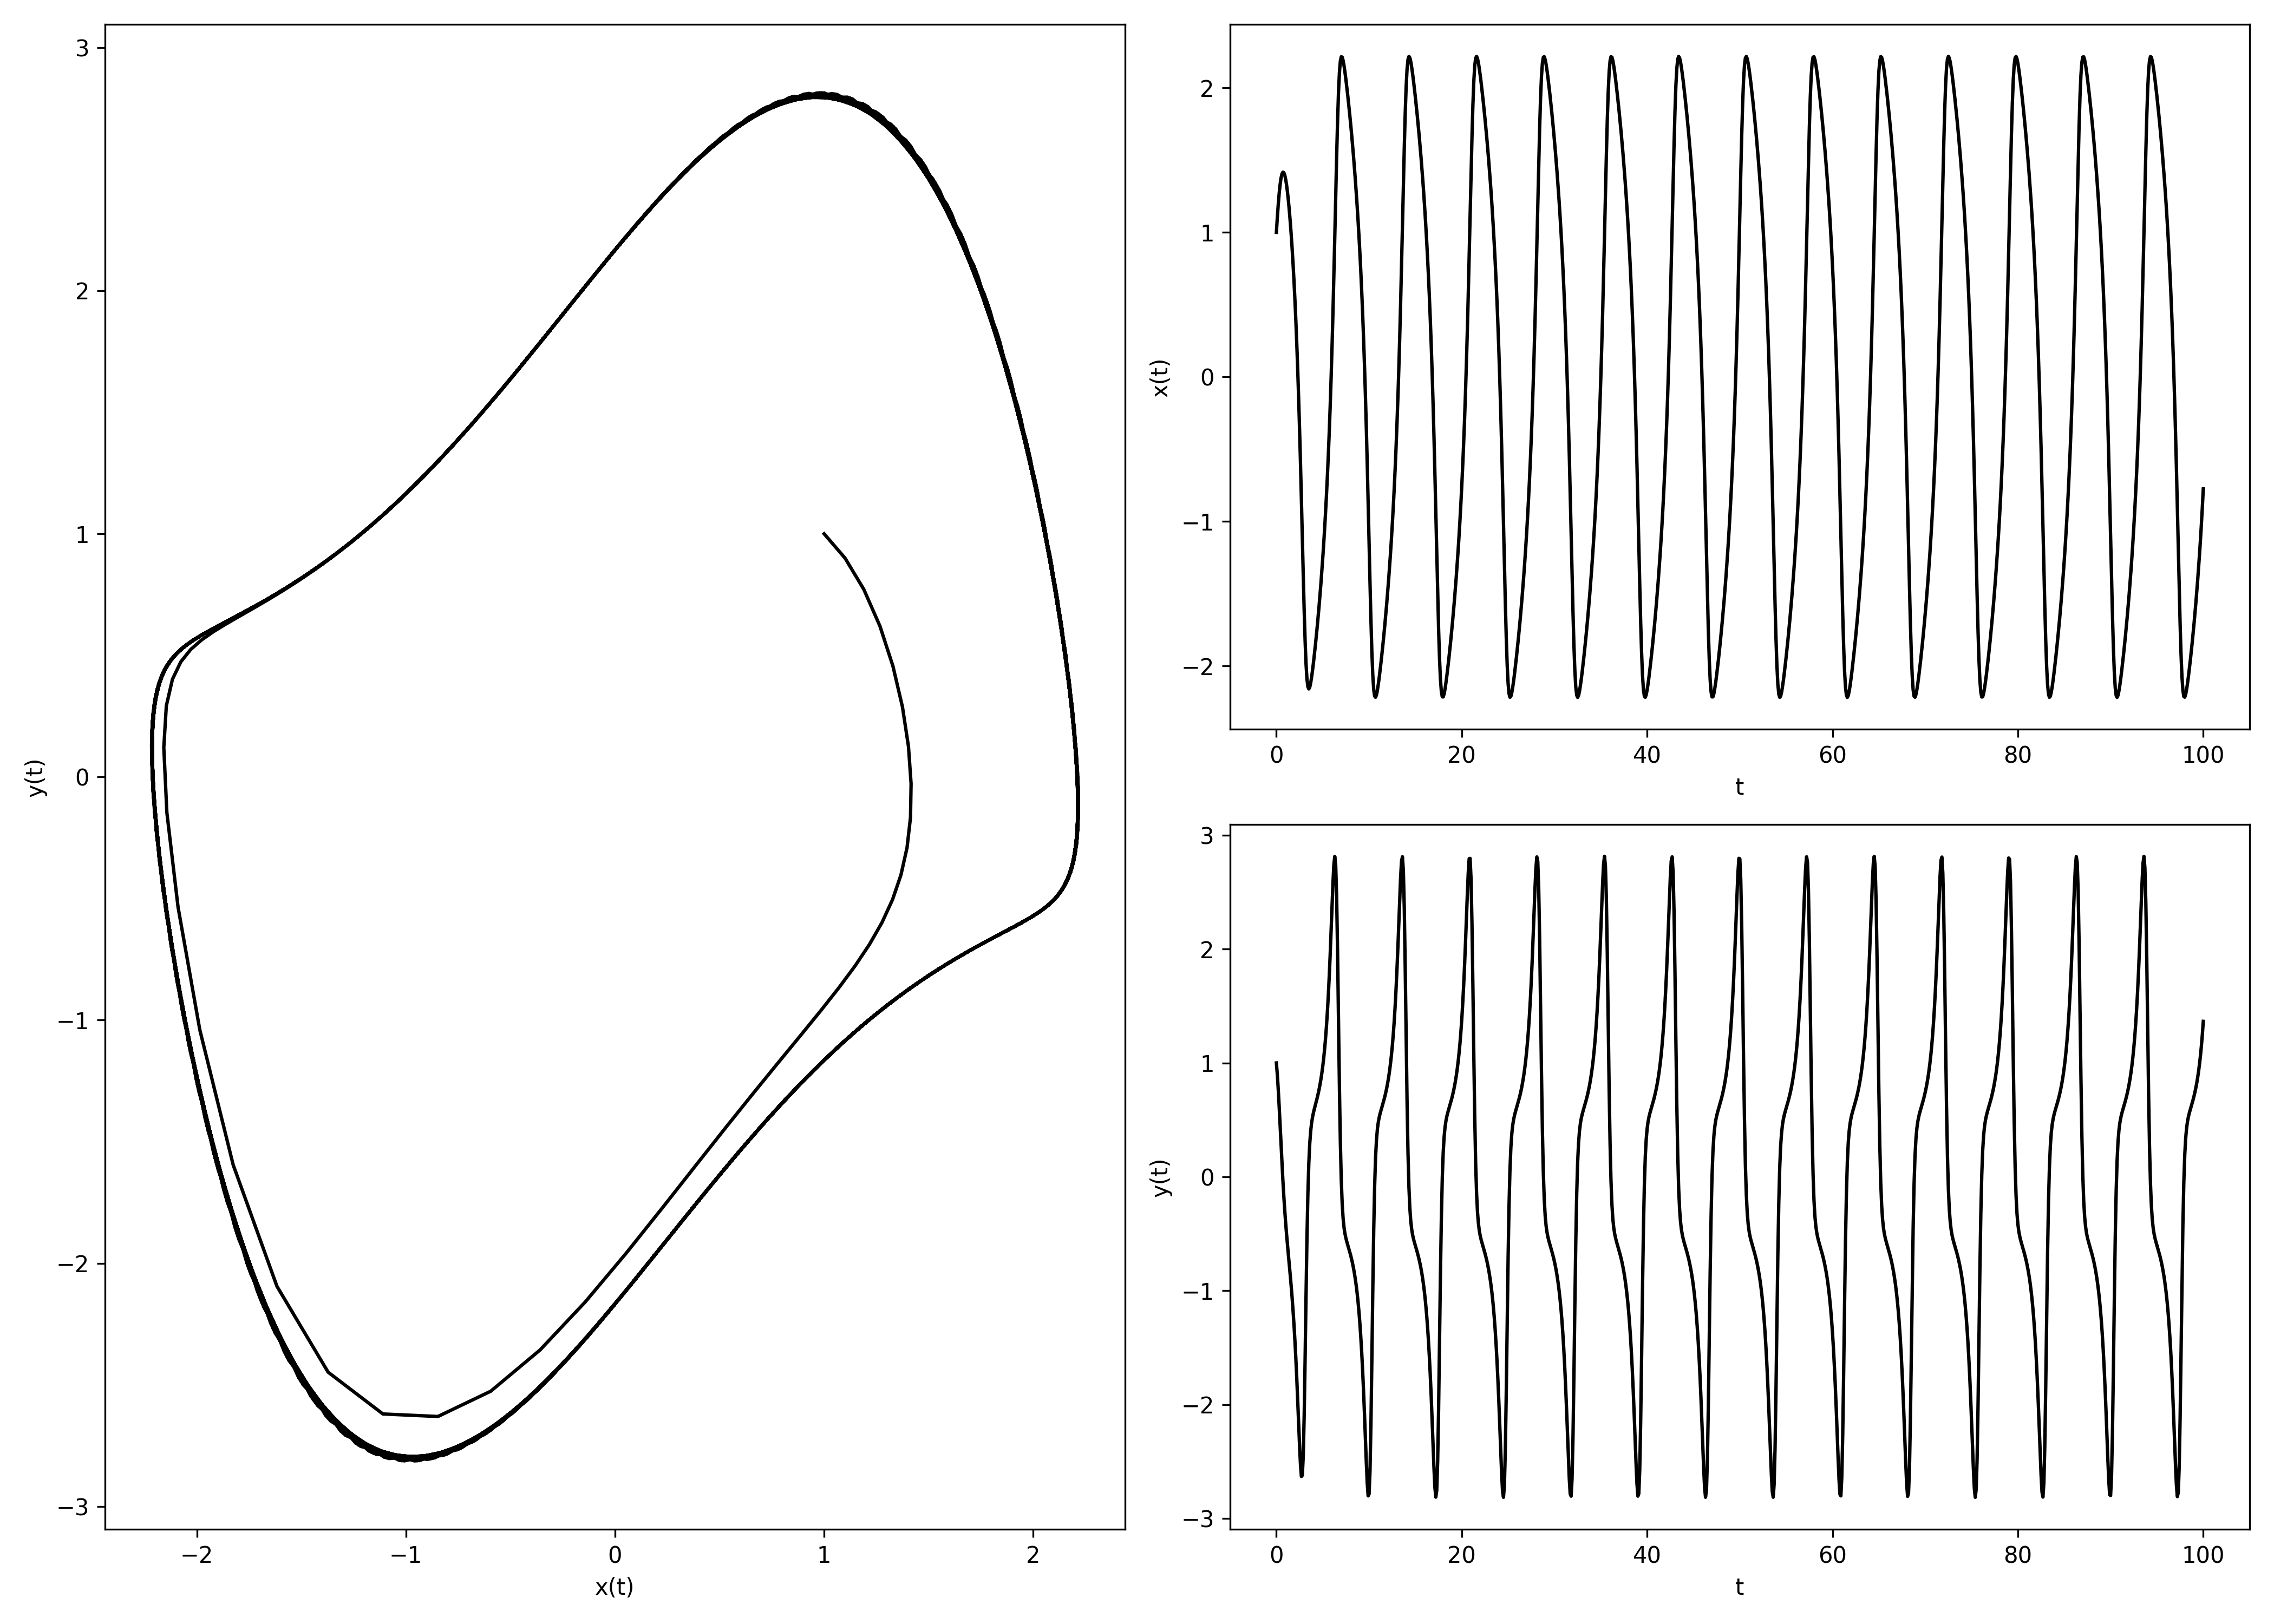
\includegraphics[scale=0.33]{x1,0y1,0mu1,0omega1,0t1,00e+02n1,00e+03.png}
\figcaption{$x_0=1,00, y_0=1.00, \mu=1.00, \omega=1.00, T = 100, N = 1000$}
%パラメーターmu
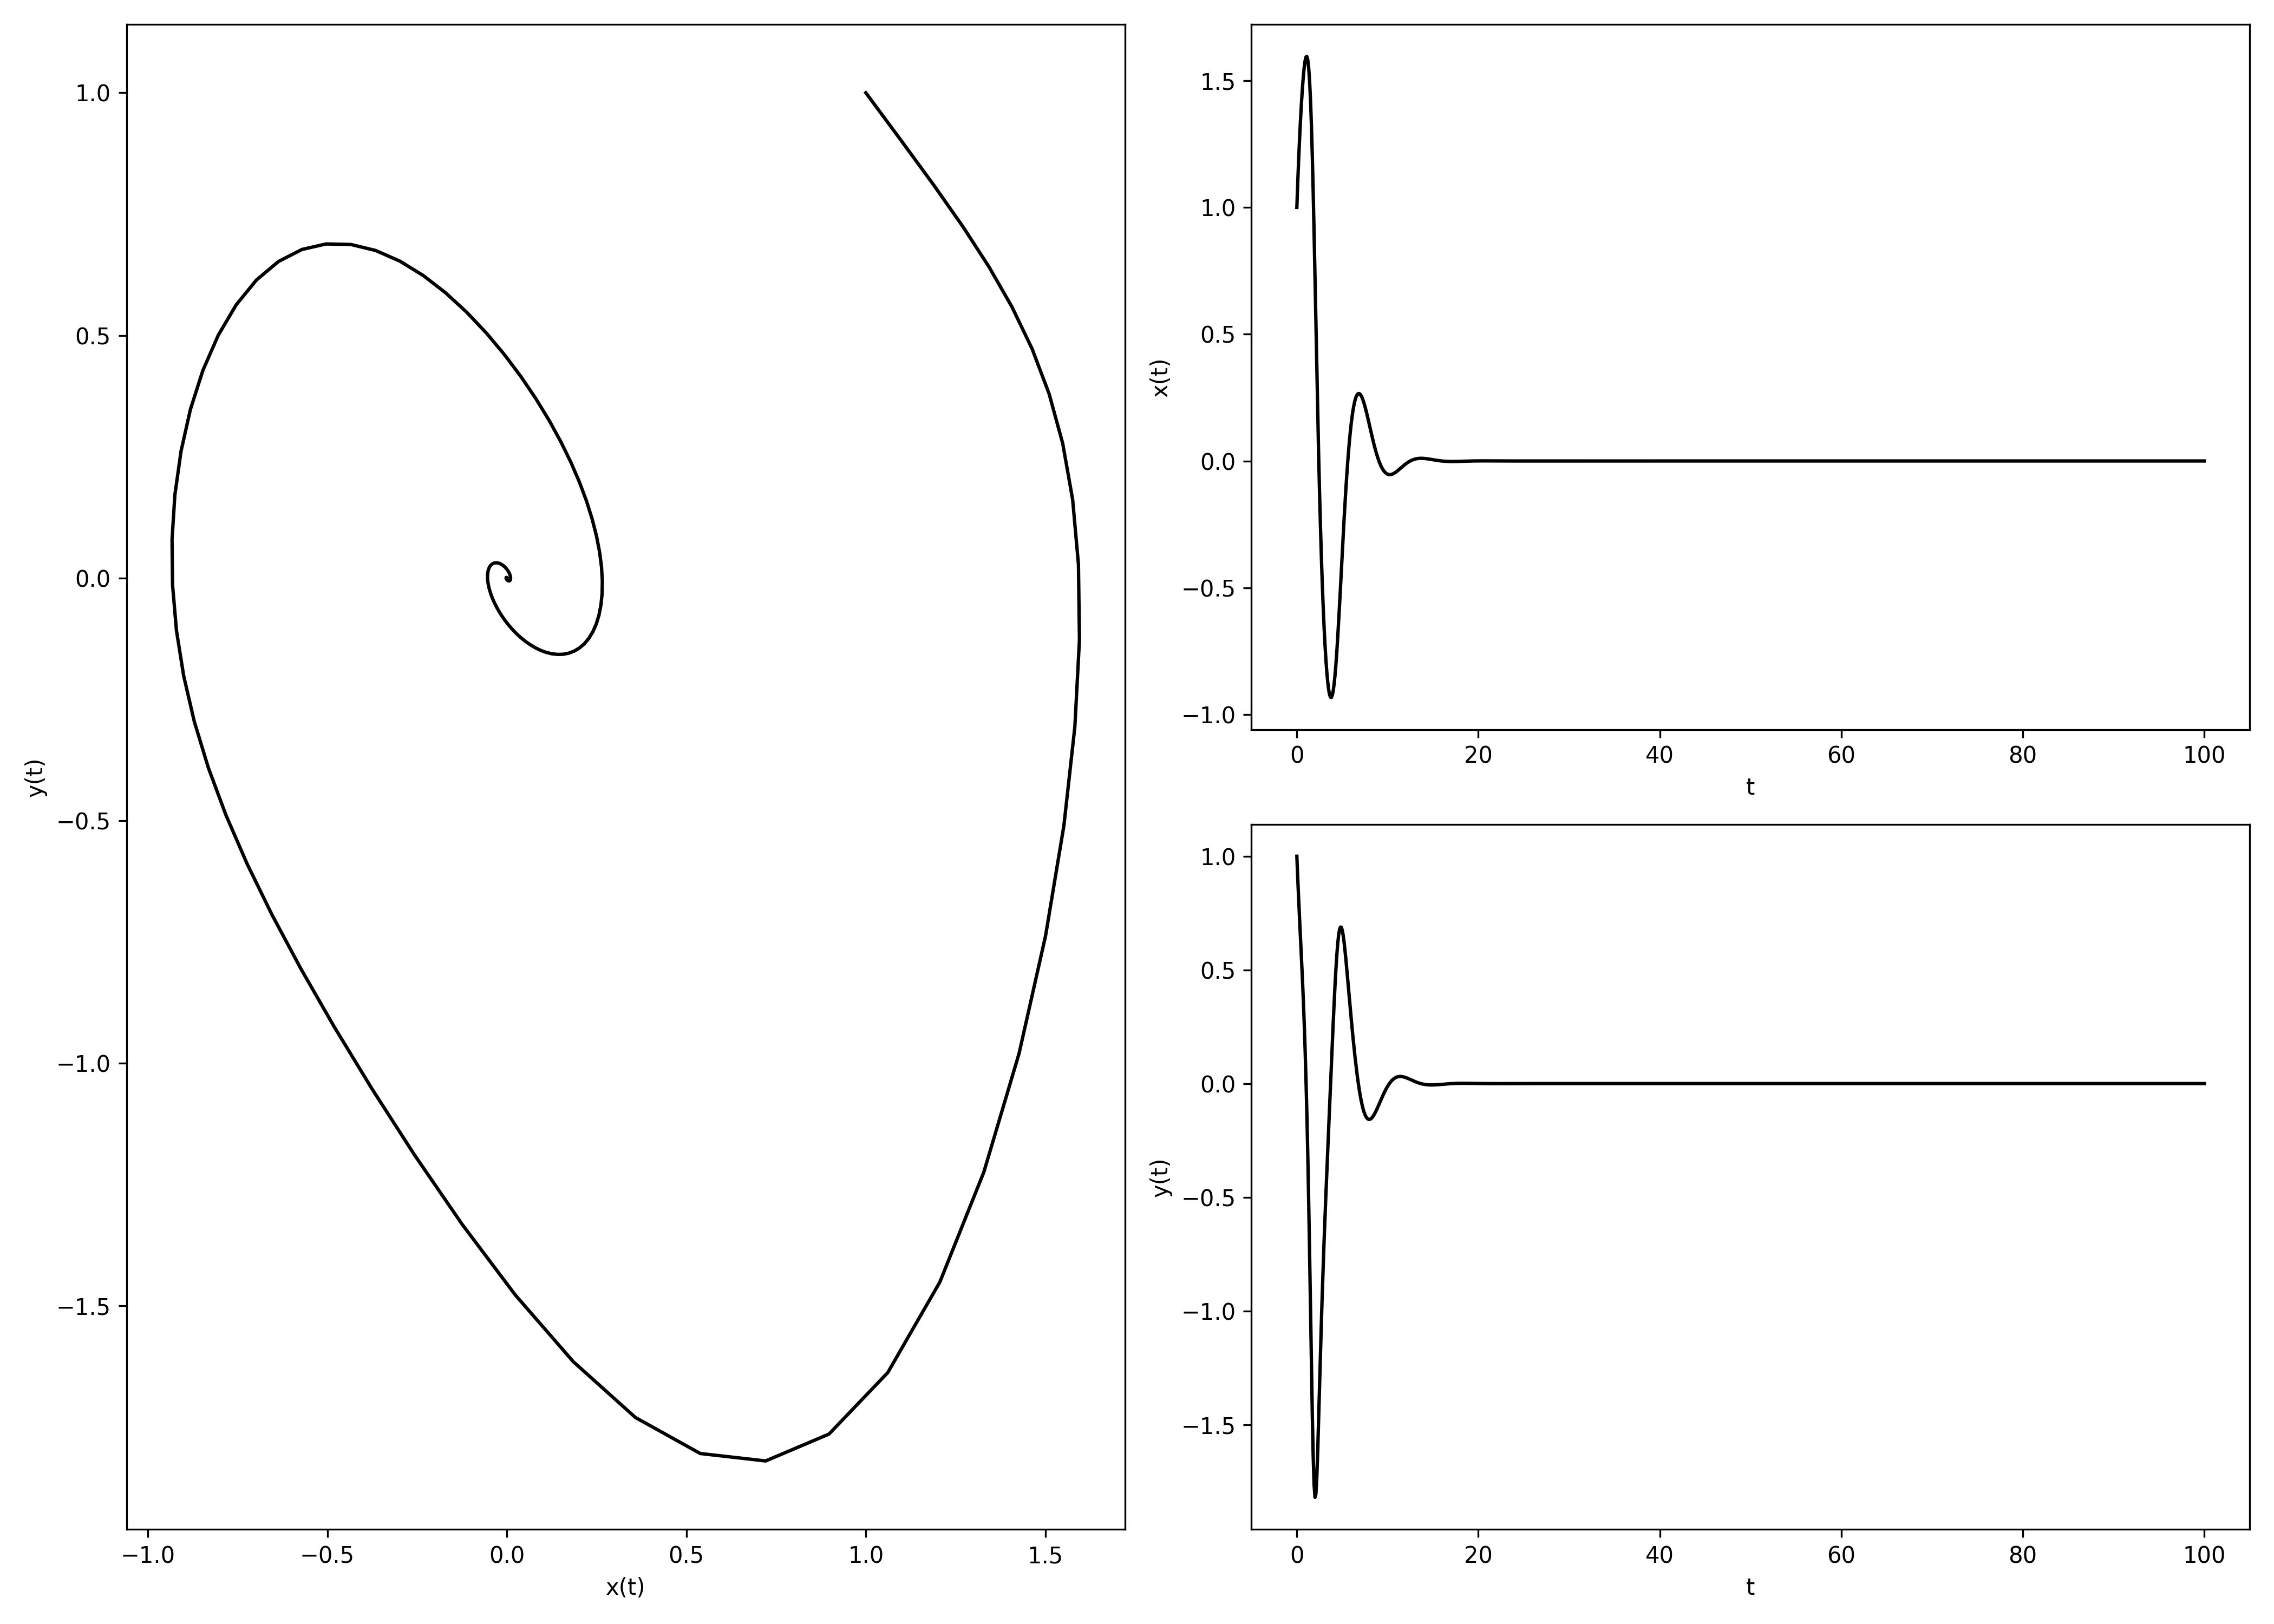
\includegraphics[scale=0.33]{x1,0y1,0mu-1,0omega1,0t1,00e+02n1,00e+03.png}
\figcaption{$x_0=1,00, y_0=1.00, \mu=-1.00, \omega=1.00, T = 100, N = 1000$}
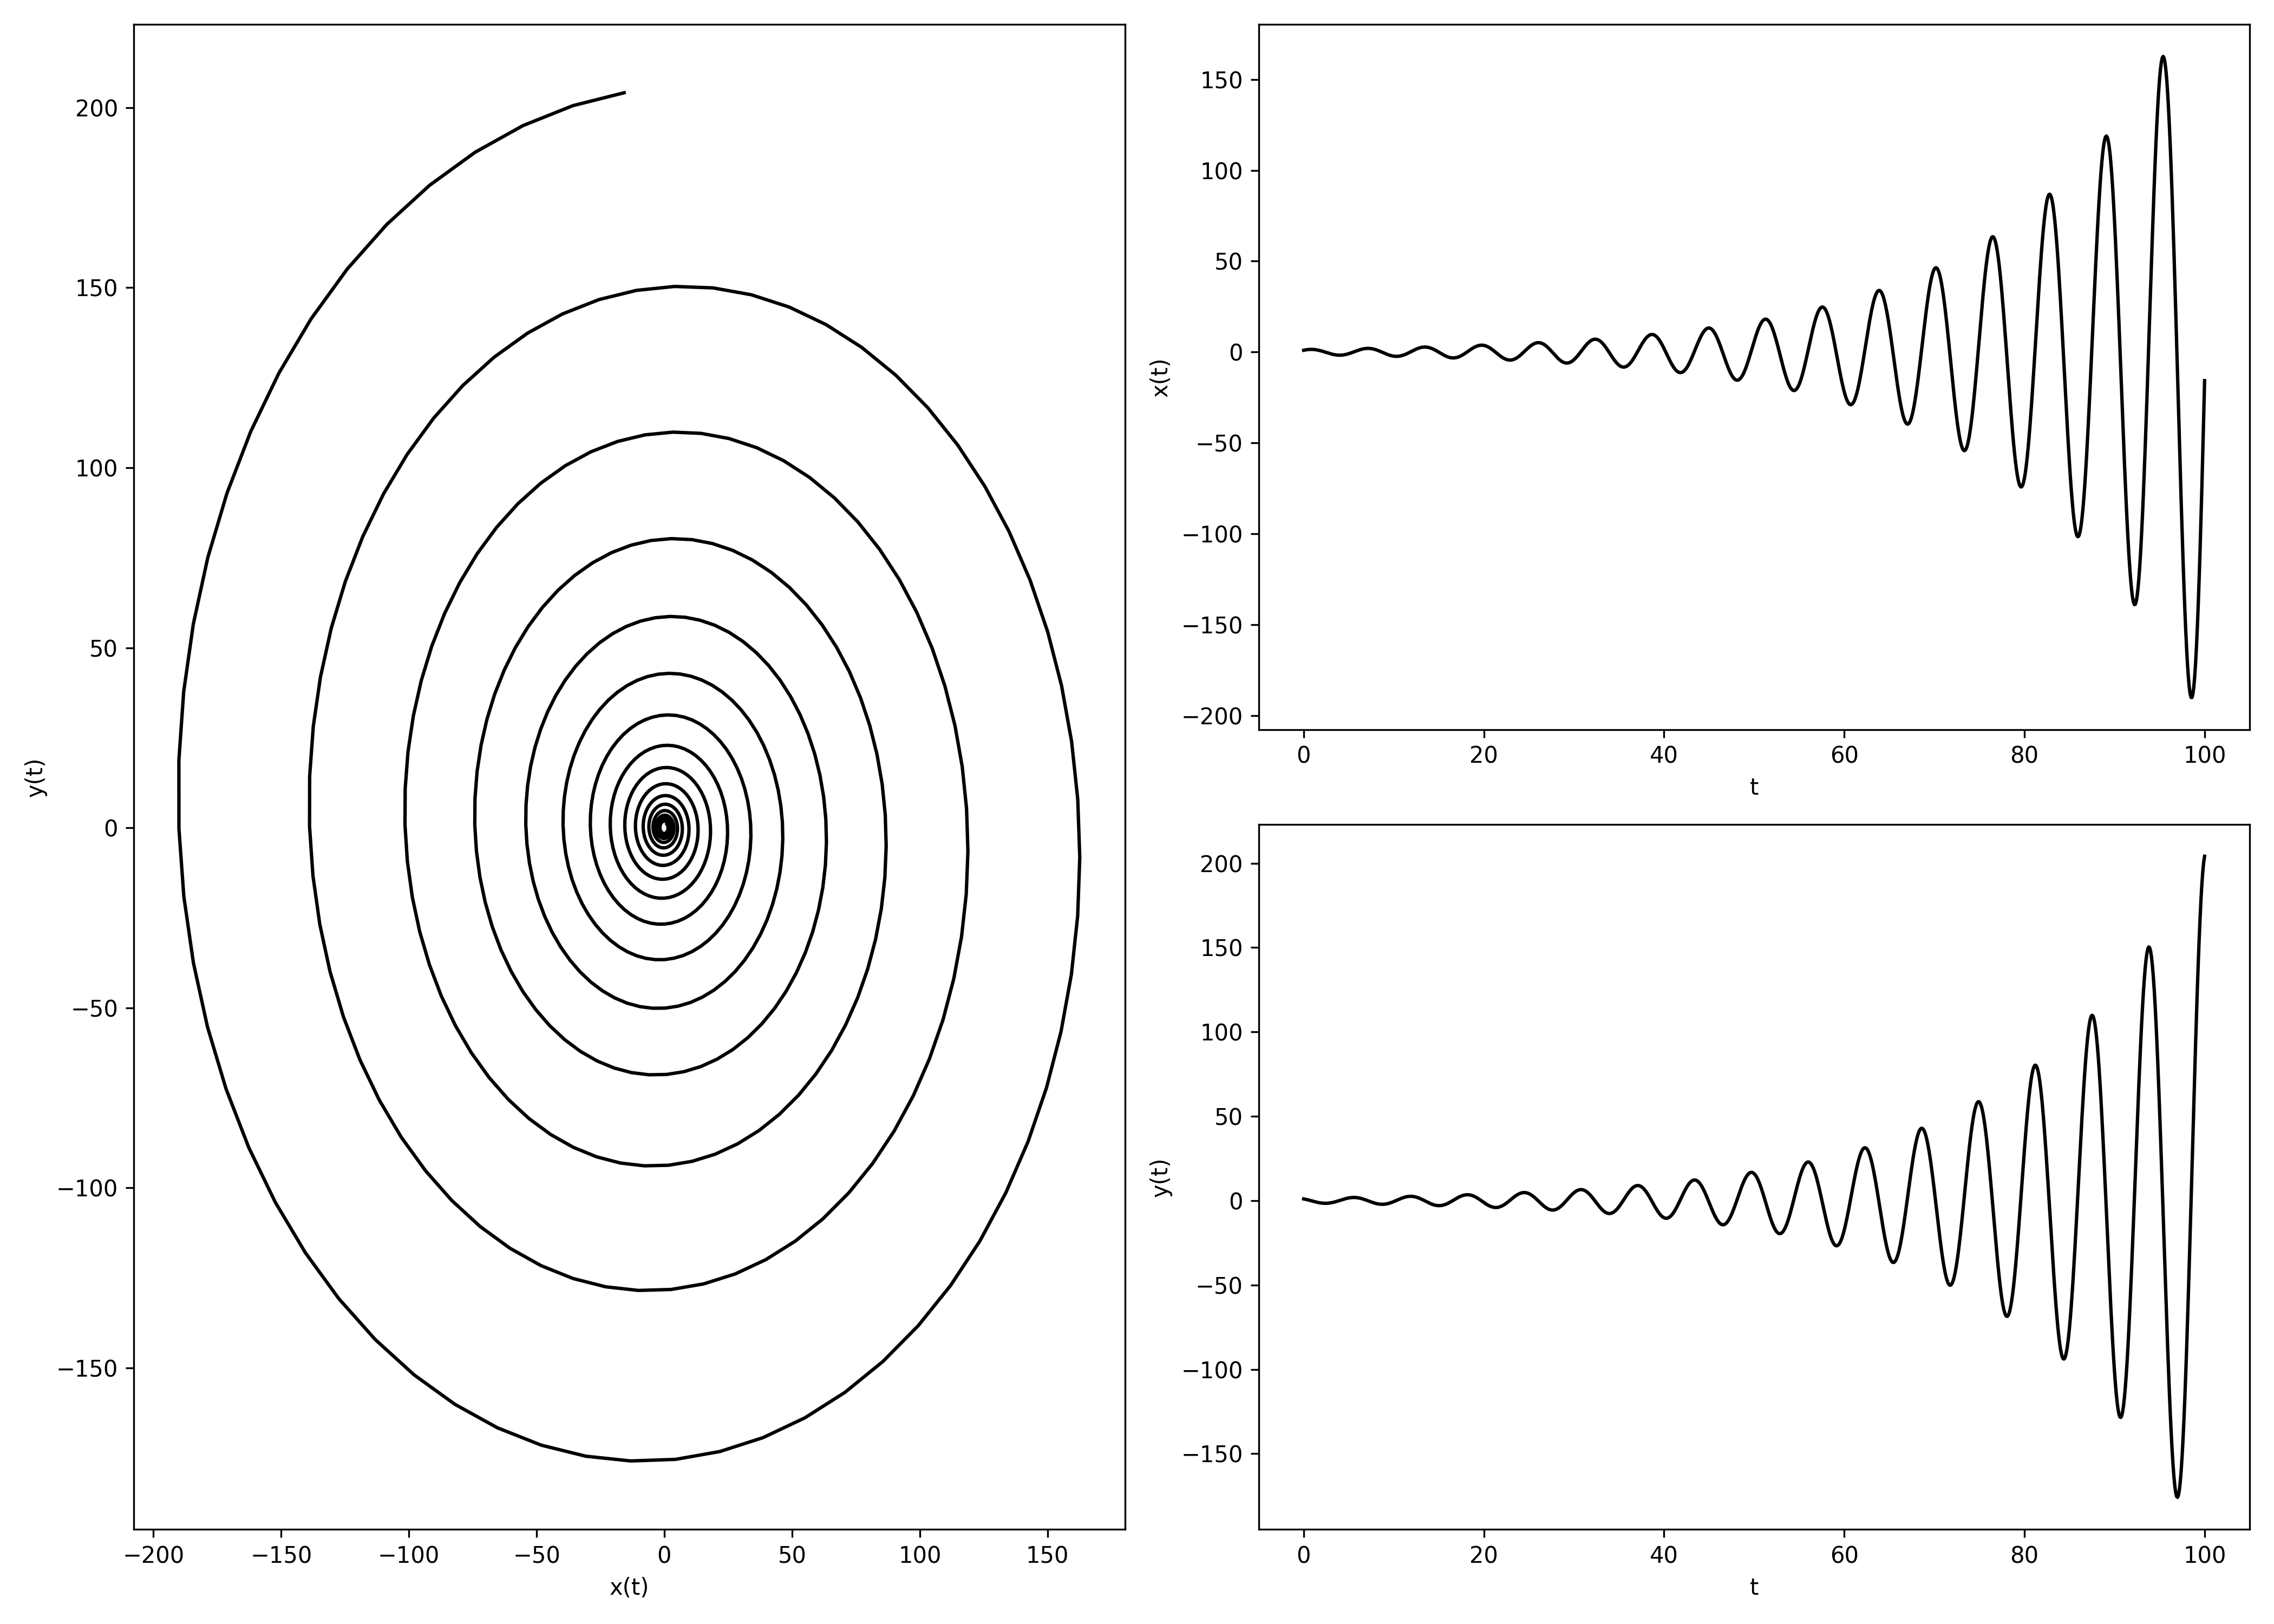
\includegraphics[scale=0.33]{x1,0y1,0mu0,0omega1,0t1,00e+02n1,00e+03.png}
\figcaption{$x_0=1,00, y_0=1.00, \mu=0.00, \omega=1.00, T = 100, N = 1000$}
% 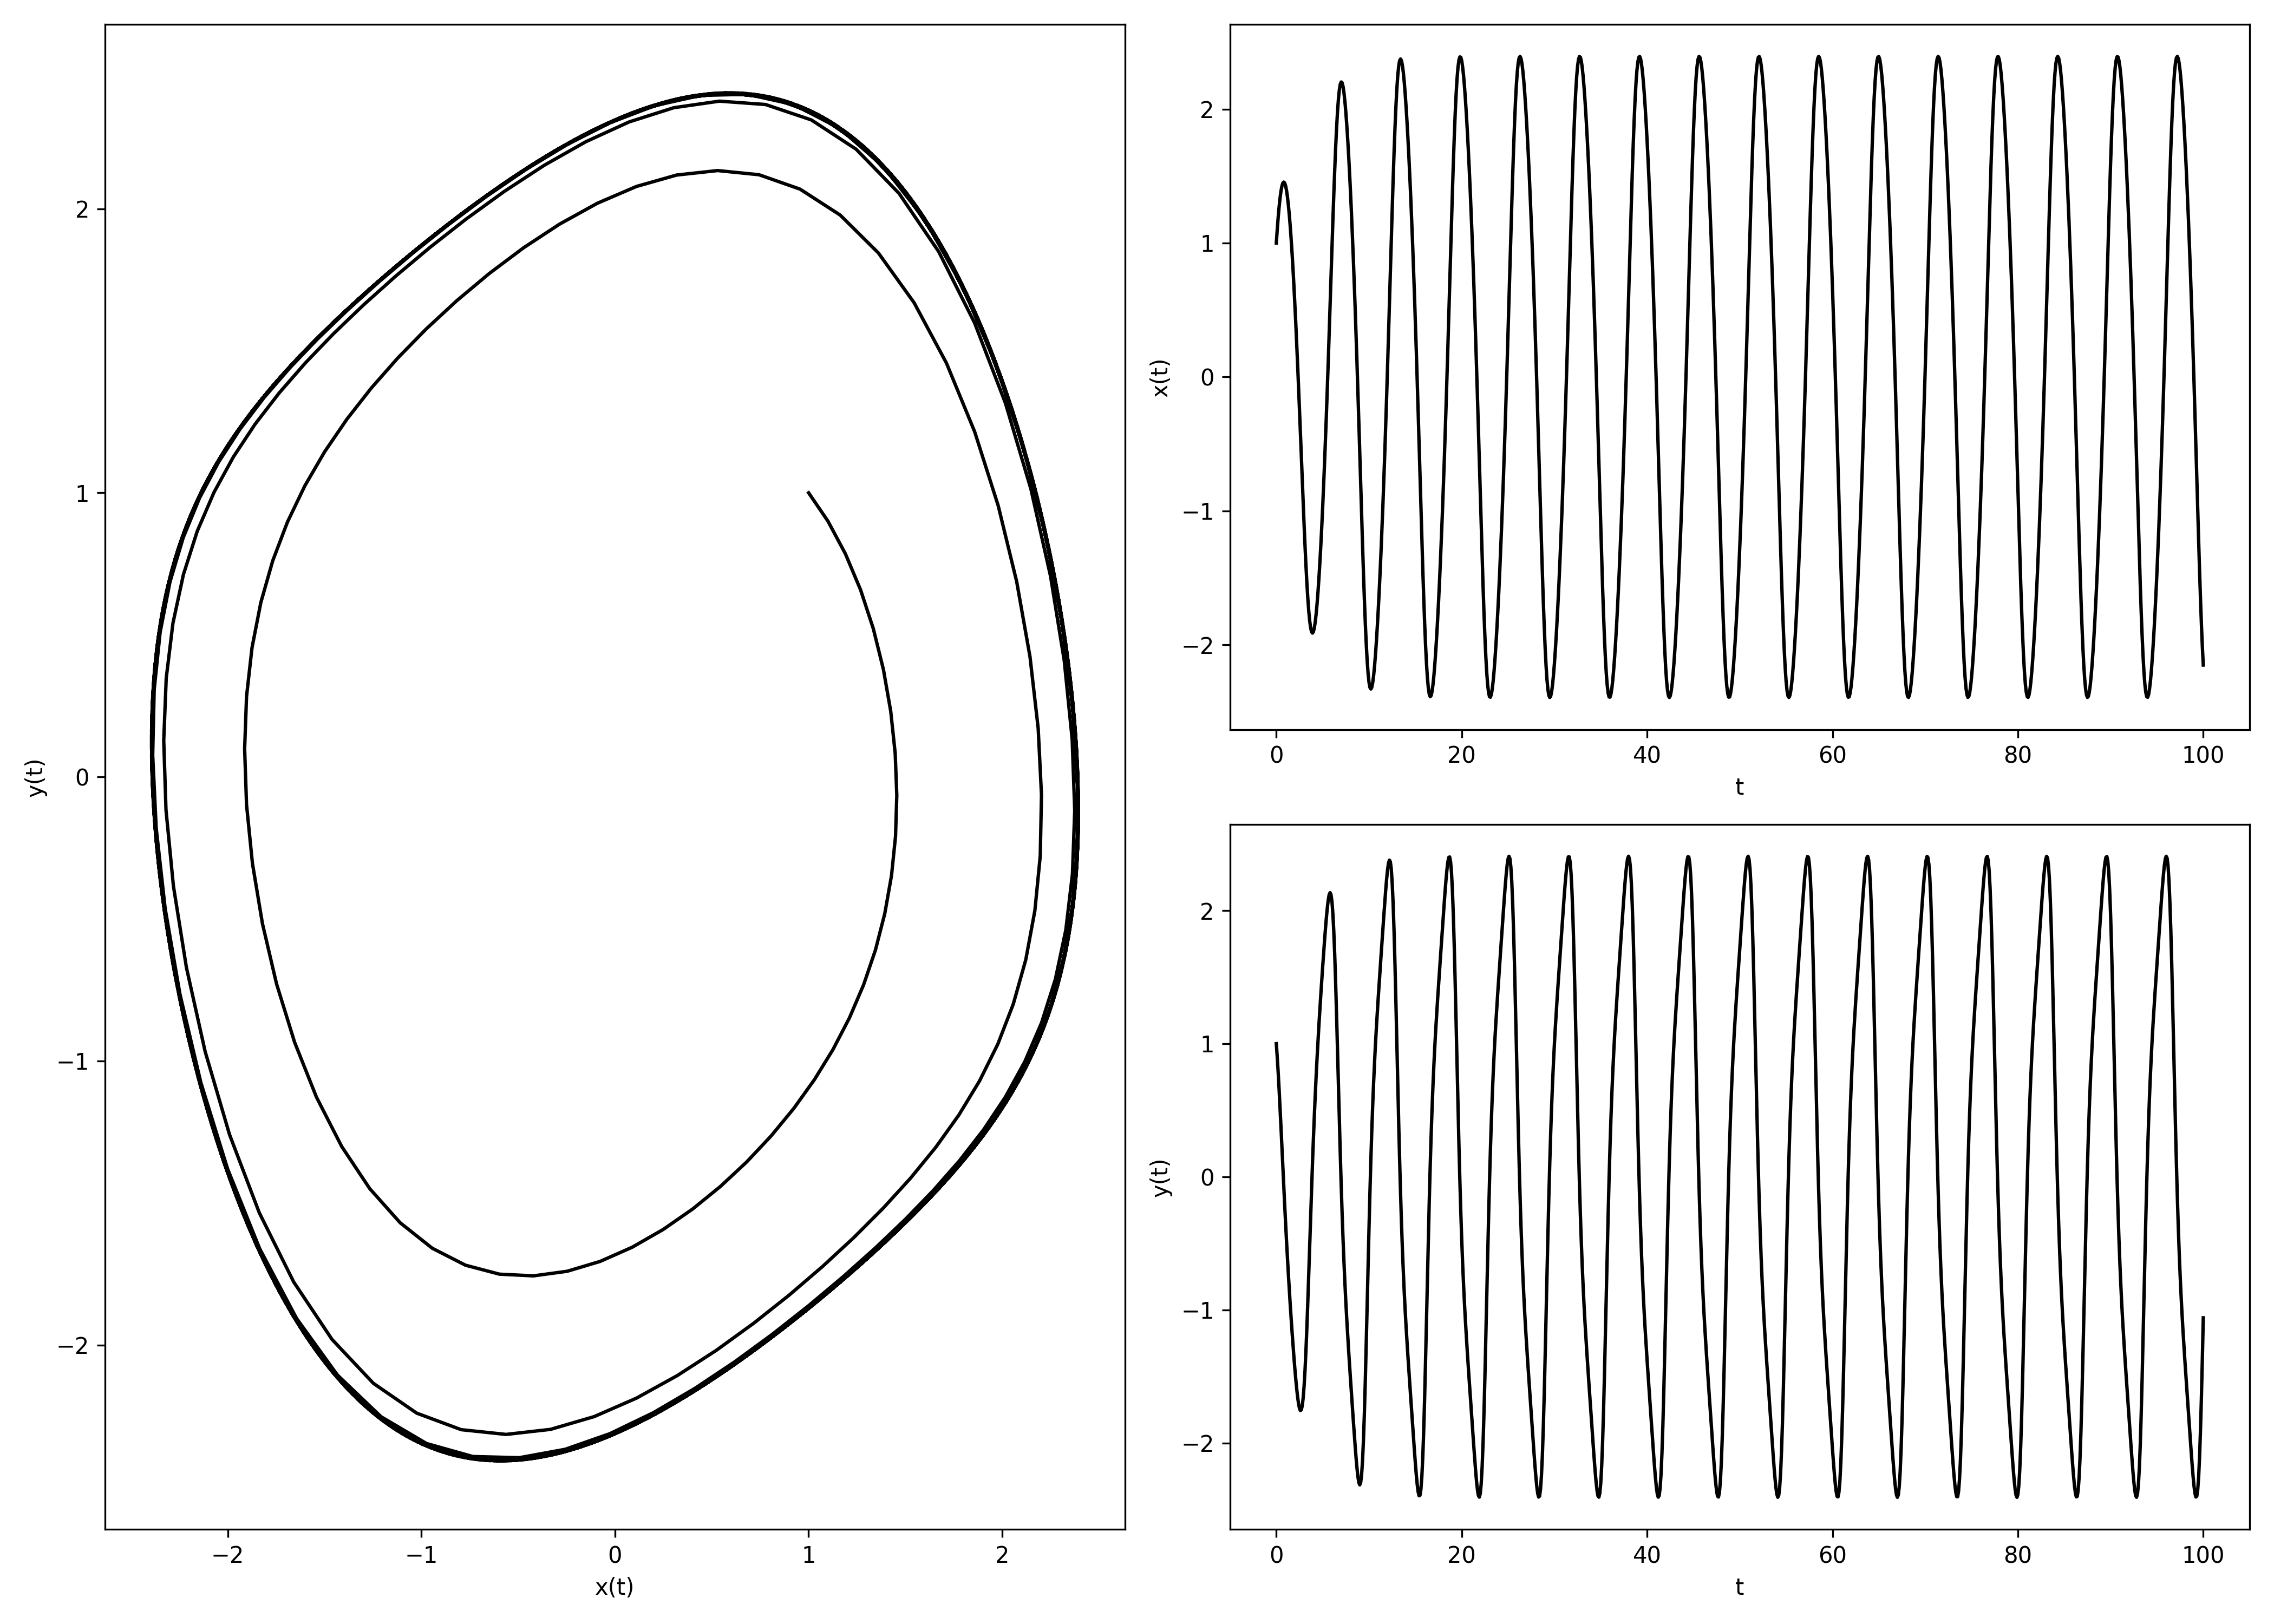
\includegraphics[scale=0.33]{x1,0y1,0mu0,2omega1,0t1,00e+02n1,00e+03.png}
% \figcaption{$x_0=1,00, y_0=1.00, \mu=0.25, \omega=1.00, T = 100, N = 1000$}
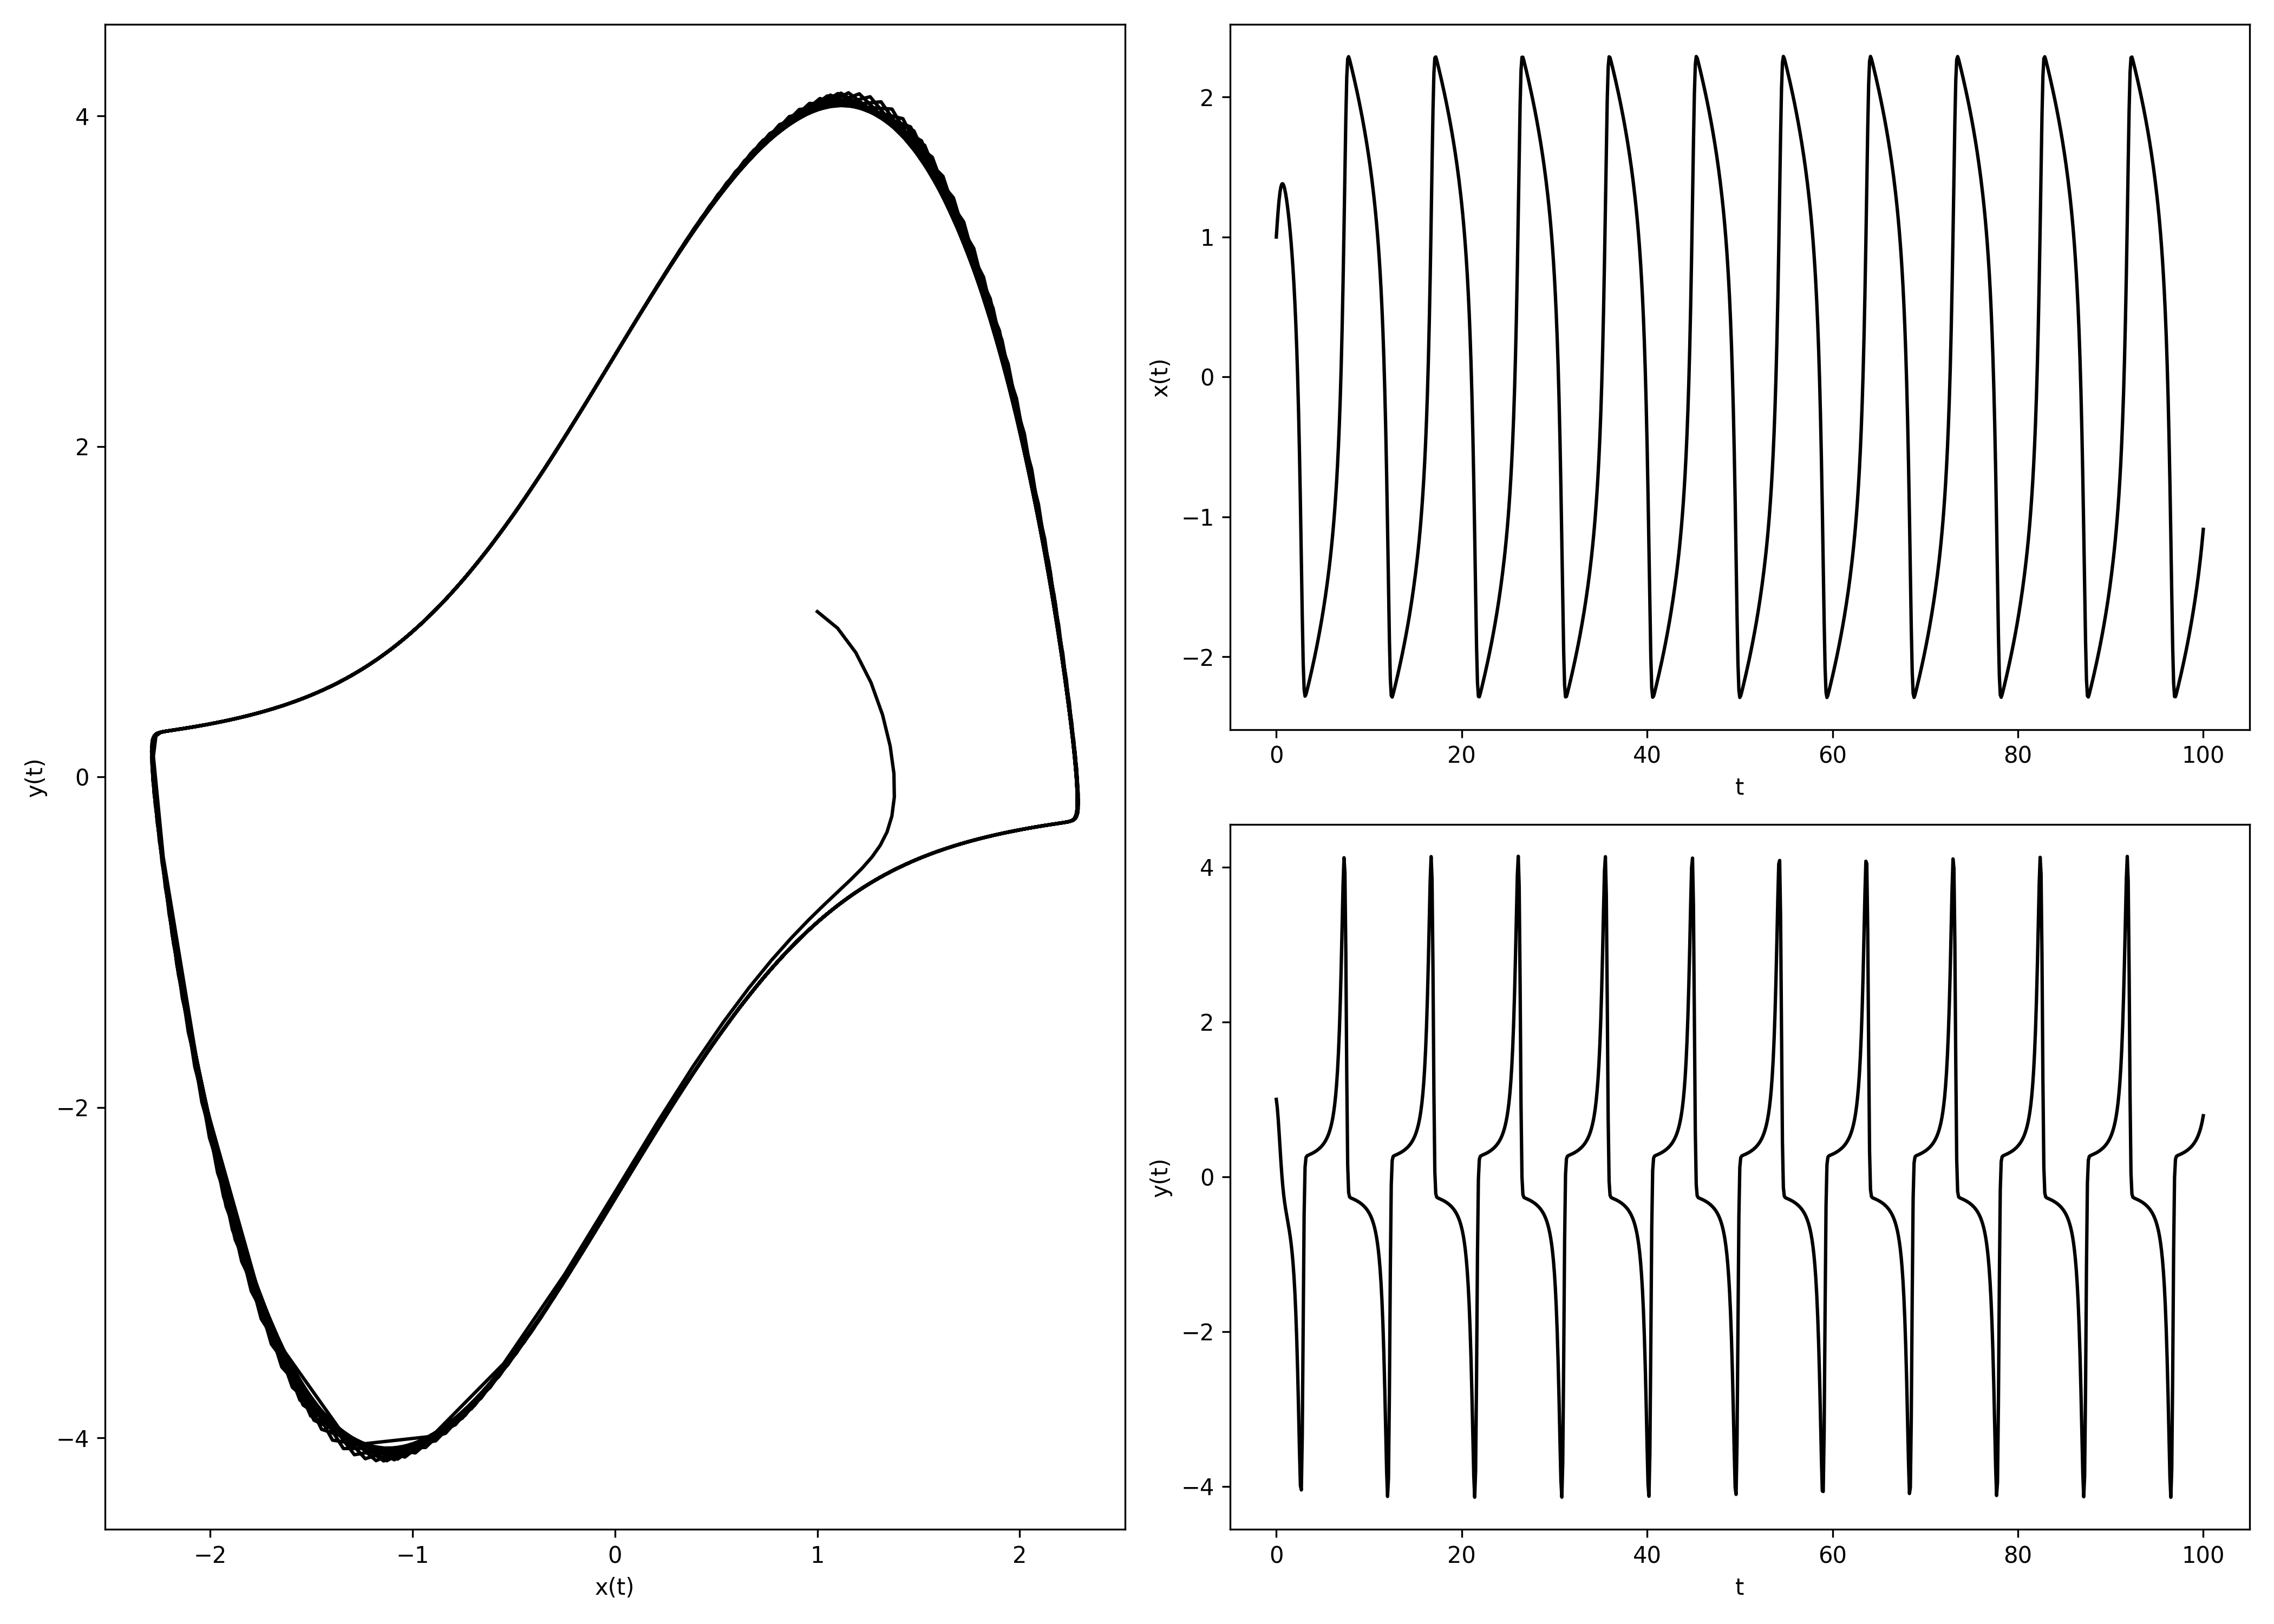
\includegraphics[scale=0.33]{x1,0y1,0mu2,0omega1,0t1,00e+02n1,00e+03.png}
\figcaption{$x_0=1,00, y_0=1.00, \mu=2.00, \omega=1.00, T = 100, N = 1000$}
%パラメーターomega
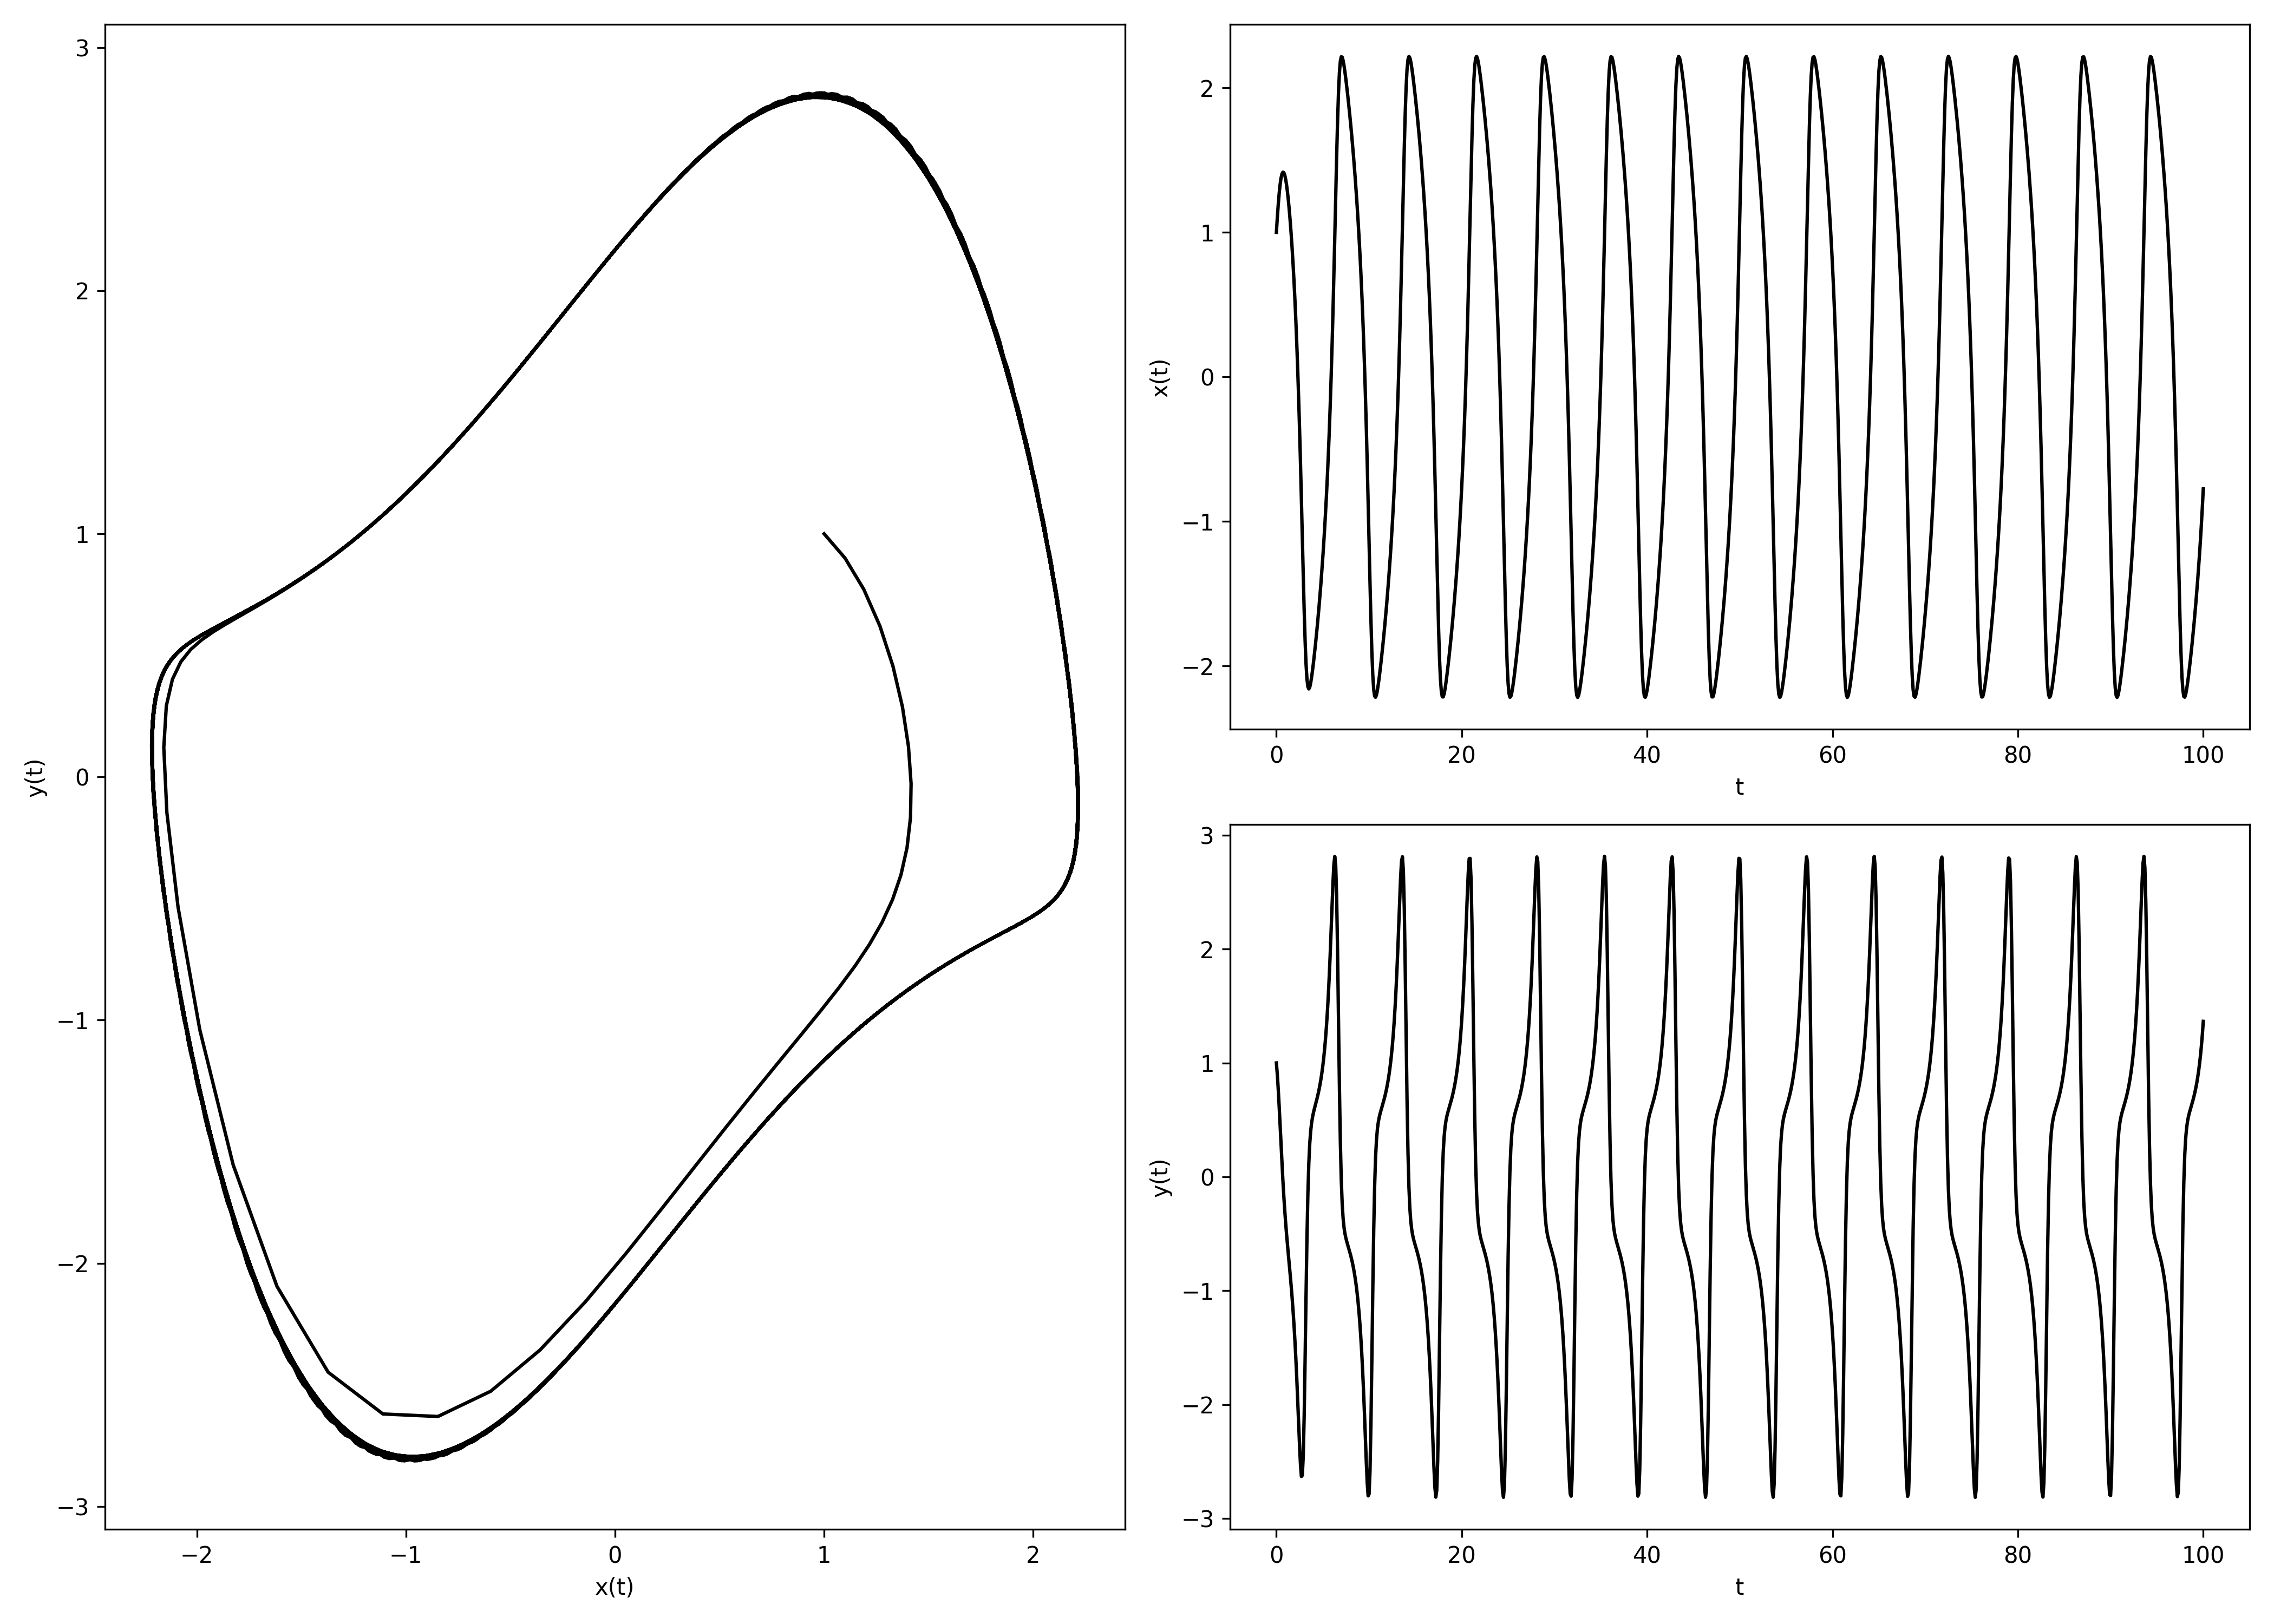
\includegraphics[scale=0.33]{x1,0y1,0mu1,0omega-1,0t1,00e+02n1,00e+03.png}
\figcaption{$x_0=1,00, y_0=1.00, \mu=1.00, \omega=-1.00, T = 100, N = 1000$}
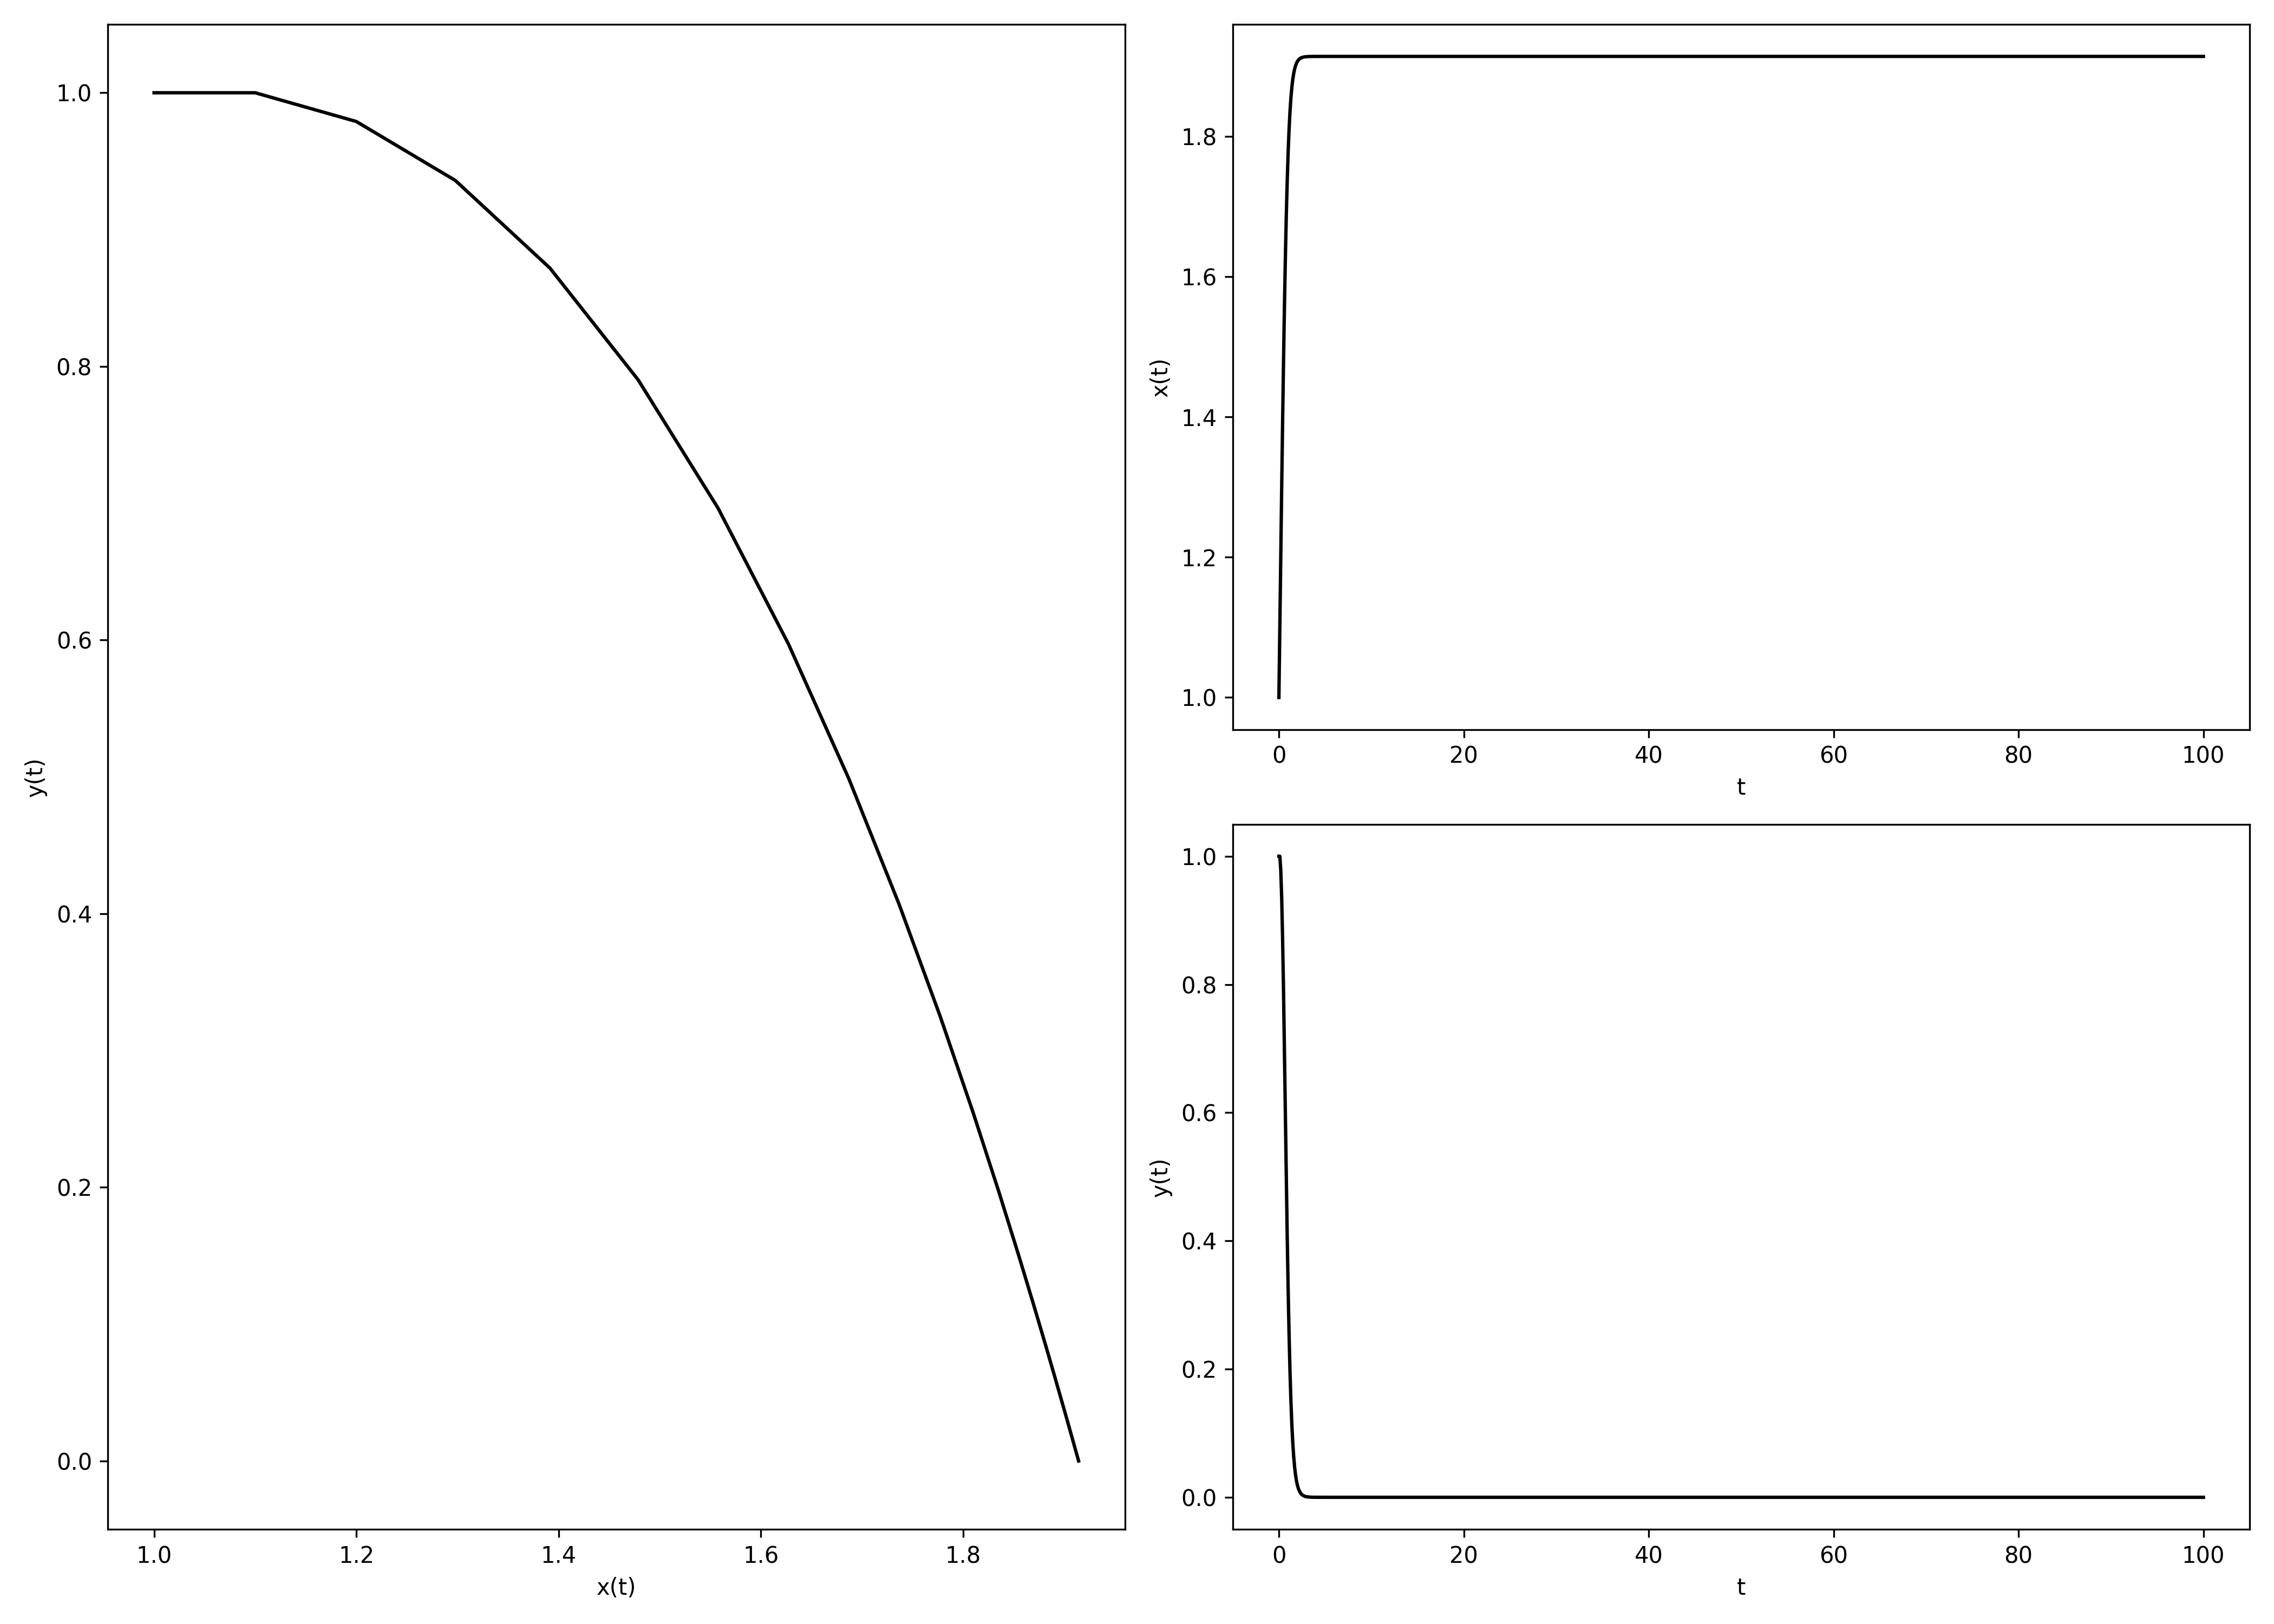
\includegraphics[scale=0.33]{x1,0y1,0mu1,0omega0,0t1,00e+02n1,00e+03.png}
\figcaption{$x_0=1,00, y_0=1.00, \mu=1.00, \omega=0.00, T = 100, N = 1000$}
% 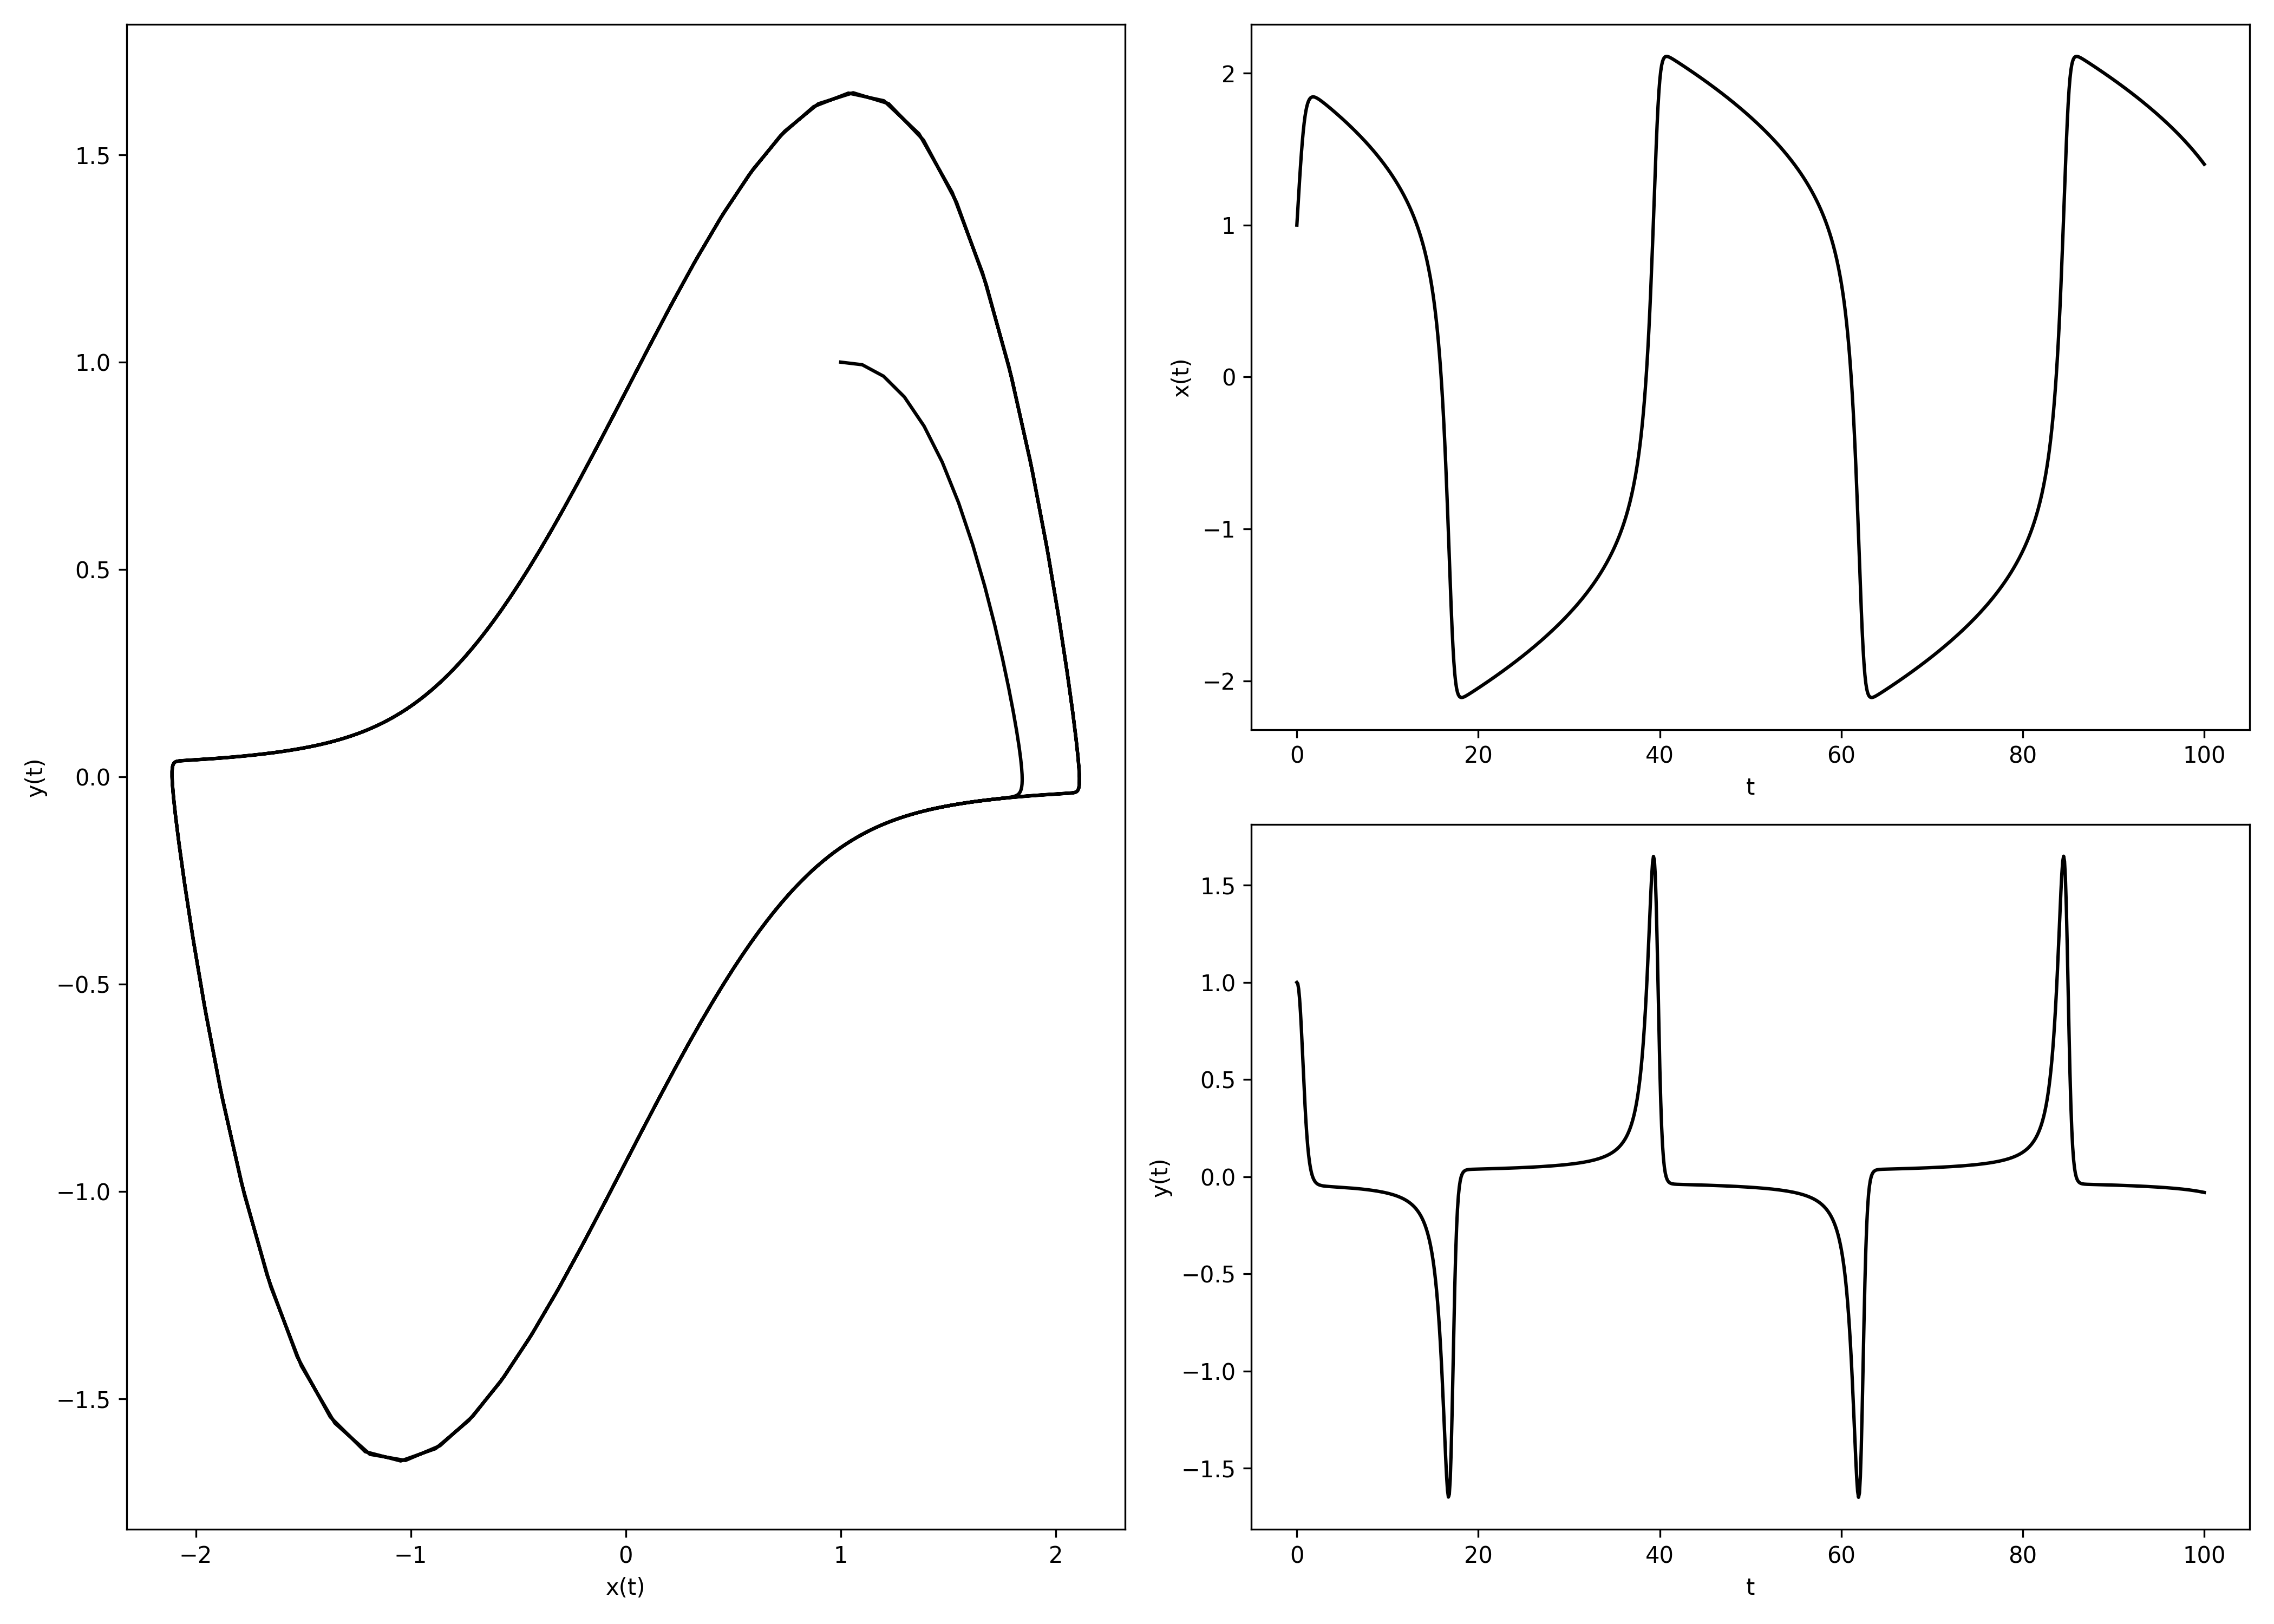
\includegraphics[scale=0.33]{x1,0y1,0mu1,0omega0,2t1,00e+02n1,00e+03.png}
% \figcaption{$x_0=1,00, y_0=1.00, \mu=1.00, \omega=0.25, T = 100, N = 1000$}
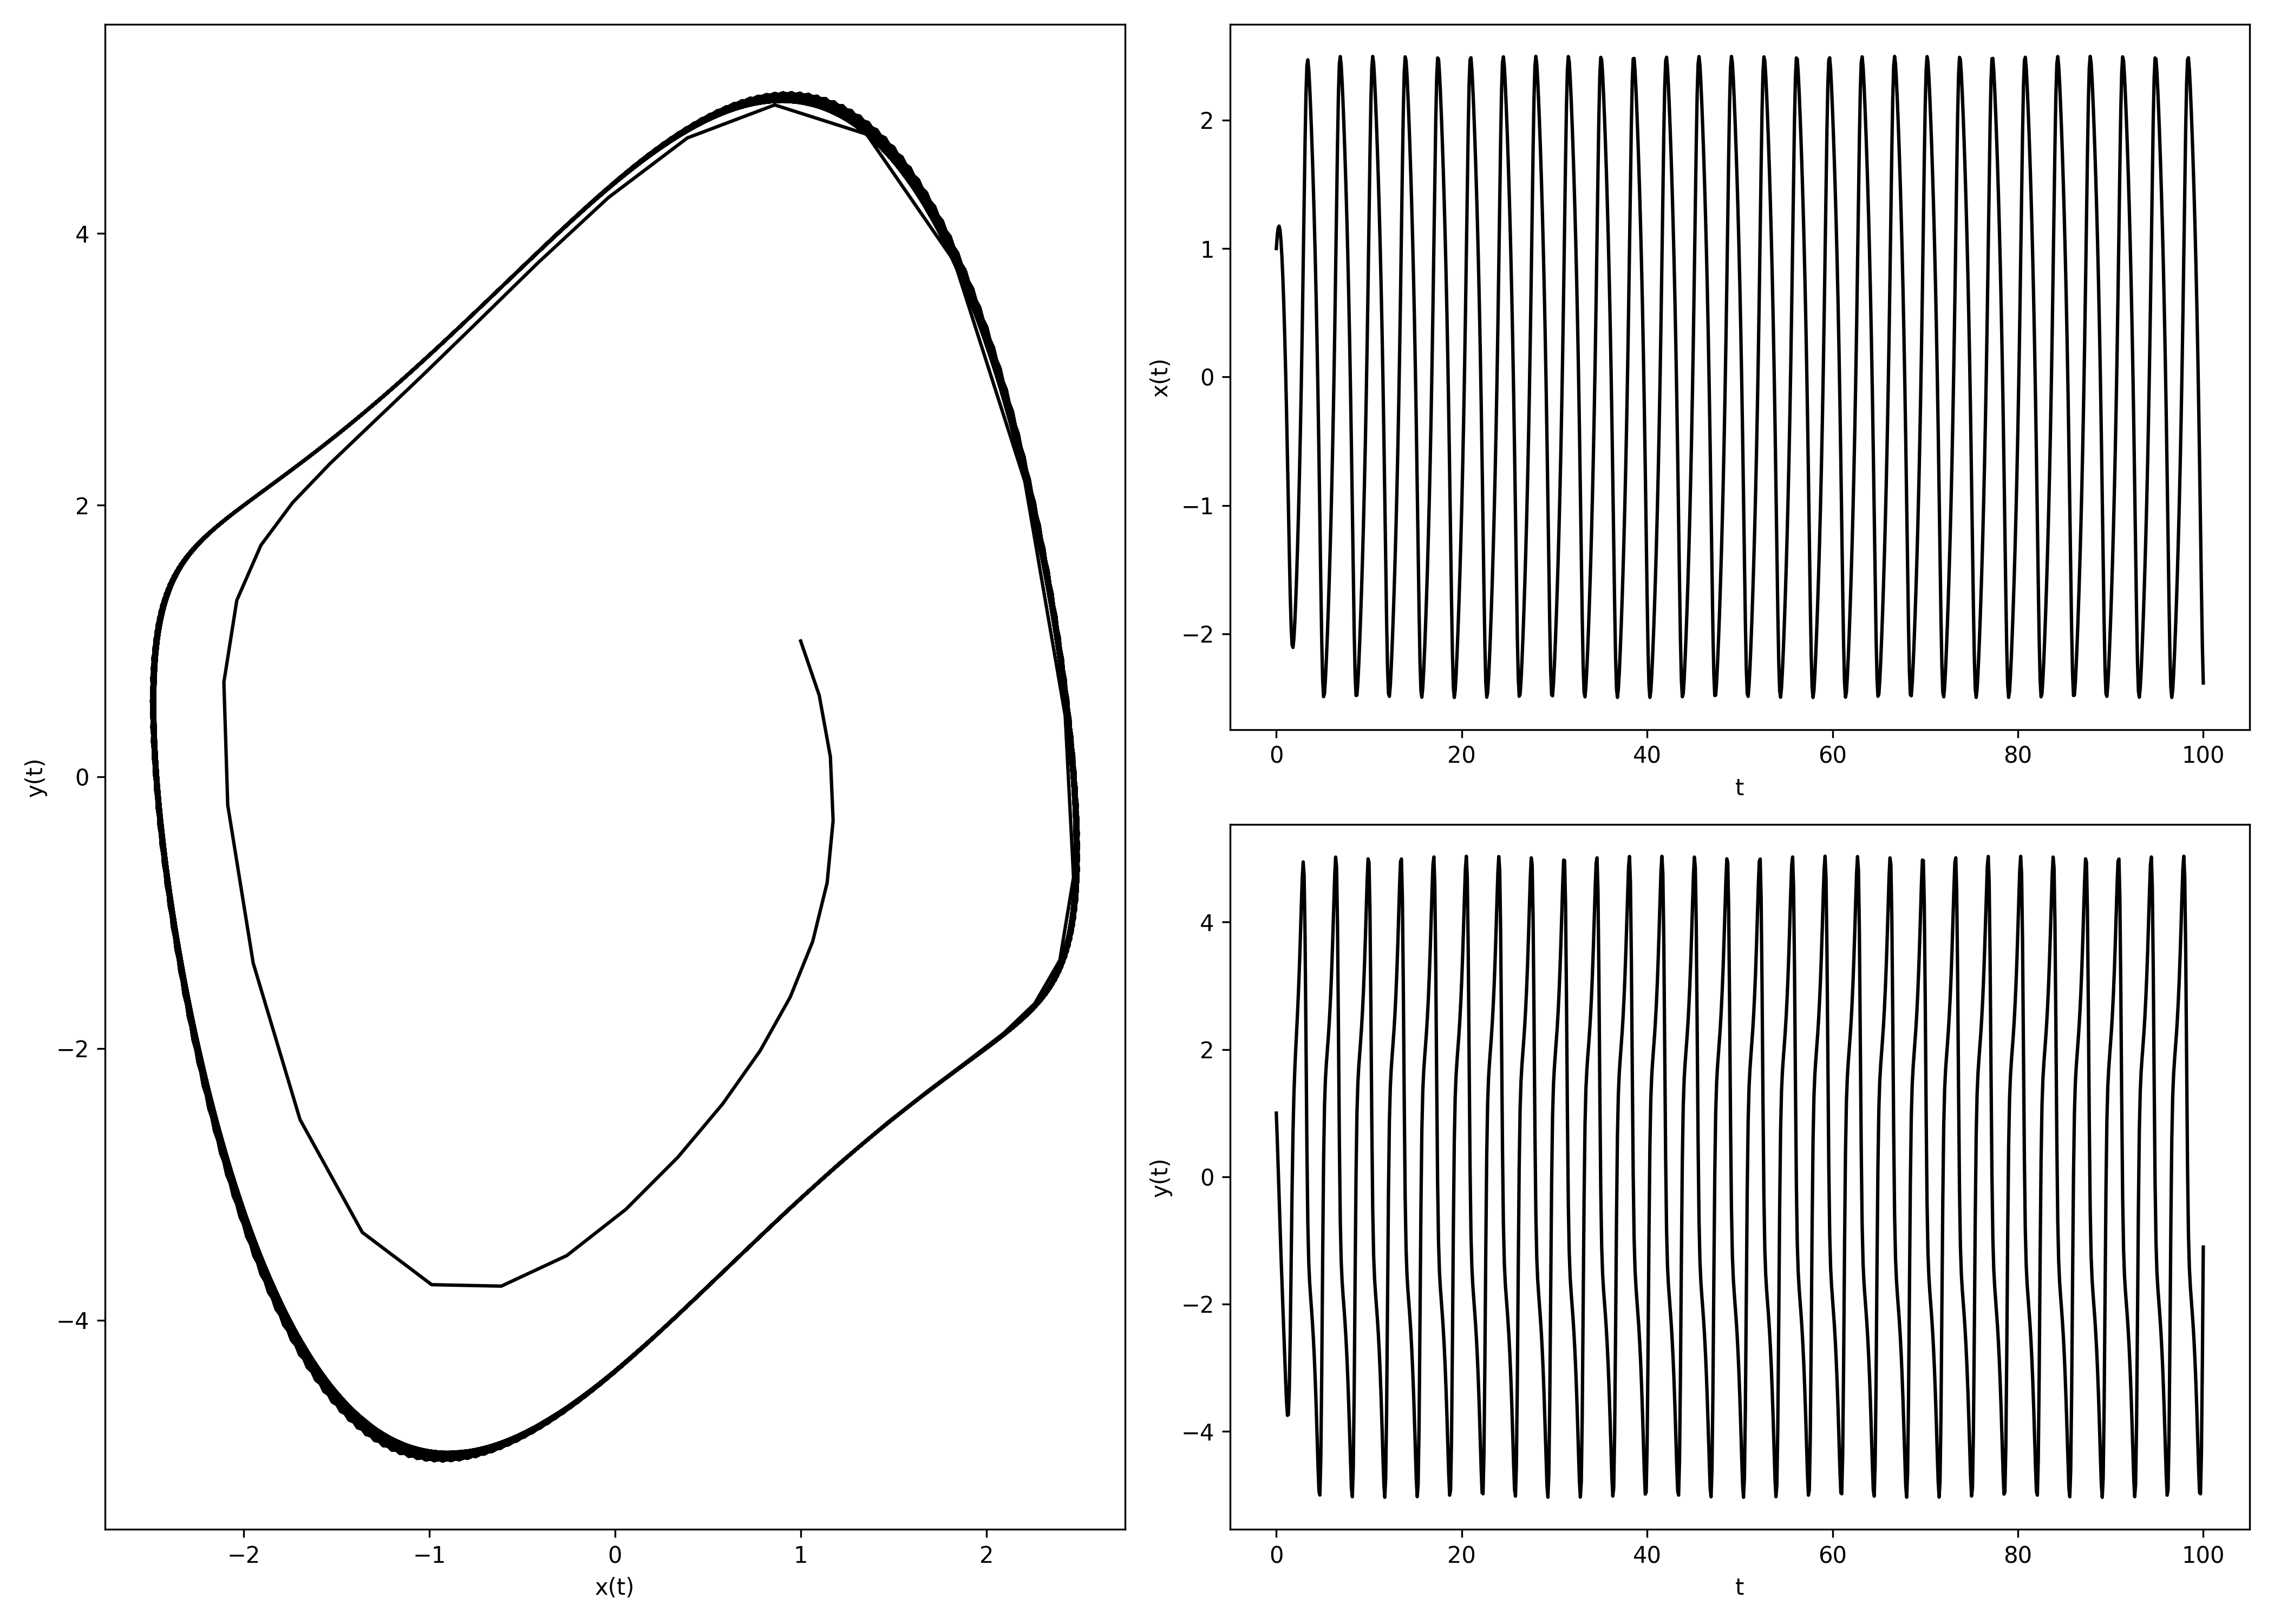
\includegraphics[scale=0.33]{x1,0y1,0mu1,0omega2,0t1,00e+02n1,00e+03.png}
\figcaption{$x_0=1,00, y_0=1.00, \mu=1.00, \omega=2.00, T = 100, N = 1000$}
%パラメーター初期値
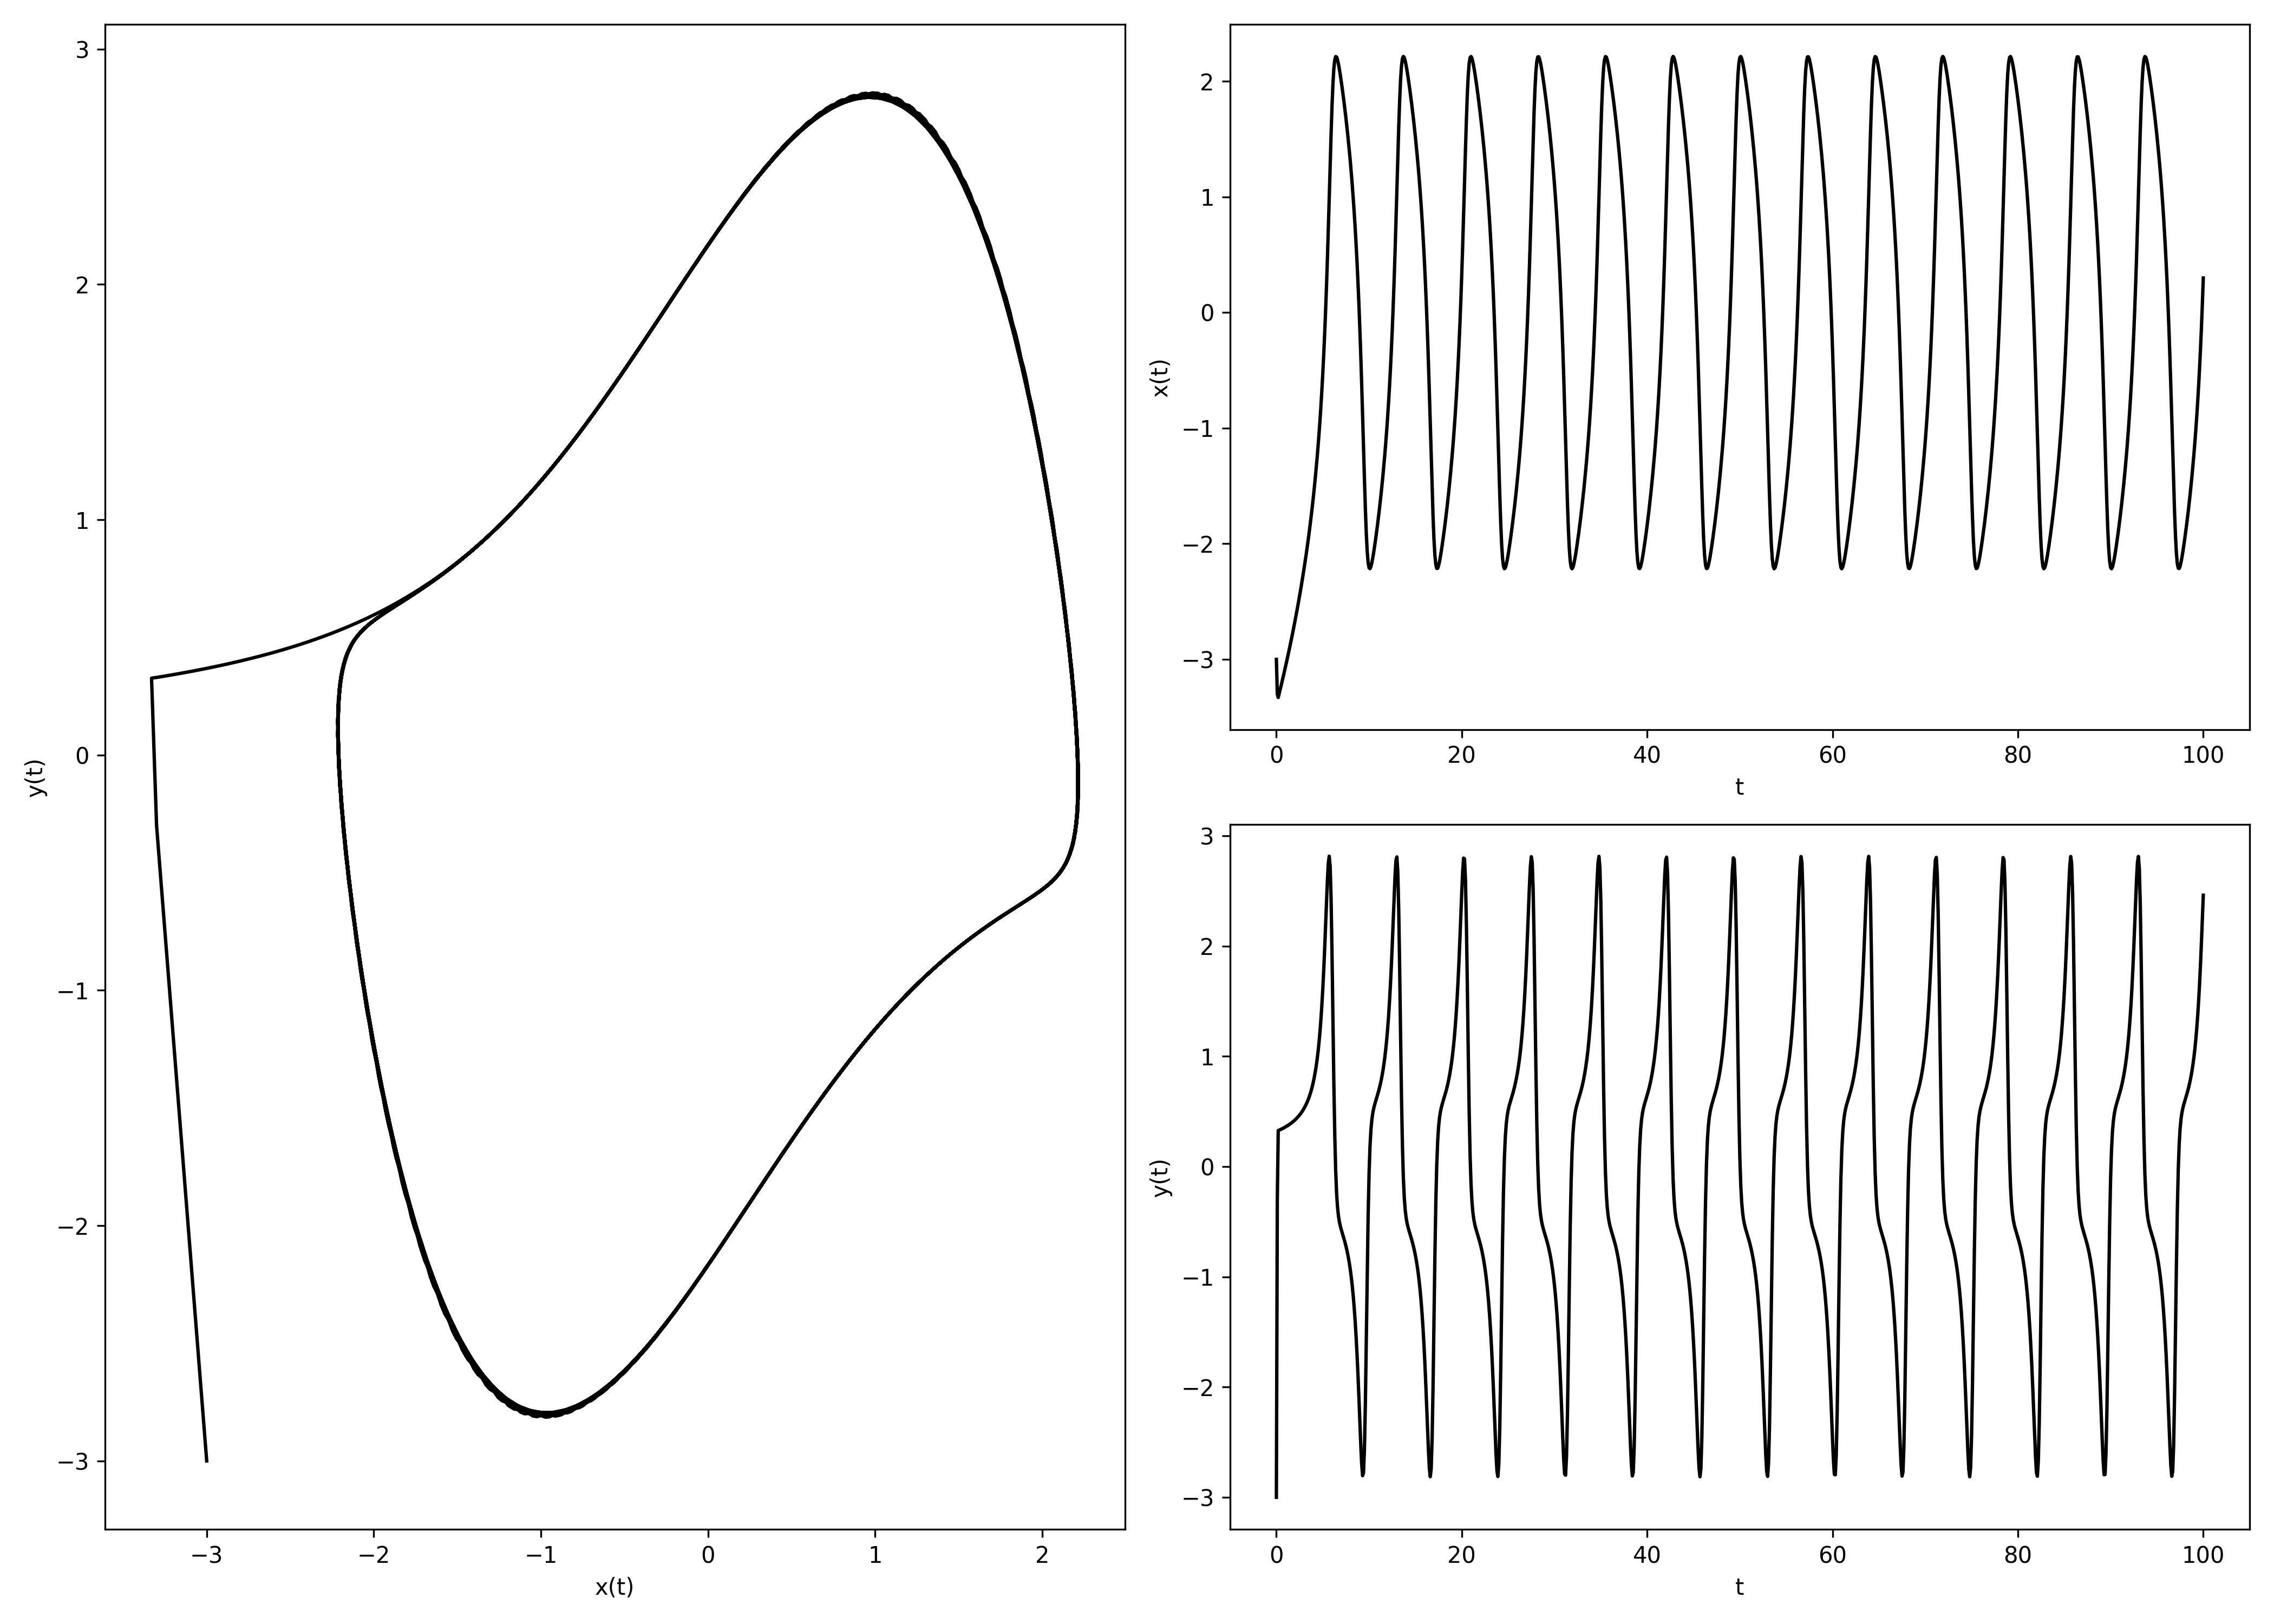
\includegraphics[scale=0.33]{x-3,0y-3,0mu1,0omega1,0t1,00e+02n1,00e+03.png}
\figcaption{$x_0=-3.00, y_0=-3.00, \mu=1,00, \omega=1.00, T = 100, N = 1000$}
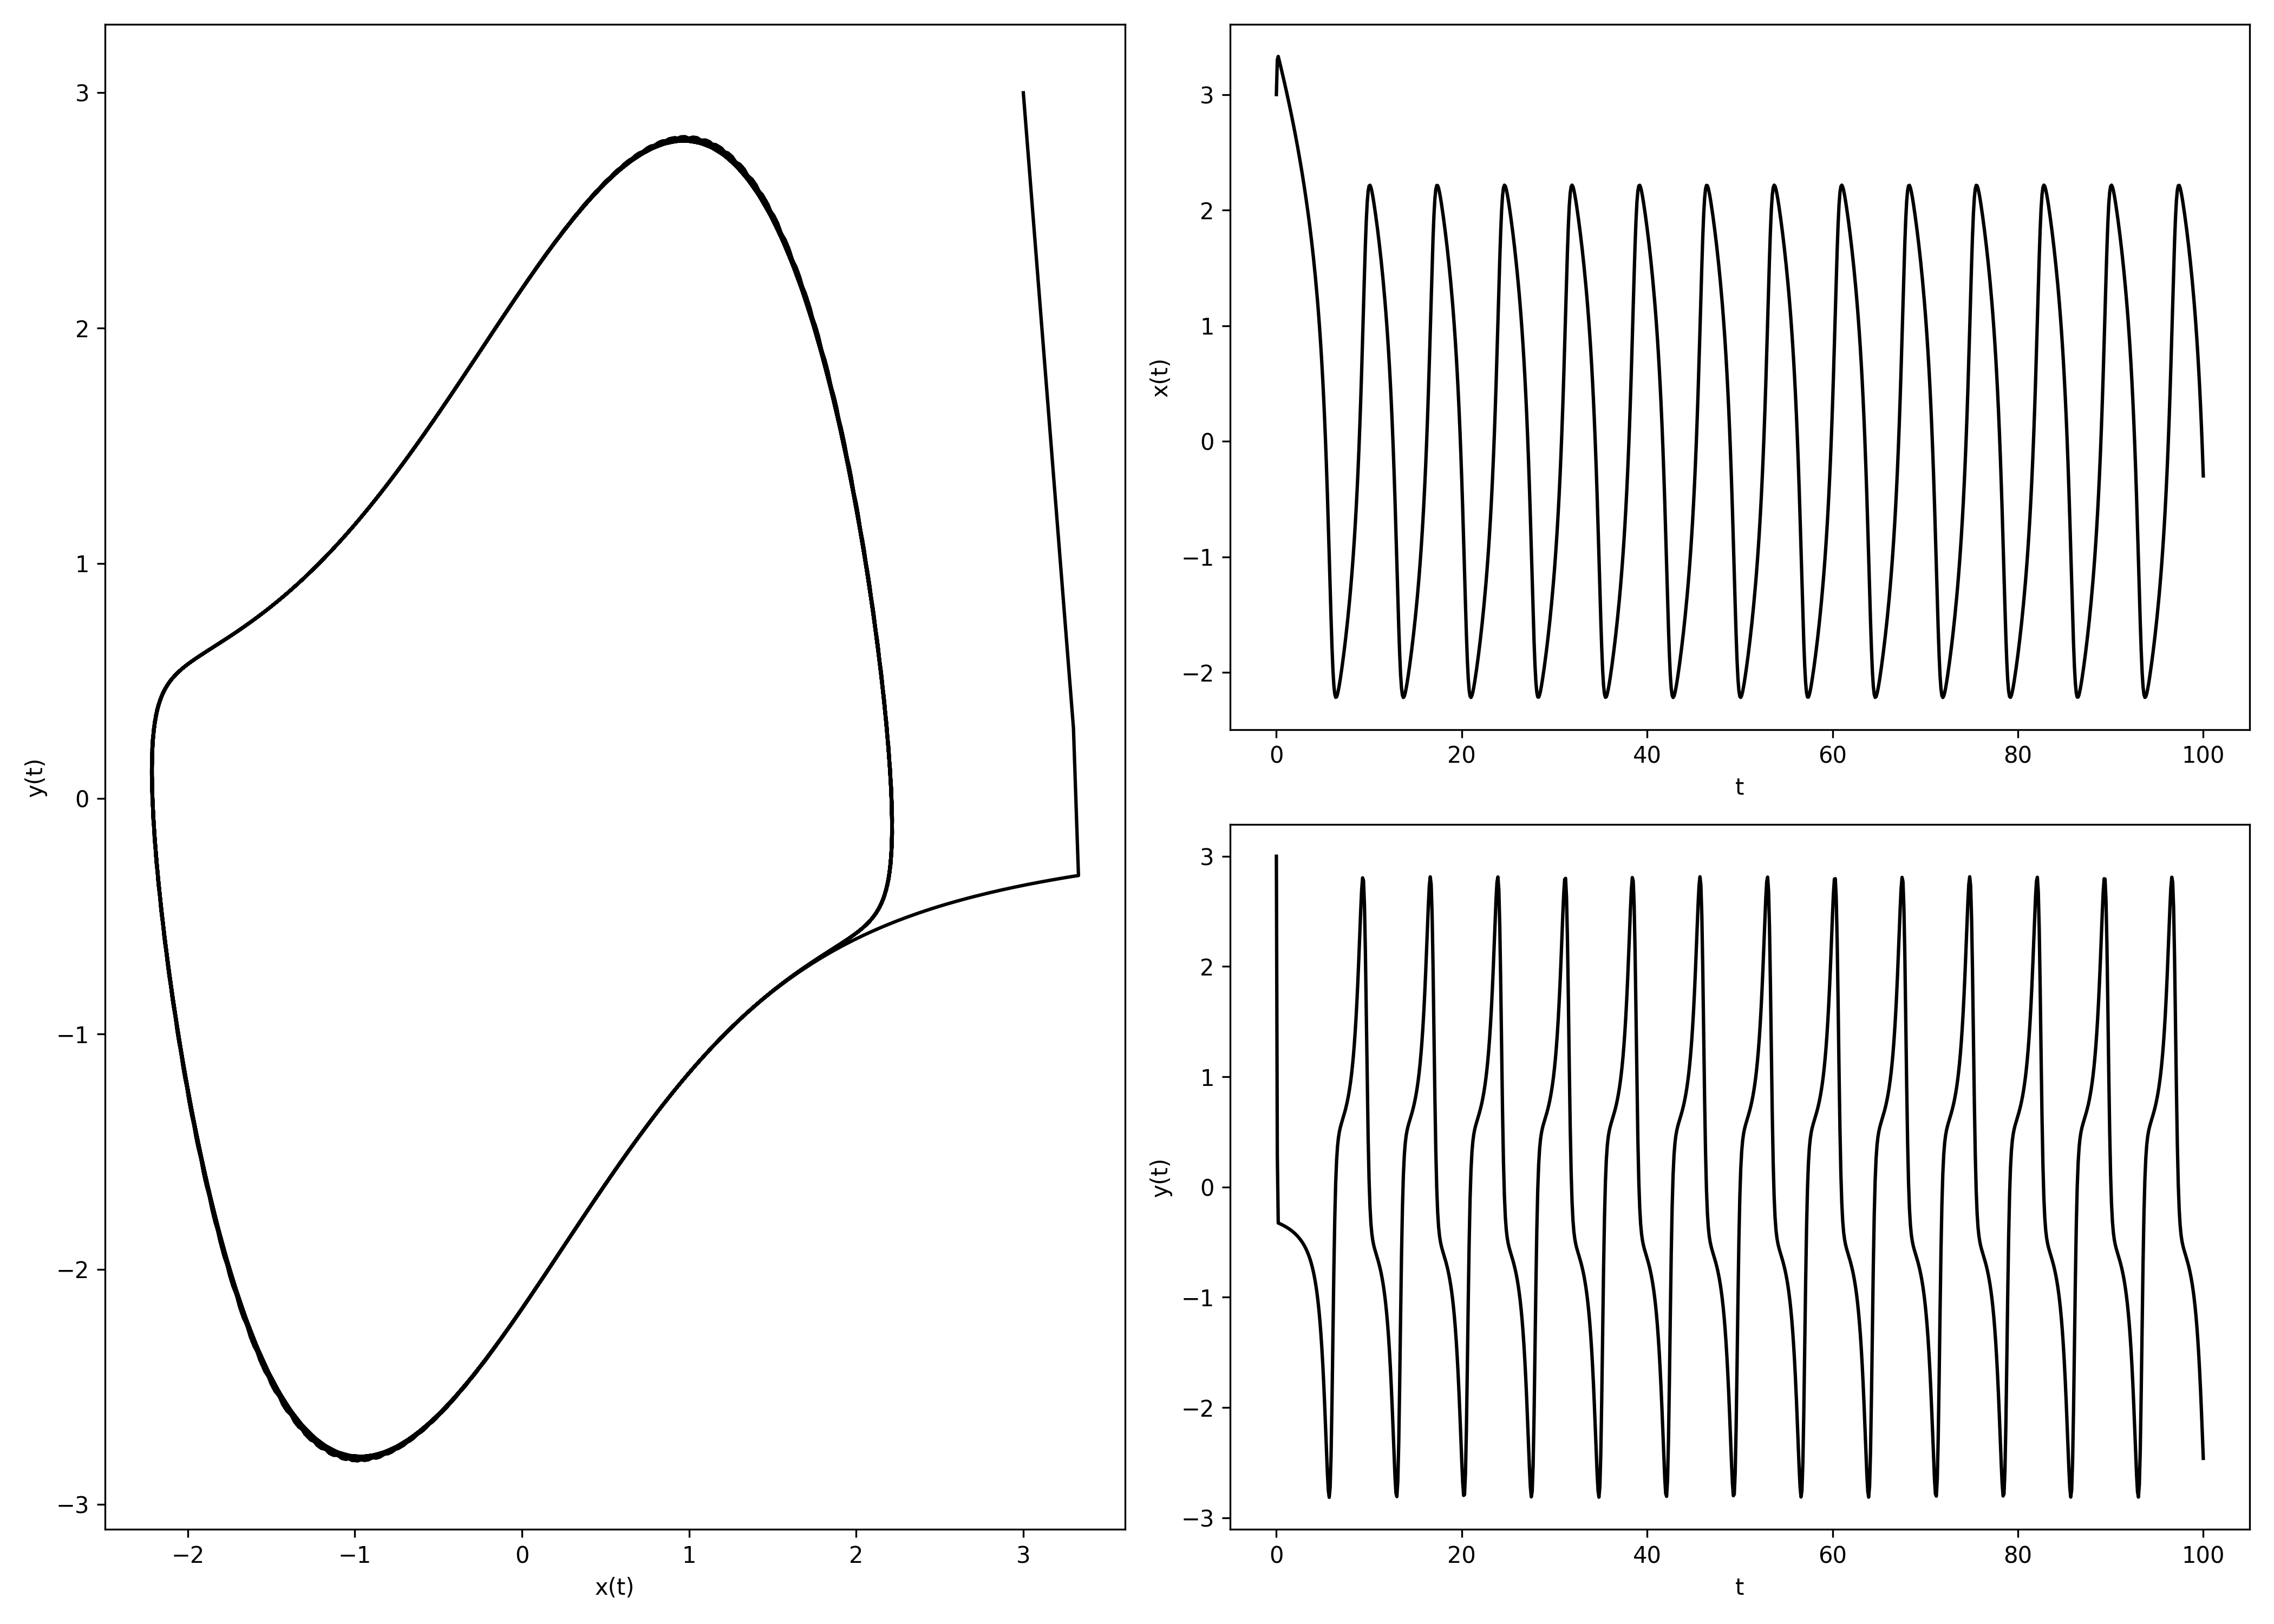
\includegraphics[scale=0.33]{x3,0y3,0mu1,0omega1,0t1,00e+02n1,00e+03.png}
\figcaption{$x_0=3.00, y_0=3.00, \mu=1,00, \omega=1.00, T = 100, N = 1000$}
%N = 2000
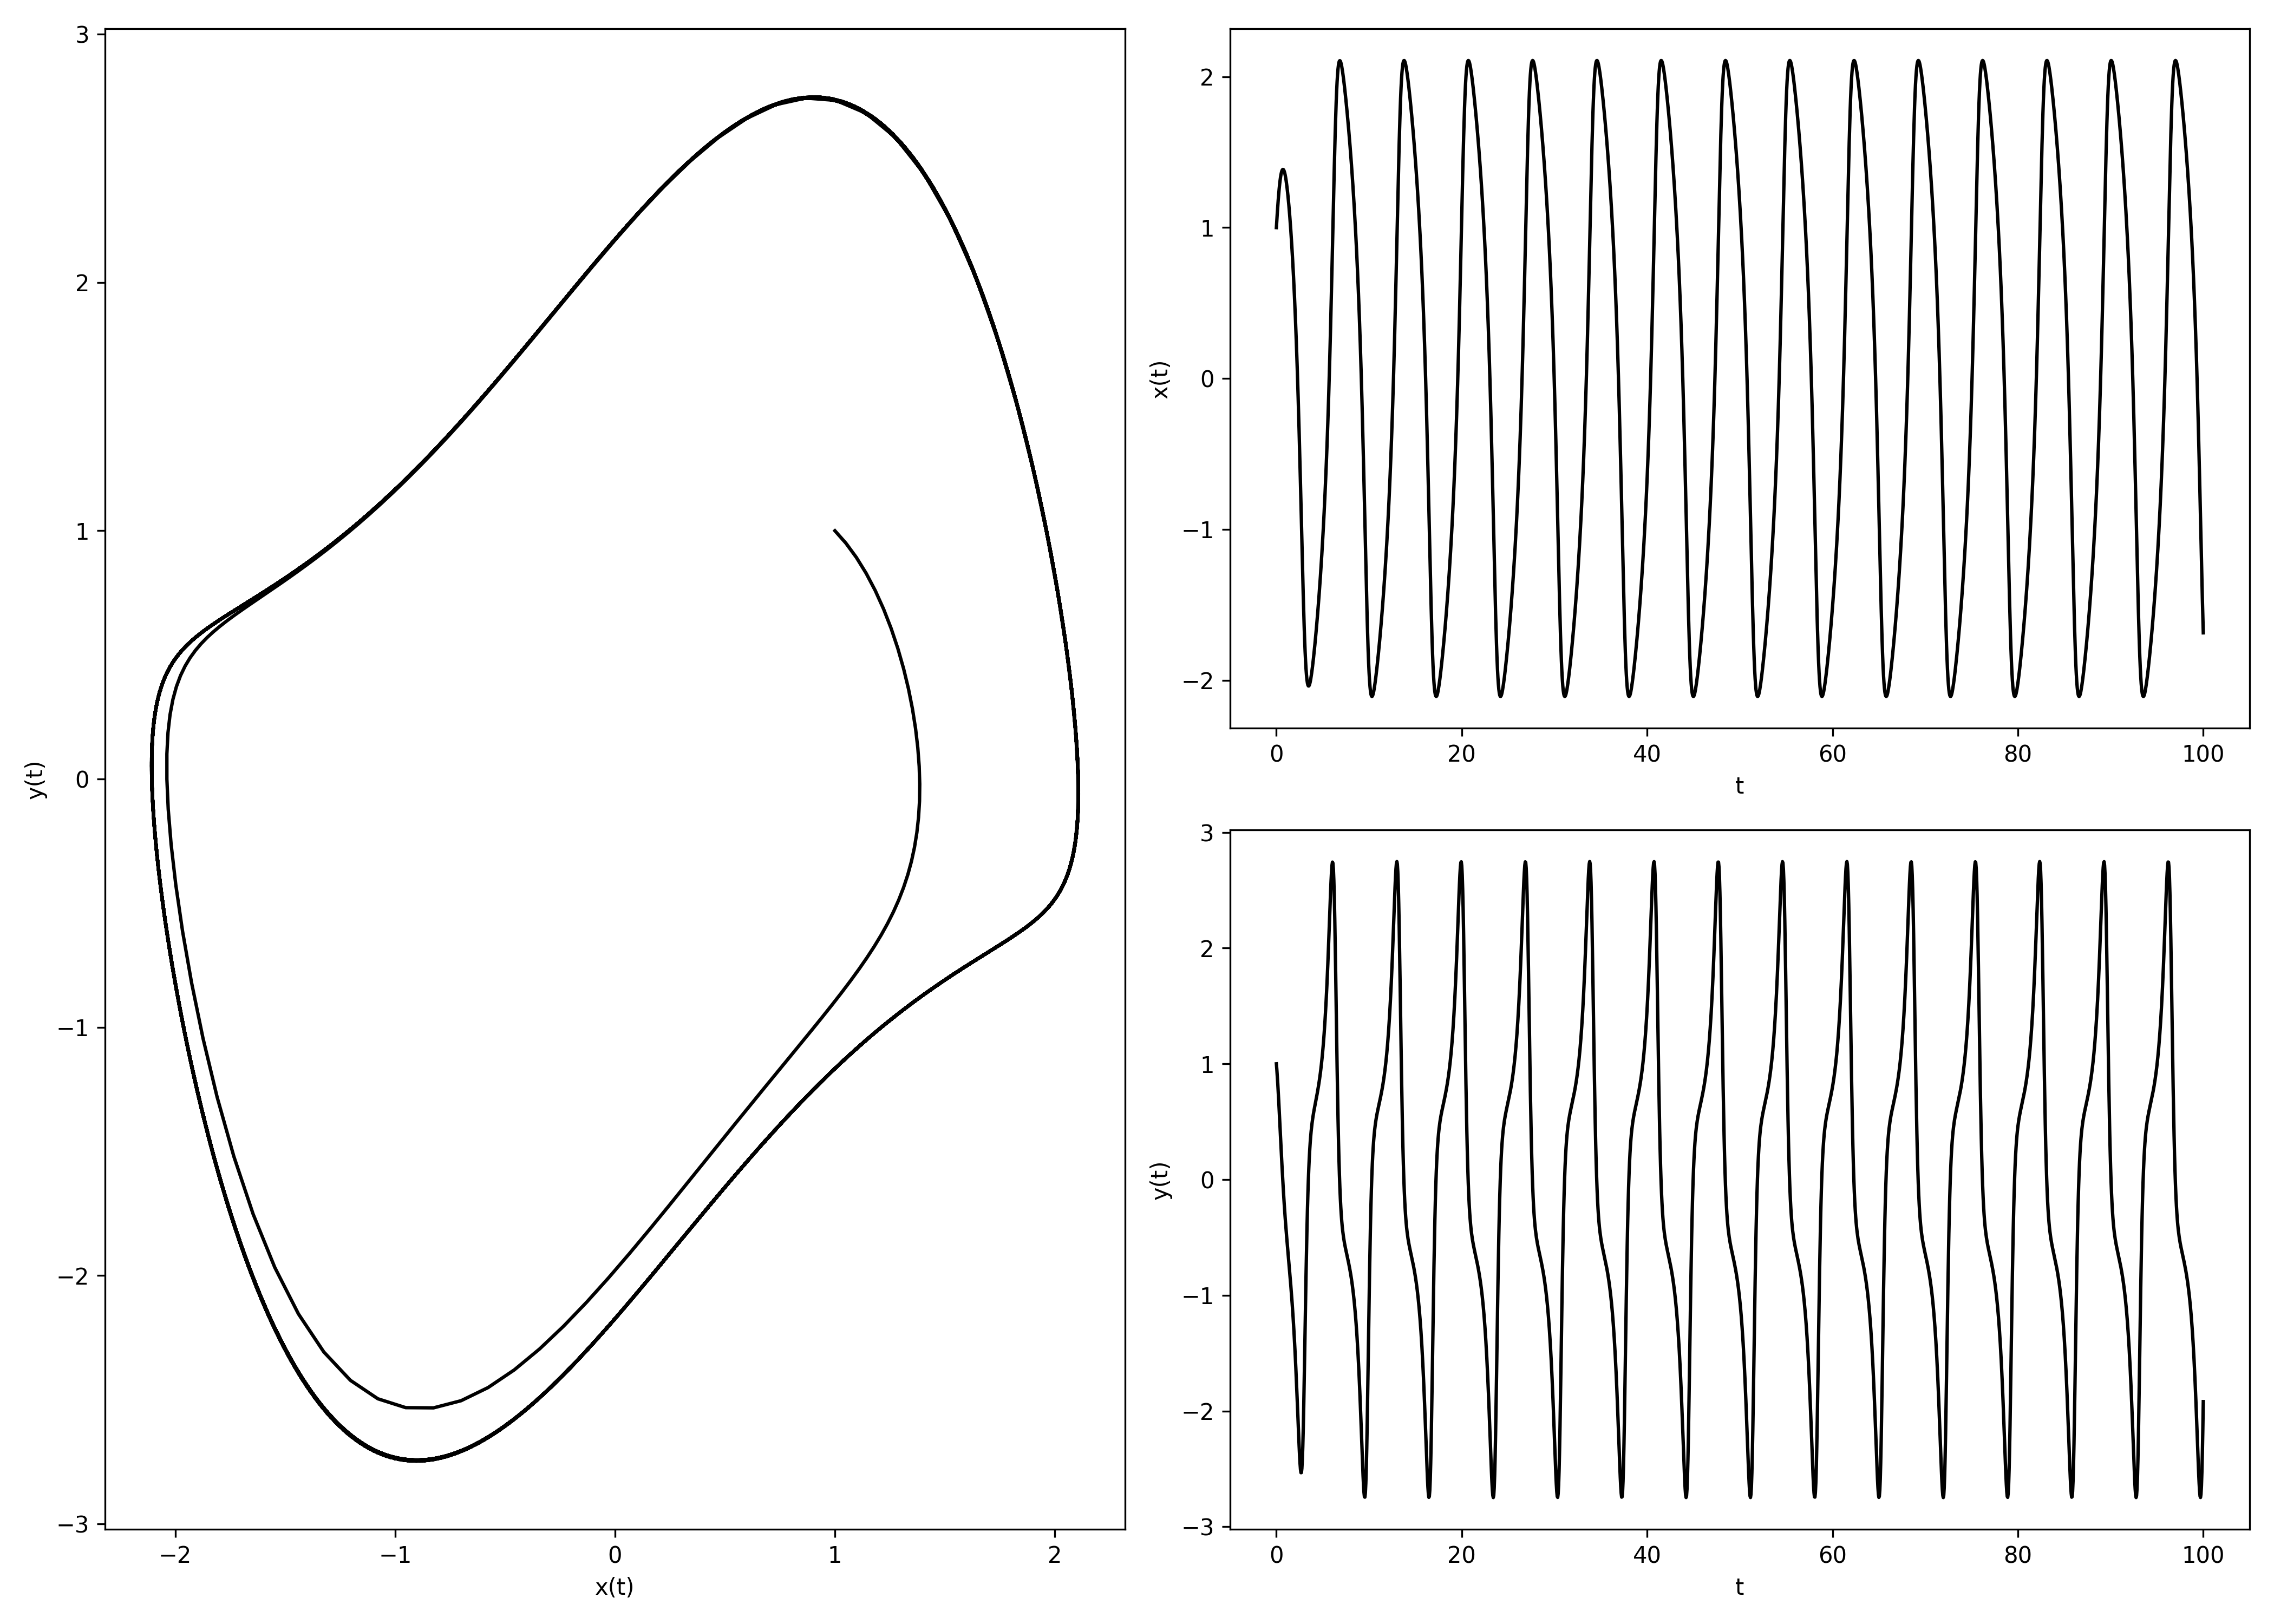
\includegraphics[scale=0.33]{x1,0y1,0mu1,0omega1,0t1,00e+02n2,00e+03.png}
\figcaption{$x_0=1,00, y_0=1.00, \mu=1.00, \omega=1.00, T = 100, N = 2000$}
%パラメーターmu
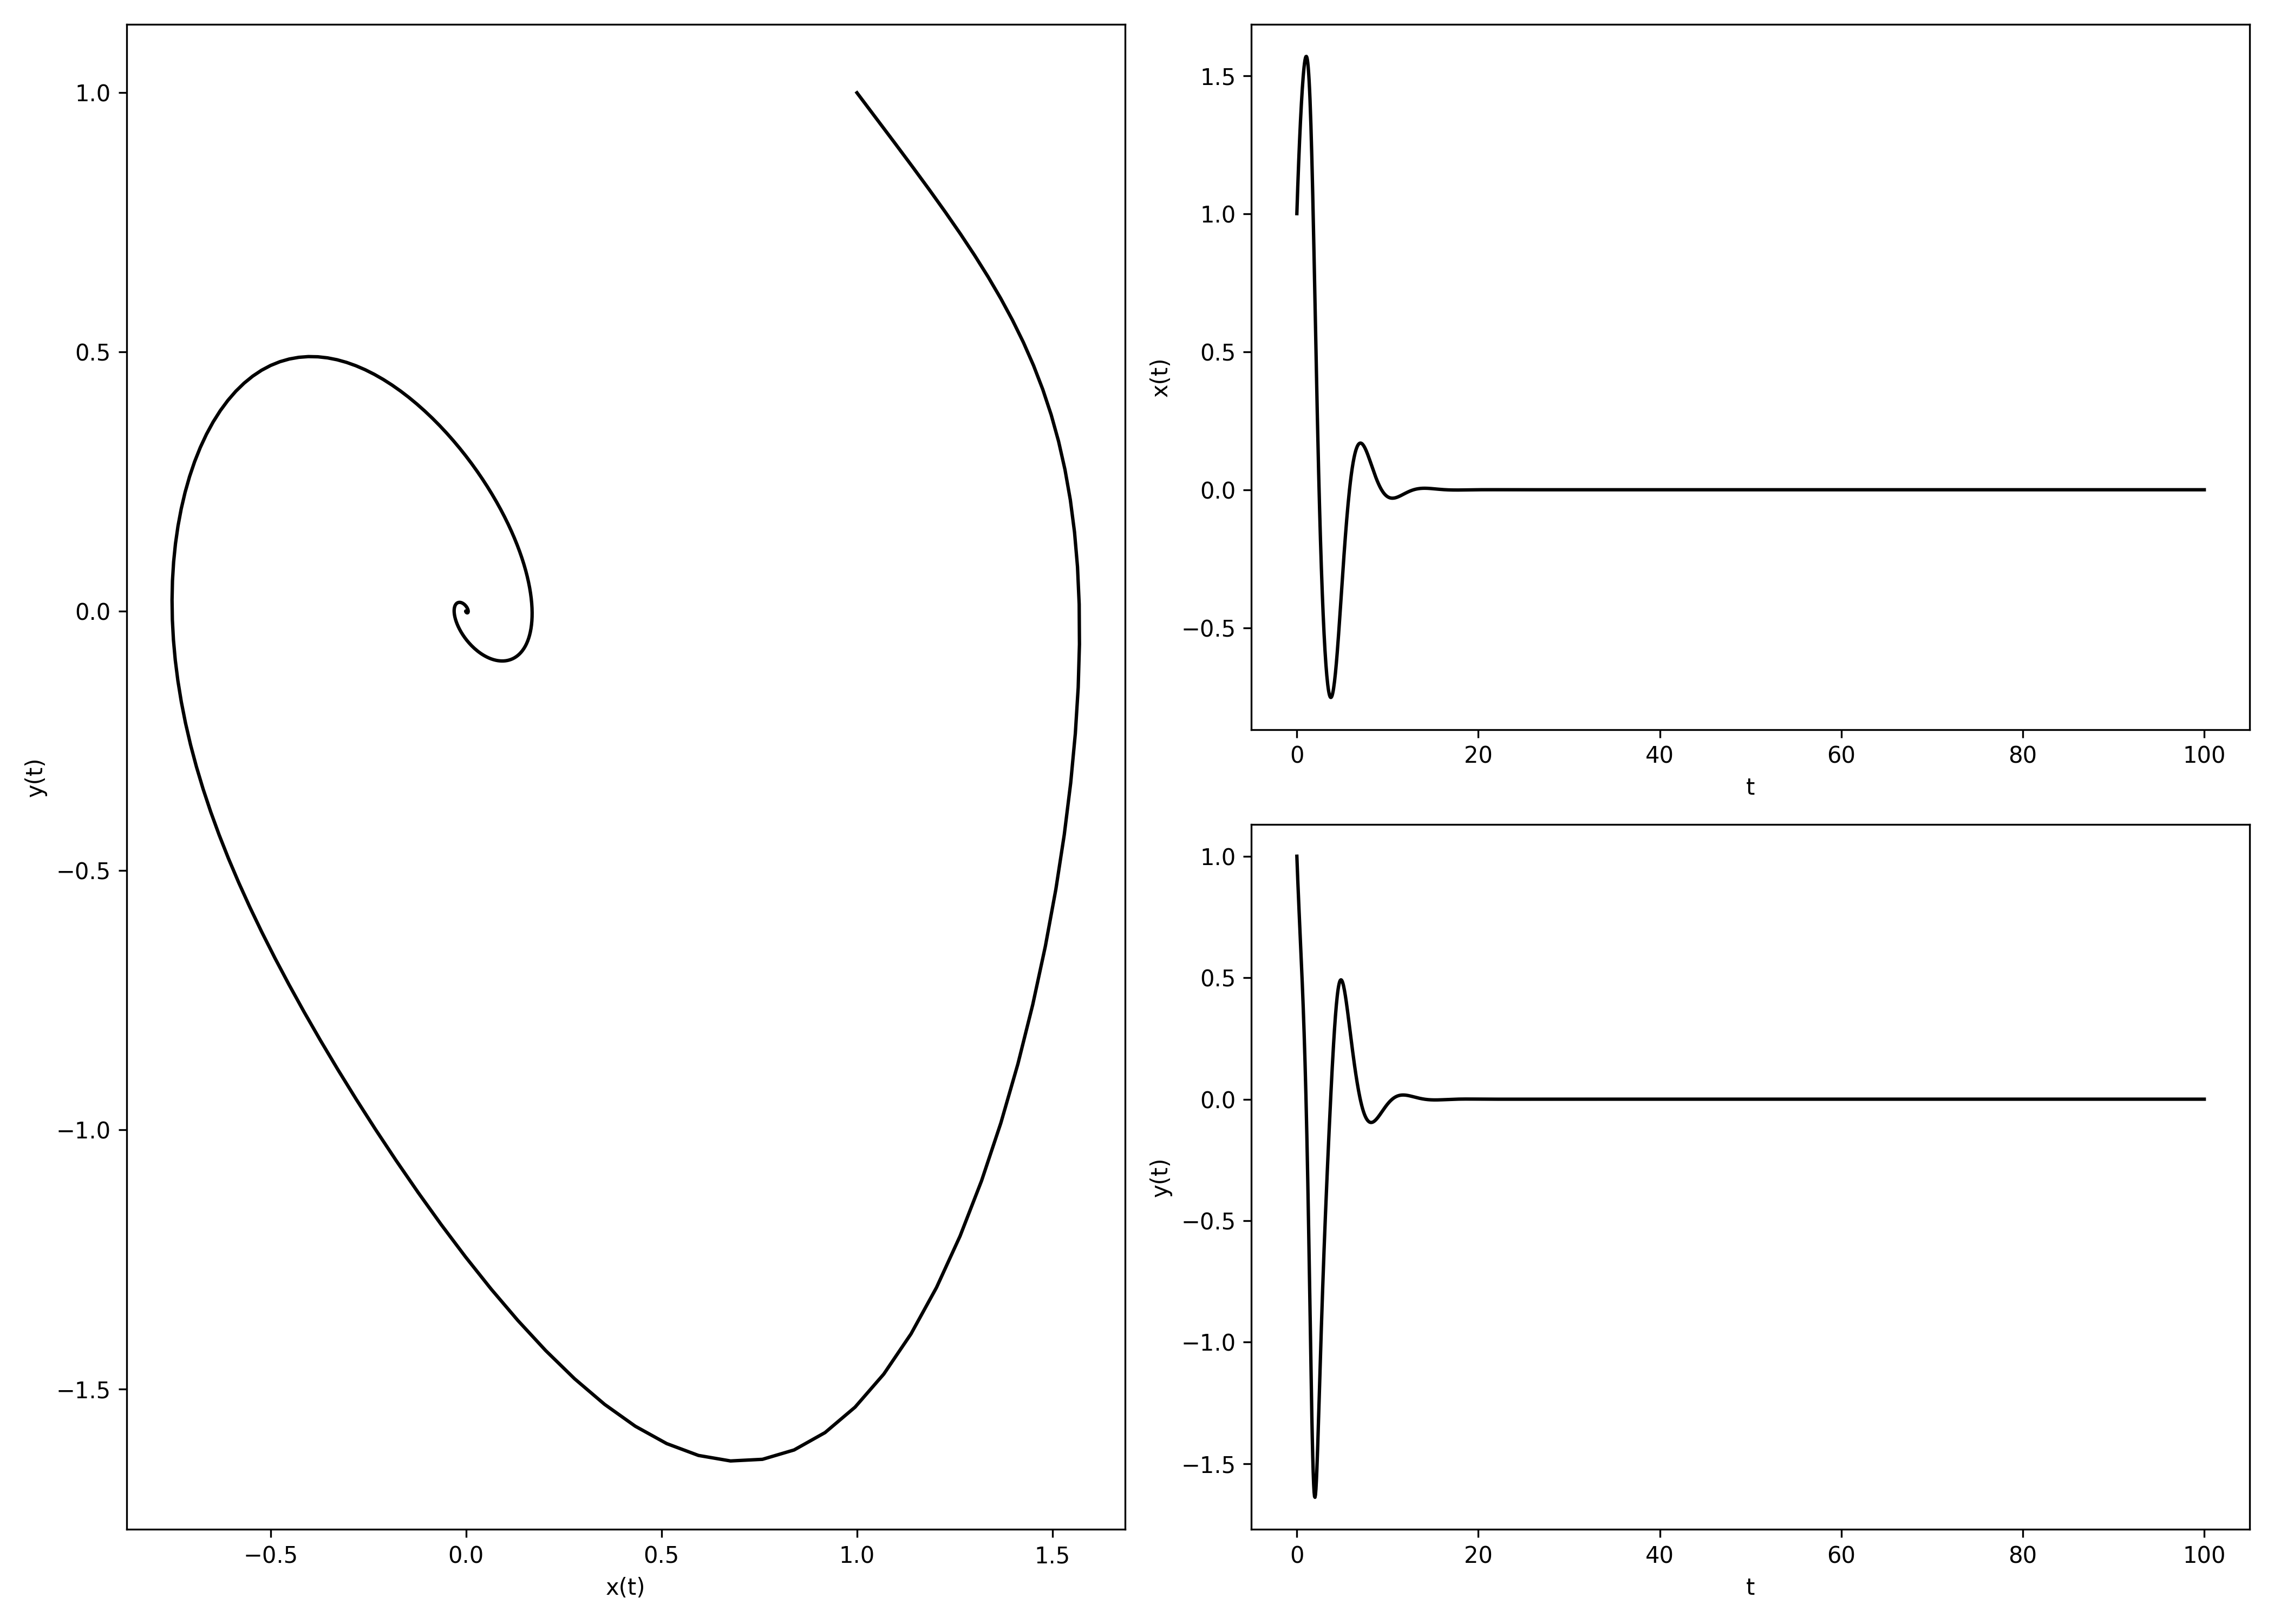
\includegraphics[scale=0.33]{x1,0y1,0mu-1,0omega1,0t1,00e+02n2,00e+03.png}
\figcaption{$x_0=1,00, y_0=1.00, \mu=-1.00, \omega=1.00, T = 100, N = 2000$}
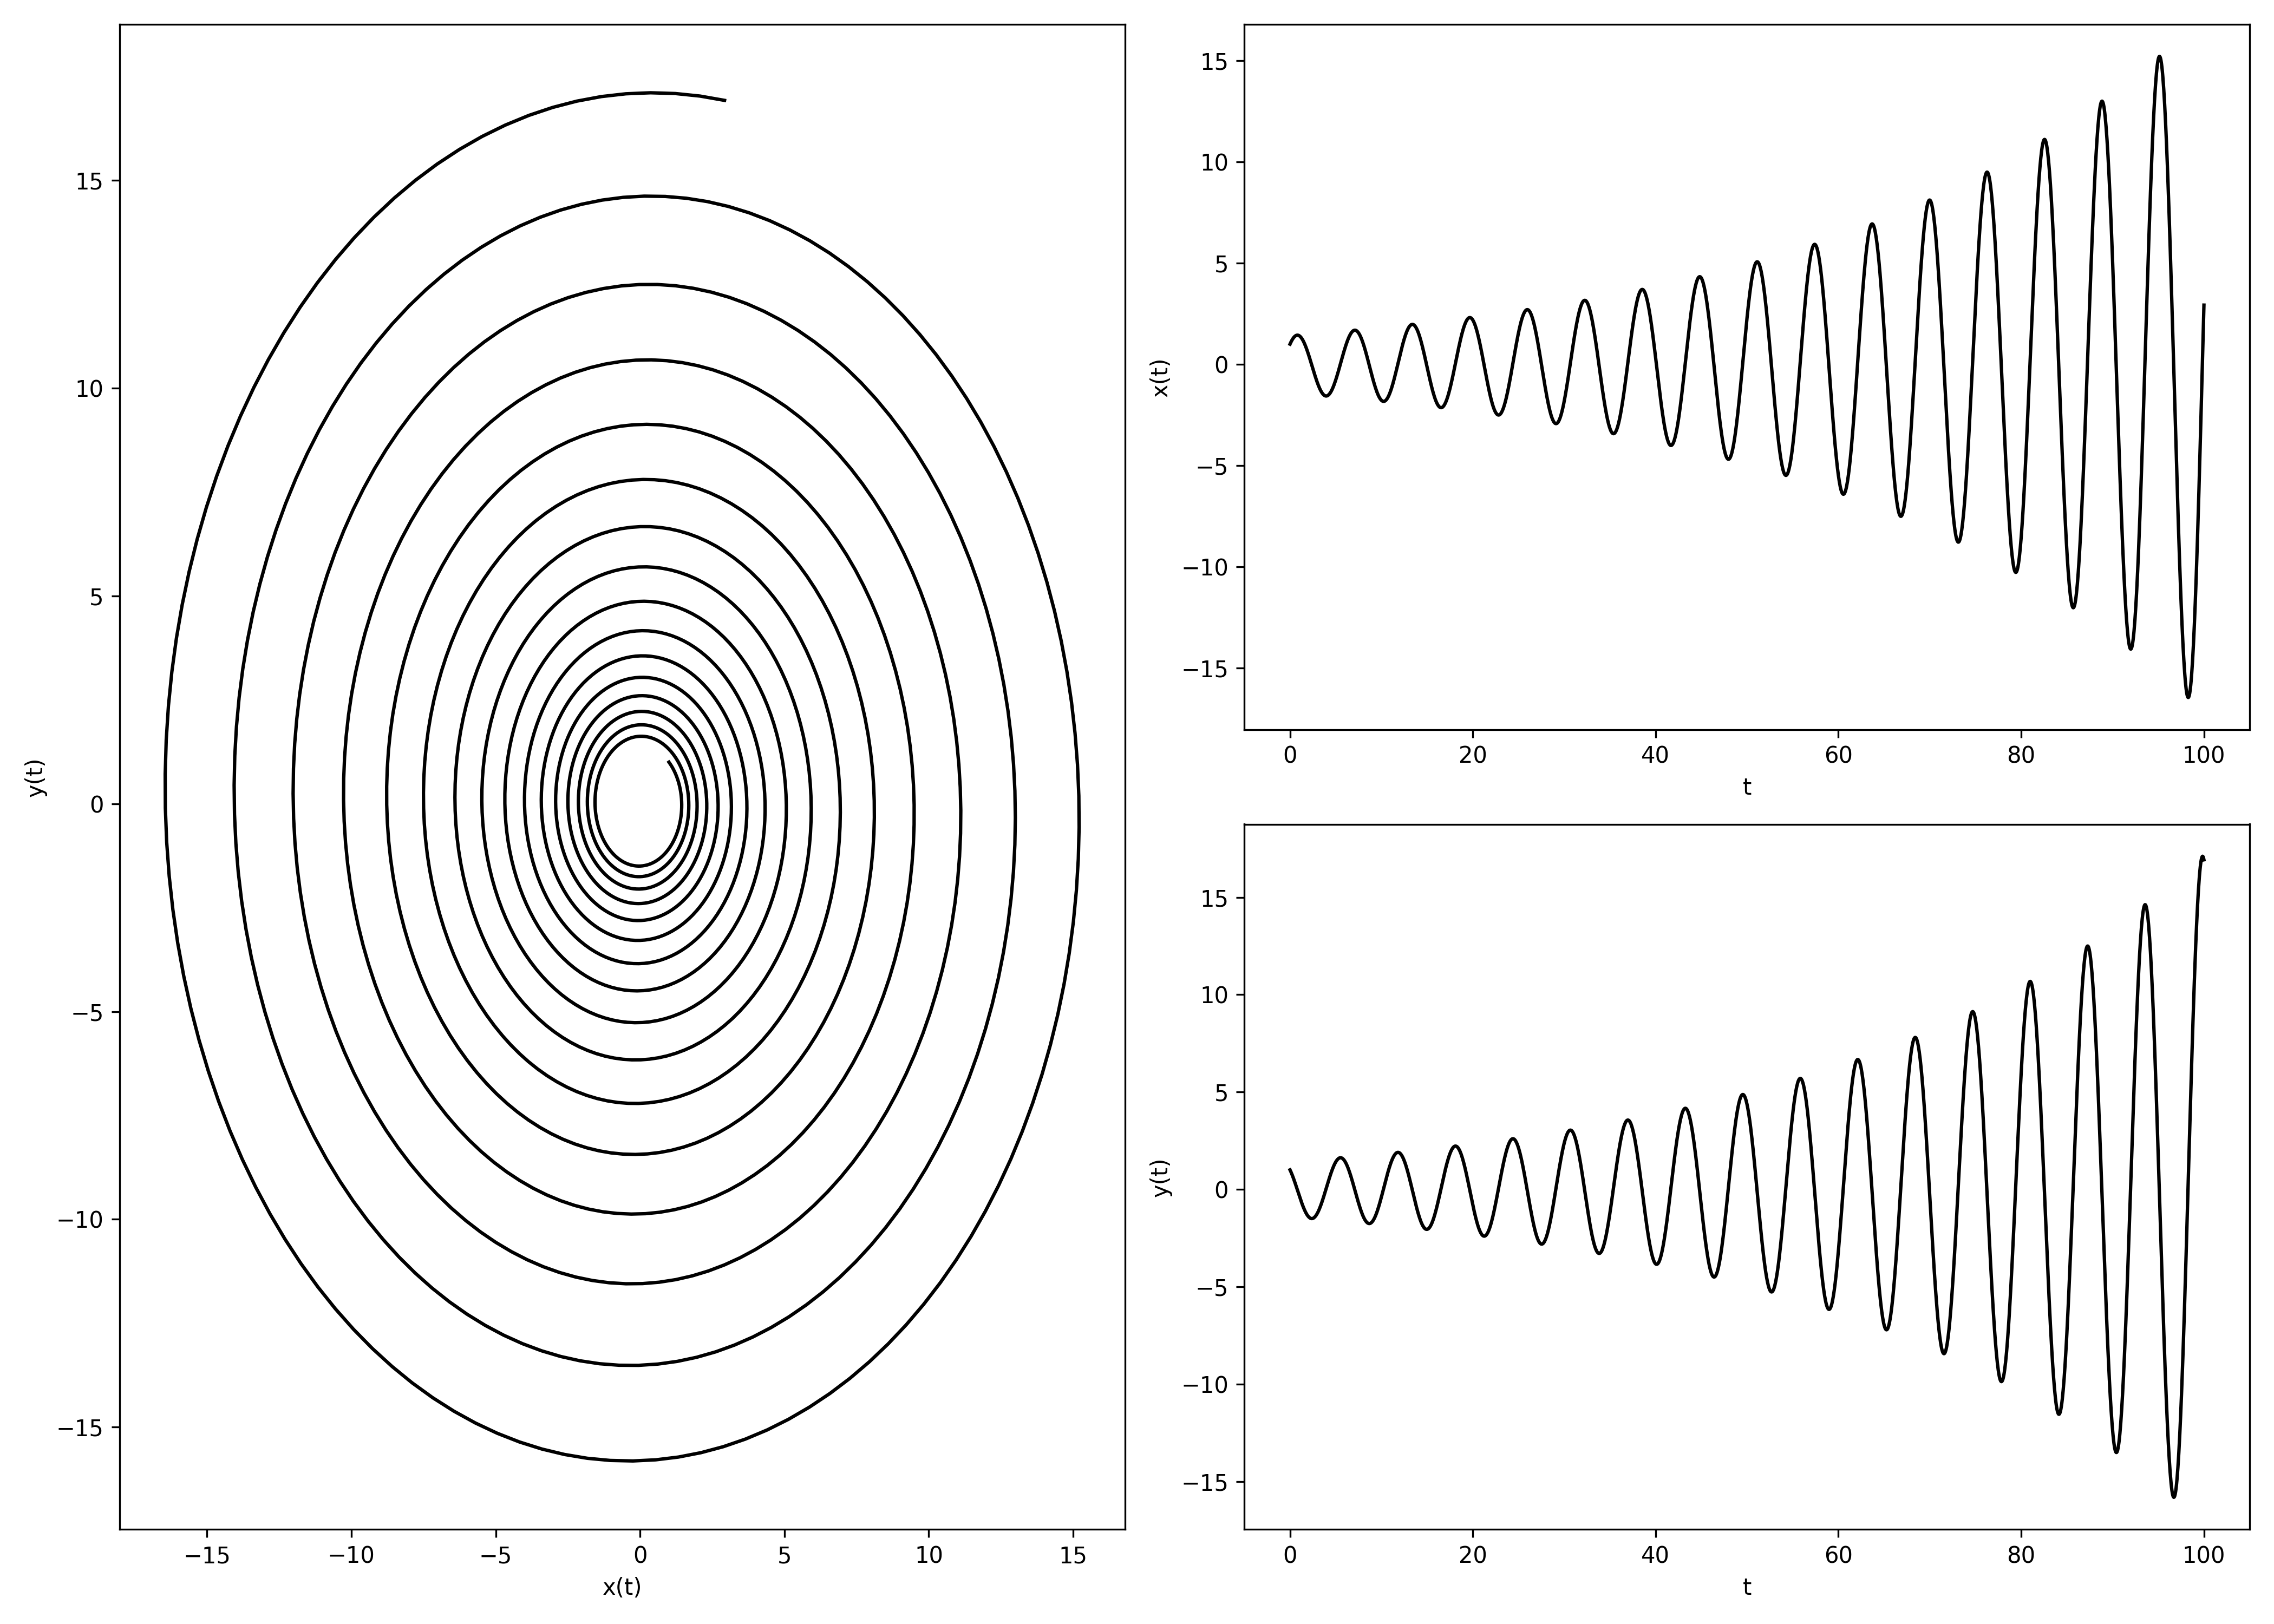
\includegraphics[scale=0.33]{x1,0y1,0mu0,0omega1,0t1,00e+02n2,00e+03.png}
\figcaption{$x_0=1,00, y_0=1.00, \mu=0.00, \omega=1.00, T = 100, N = 2000$}
% 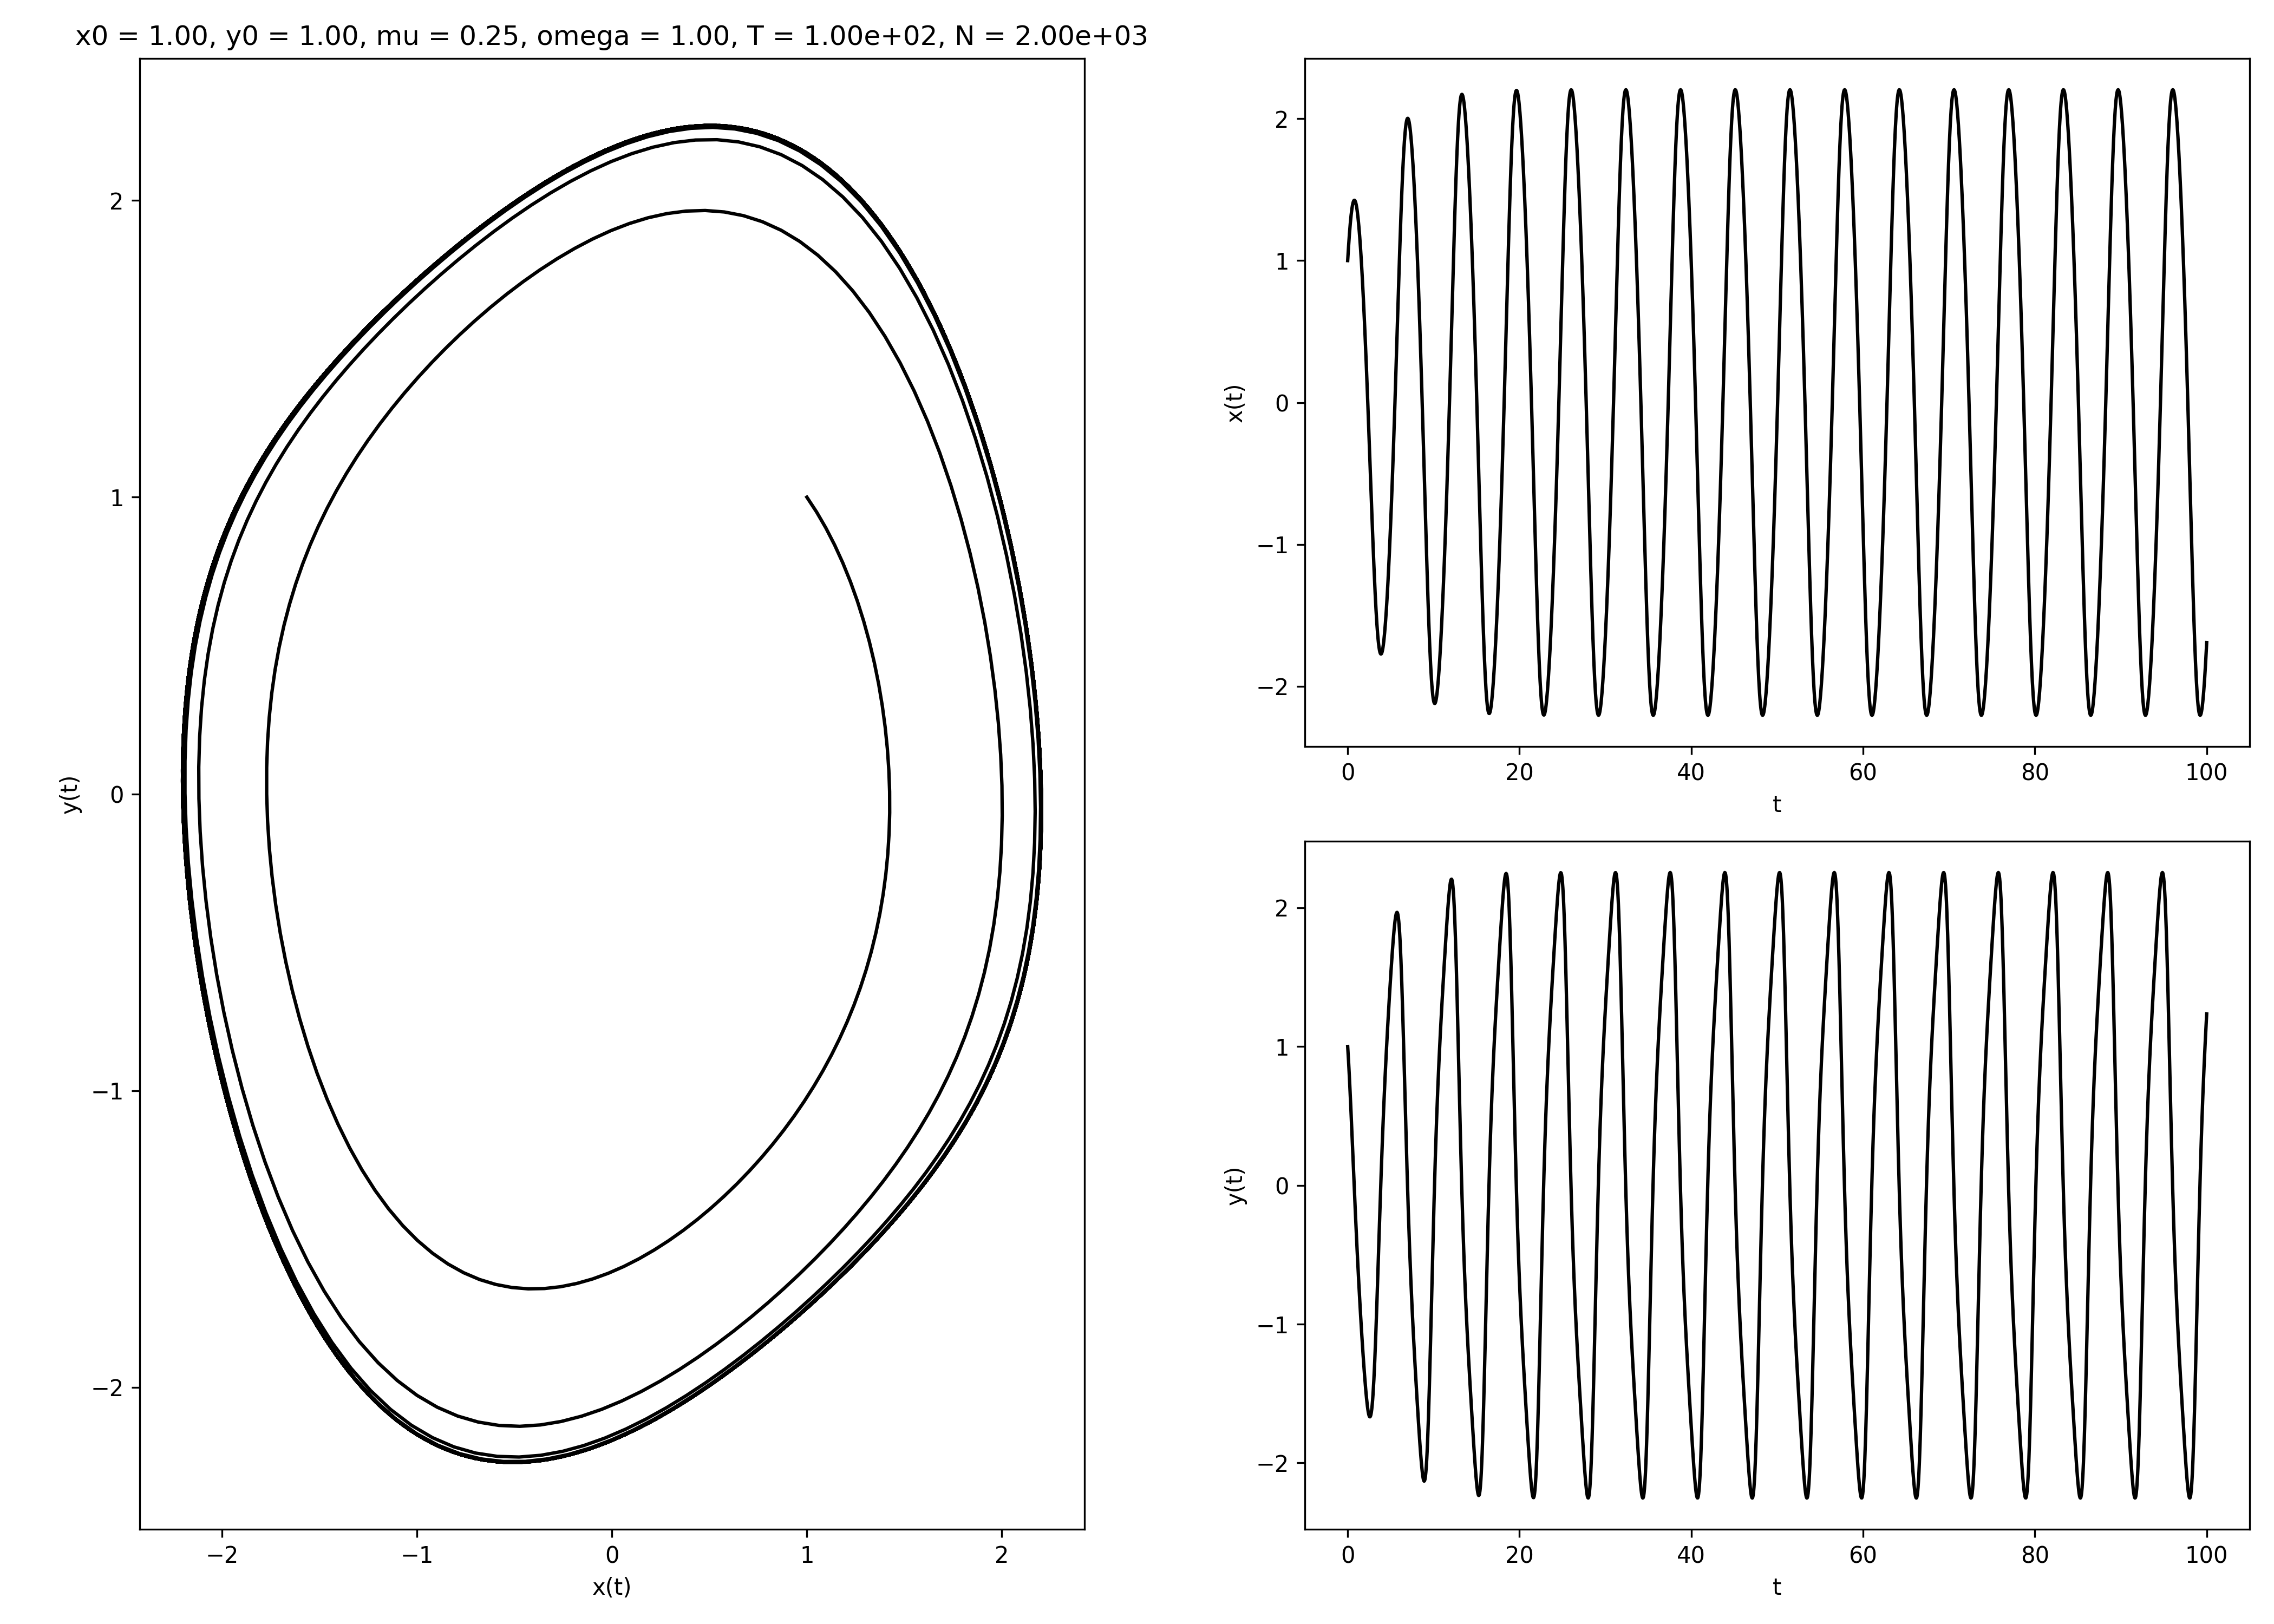
\includegraphics[scale=0.33]{x1,0y1,0mu0,2omega1,0t1,00e+02n2,00e+03.png}
% \figcaption{$x_0=1,00, y_0=1.00, \mu=0.25, \omega=1.00, T = 200, N = 2000$}
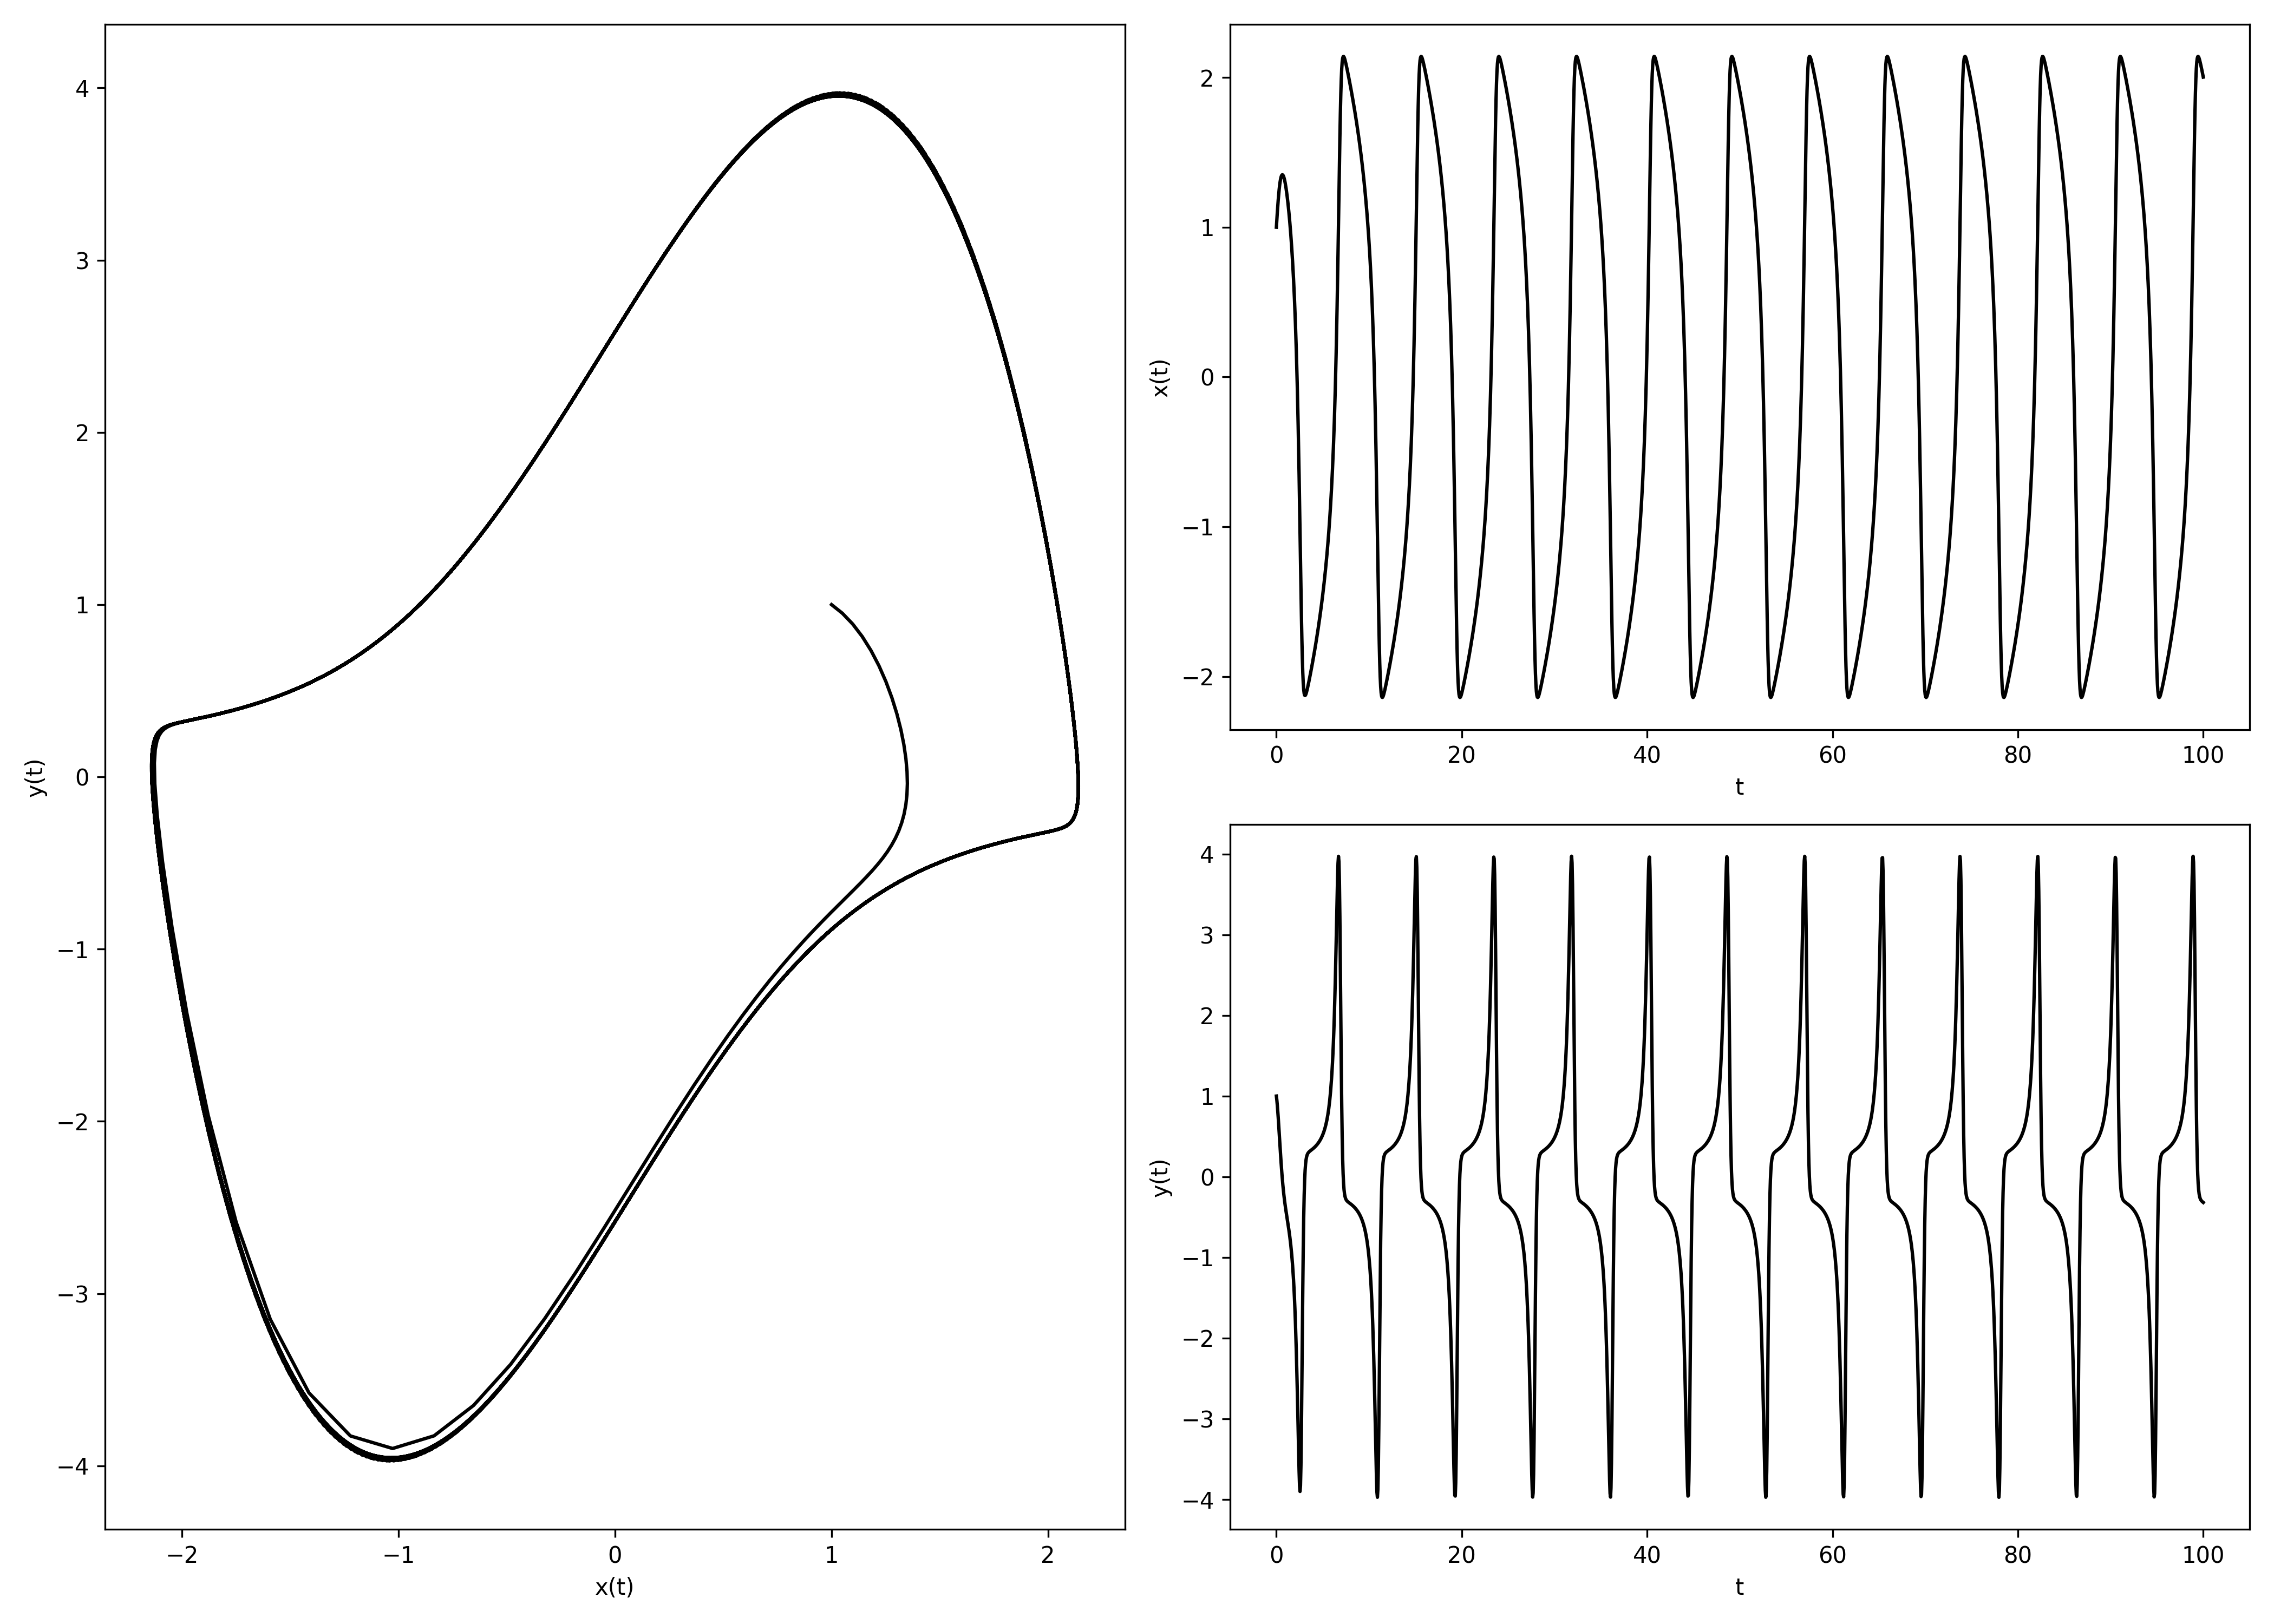
\includegraphics[scale=0.33]{x1,0y1,0mu2,0omega1,0t1,00e+02n2,00e+03.png}
\figcaption{$x_0=1,00, y_0=1.00, \mu=2.00, \omega=1.00, T = 100, N = 2000$}
%パラメーターomega
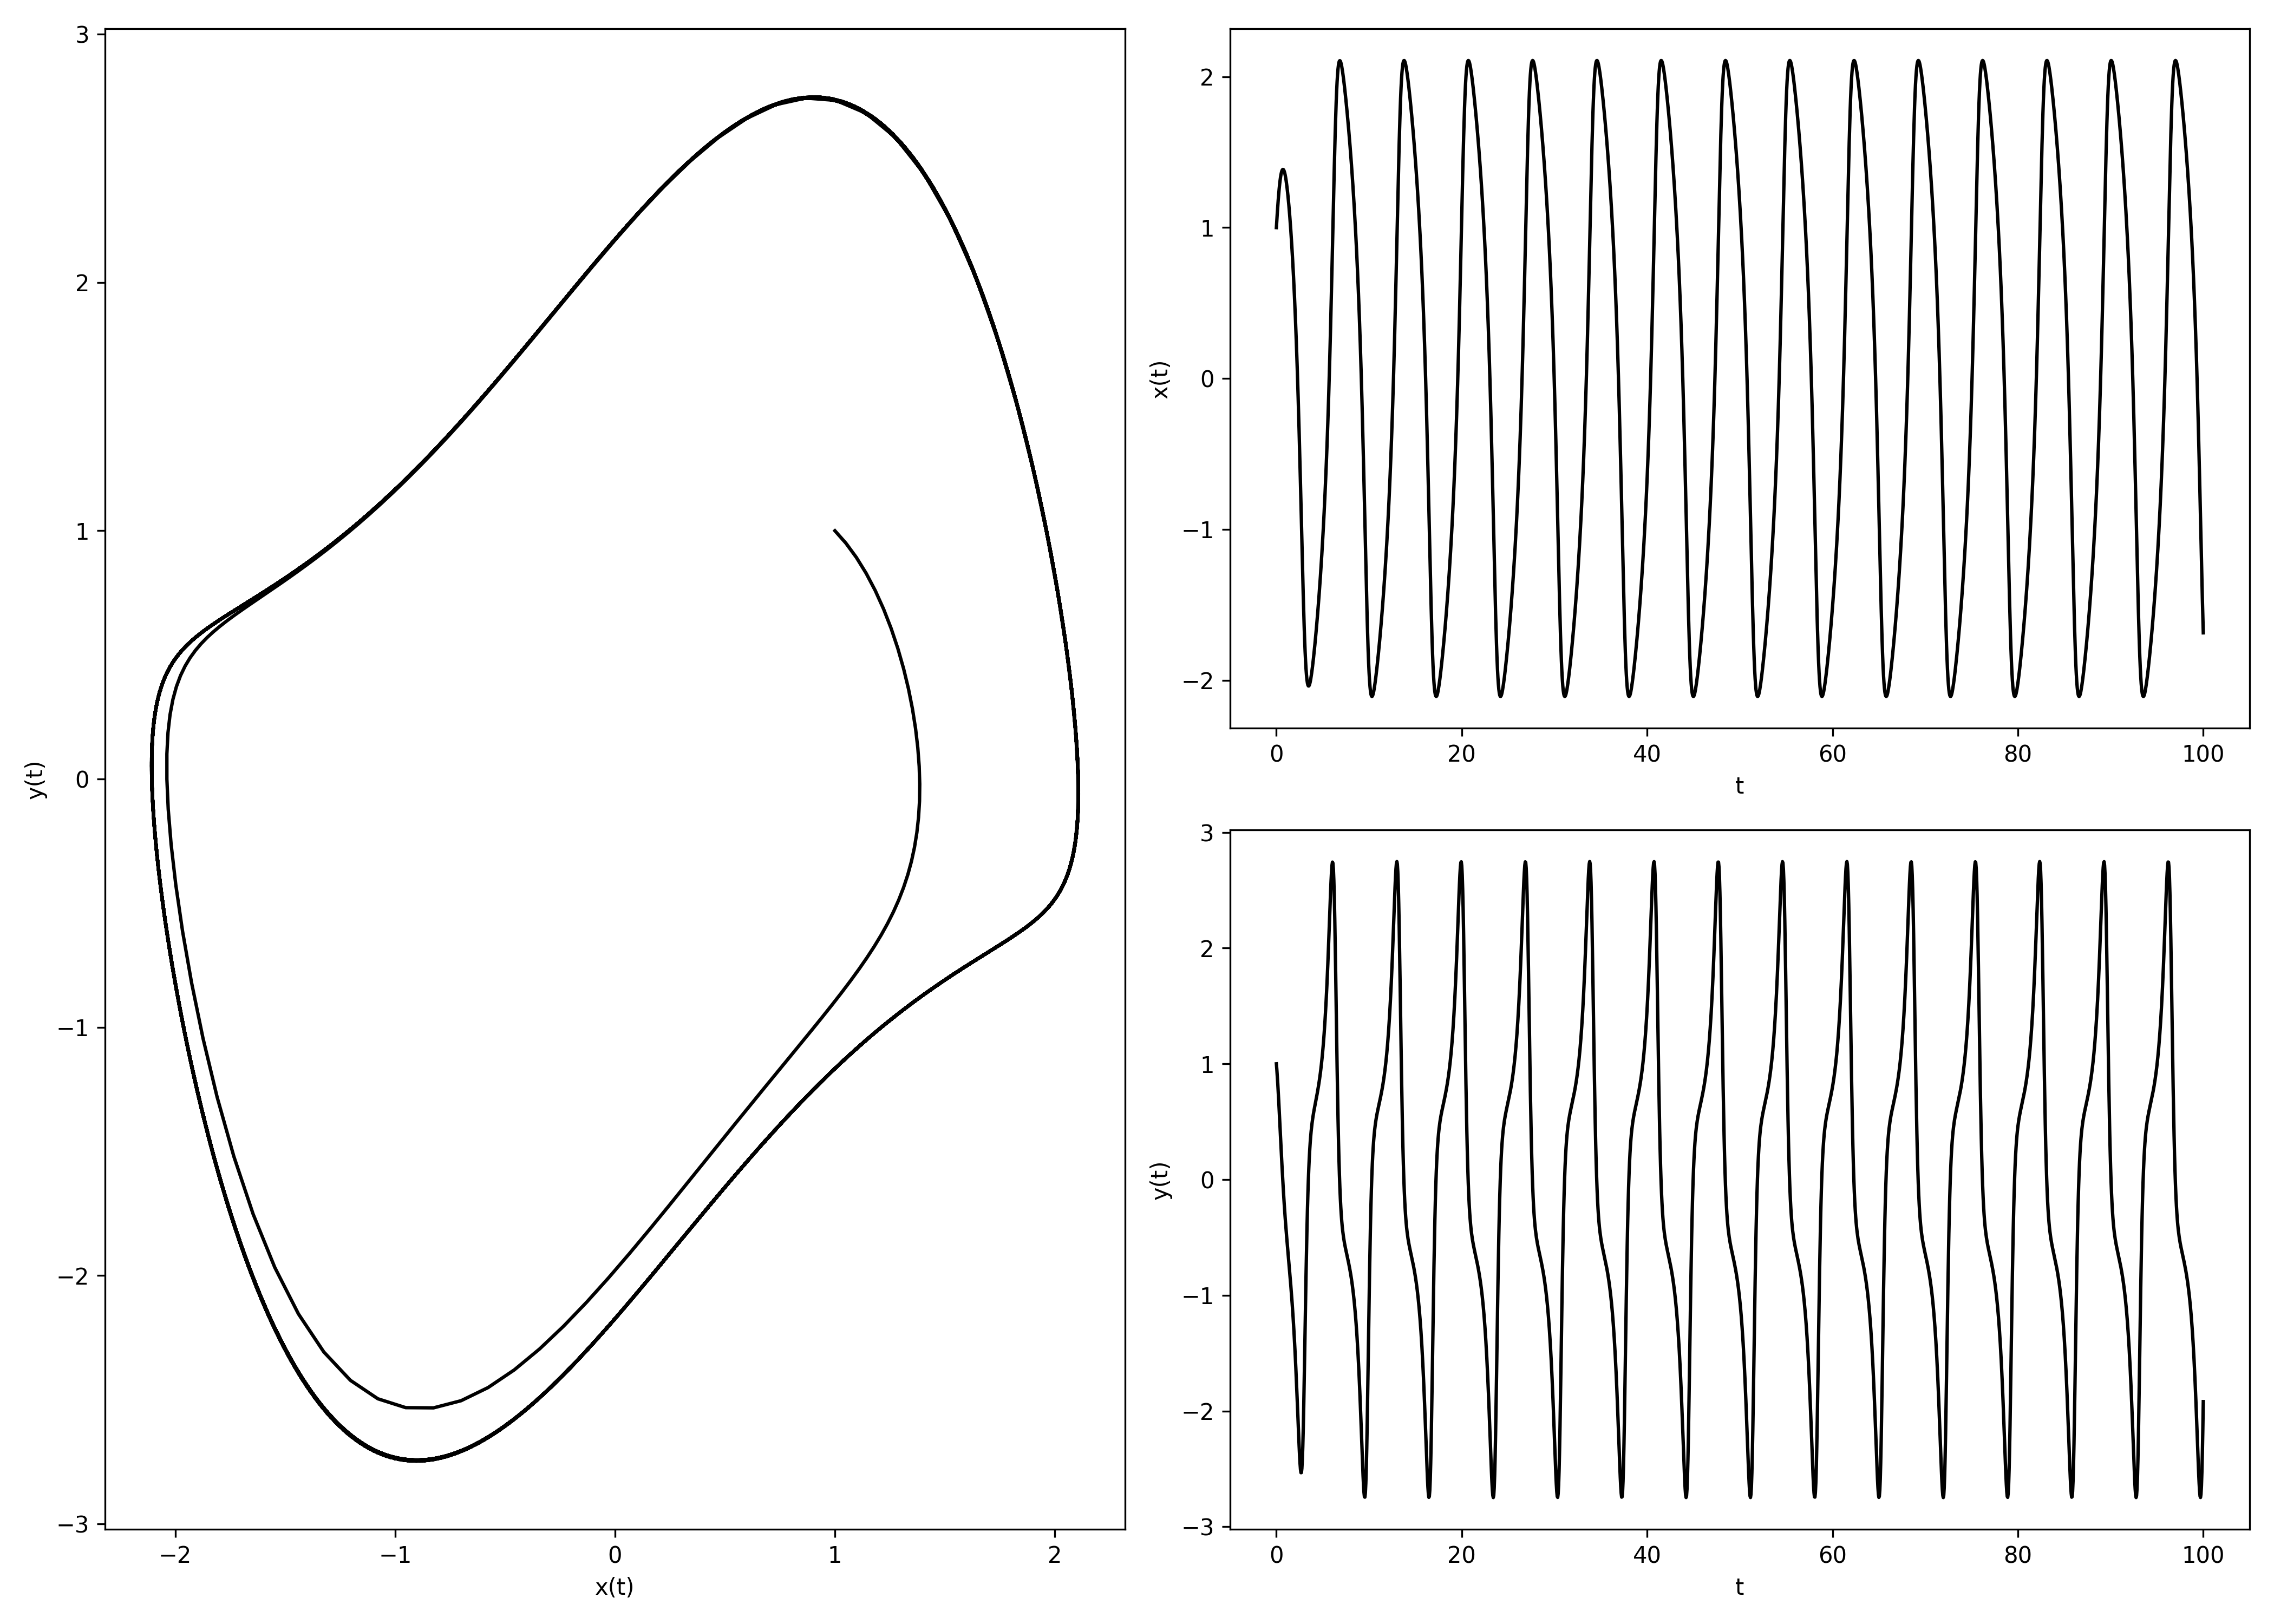
\includegraphics[scale=0.33]{x1,0y1,0mu1,0omega-1,0t1,00e+02n2,00e+03.png}
\figcaption{$x_0=1,00, y_0=1.00, \mu=1.00, \omega=-1.00, T = 200, N = 2000$}
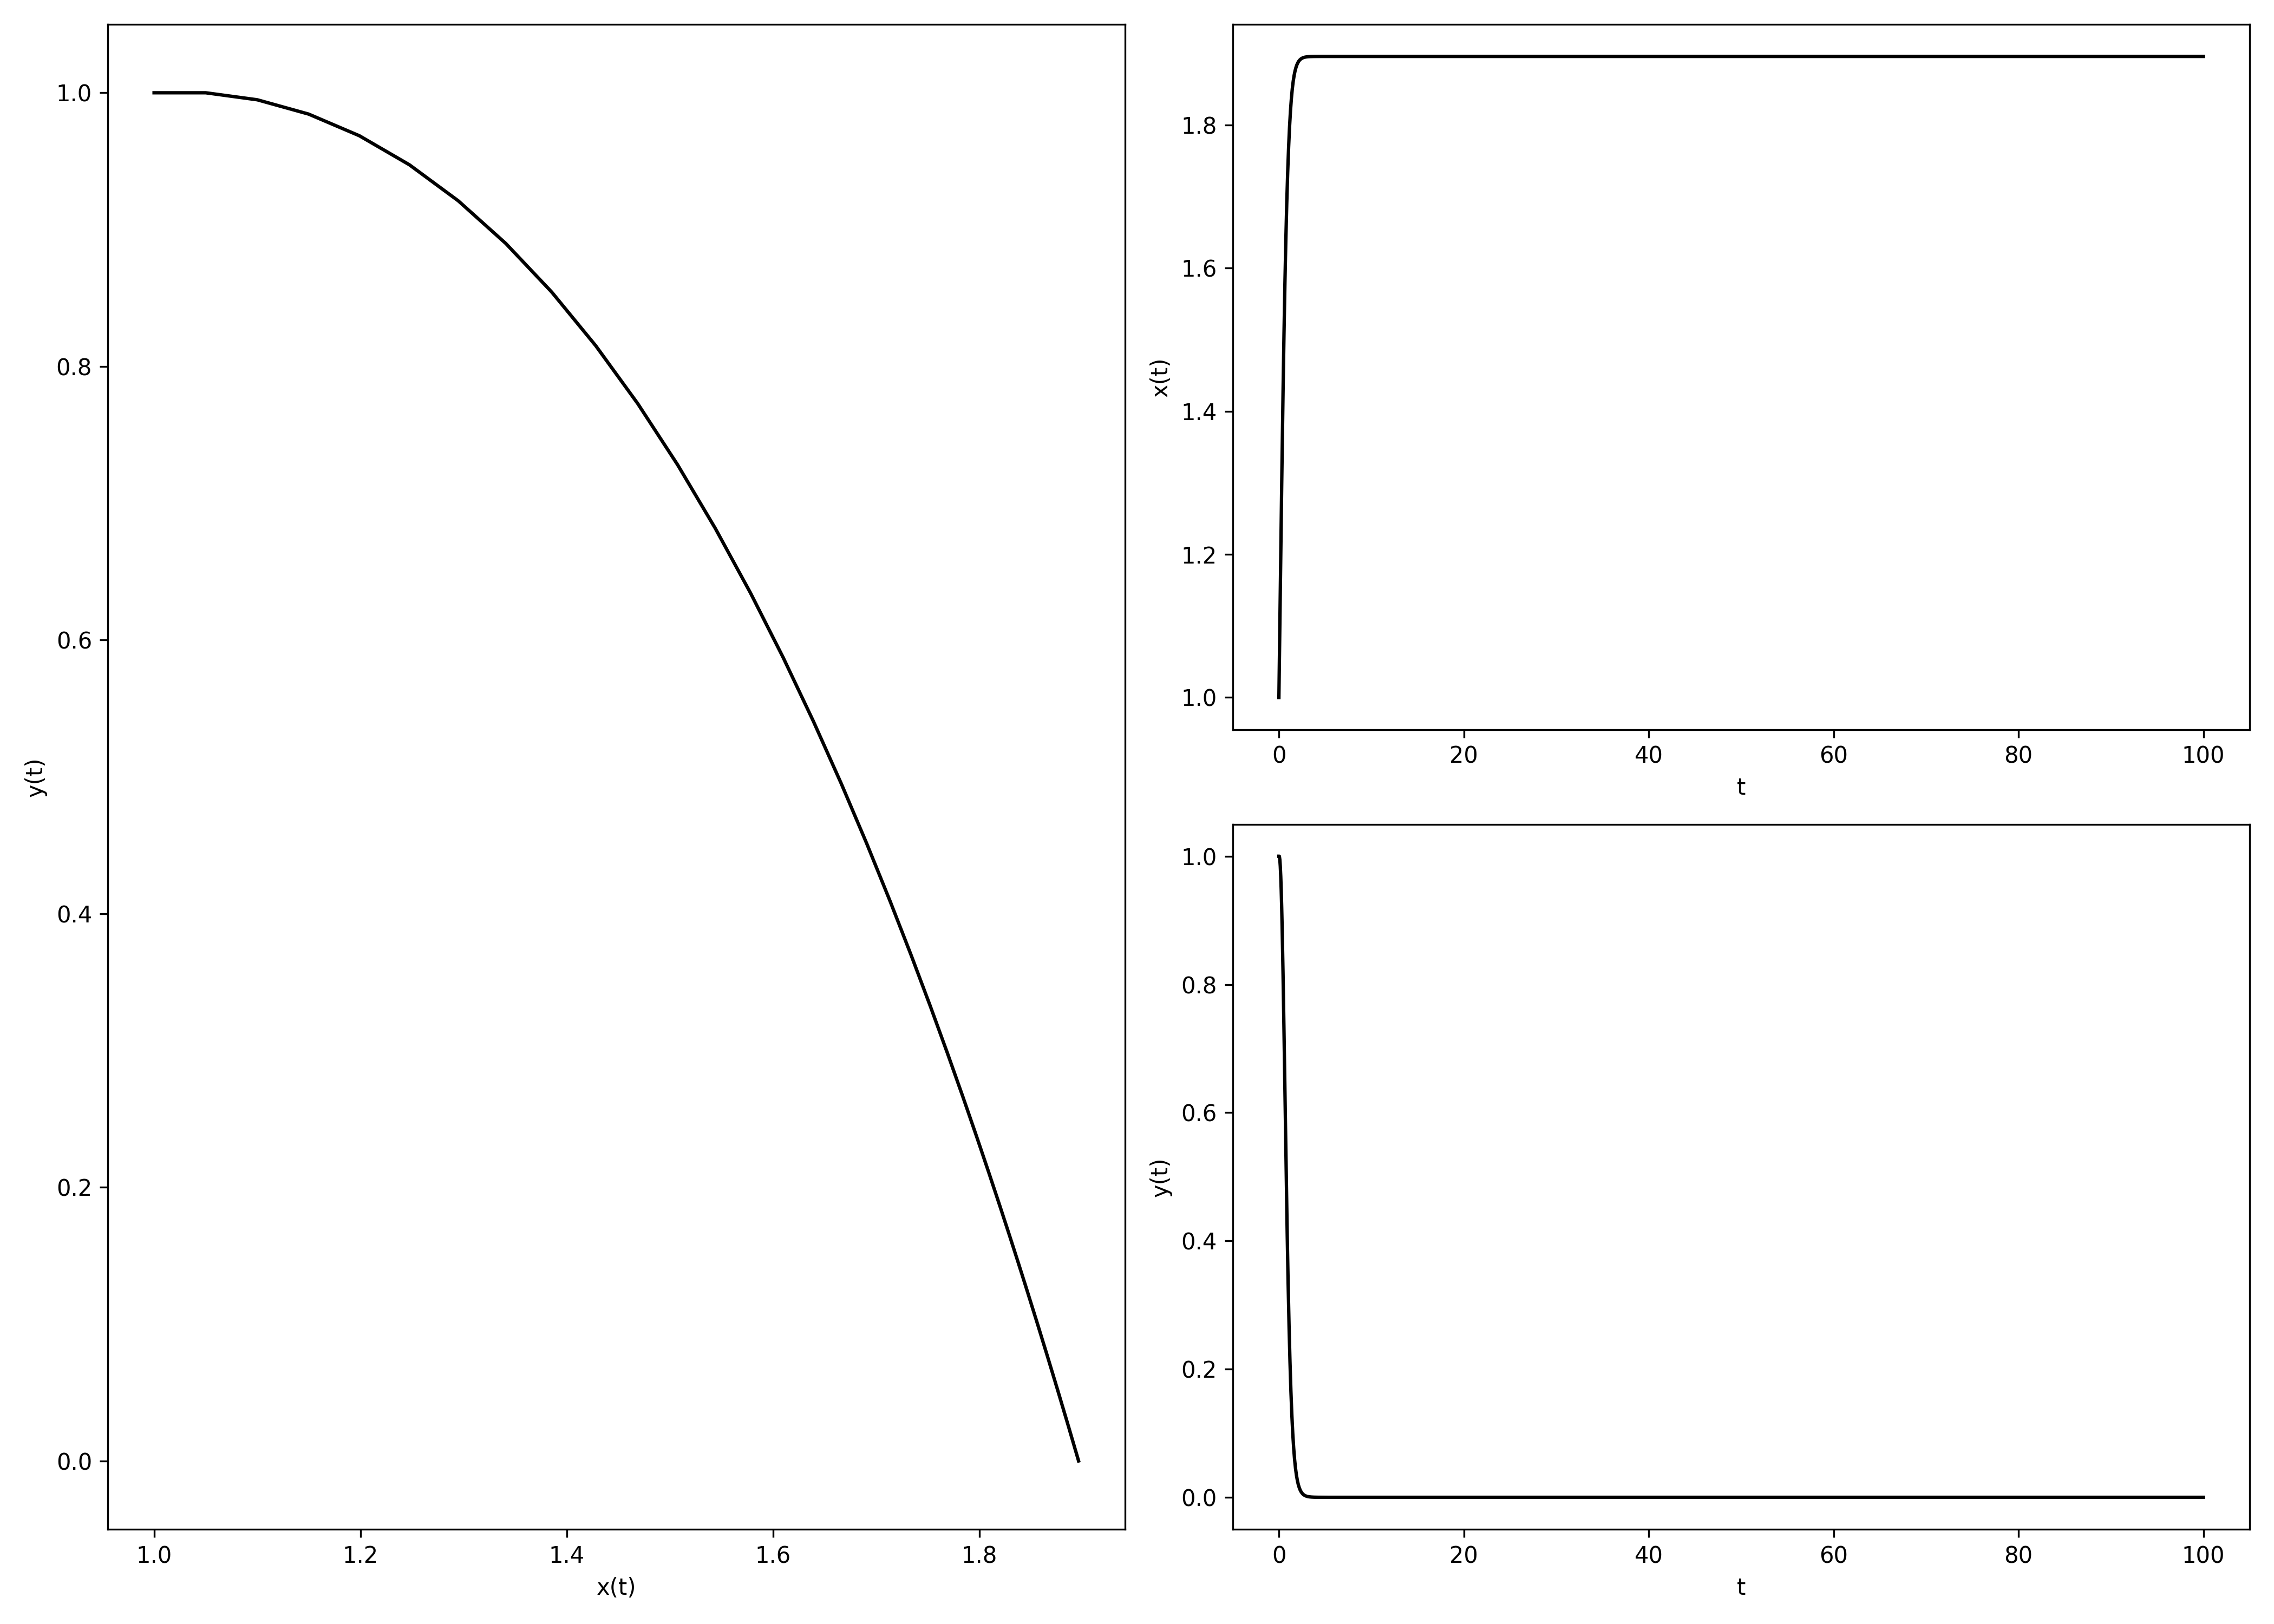
\includegraphics[scale=0.33]{x1,0y1,0mu1,0omega0,0t1,00e+02n2,00e+03.png}
\figcaption{$x_0=1,00, y_0=1.00, \mu=1.00, \omega=0.00, T = 200, N = 2000$}
% 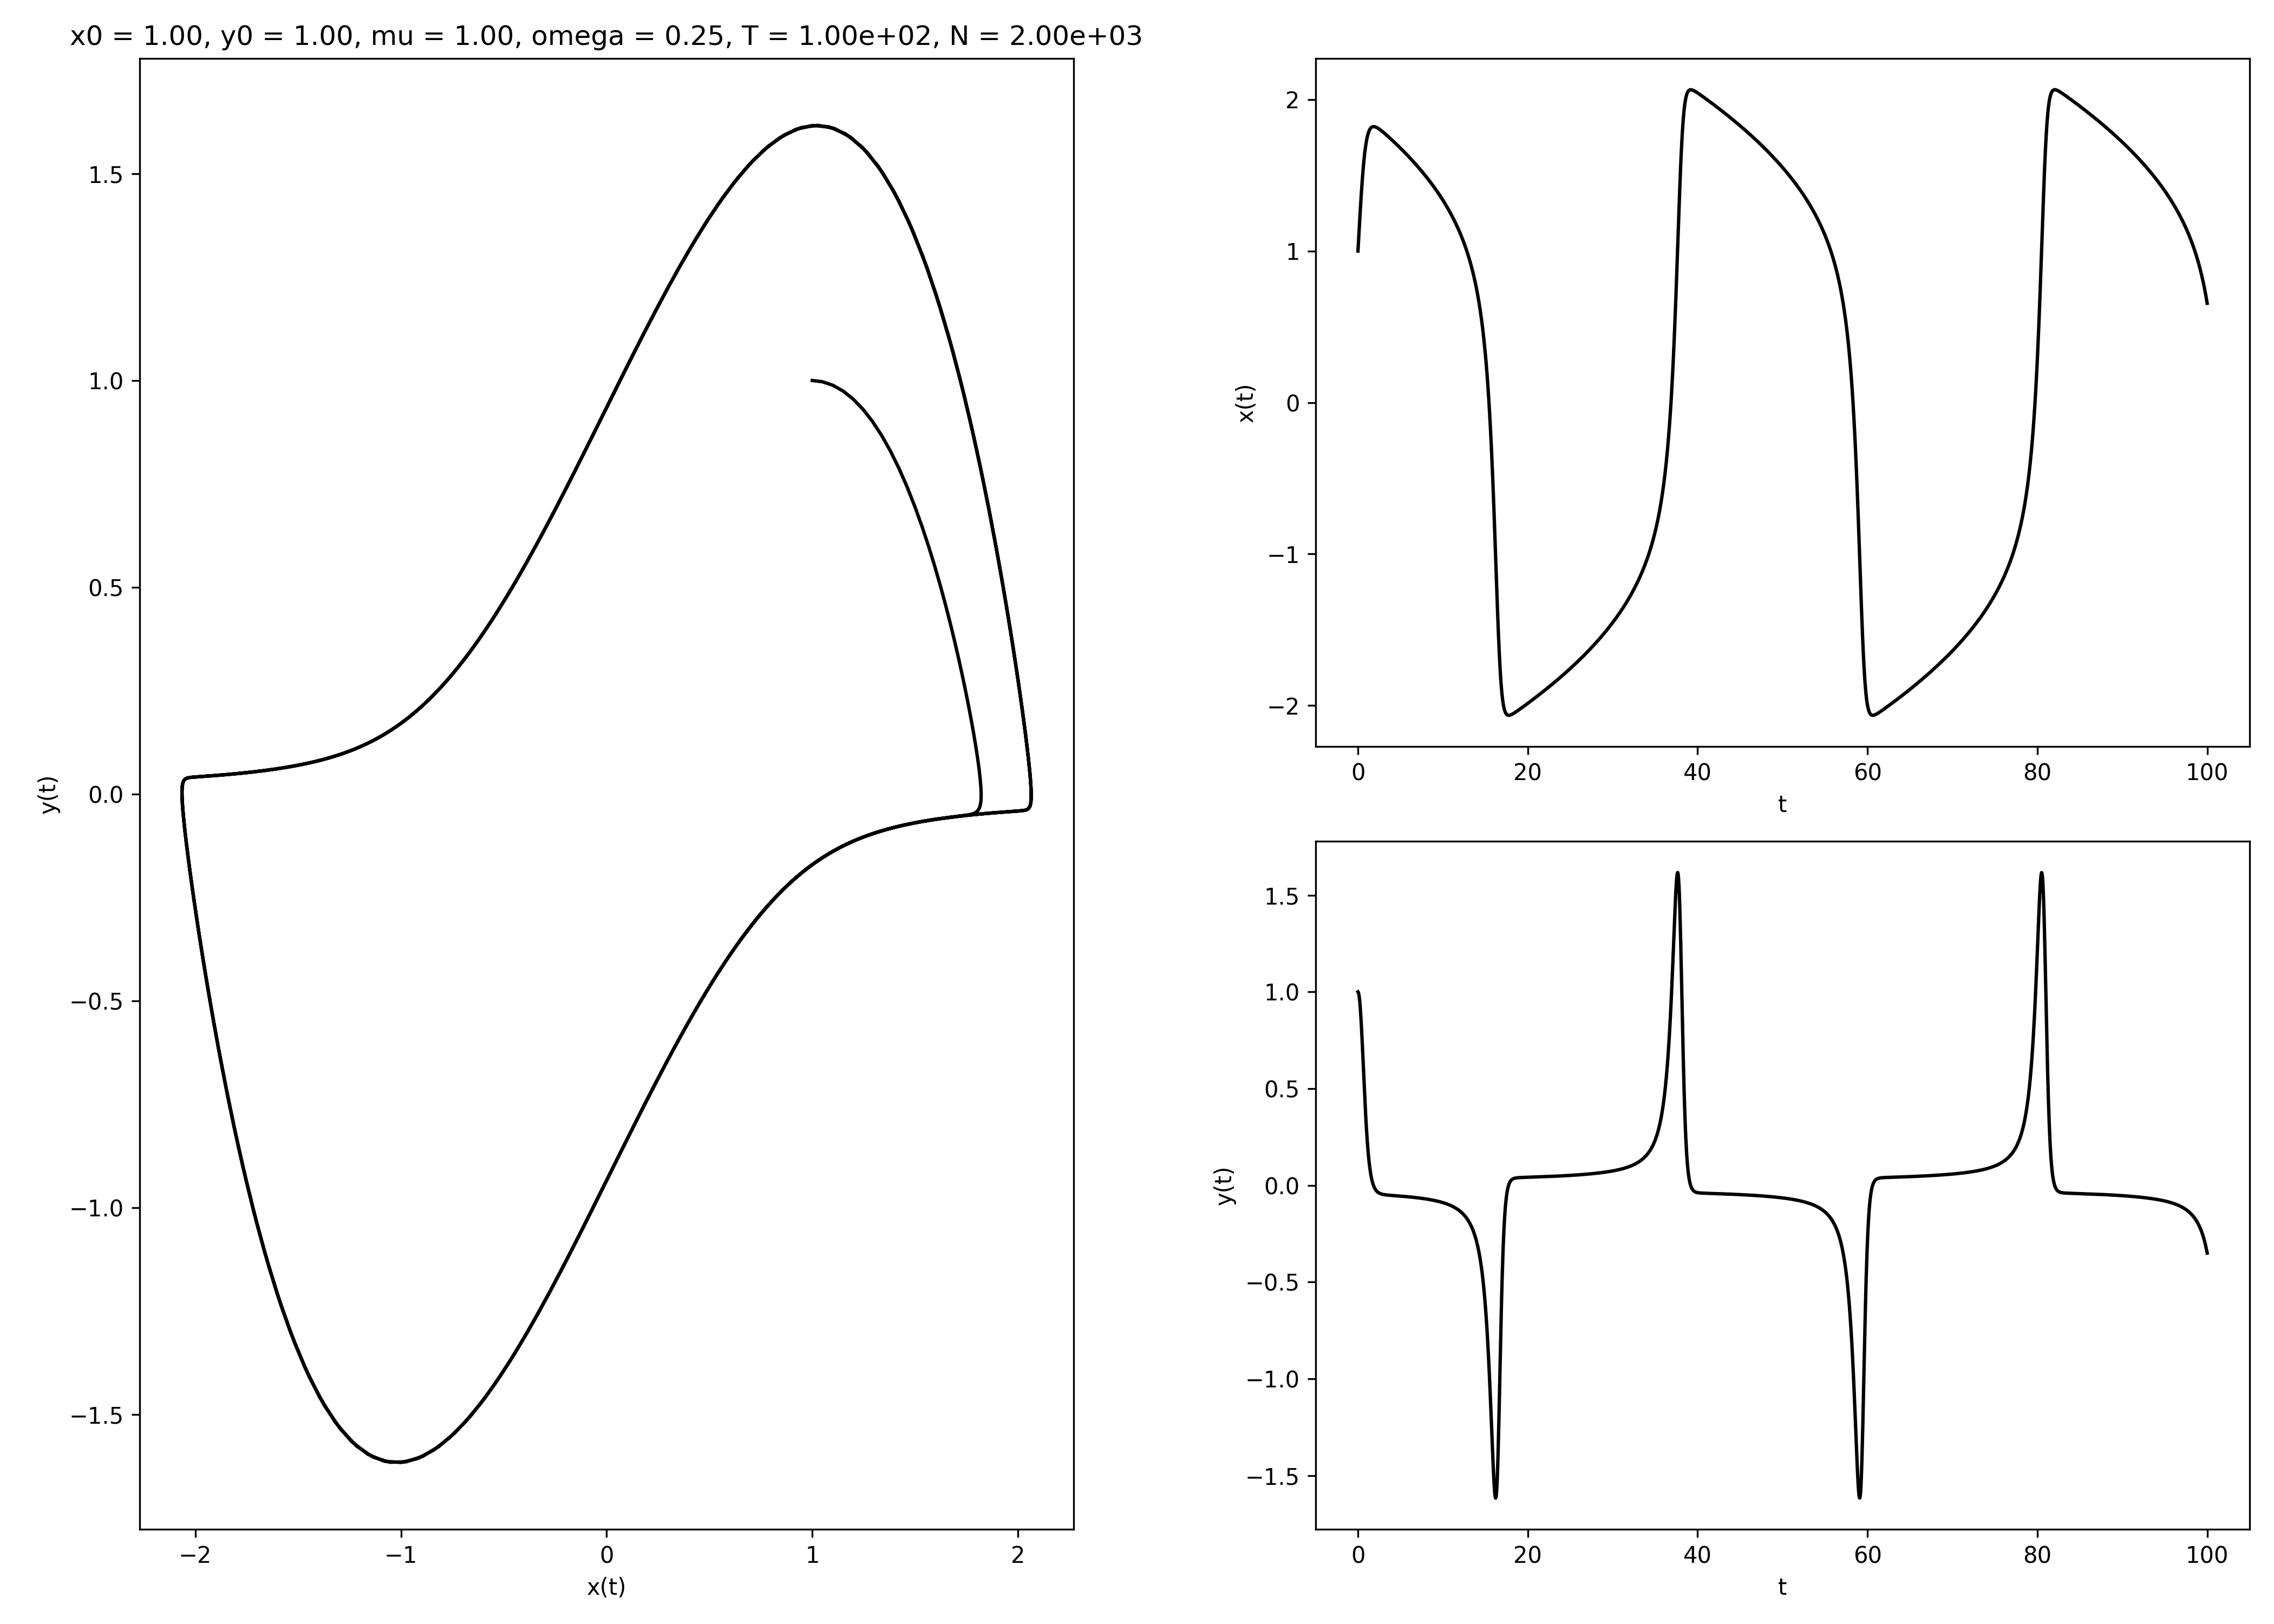
\includegraphics[scale=0.33]{x1,0y1,0mu1,0omega0,2t1,00e+02n2,00e+03.png}
% \figcaption{$x_0=1,00, y_0=1.00, \mu=1.00, \omega=0.25, T = 200, N = 2000$}
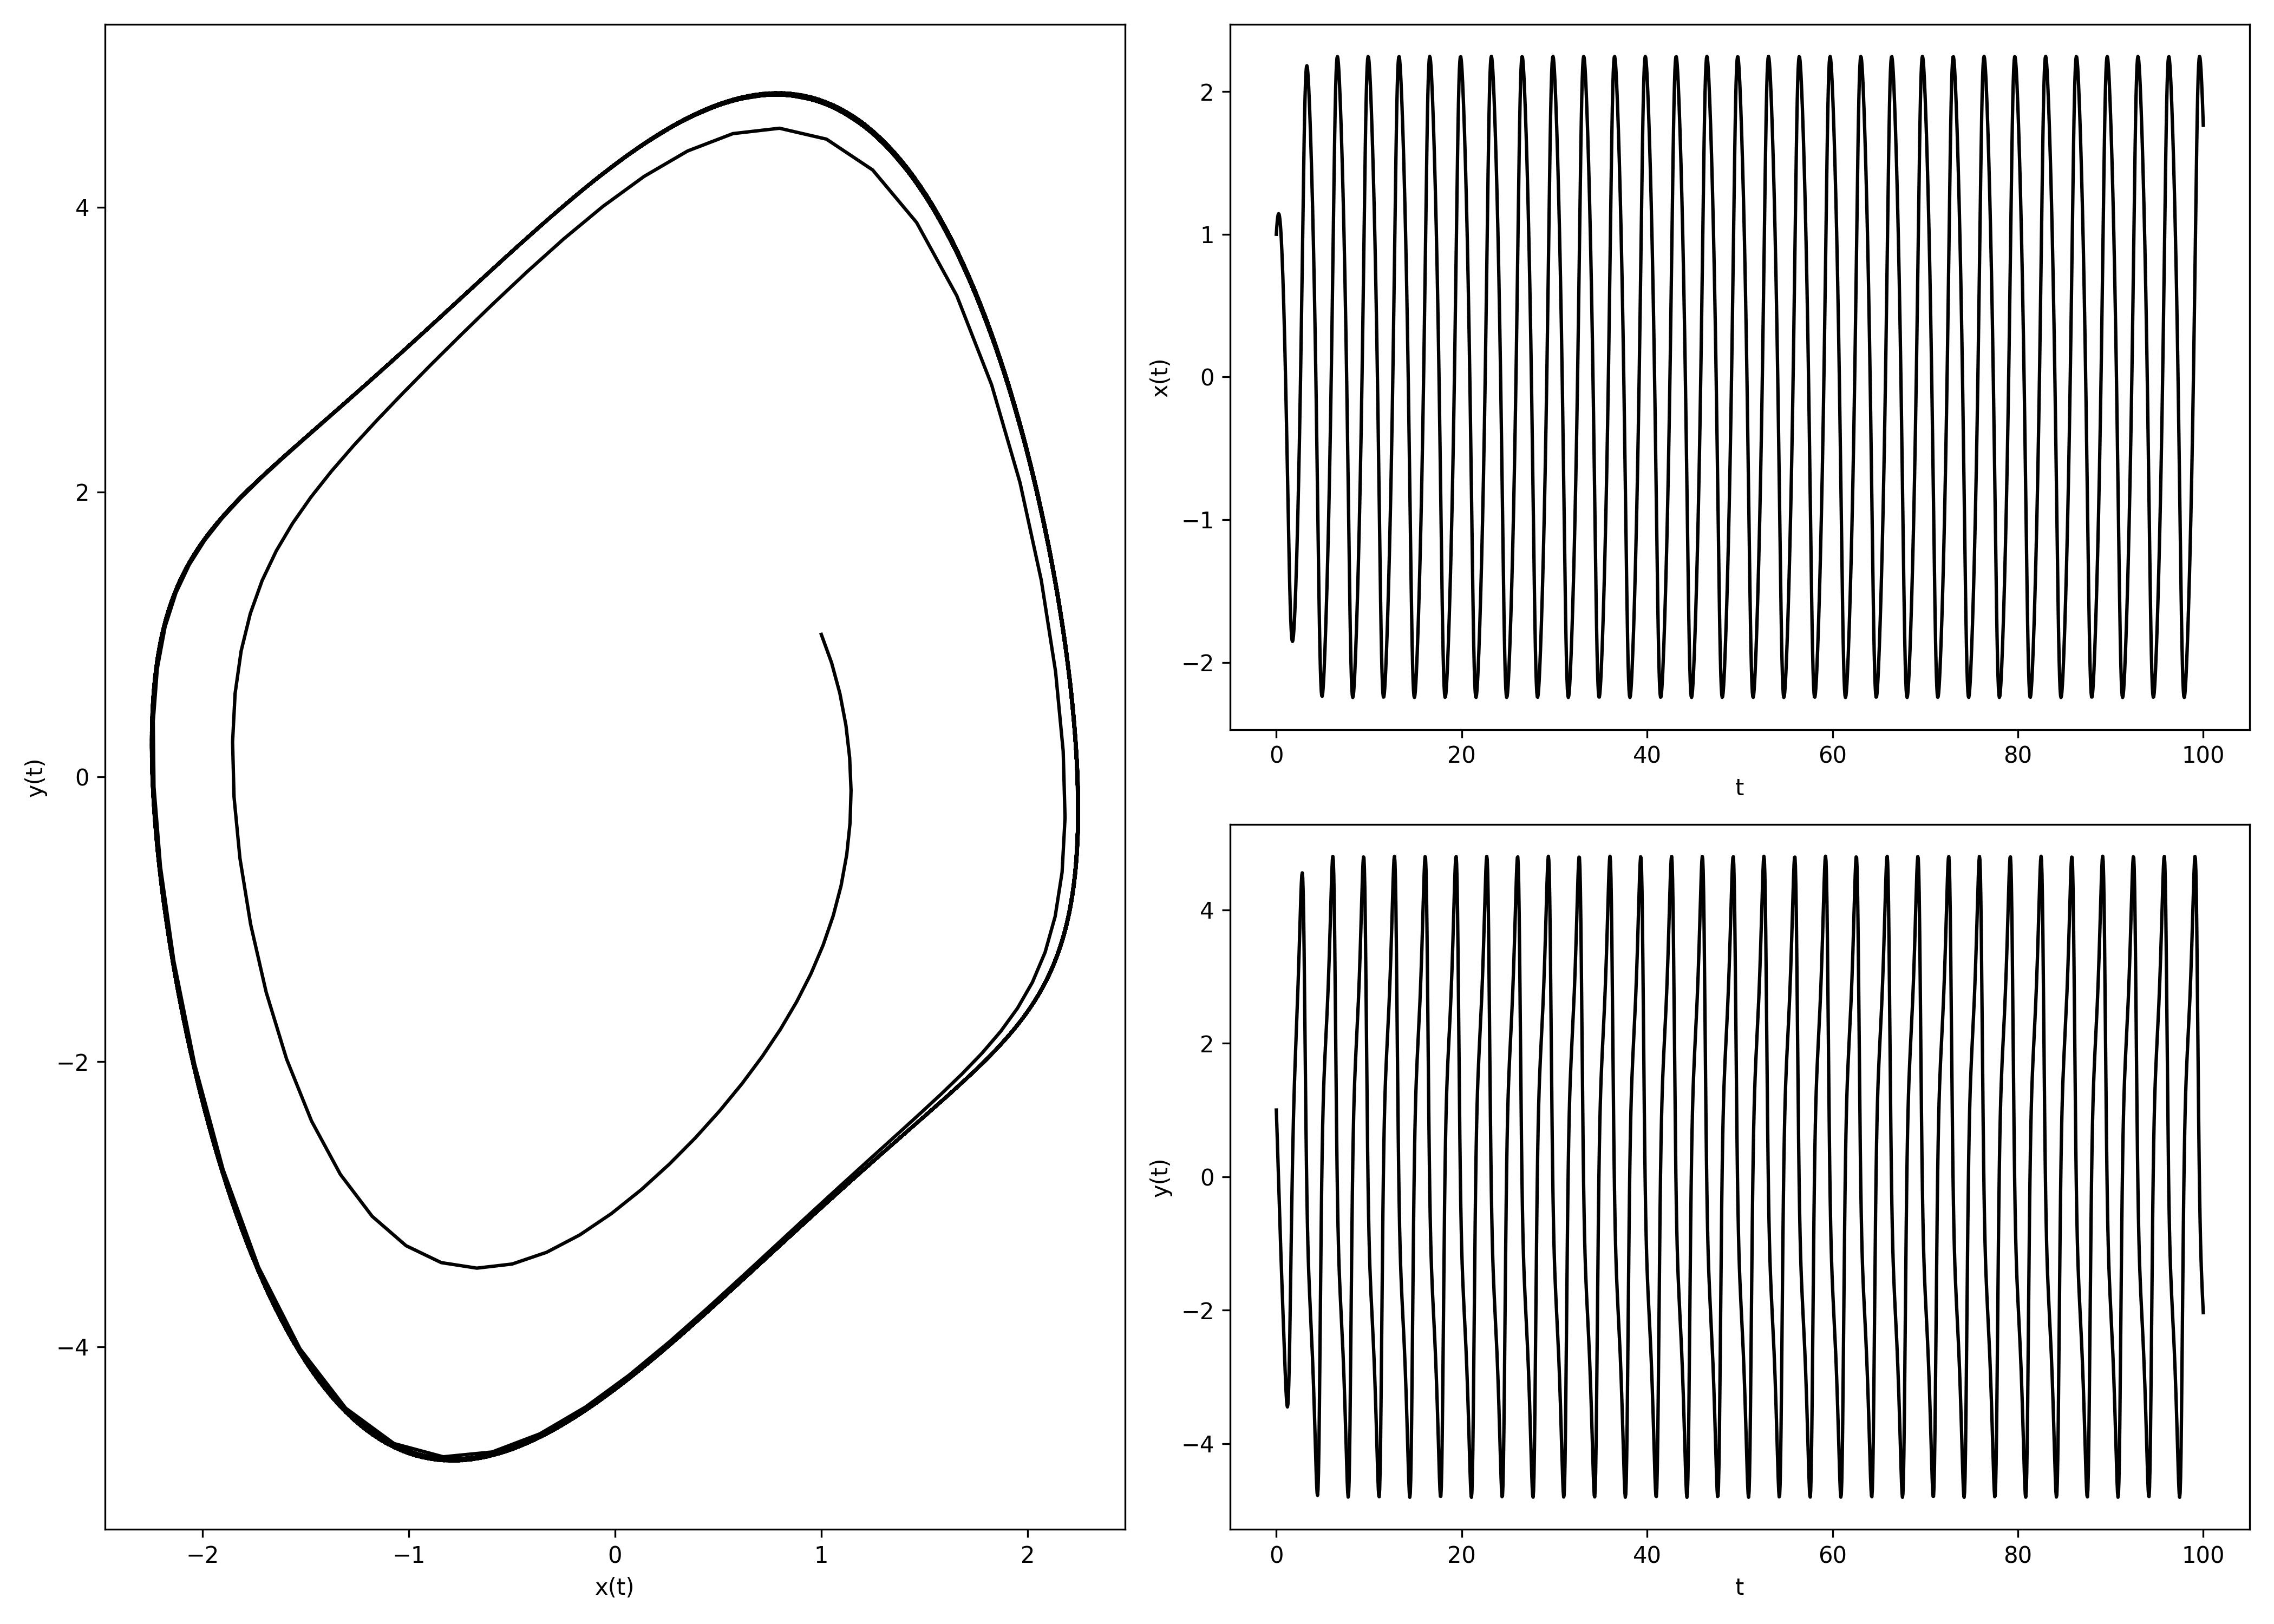
\includegraphics[scale=0.33]{x1,0y1,0mu1,0omega2,0t1,00e+02n2,00e+03.png}
\figcaption{$x_0=1,00, y_0=1.00, \mu=1.00, \omega=2.00, T = 200, N = 2000$}
%パラメーター初期値
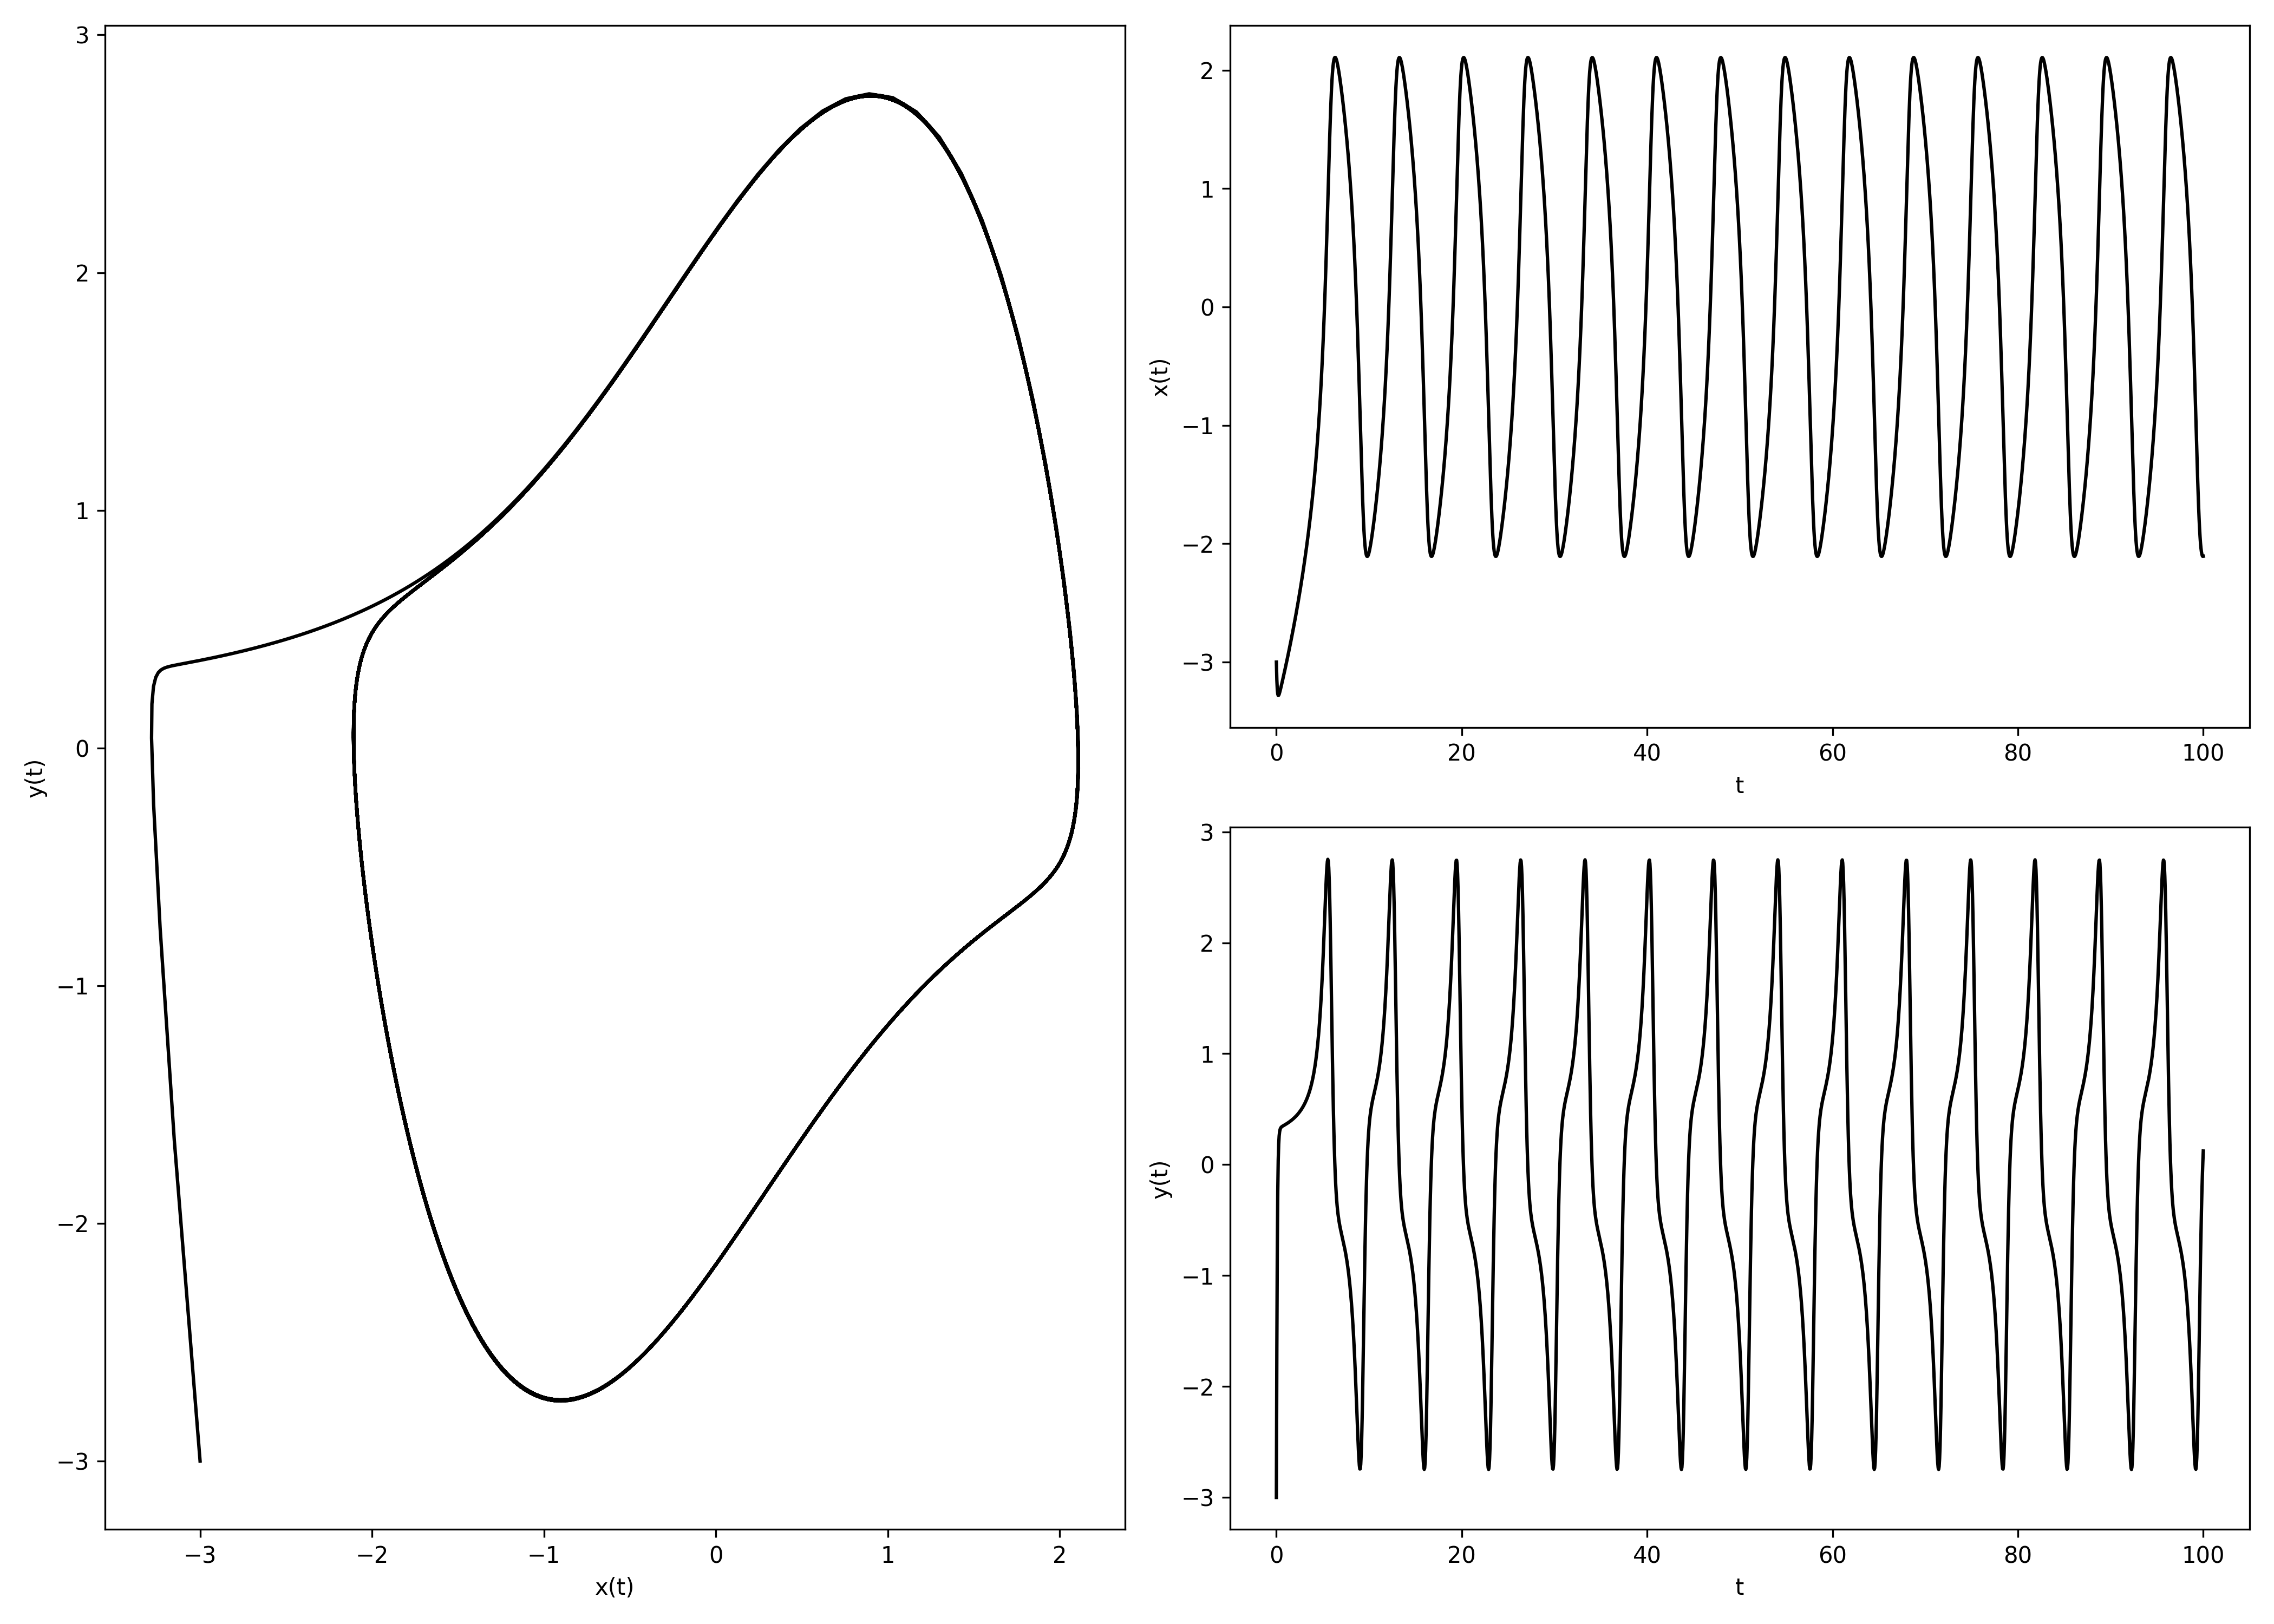
\includegraphics[scale=0.33]{x-3,0y-3,0mu1,0omega1,0t1,00e+02n2,00e+03.png}
\figcaption{$x_0=-3.00, y_0=-3.00, \mu=1,00, \omega=1.00, T = 200, N = 2000$}
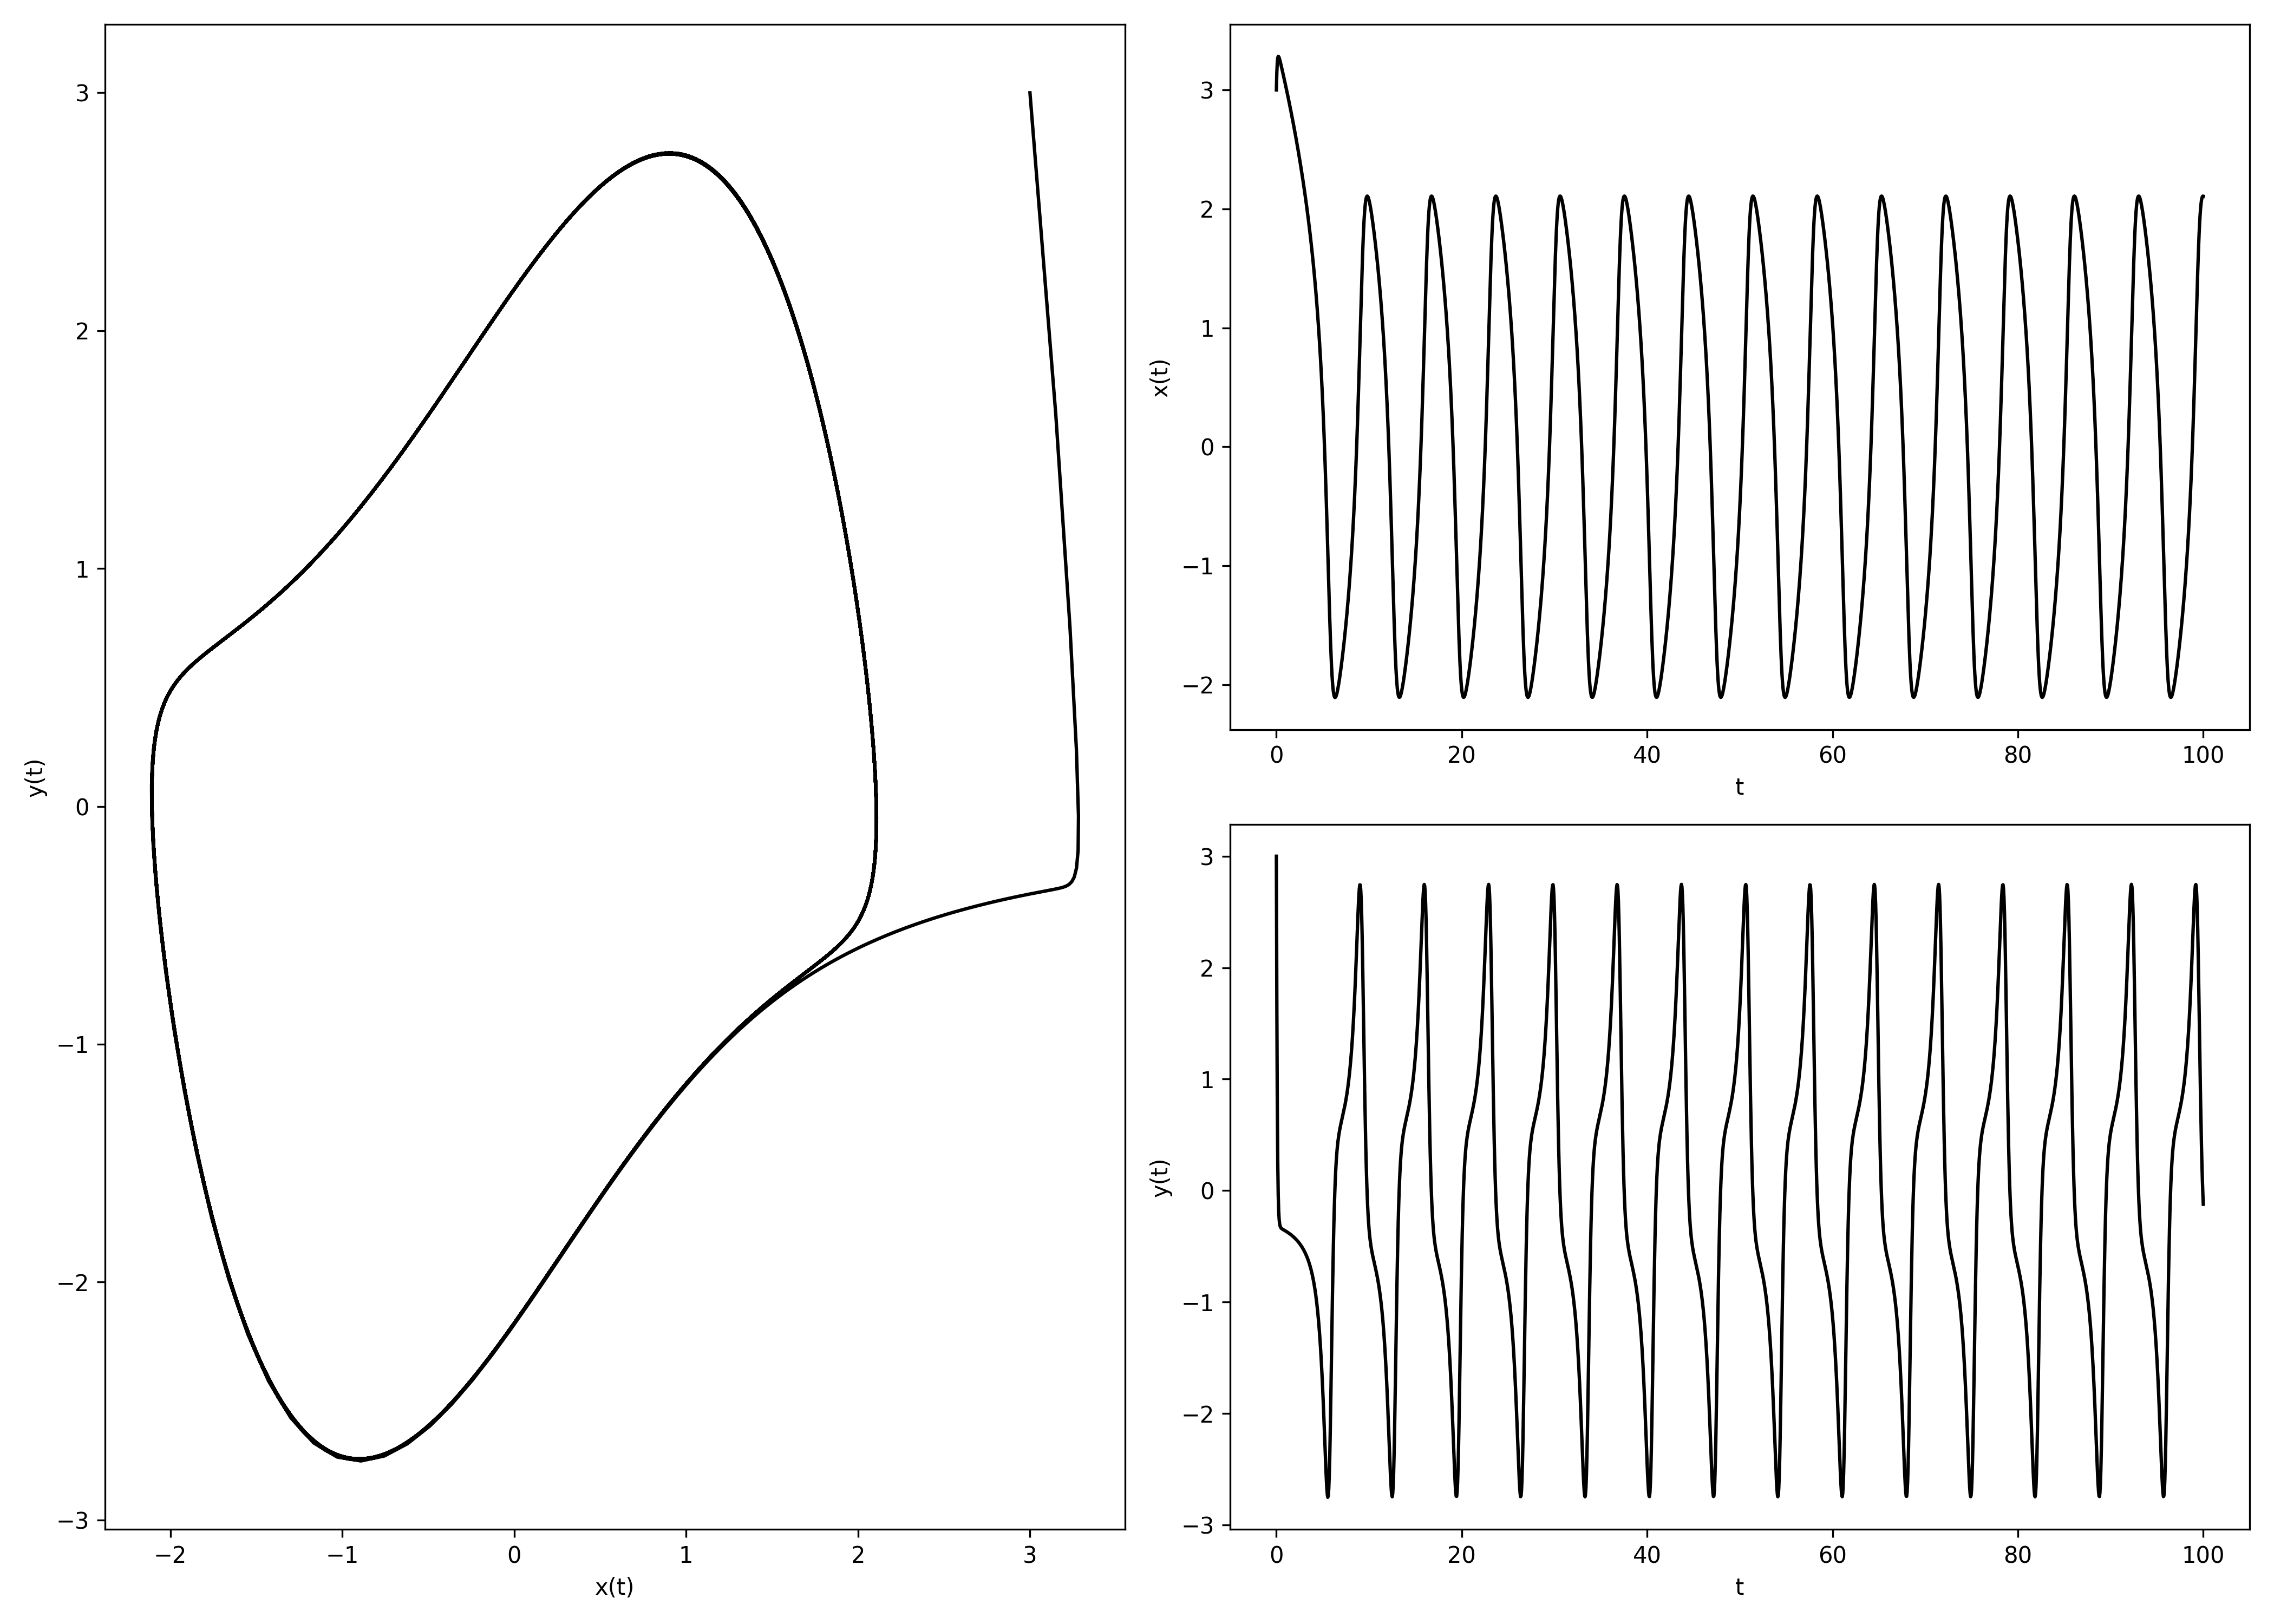
\includegraphics[scale=0.33]{x3,0y3,0mu1,0omega1,0t1,00e+02n2,00e+03.png}
\figcaption{$x_0=3.00, y_0=3.00, \mu=1,00, \omega=1.00, T = 200, N = 2000$}
%N = 10000
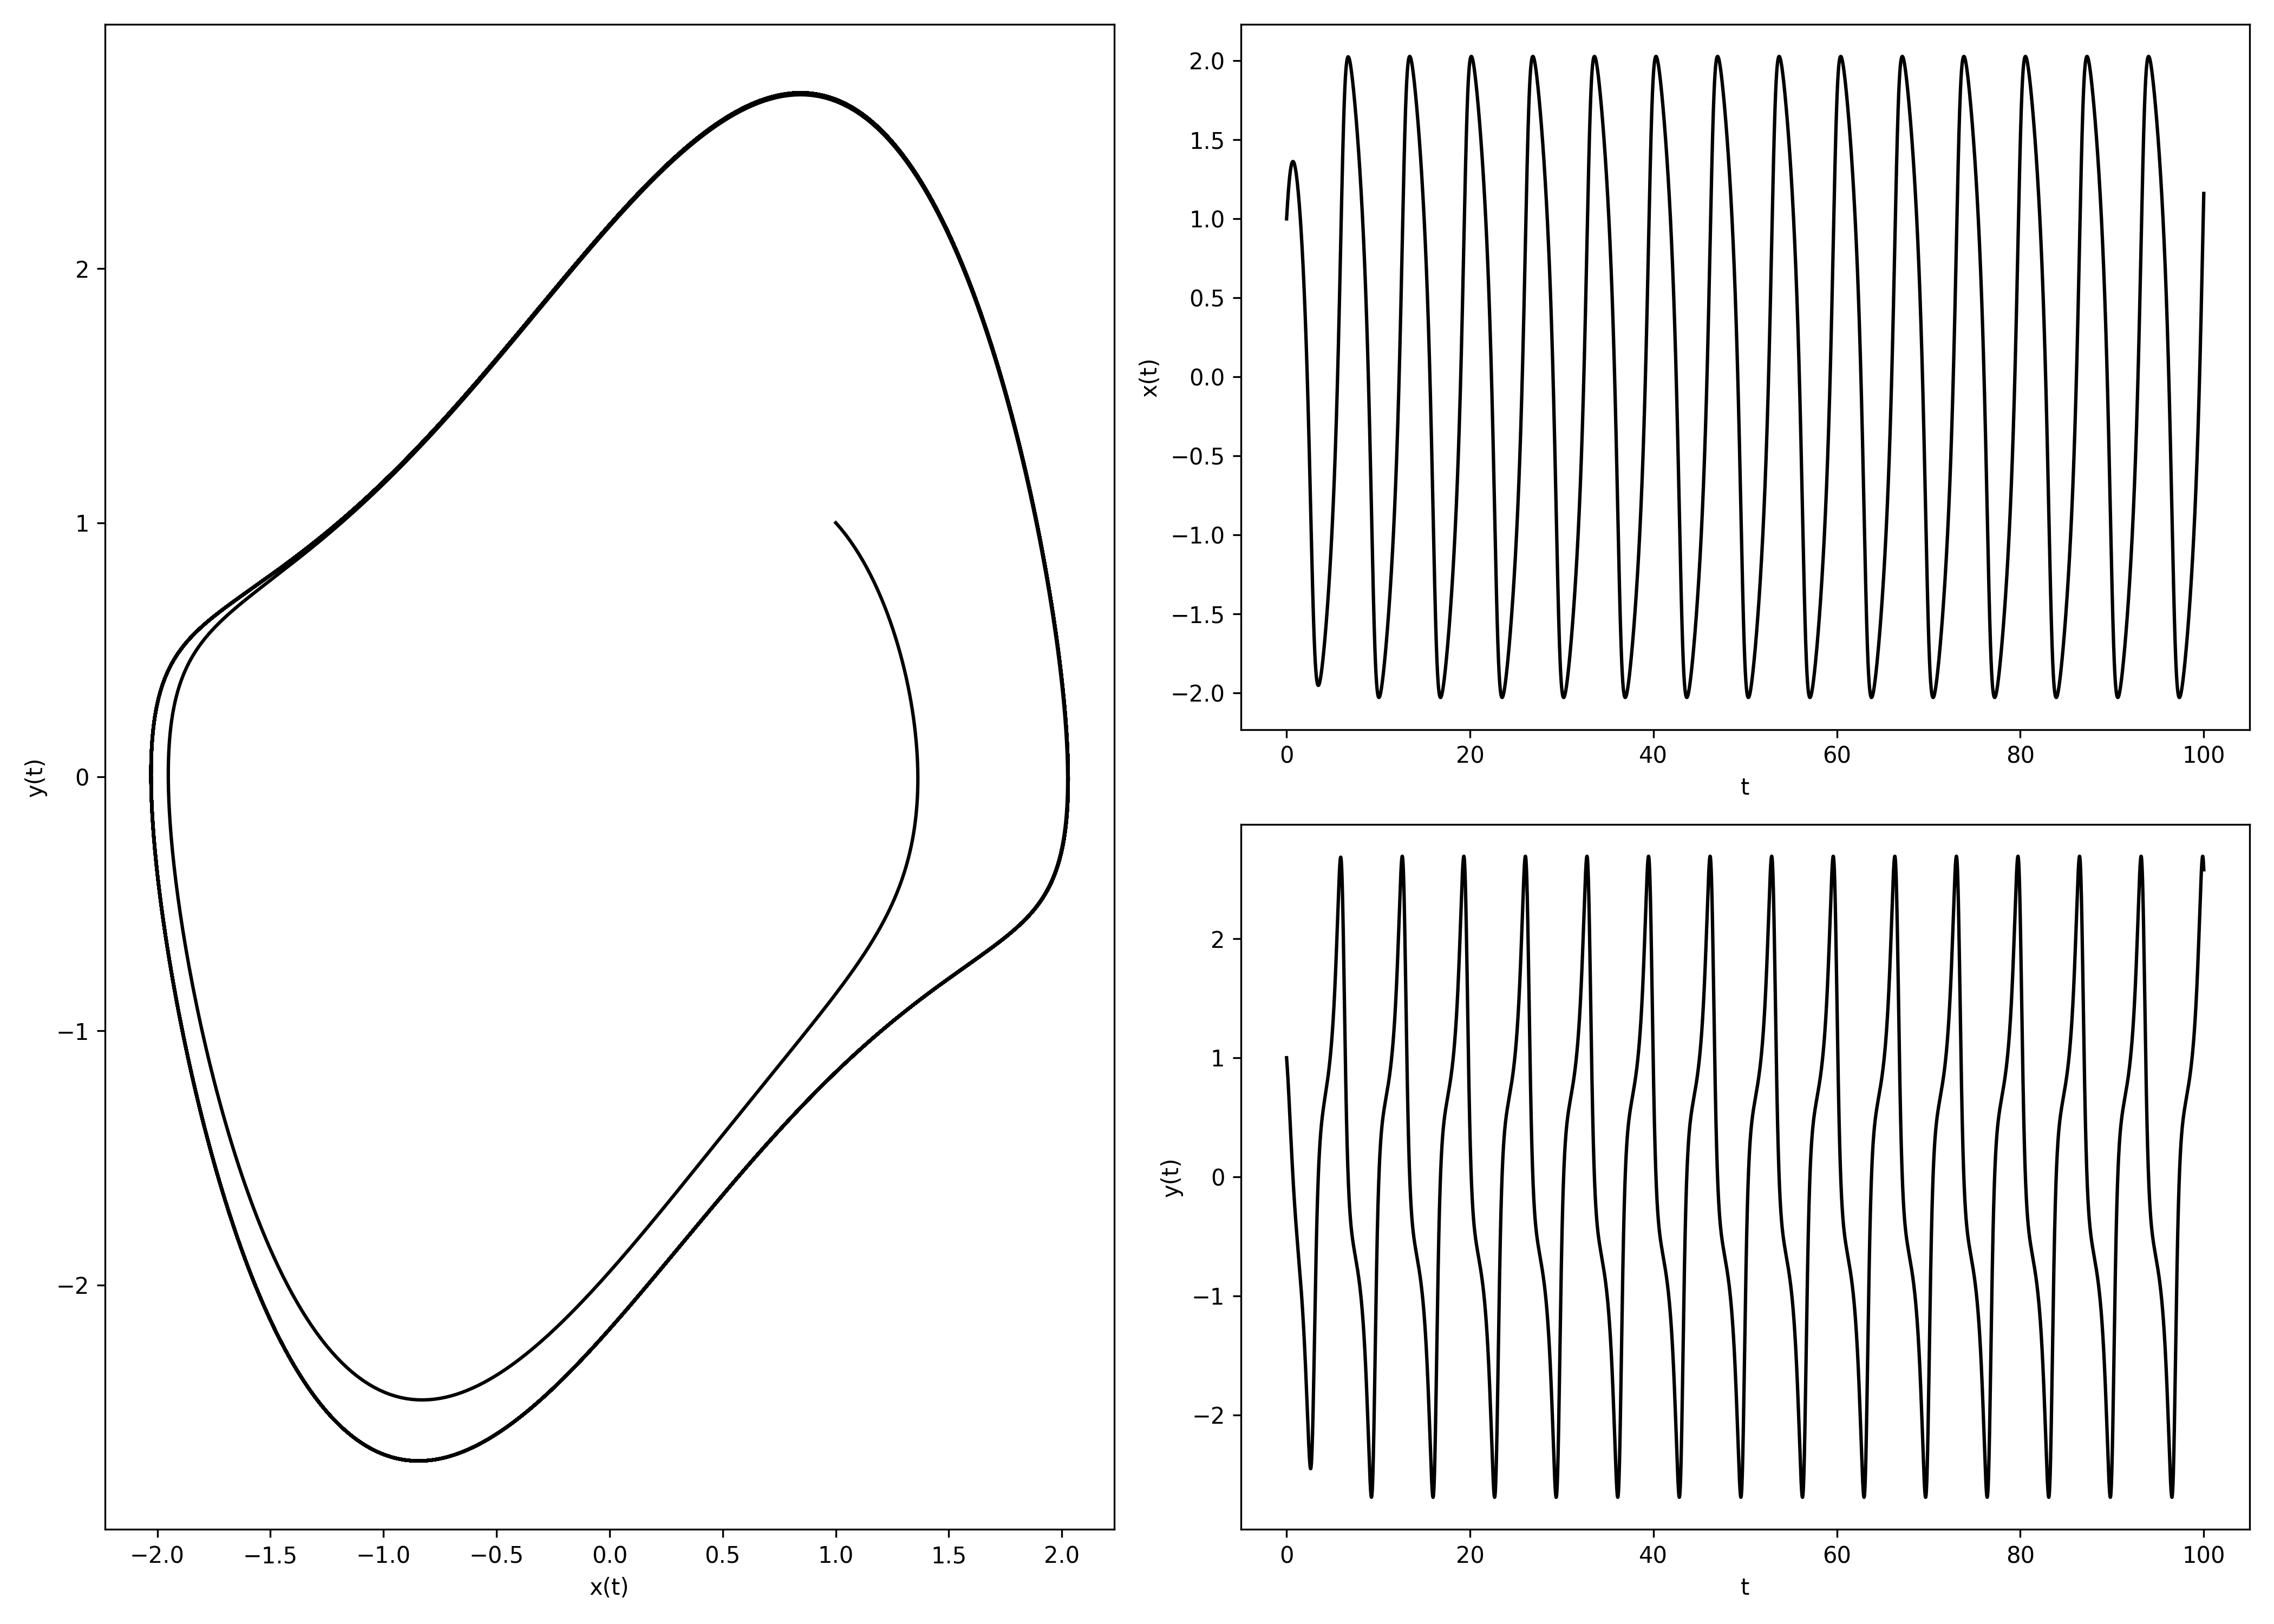
\includegraphics[scale=0.33]{x1,0y1,0mu1,0omega1,0t1,00e+02n1,00e+04.png}
\figcaption{$x_0=1,00, y_0=1.00, \mu=1.00, \omega=1.00, T = 100, N = 10000$}
%パラメーターmu
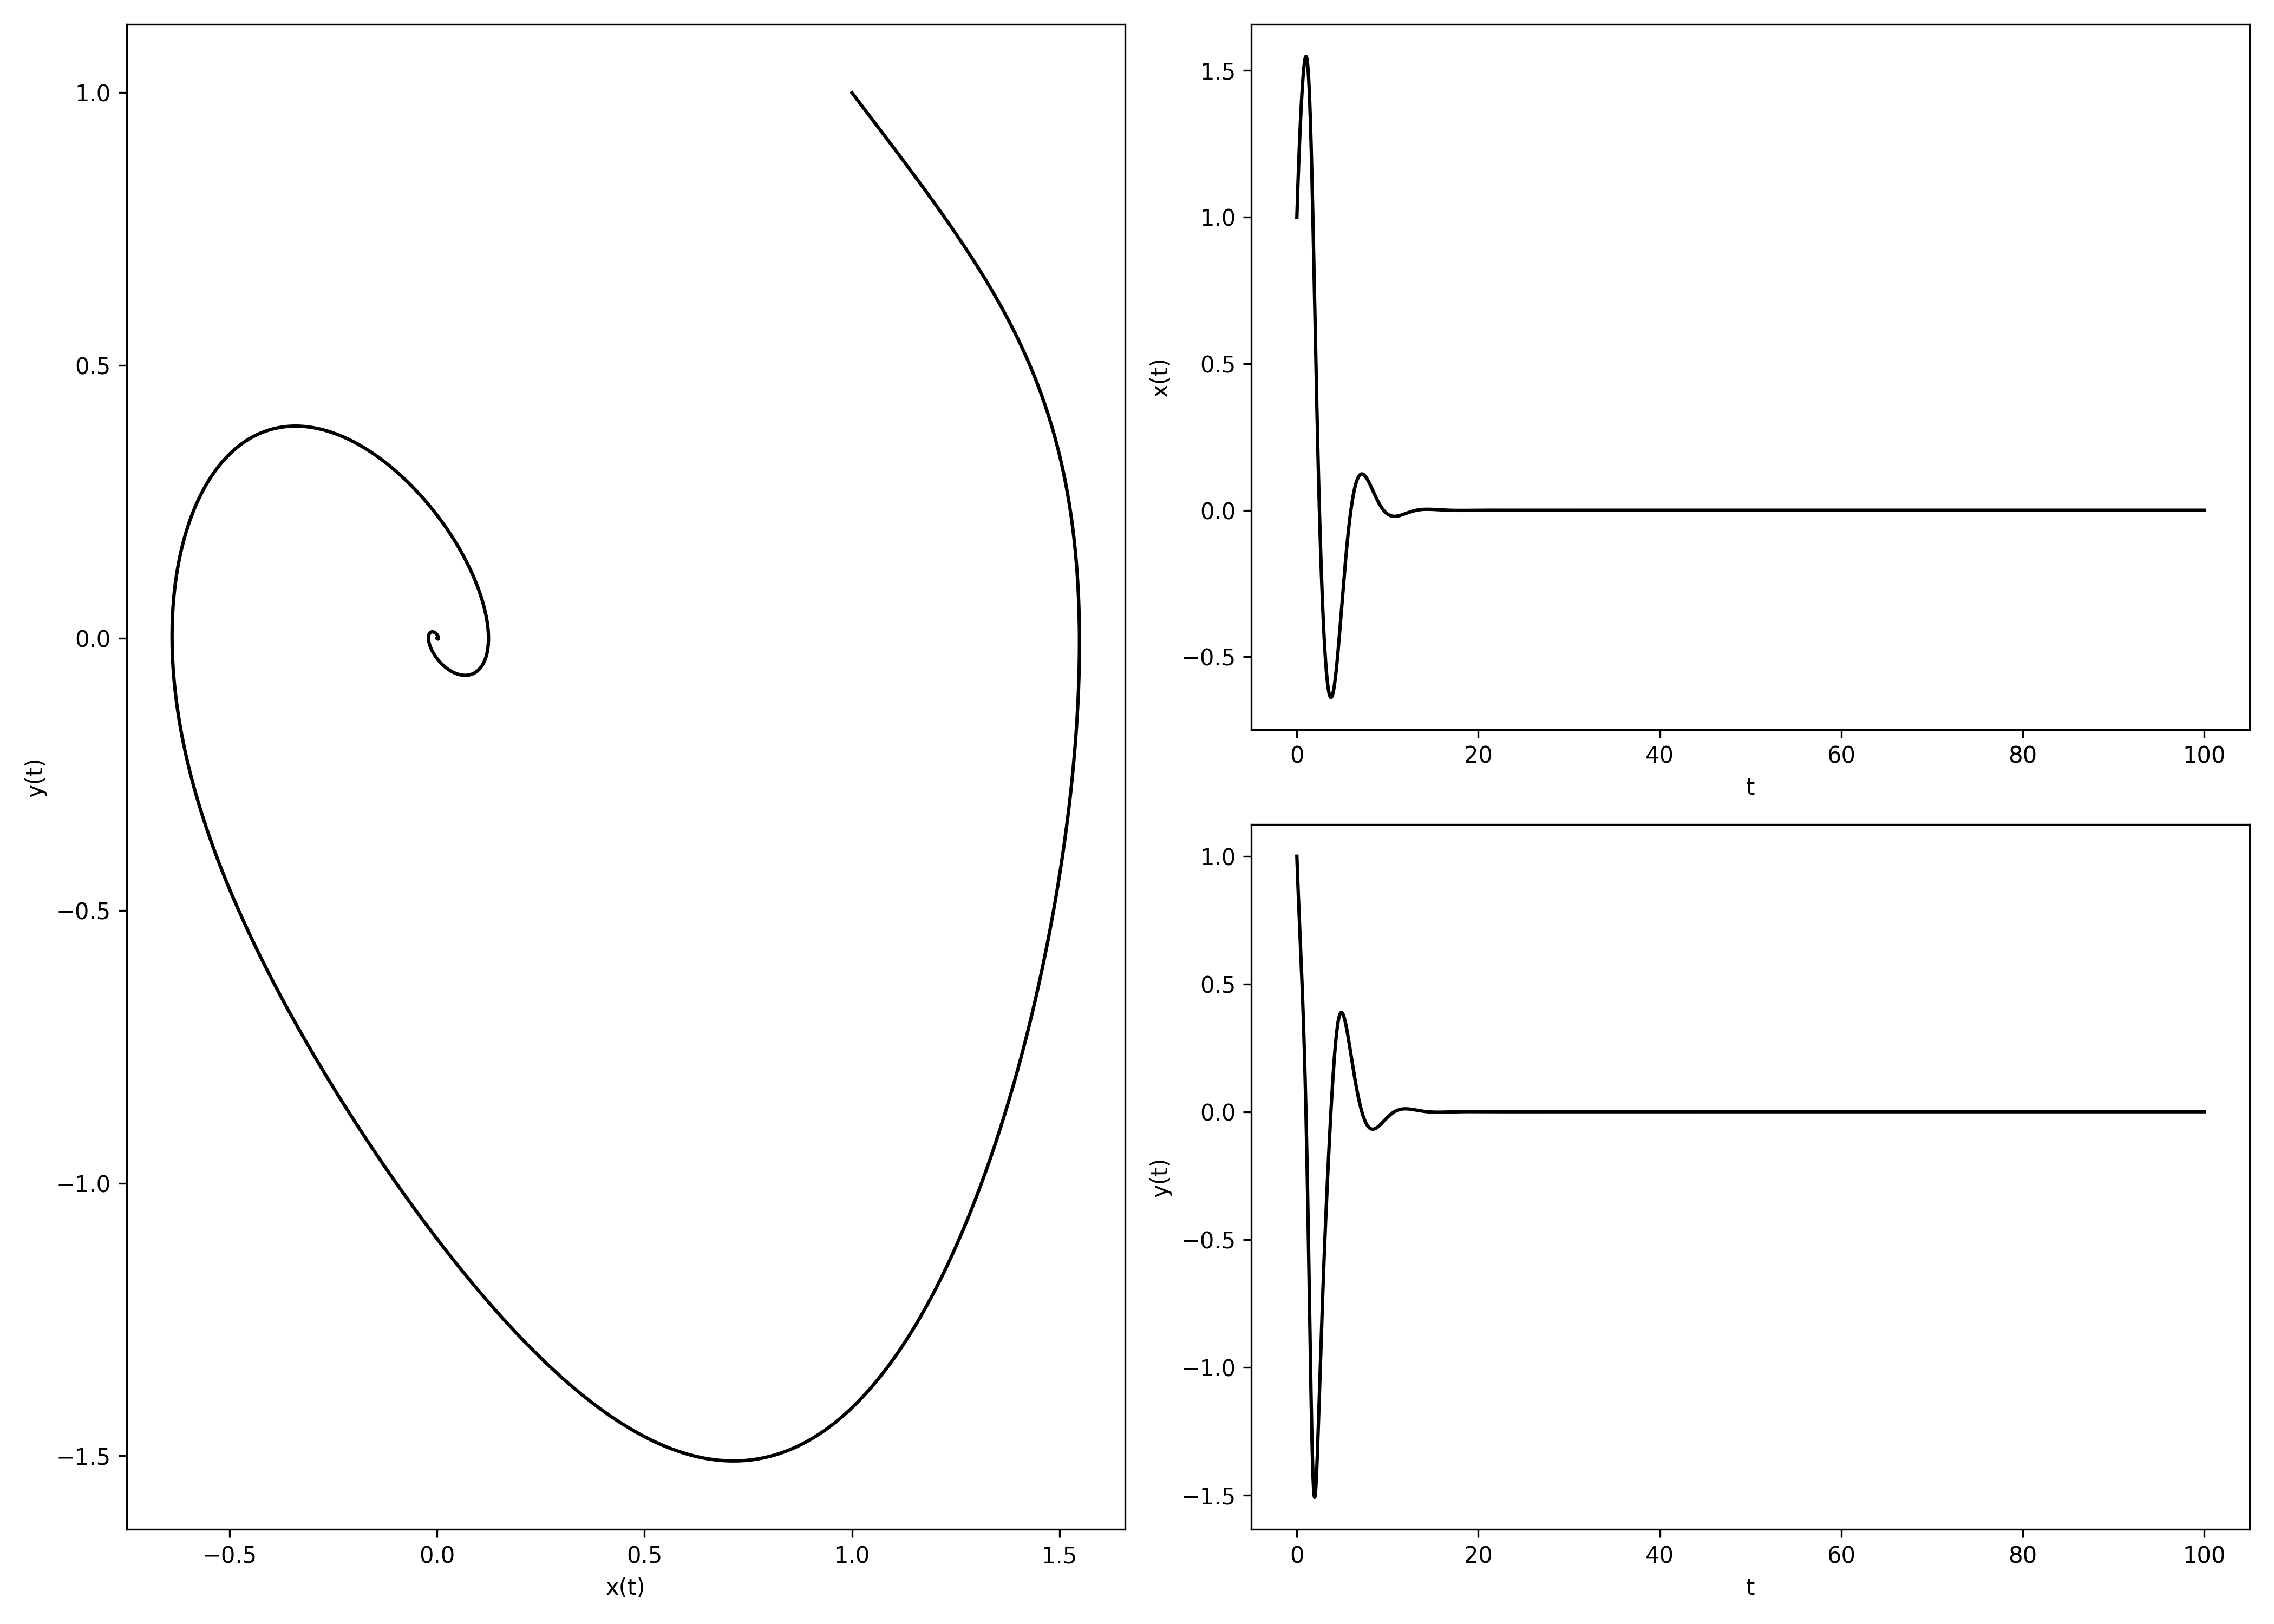
\includegraphics[scale=0.33]{x1,0y1,0mu-1,0omega1,0t1,00e+02n1,00e+04.png}
\figcaption{$x_0=1,00, y_0=1.00, \mu=-1.00, \omega=1.00, T = 100, N = 10000$}
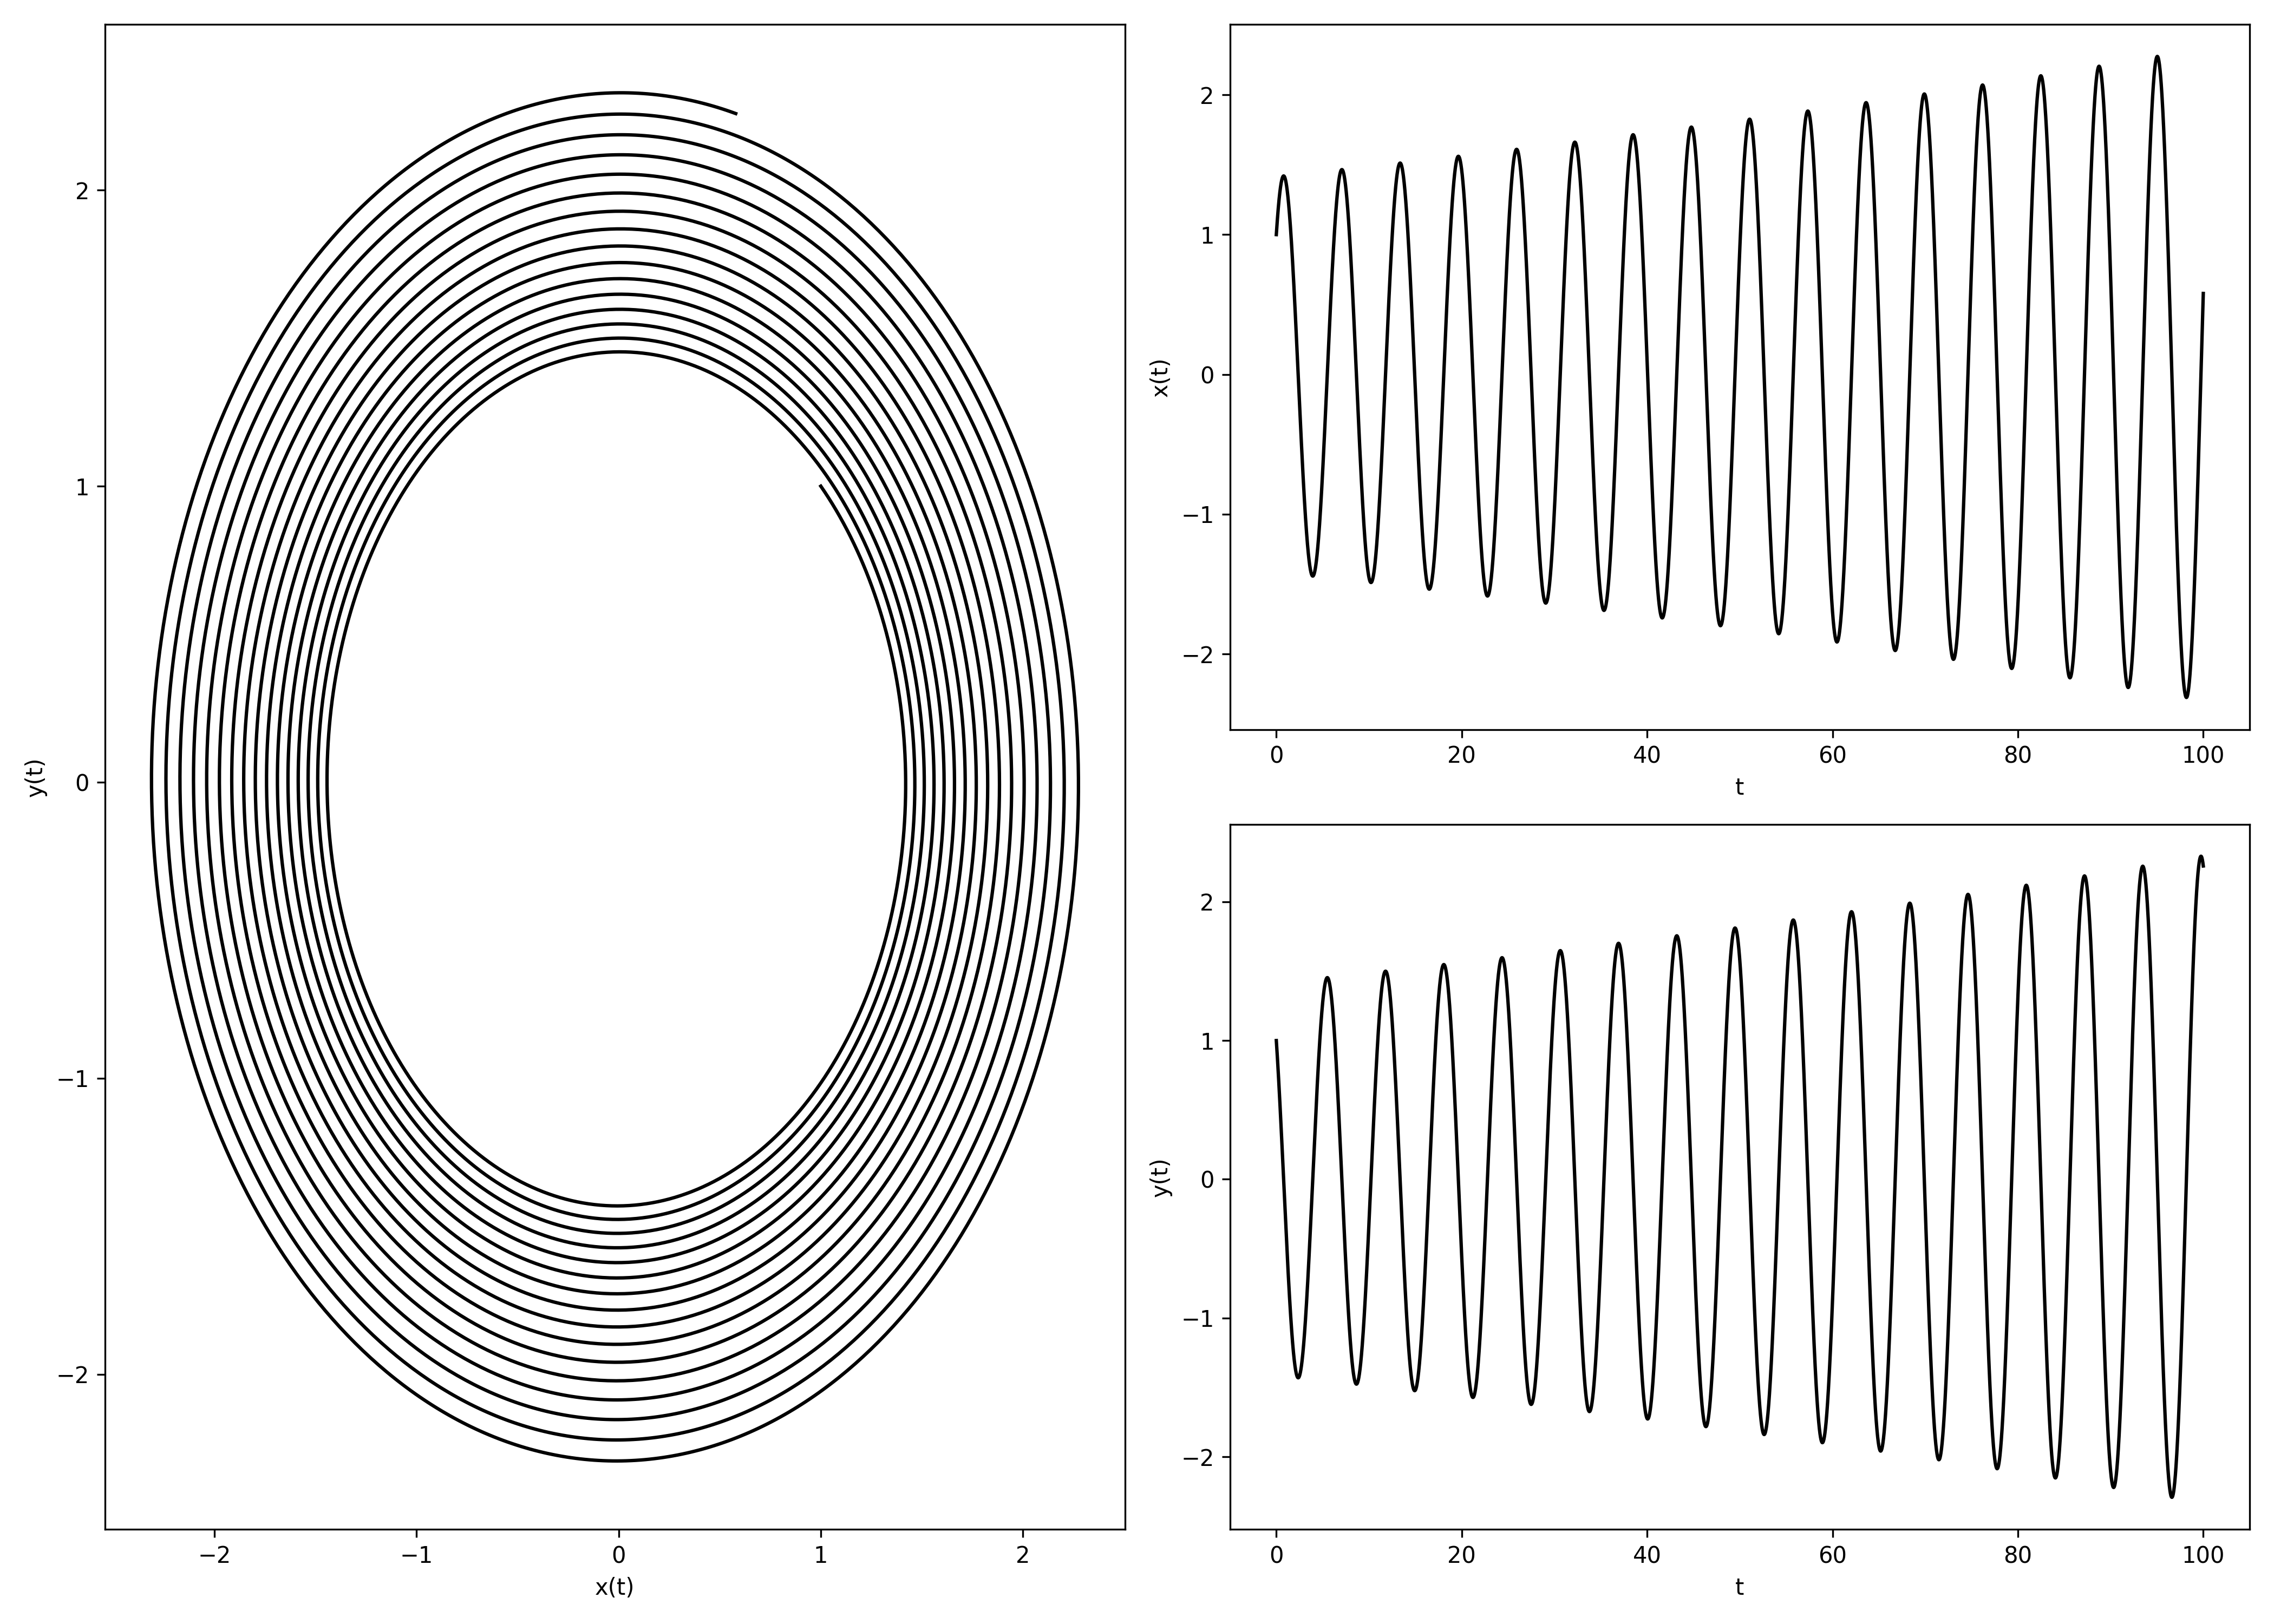
\includegraphics[scale=0.33]{x1,0y1,0mu0,0omega1,0t1,00e+02n1,00e+04.png}
\figcaption{$x_0=1,00, y_0=1.00, \mu=0.00, \omega=1.00, T = 100, N = 10000$}
% 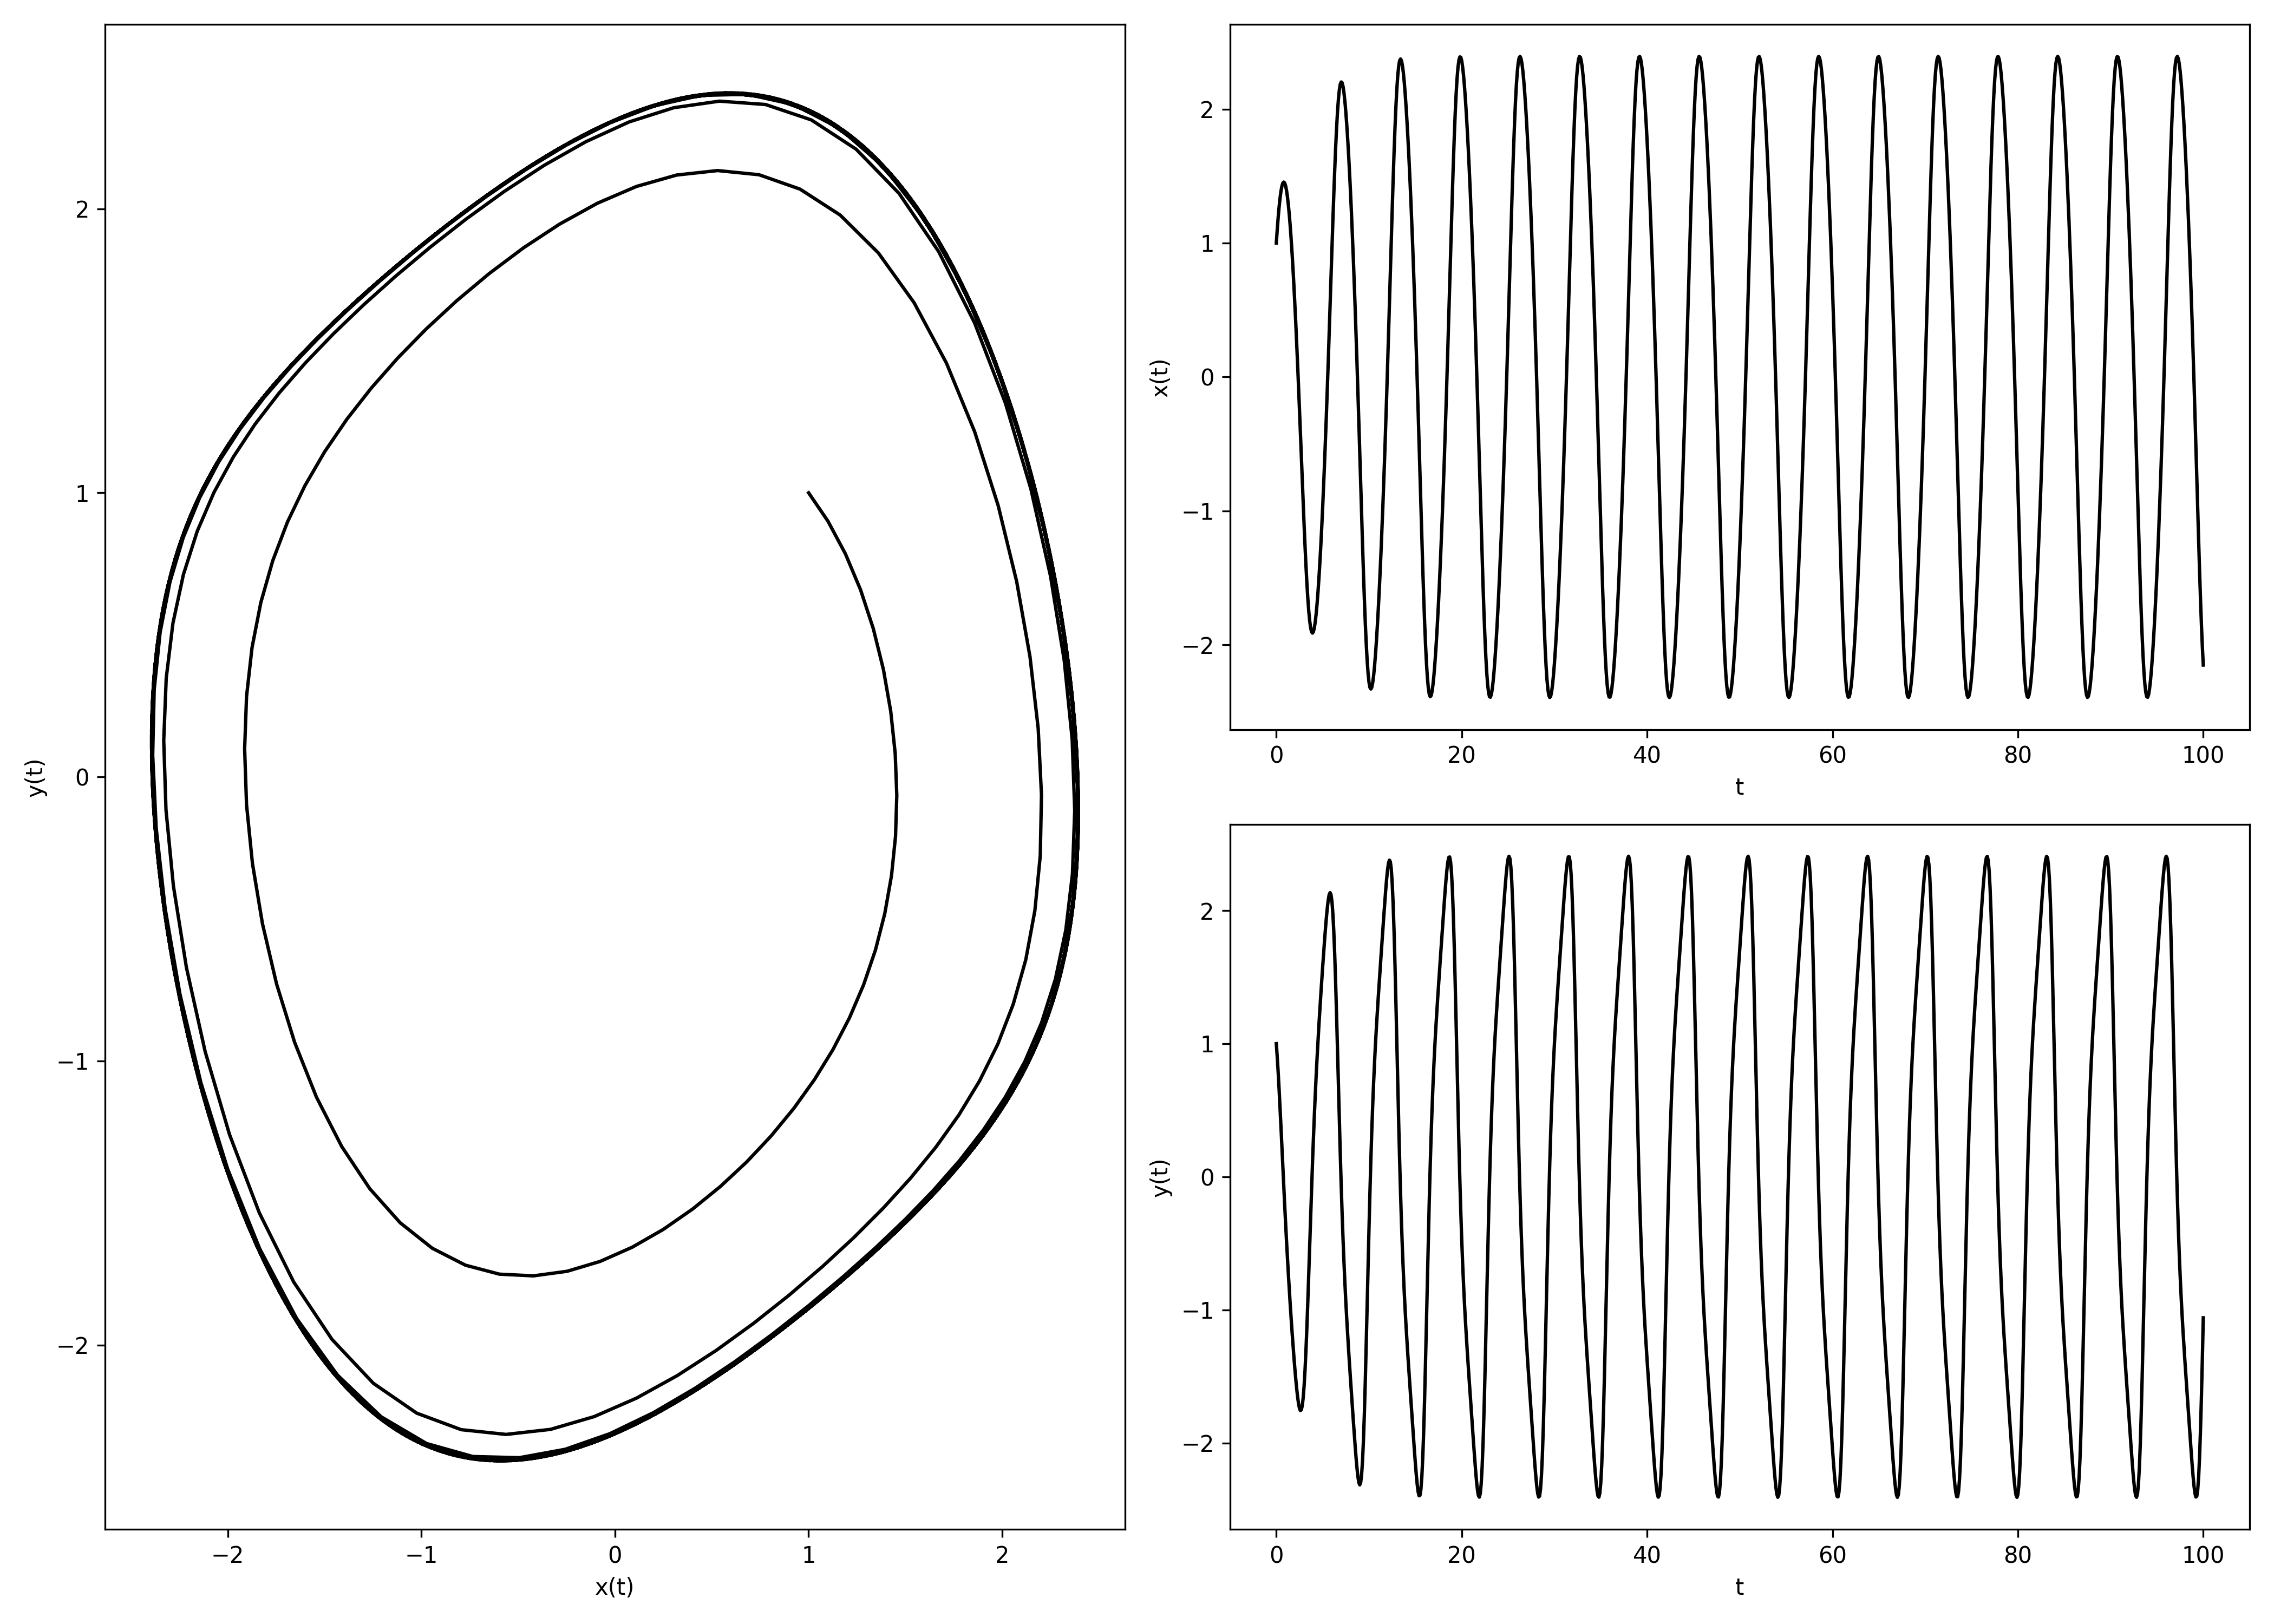
\includegraphics[scale=0.33]{x1,0y1,0mu0,2omega1,0t1,00e+02n1,00e+03.png}
% \figcaption{$x_0=1,00, y_0=1.00, \mu=0.25, \omega=1.00, T = 100, N = 1000$}
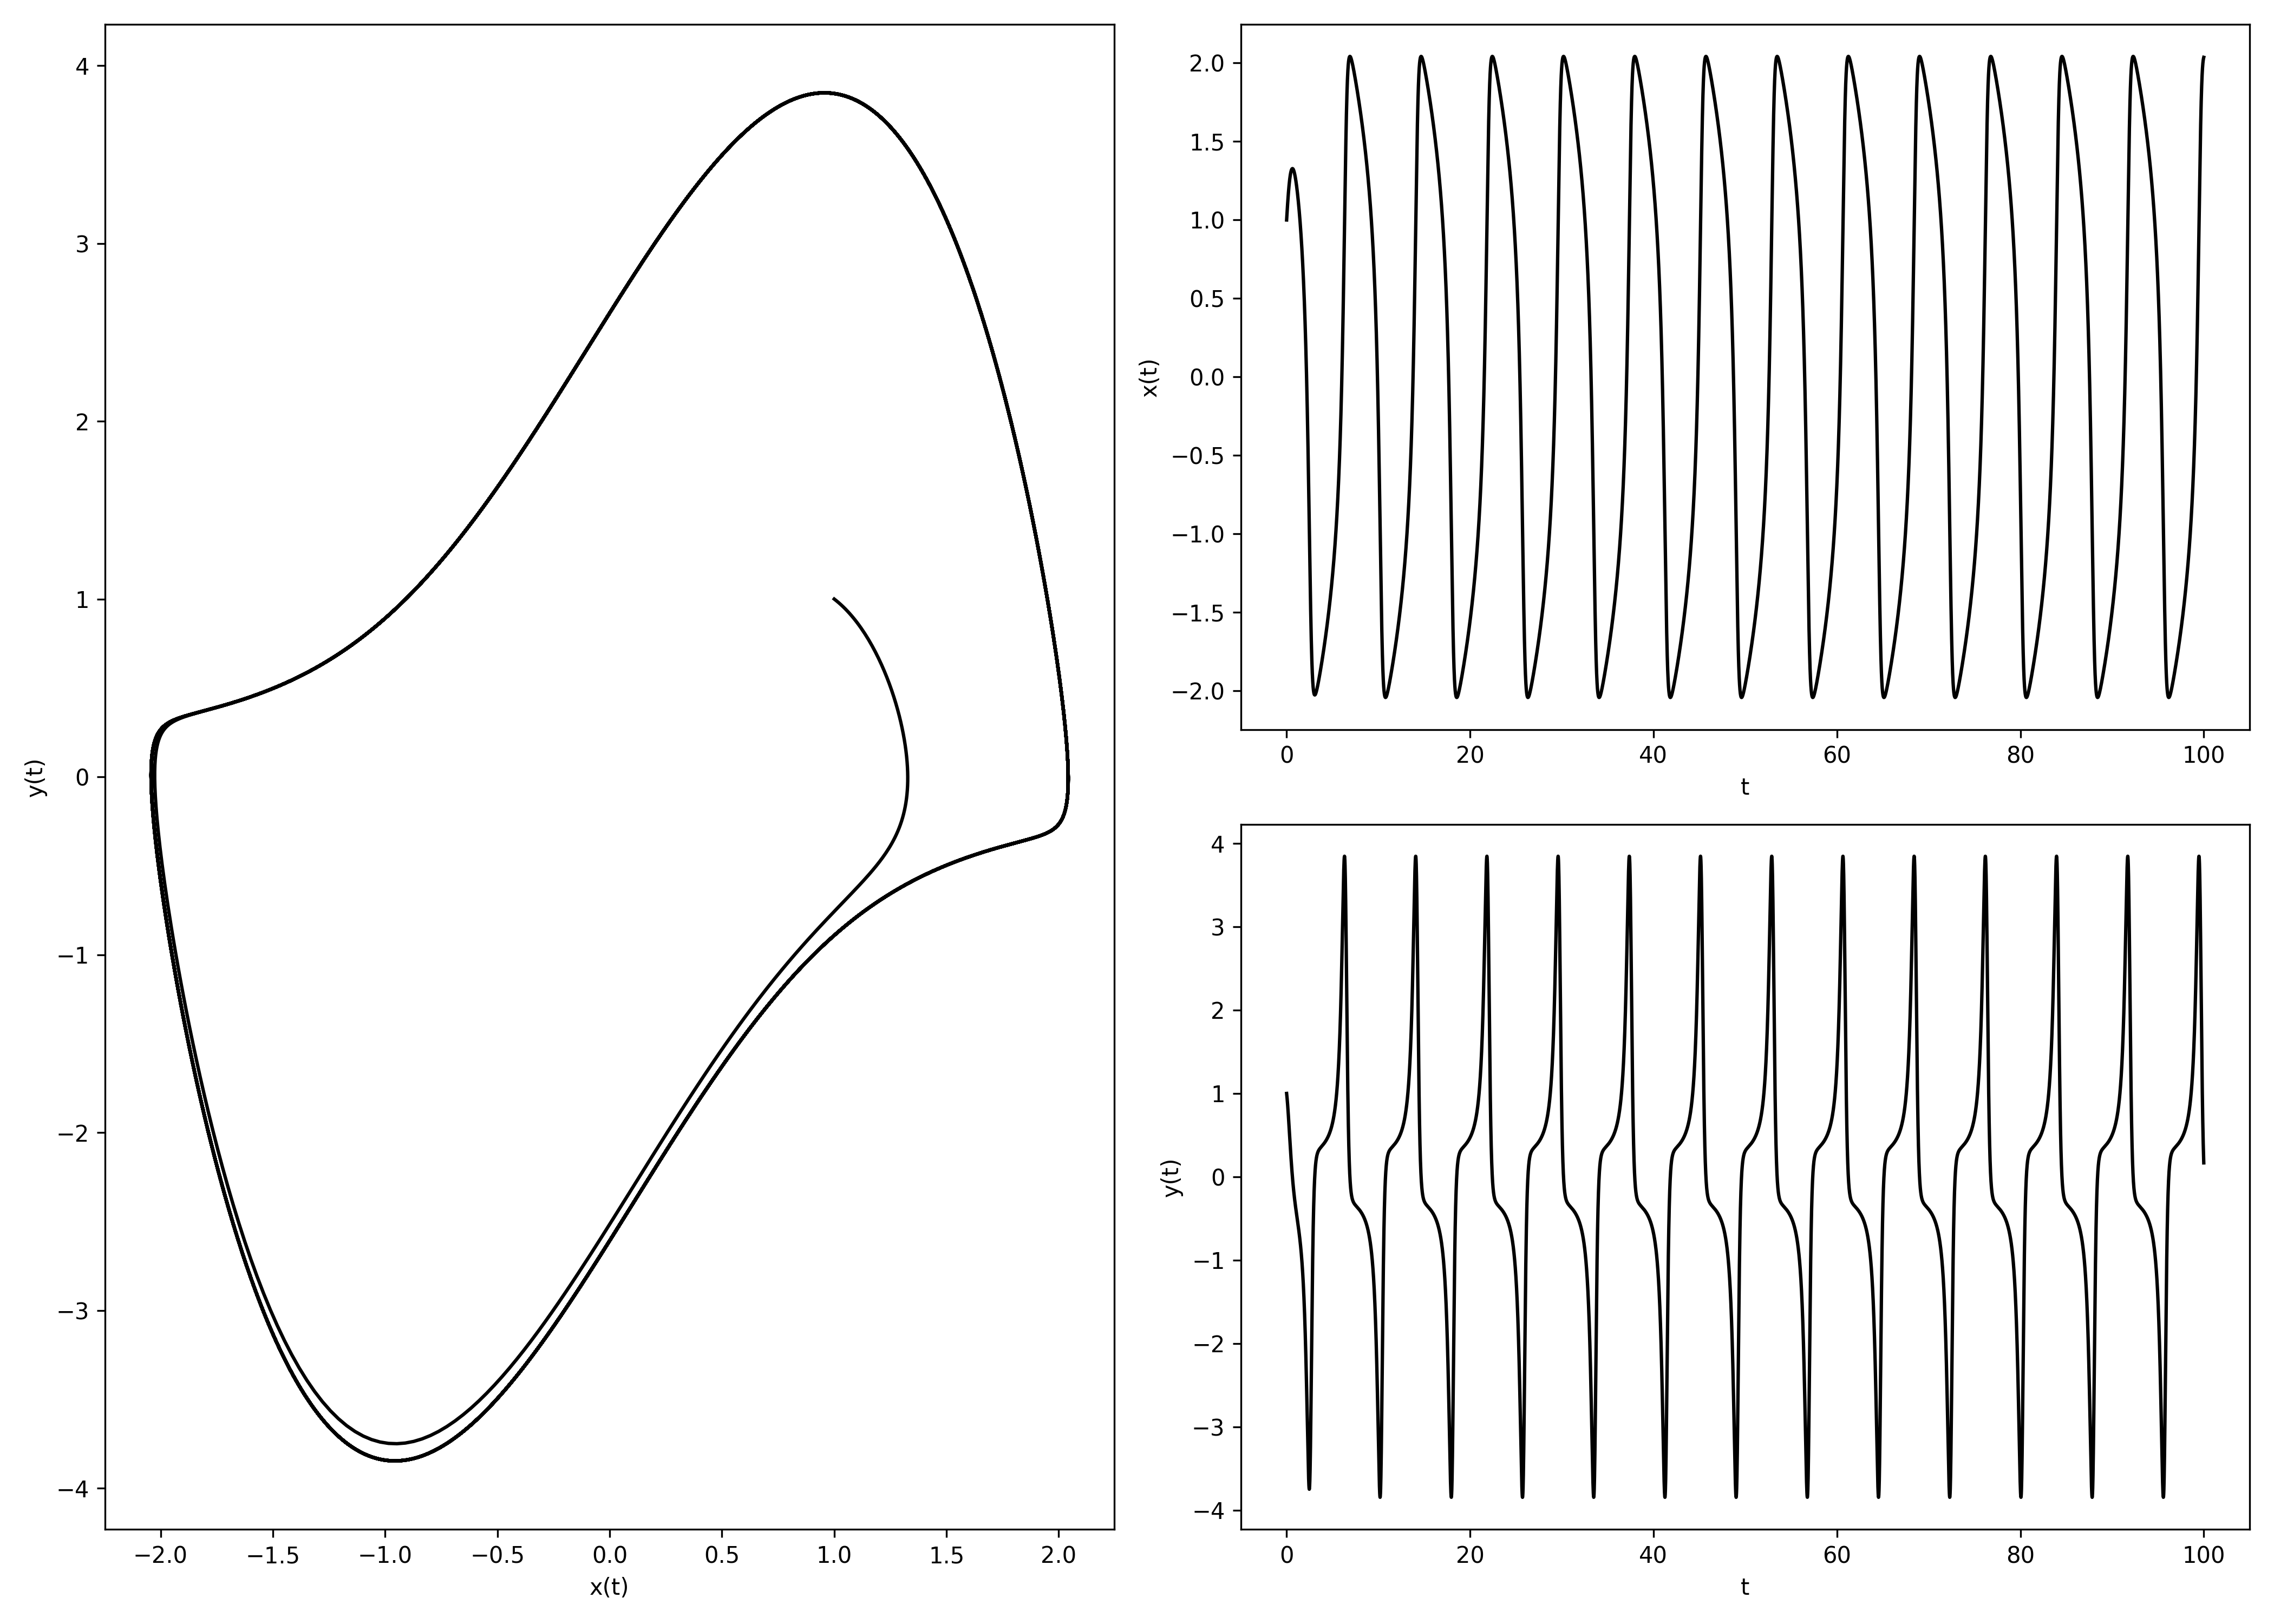
\includegraphics[scale=0.33]{x1,0y1,0mu2,0omega1,0t1,00e+02n1,00e+04.png}
\figcaption{$x_0=1,00, y_0=1.00, \mu=2.00, \omega=1.00, T = 100, N = 10000$}
%パラメーターomega
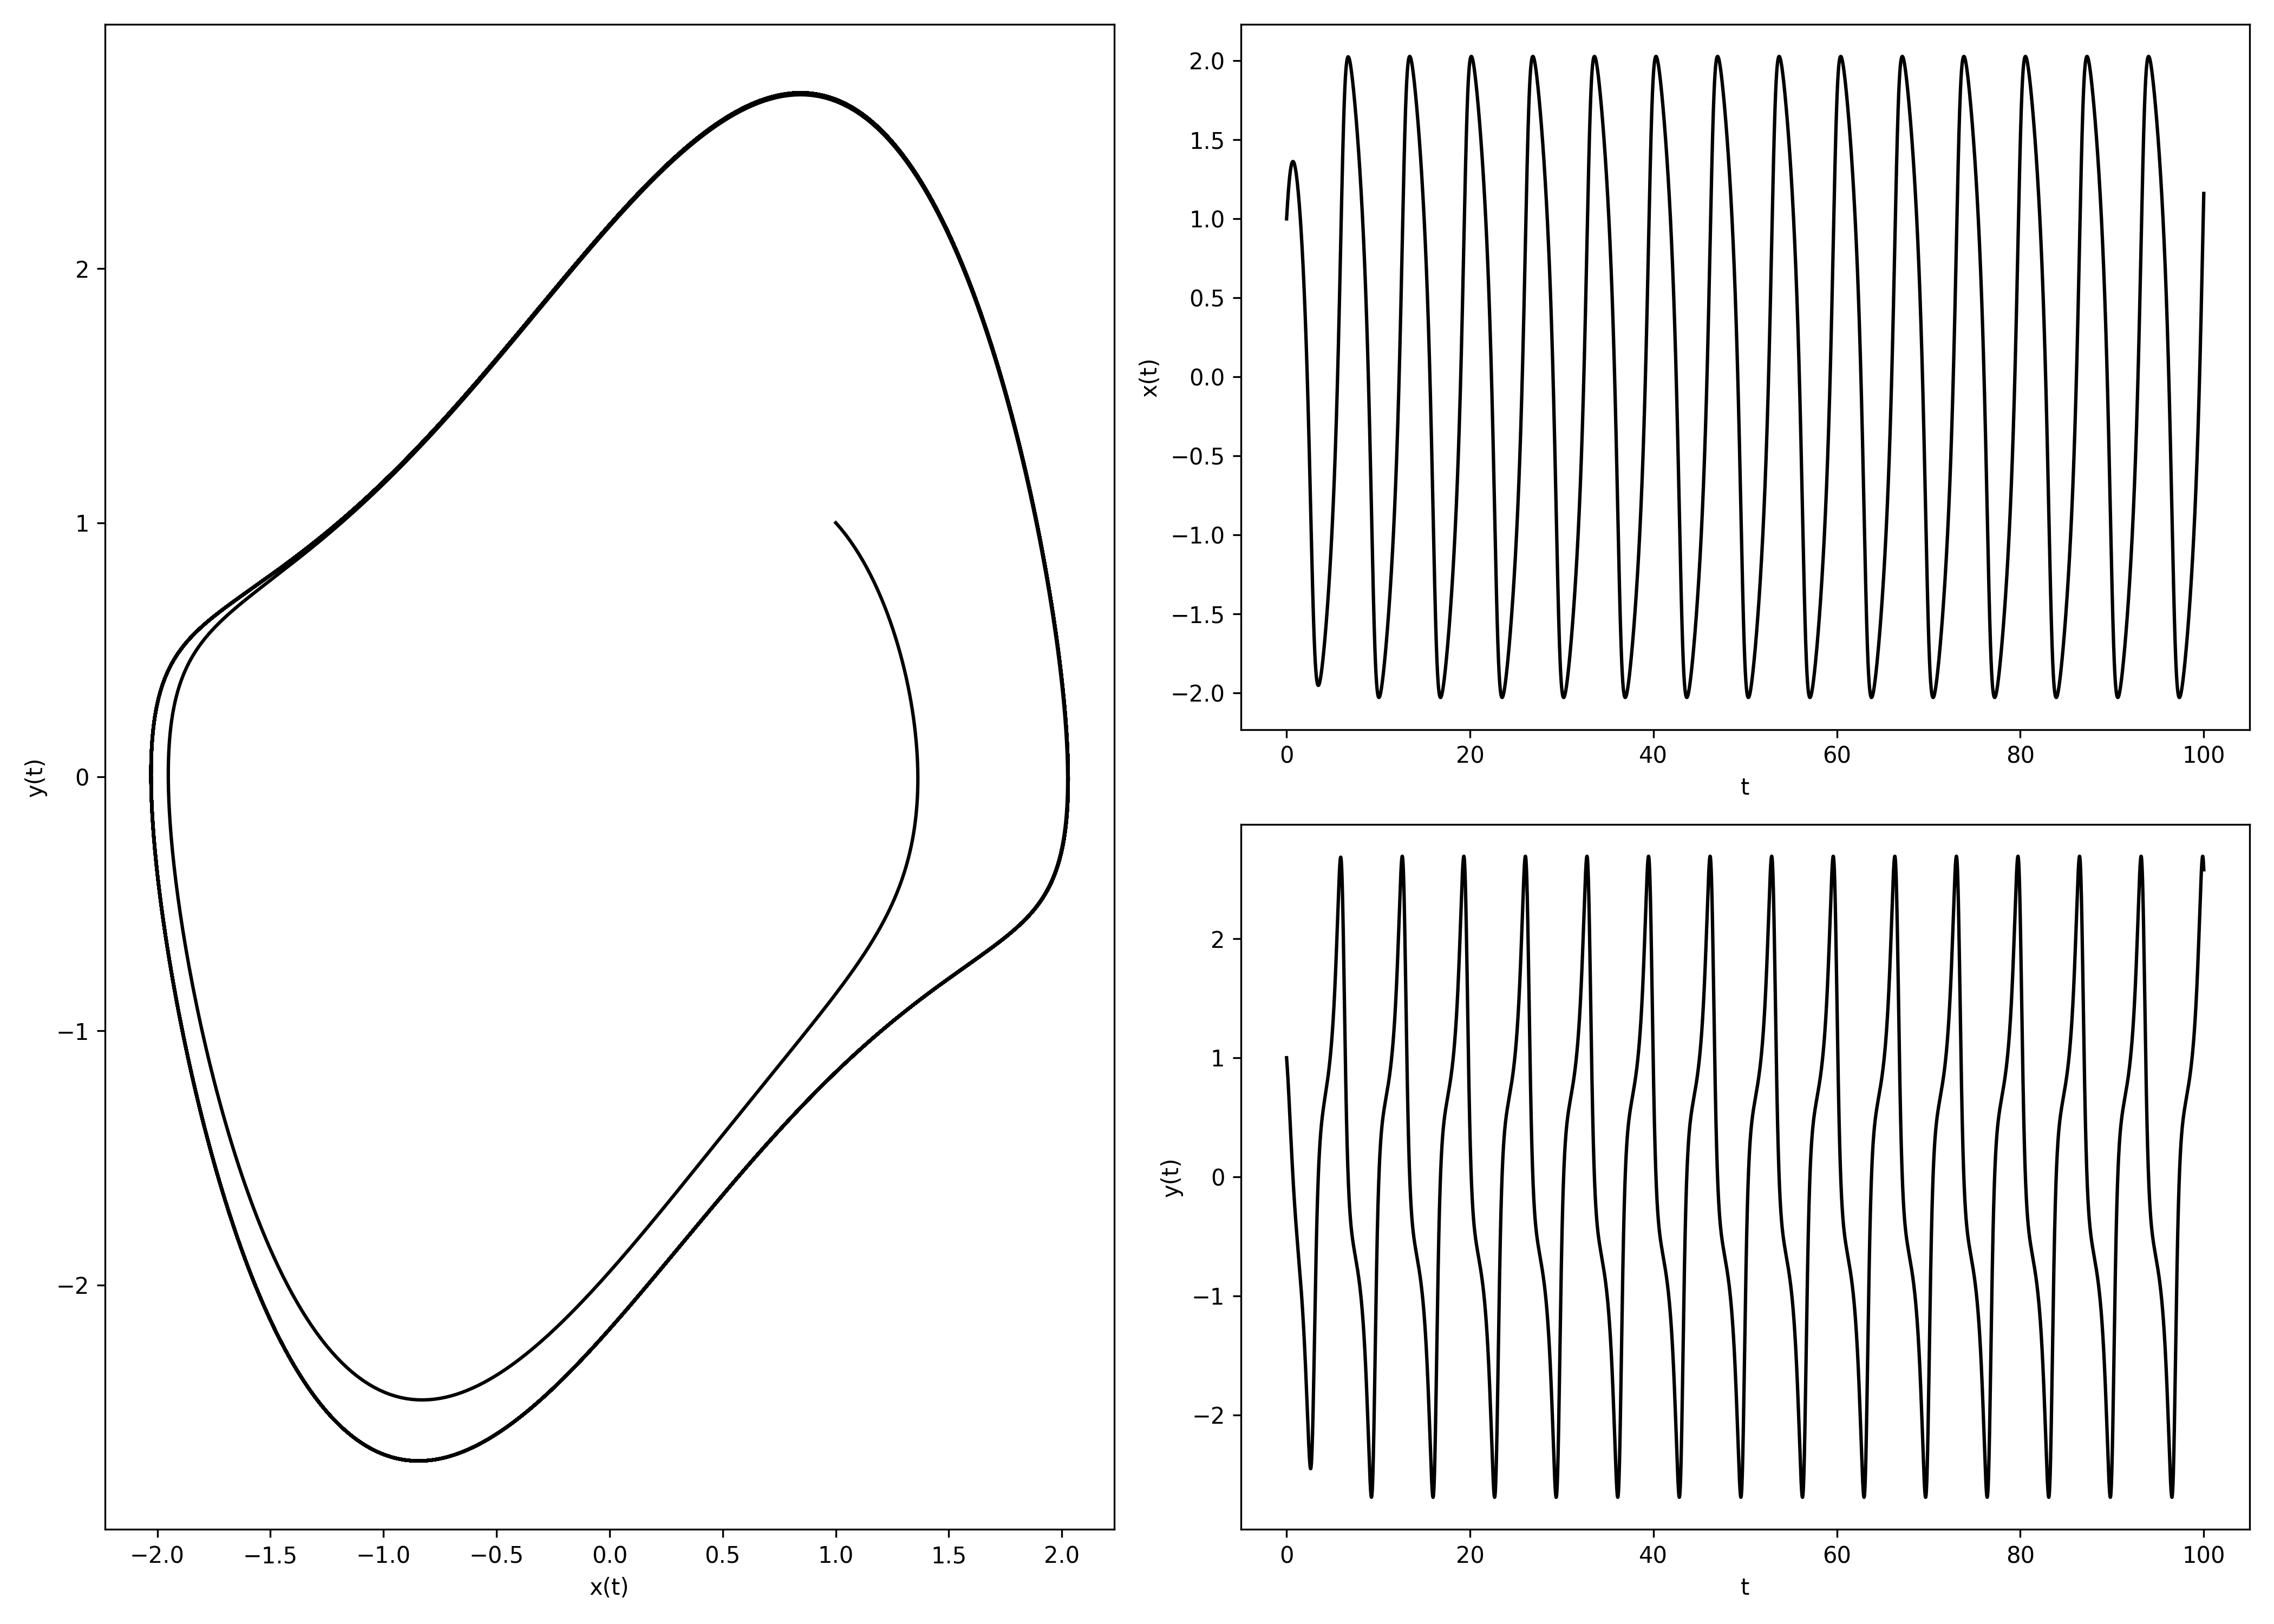
\includegraphics[scale=0.33]{x1,0y1,0mu1,0omega-1,0t1,00e+02n1,00e+04.png}
\figcaption{$x_0=1,00, y_0=1.00, \mu=1.00, \omega=-1.00, T = 100, N = 10000$}
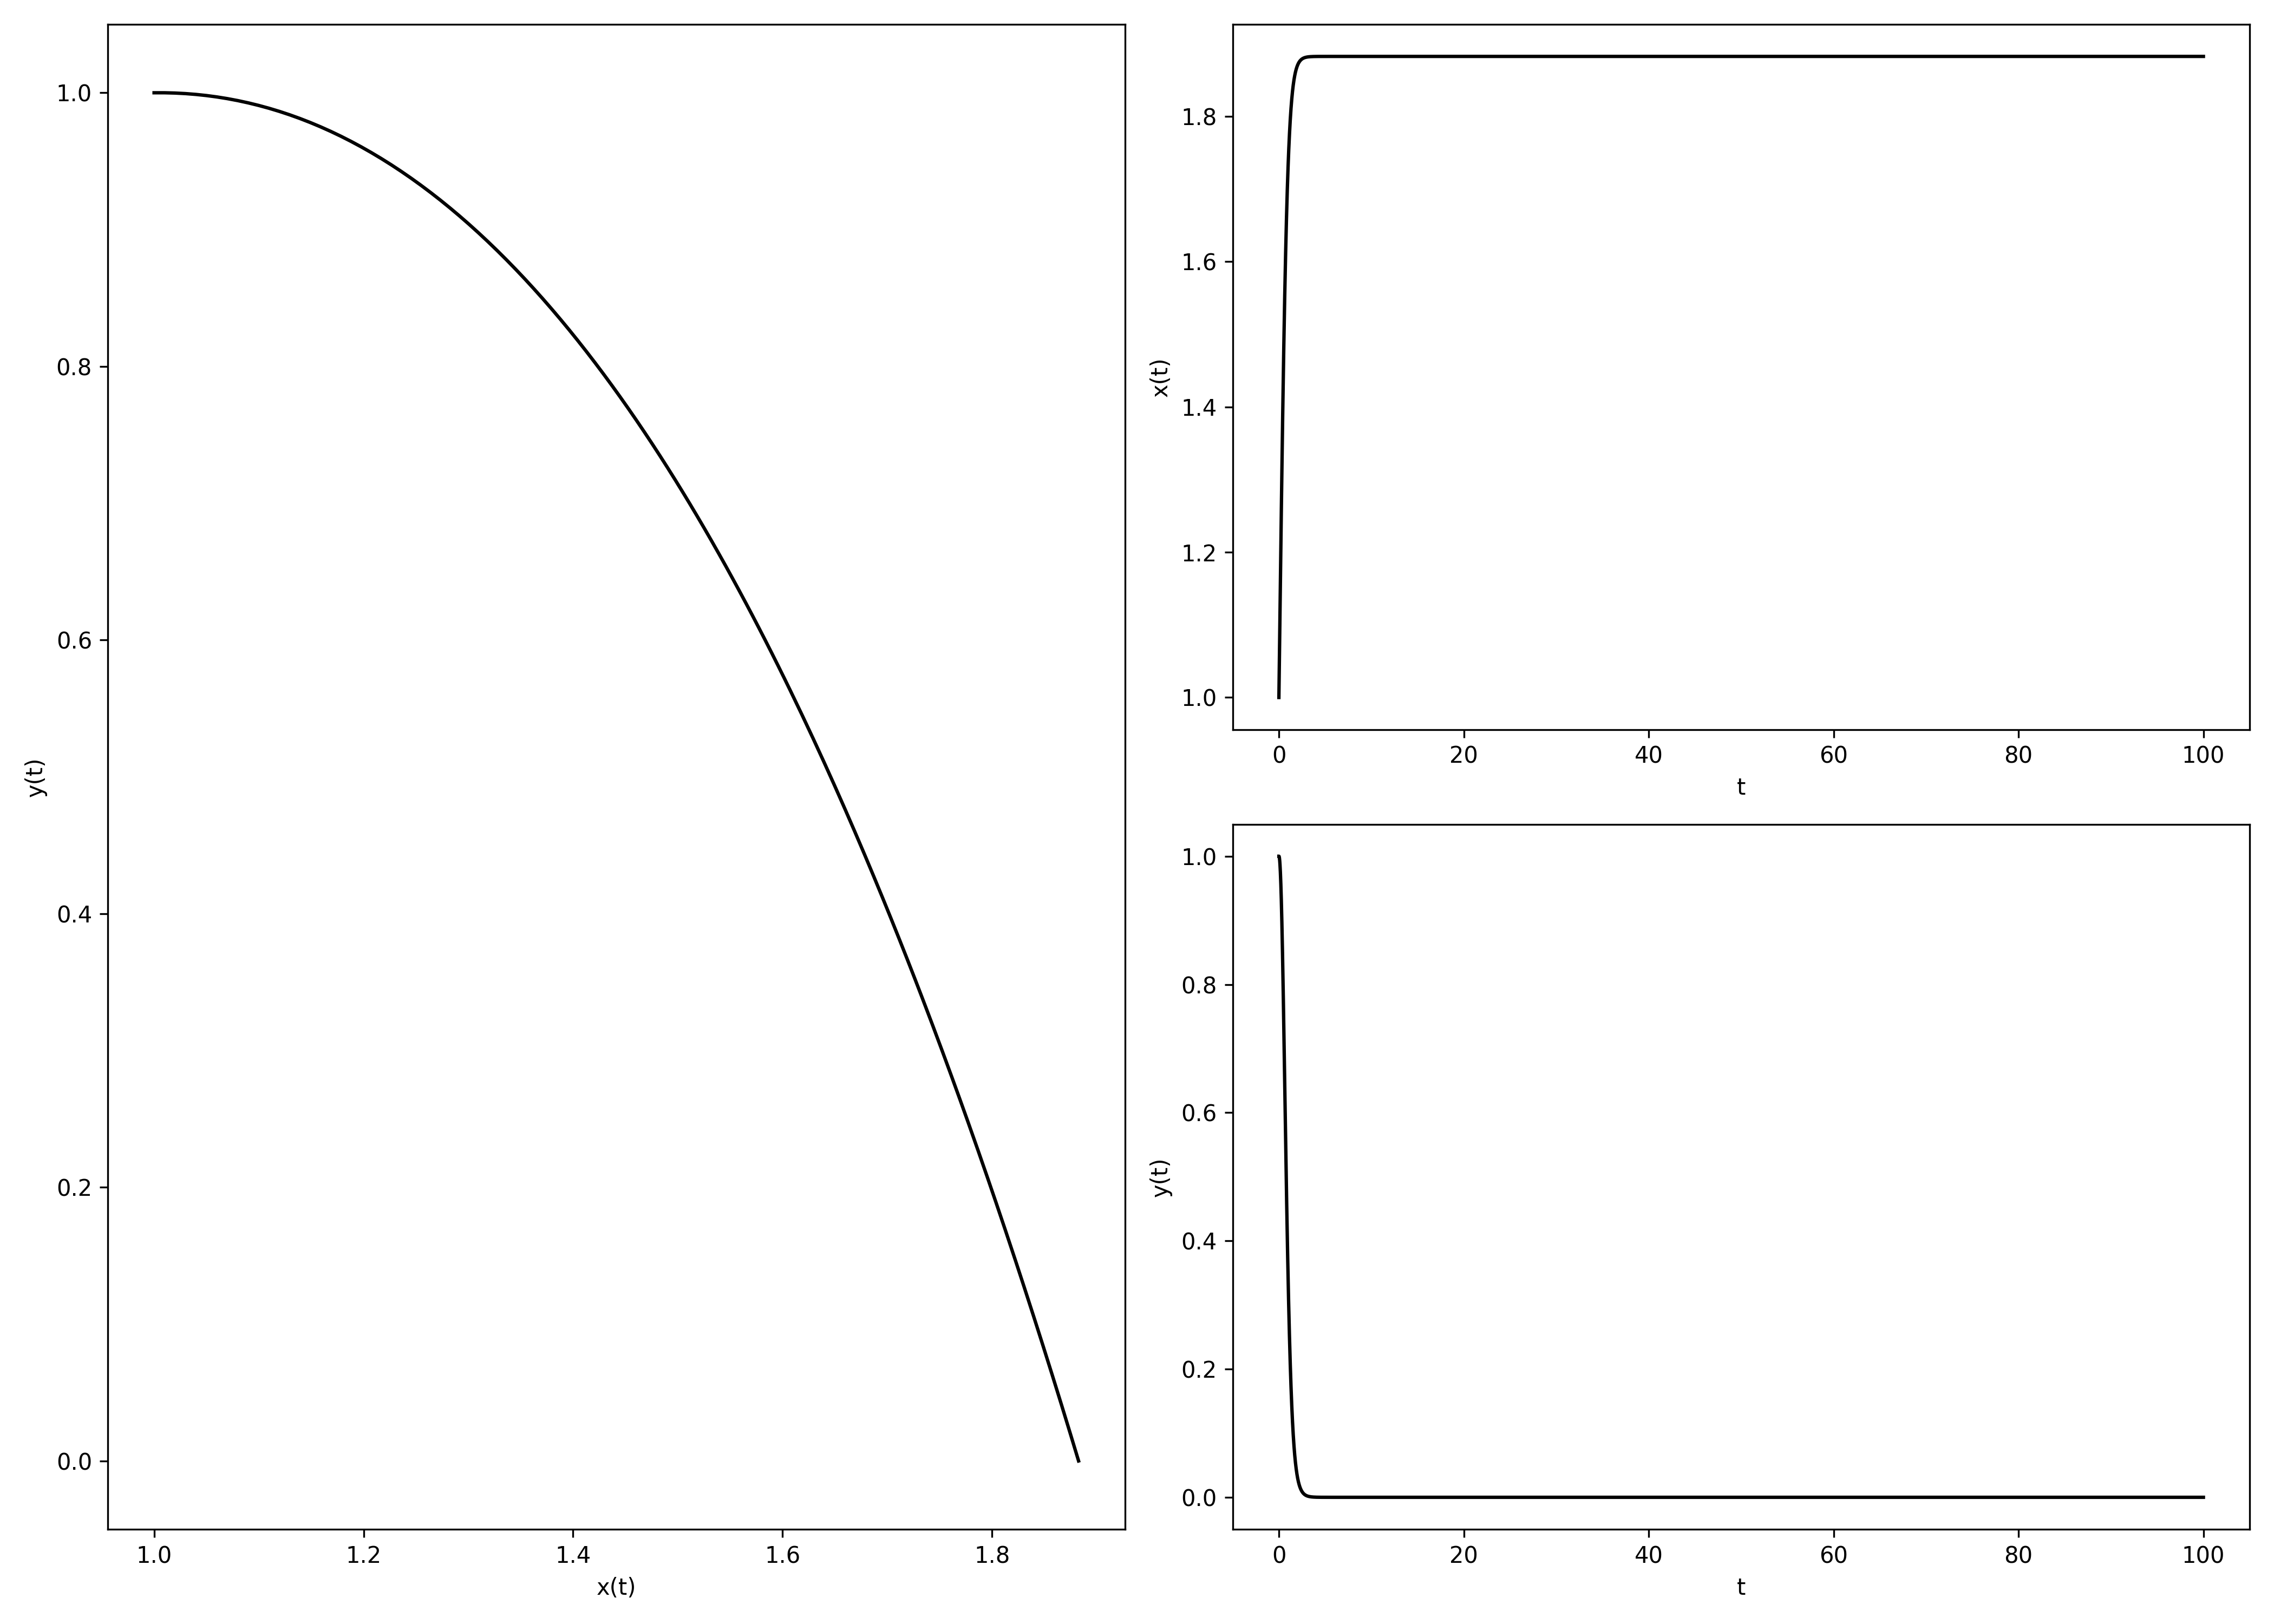
\includegraphics[scale=0.33]{x1,0y1,0mu1,0omega0,0t1,00e+02n1,00e+04.png}
\figcaption{$x_0=1,00, y_0=1.00, \mu=1.00, \omega=0.00, T = 100, N = 10000$}
% 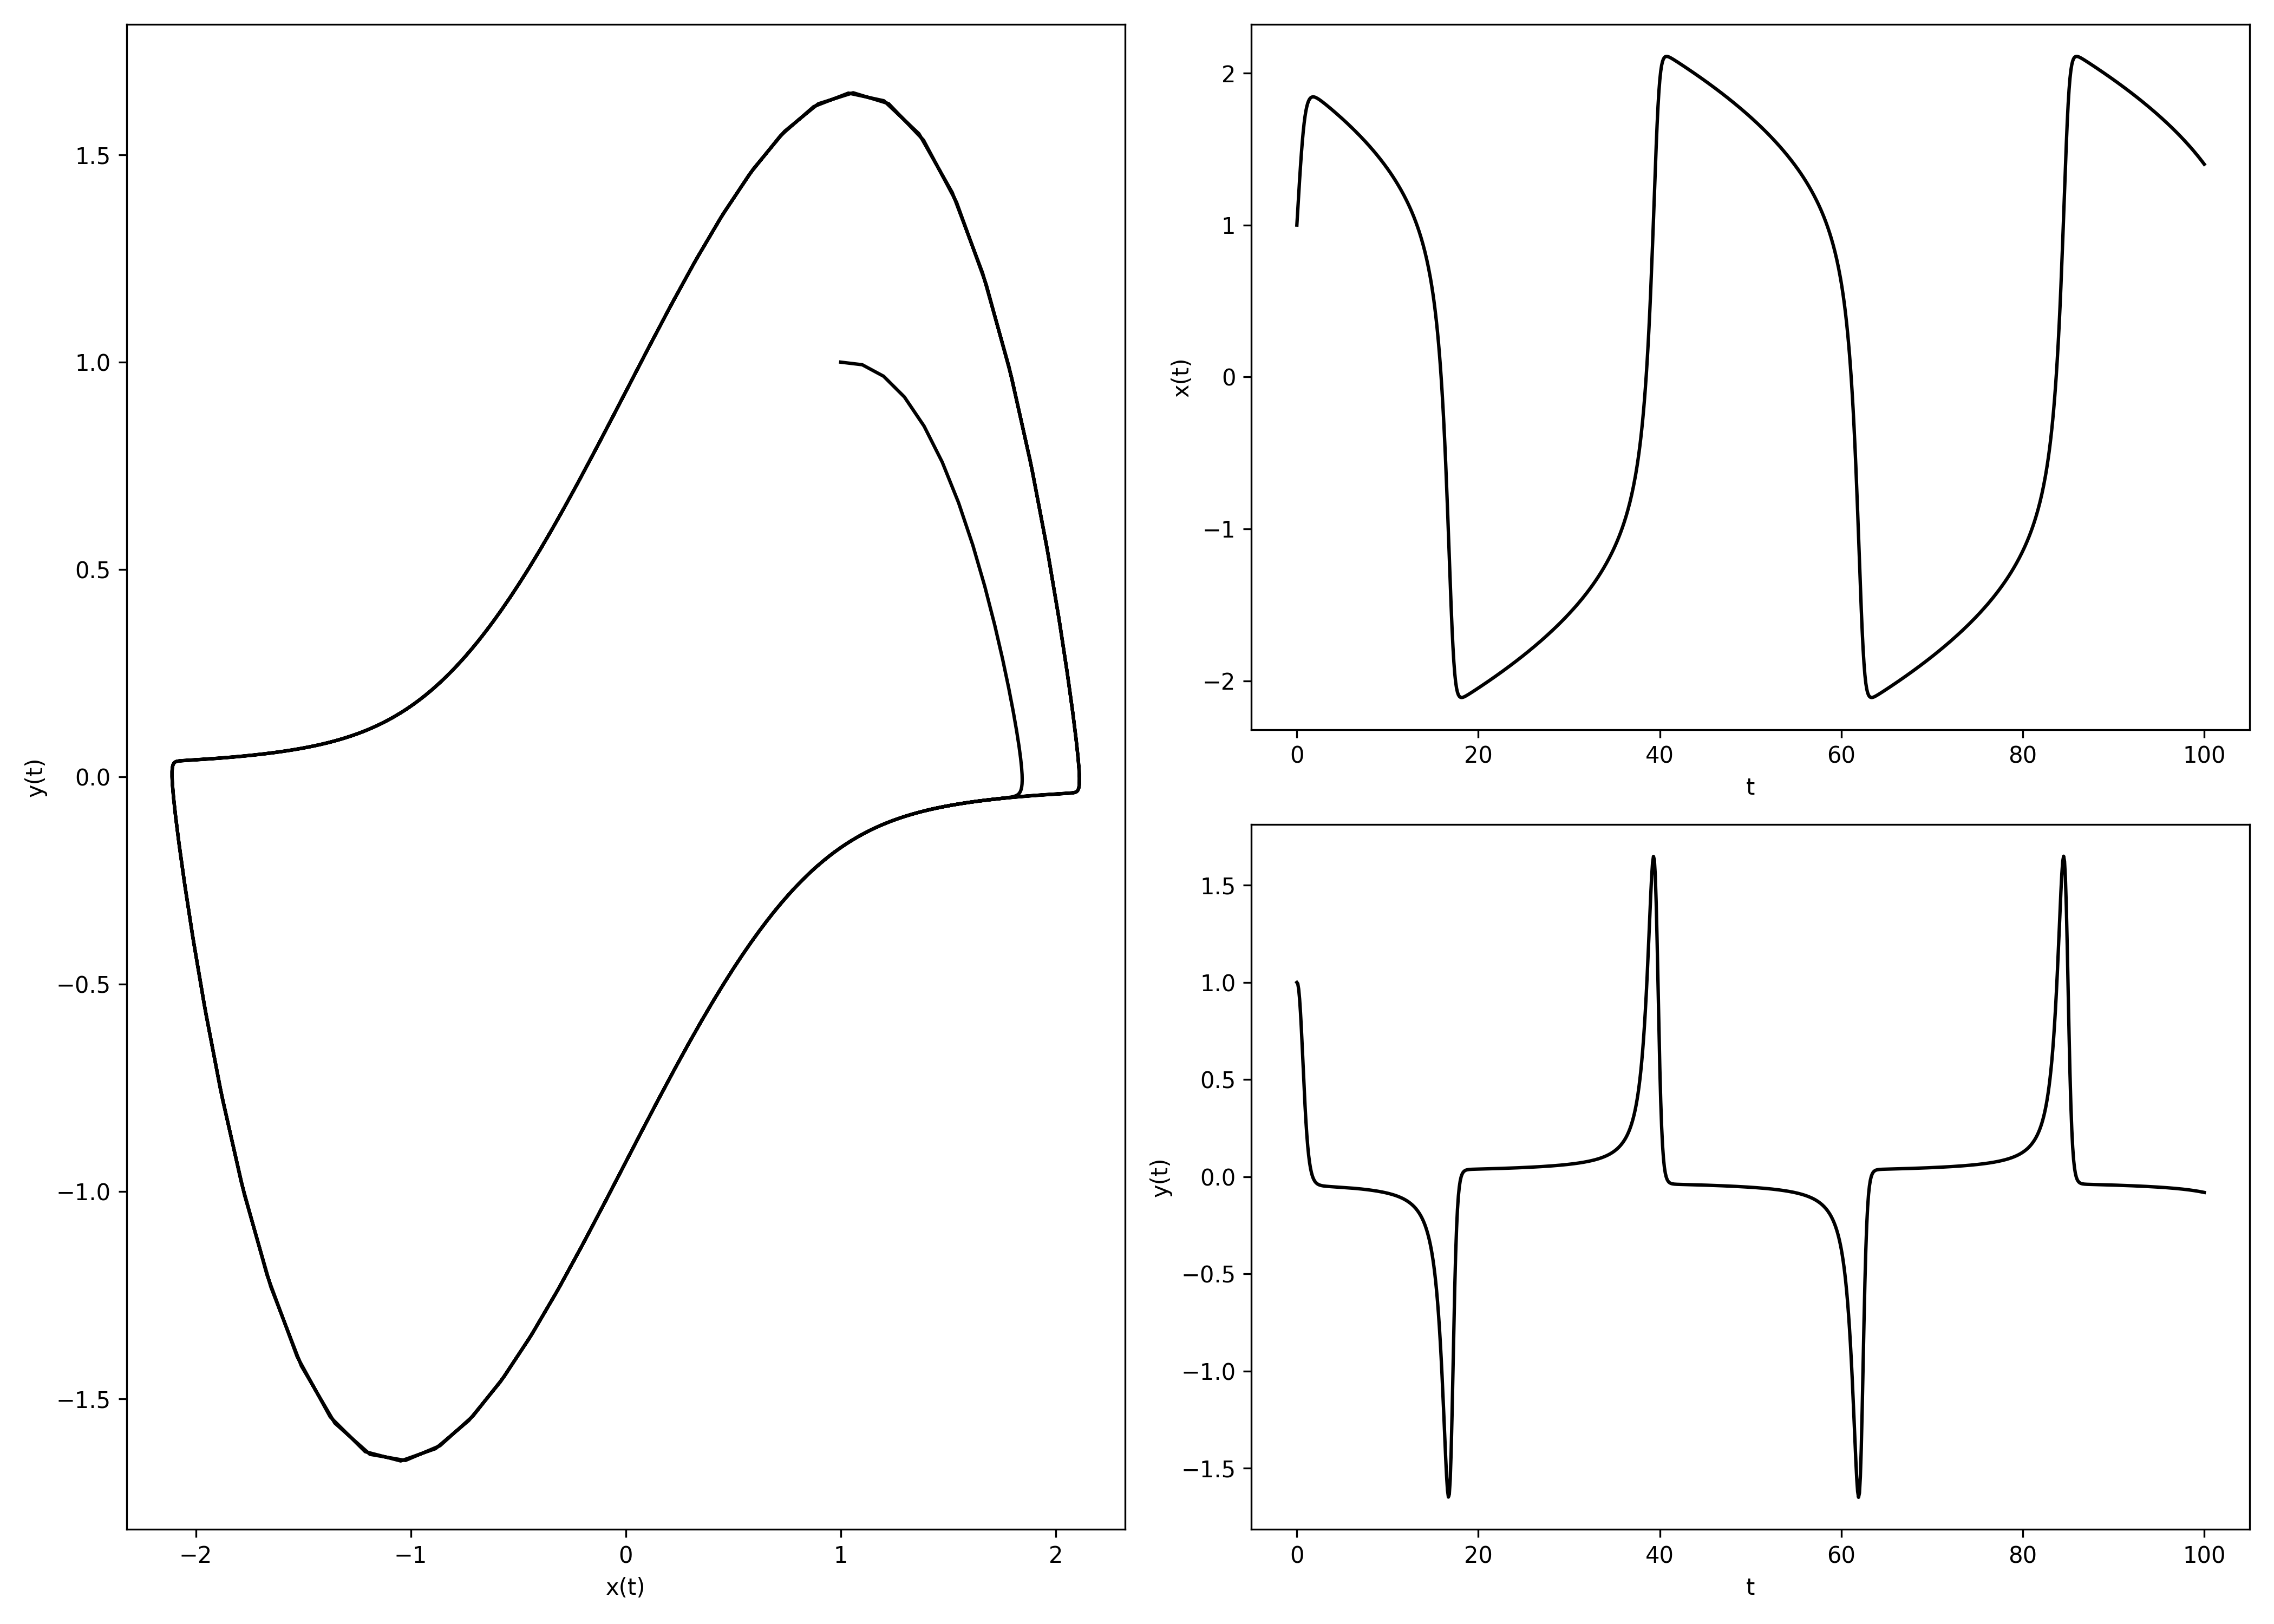
\includegraphics[scale=0.33]{x1,0y1,0mu1,0omega0,2t1,00e+02n1,00e+03.png}
% \figcaption{$x_0=1,00, y_0=1.00, \mu=1.00, \omega=0.25, T = 100, N = 1000$}
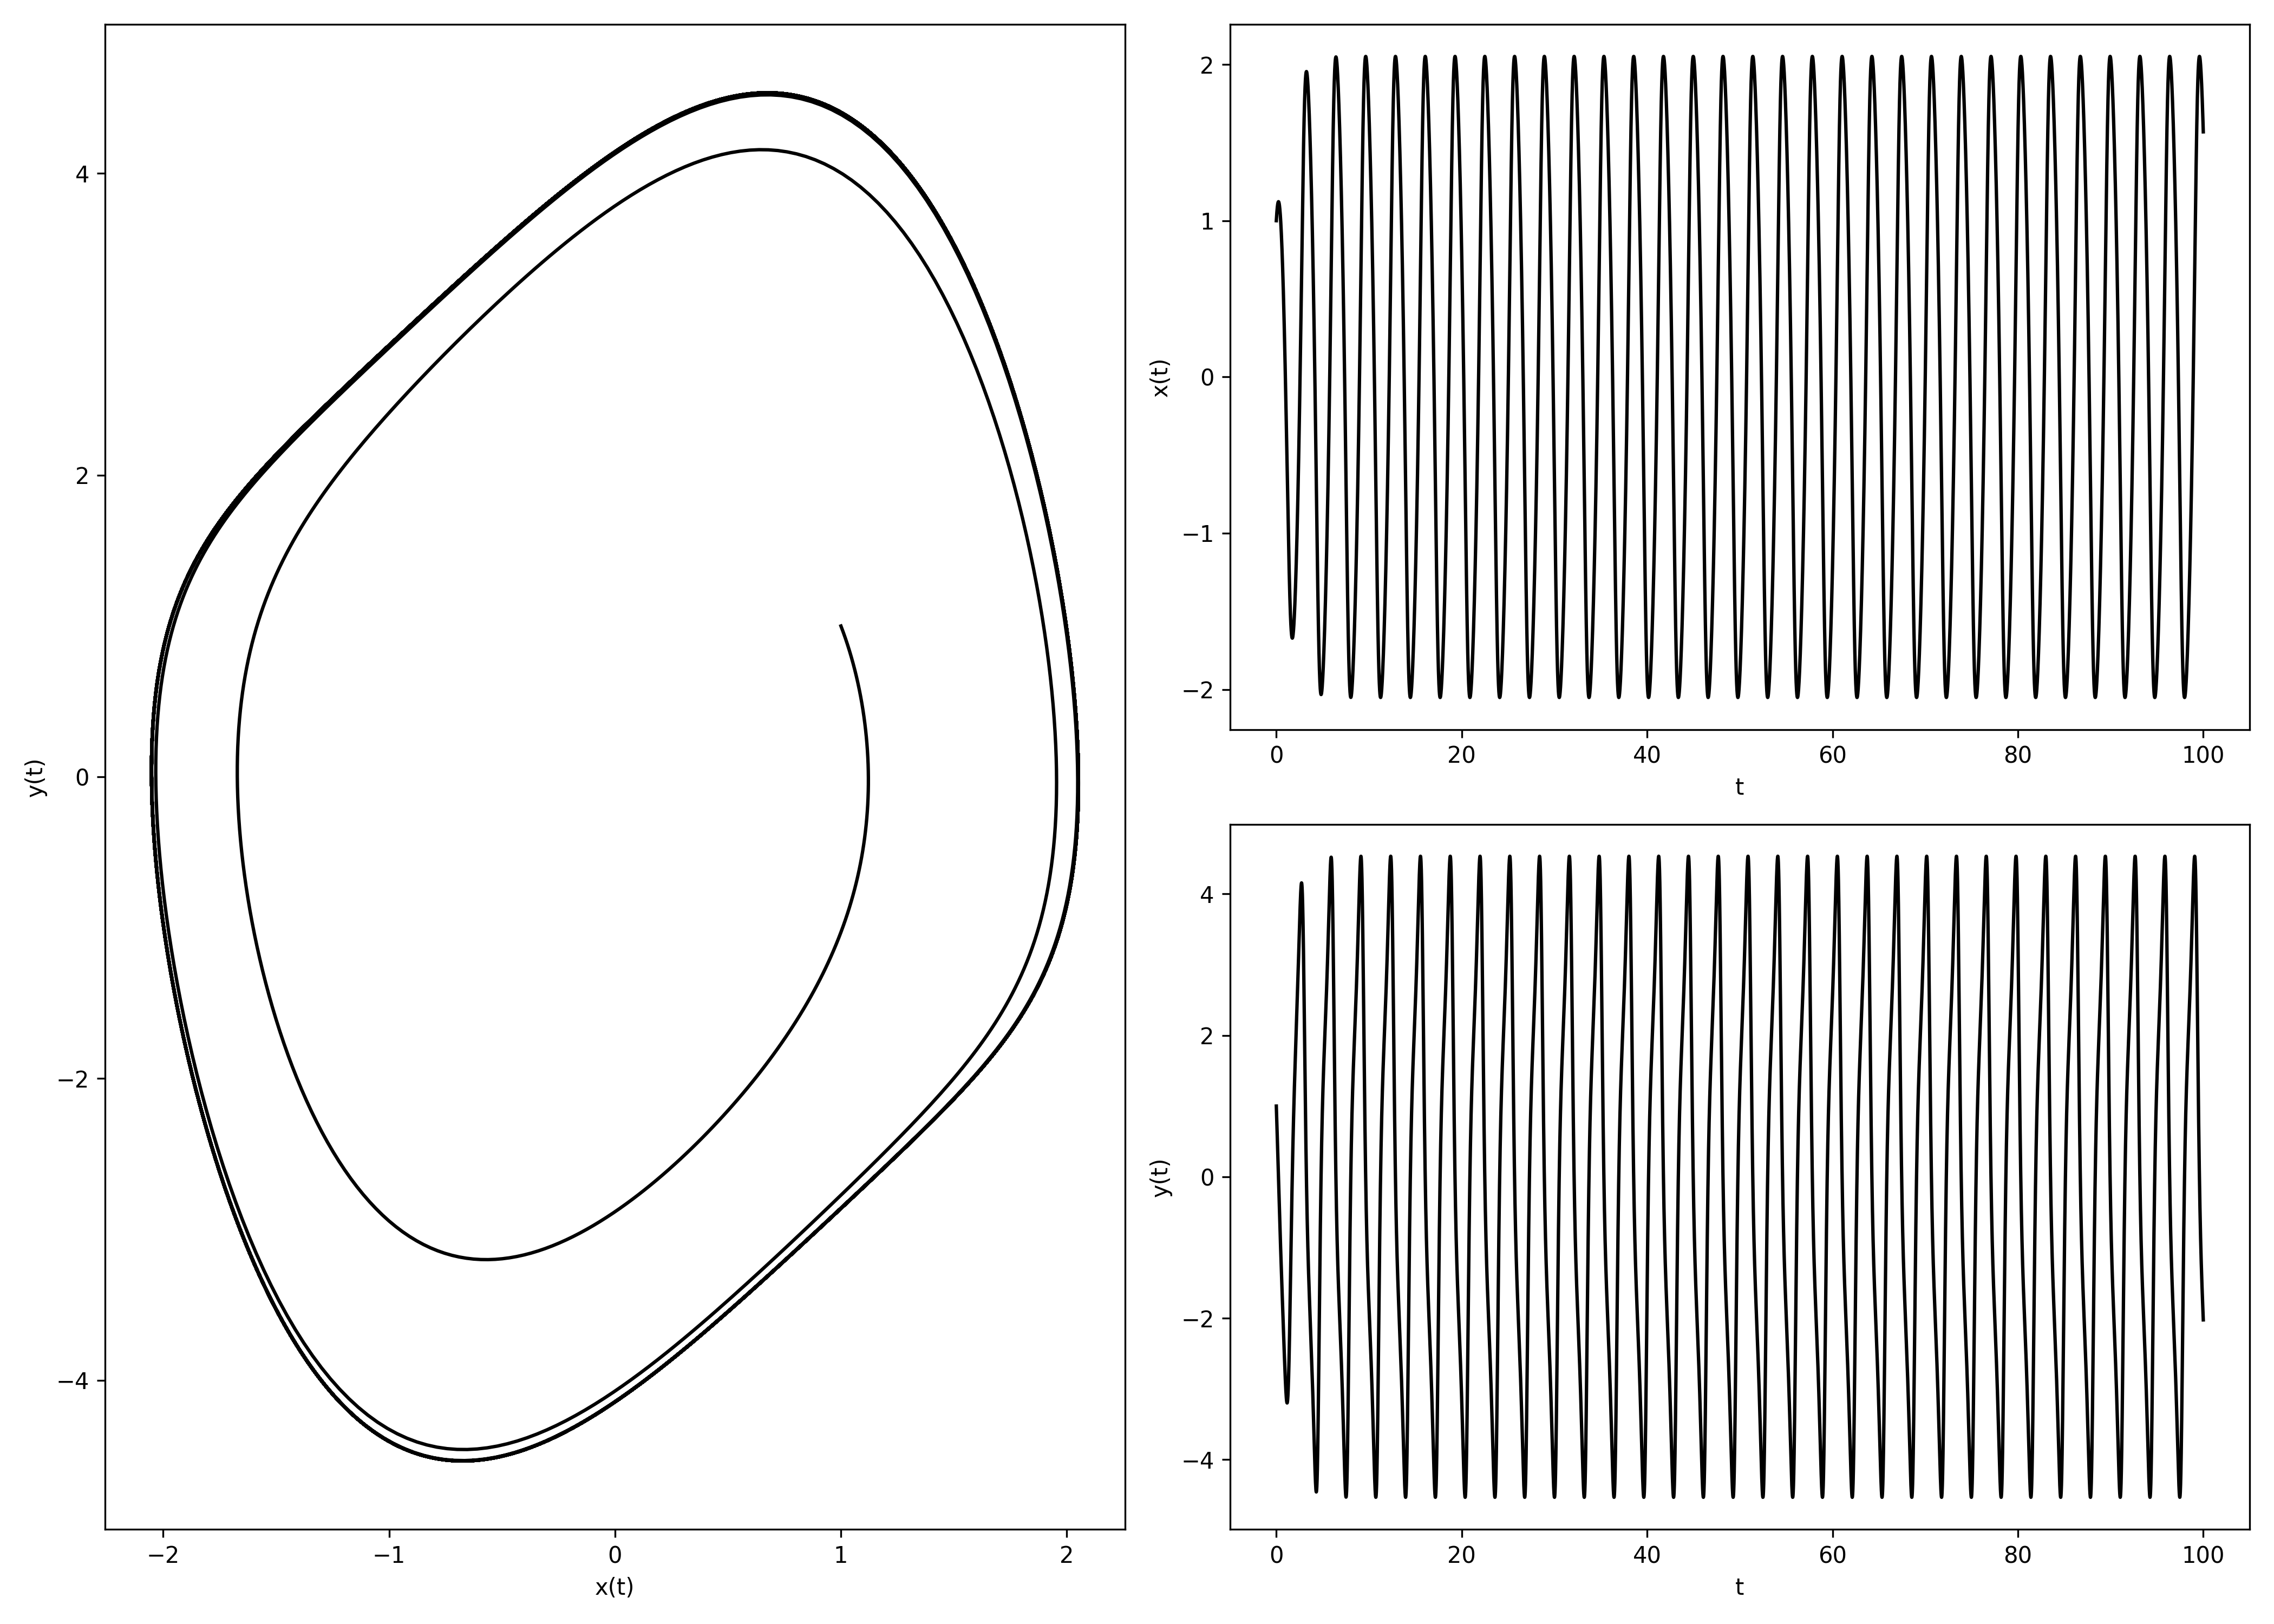
\includegraphics[scale=0.33]{x1,0y1,0mu1,0omega2,0t1,00e+02n1,00e+04.png}
\figcaption{$x_0=1,00, y_0=1.00, \mu=1.00, \omega=2.00, T = 100, N = 10000$}
%パラメーター初期値
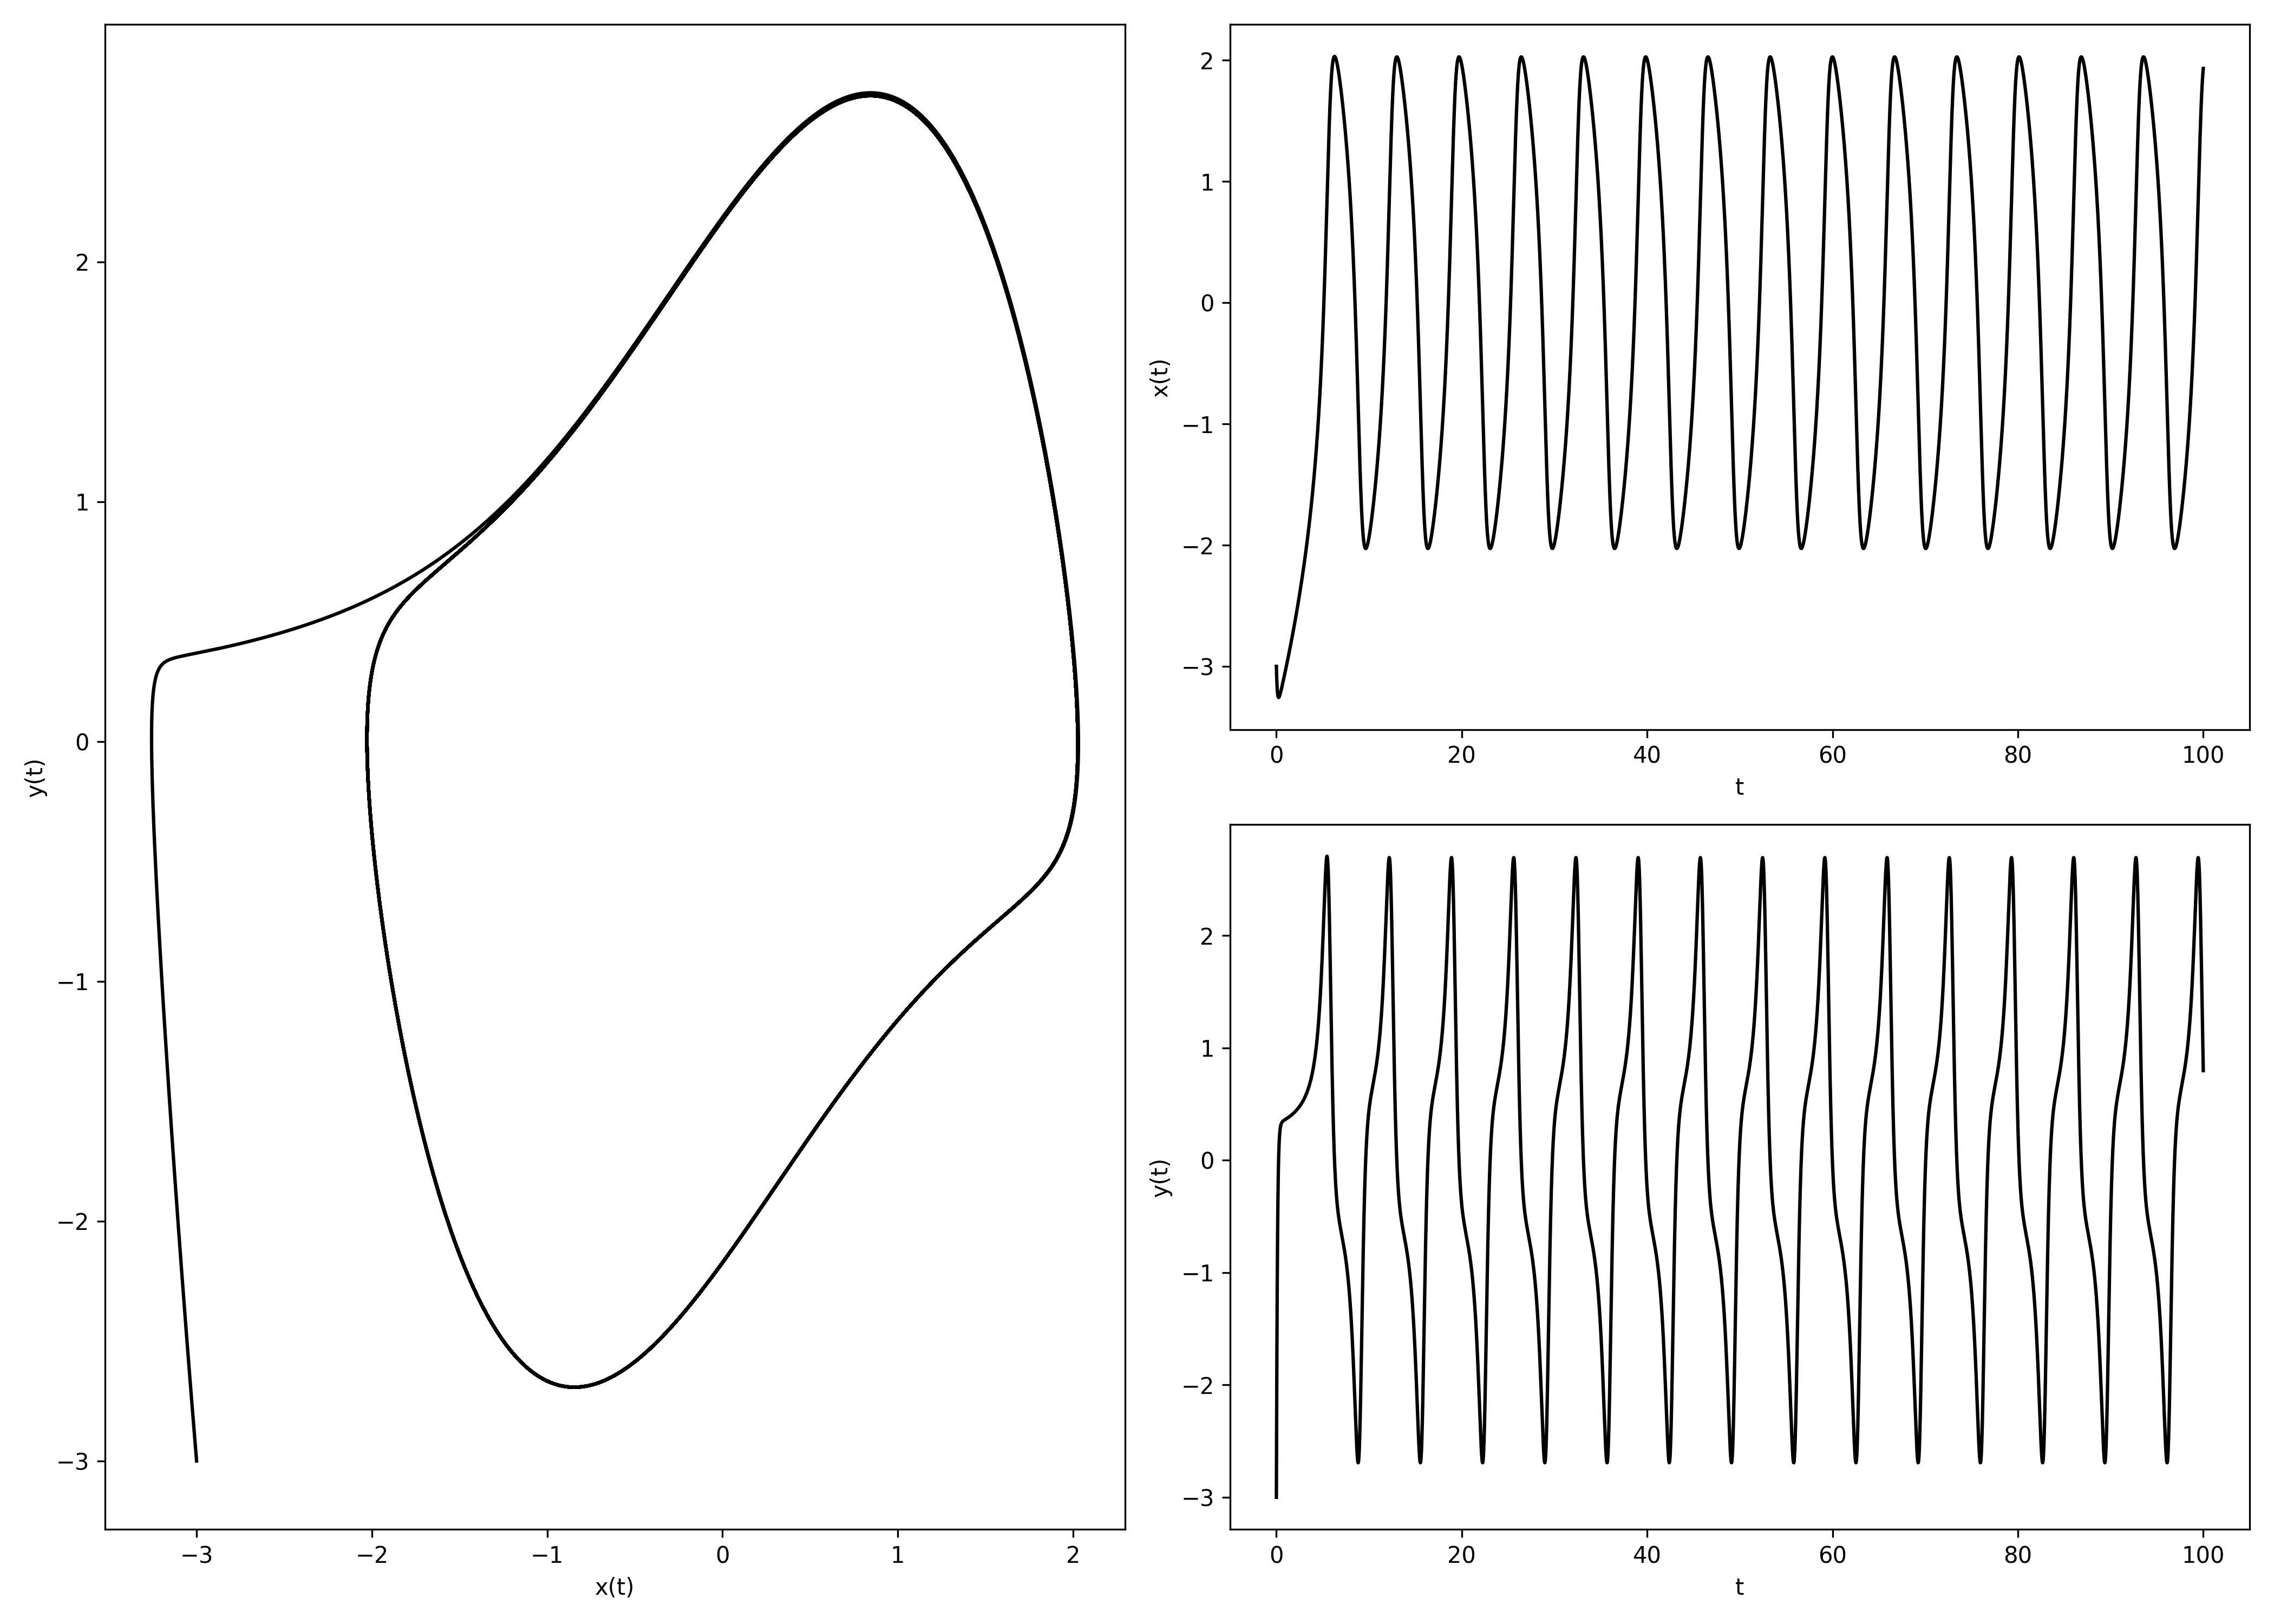
\includegraphics[scale=0.33]{x-3,0y-3,0mu1,0omega1,0t1,00e+02n1,00e+04.png}
\figcaption{$x_0=-3.00, y_0=-3.00, \mu=1,00, \omega=1.00, T = 100, N = 10000$}
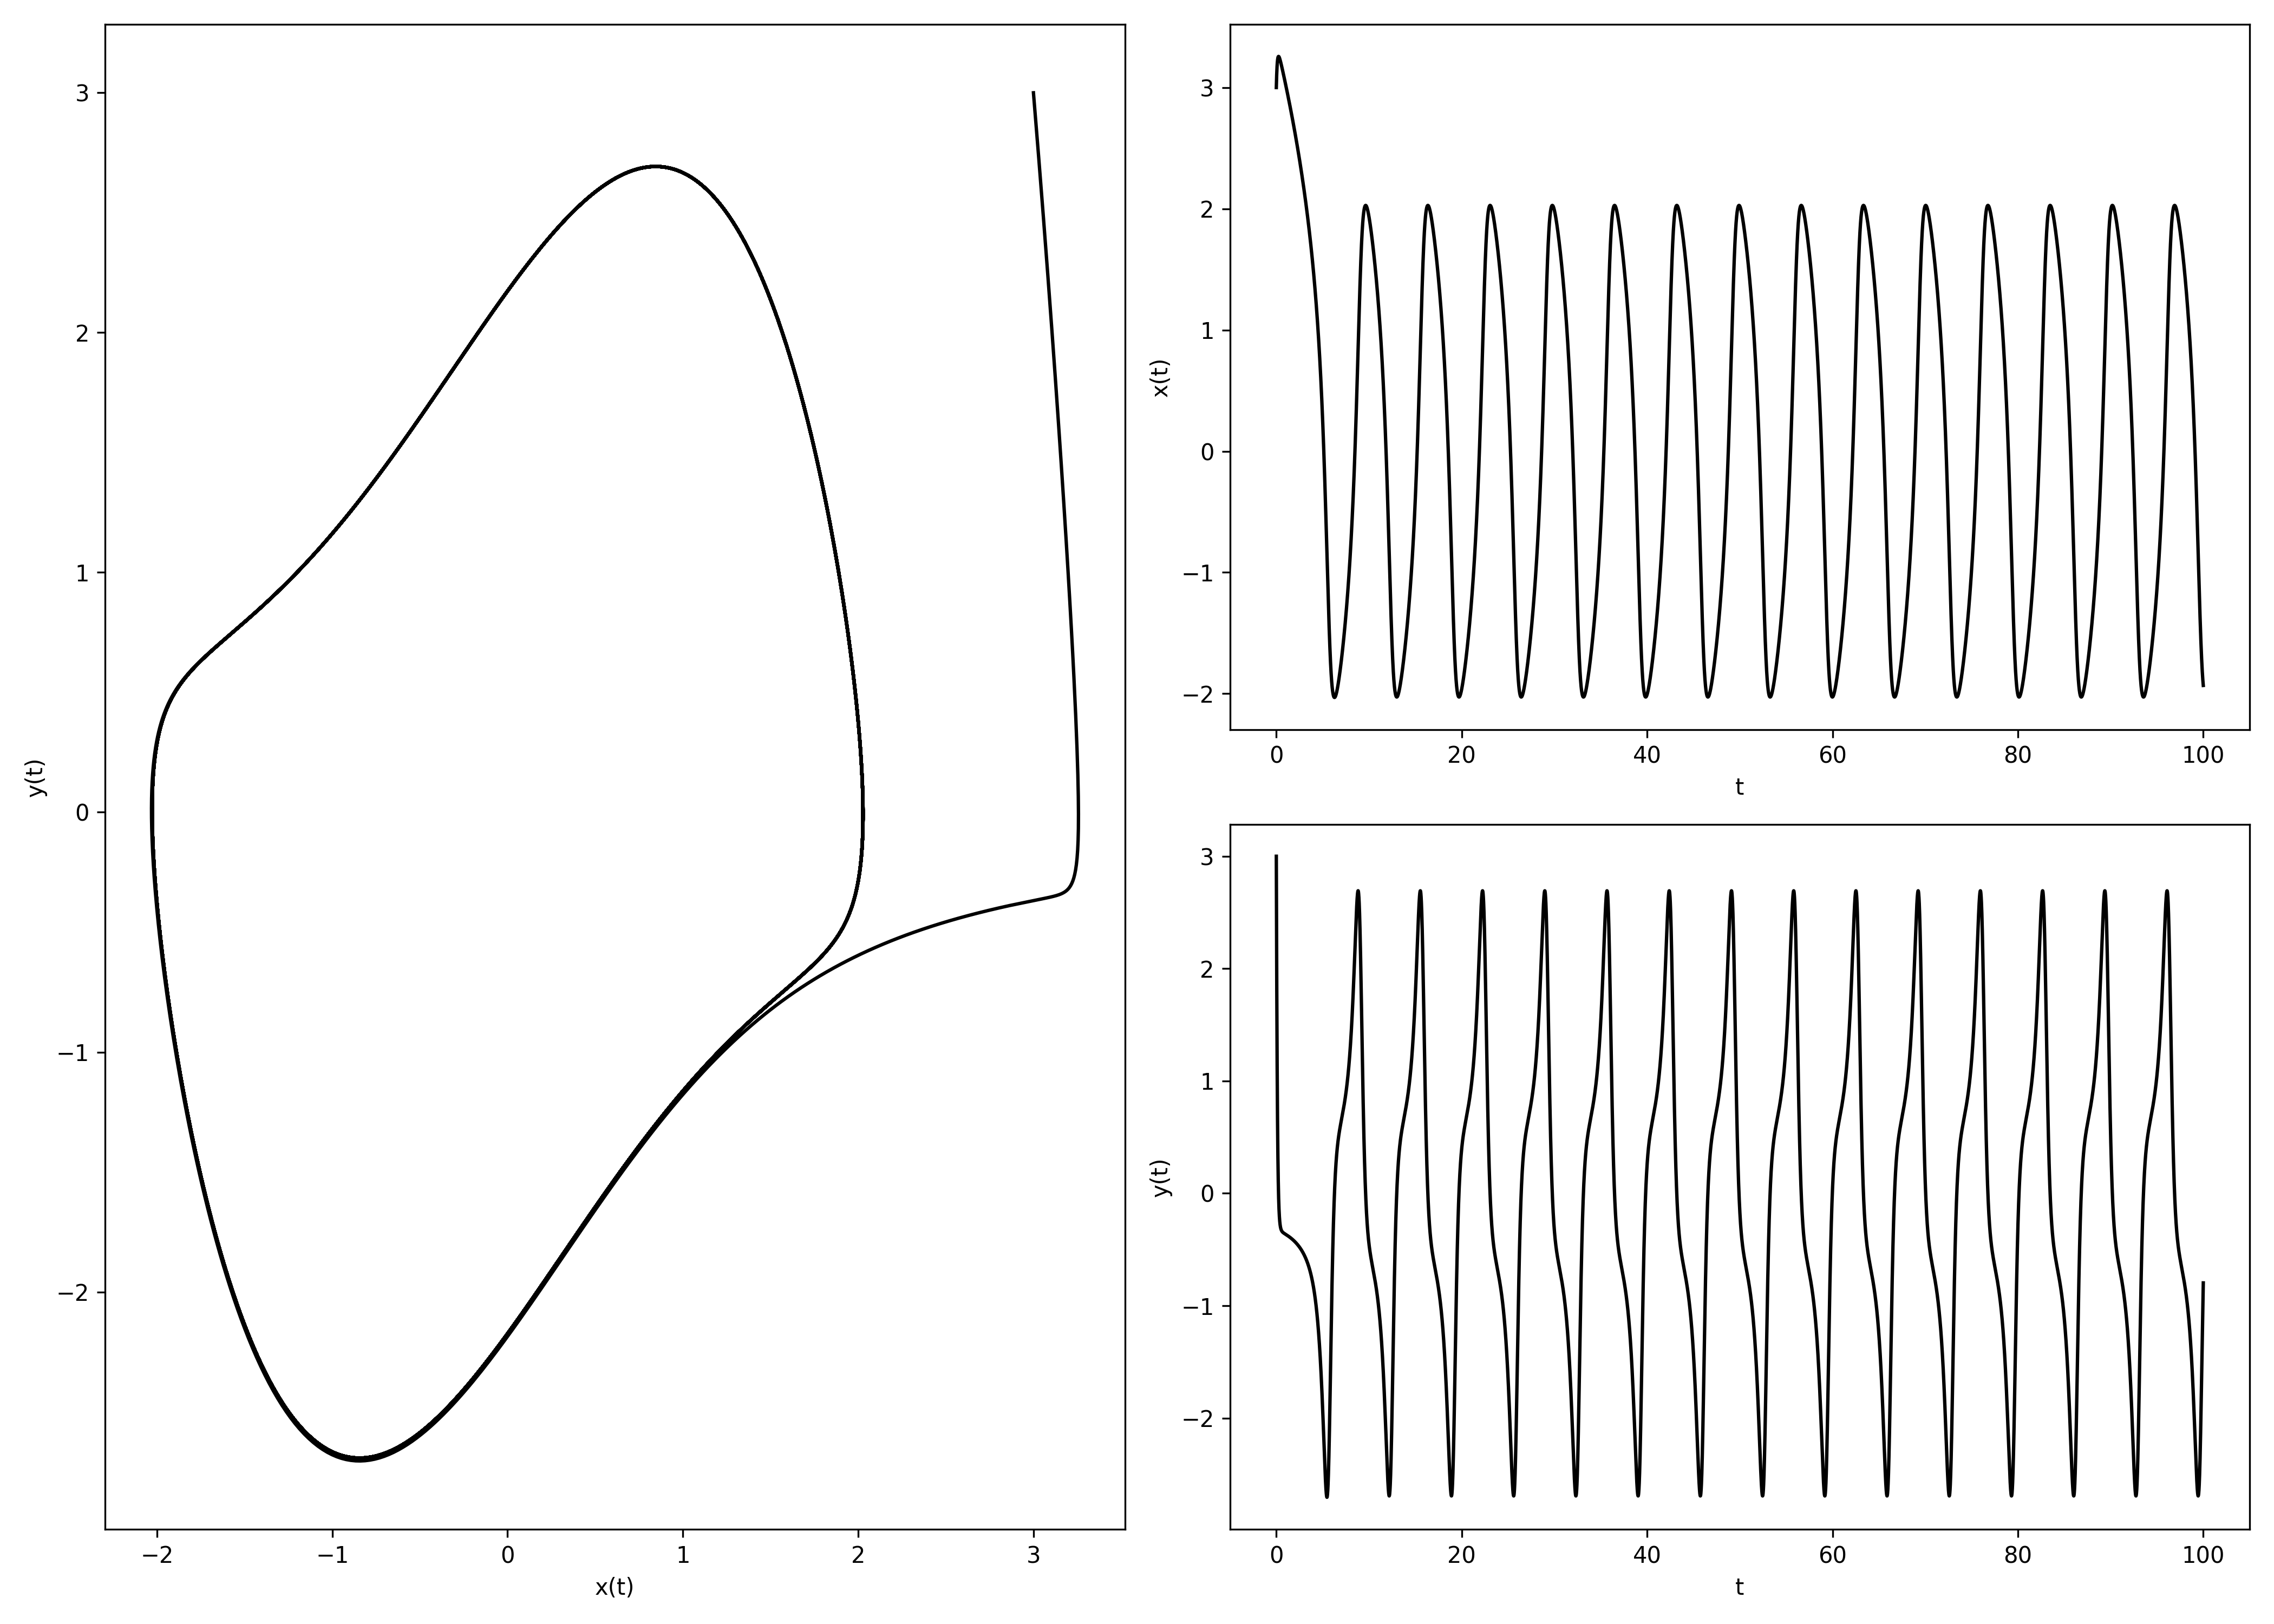
\includegraphics[scale=0.33]{x3,0y3,0mu1,0omega1,0t1,00e+02n1,00e+04.png}
\figcaption{$x_0=3.00, y_0=3.00, \mu=1,00, \omega=1.00, T = 100, N = 10000$}

\subsection{Lotka Volterra 方程式}
様々なパラメーターに対して実験結果は以下のようになった.

%N = 1000
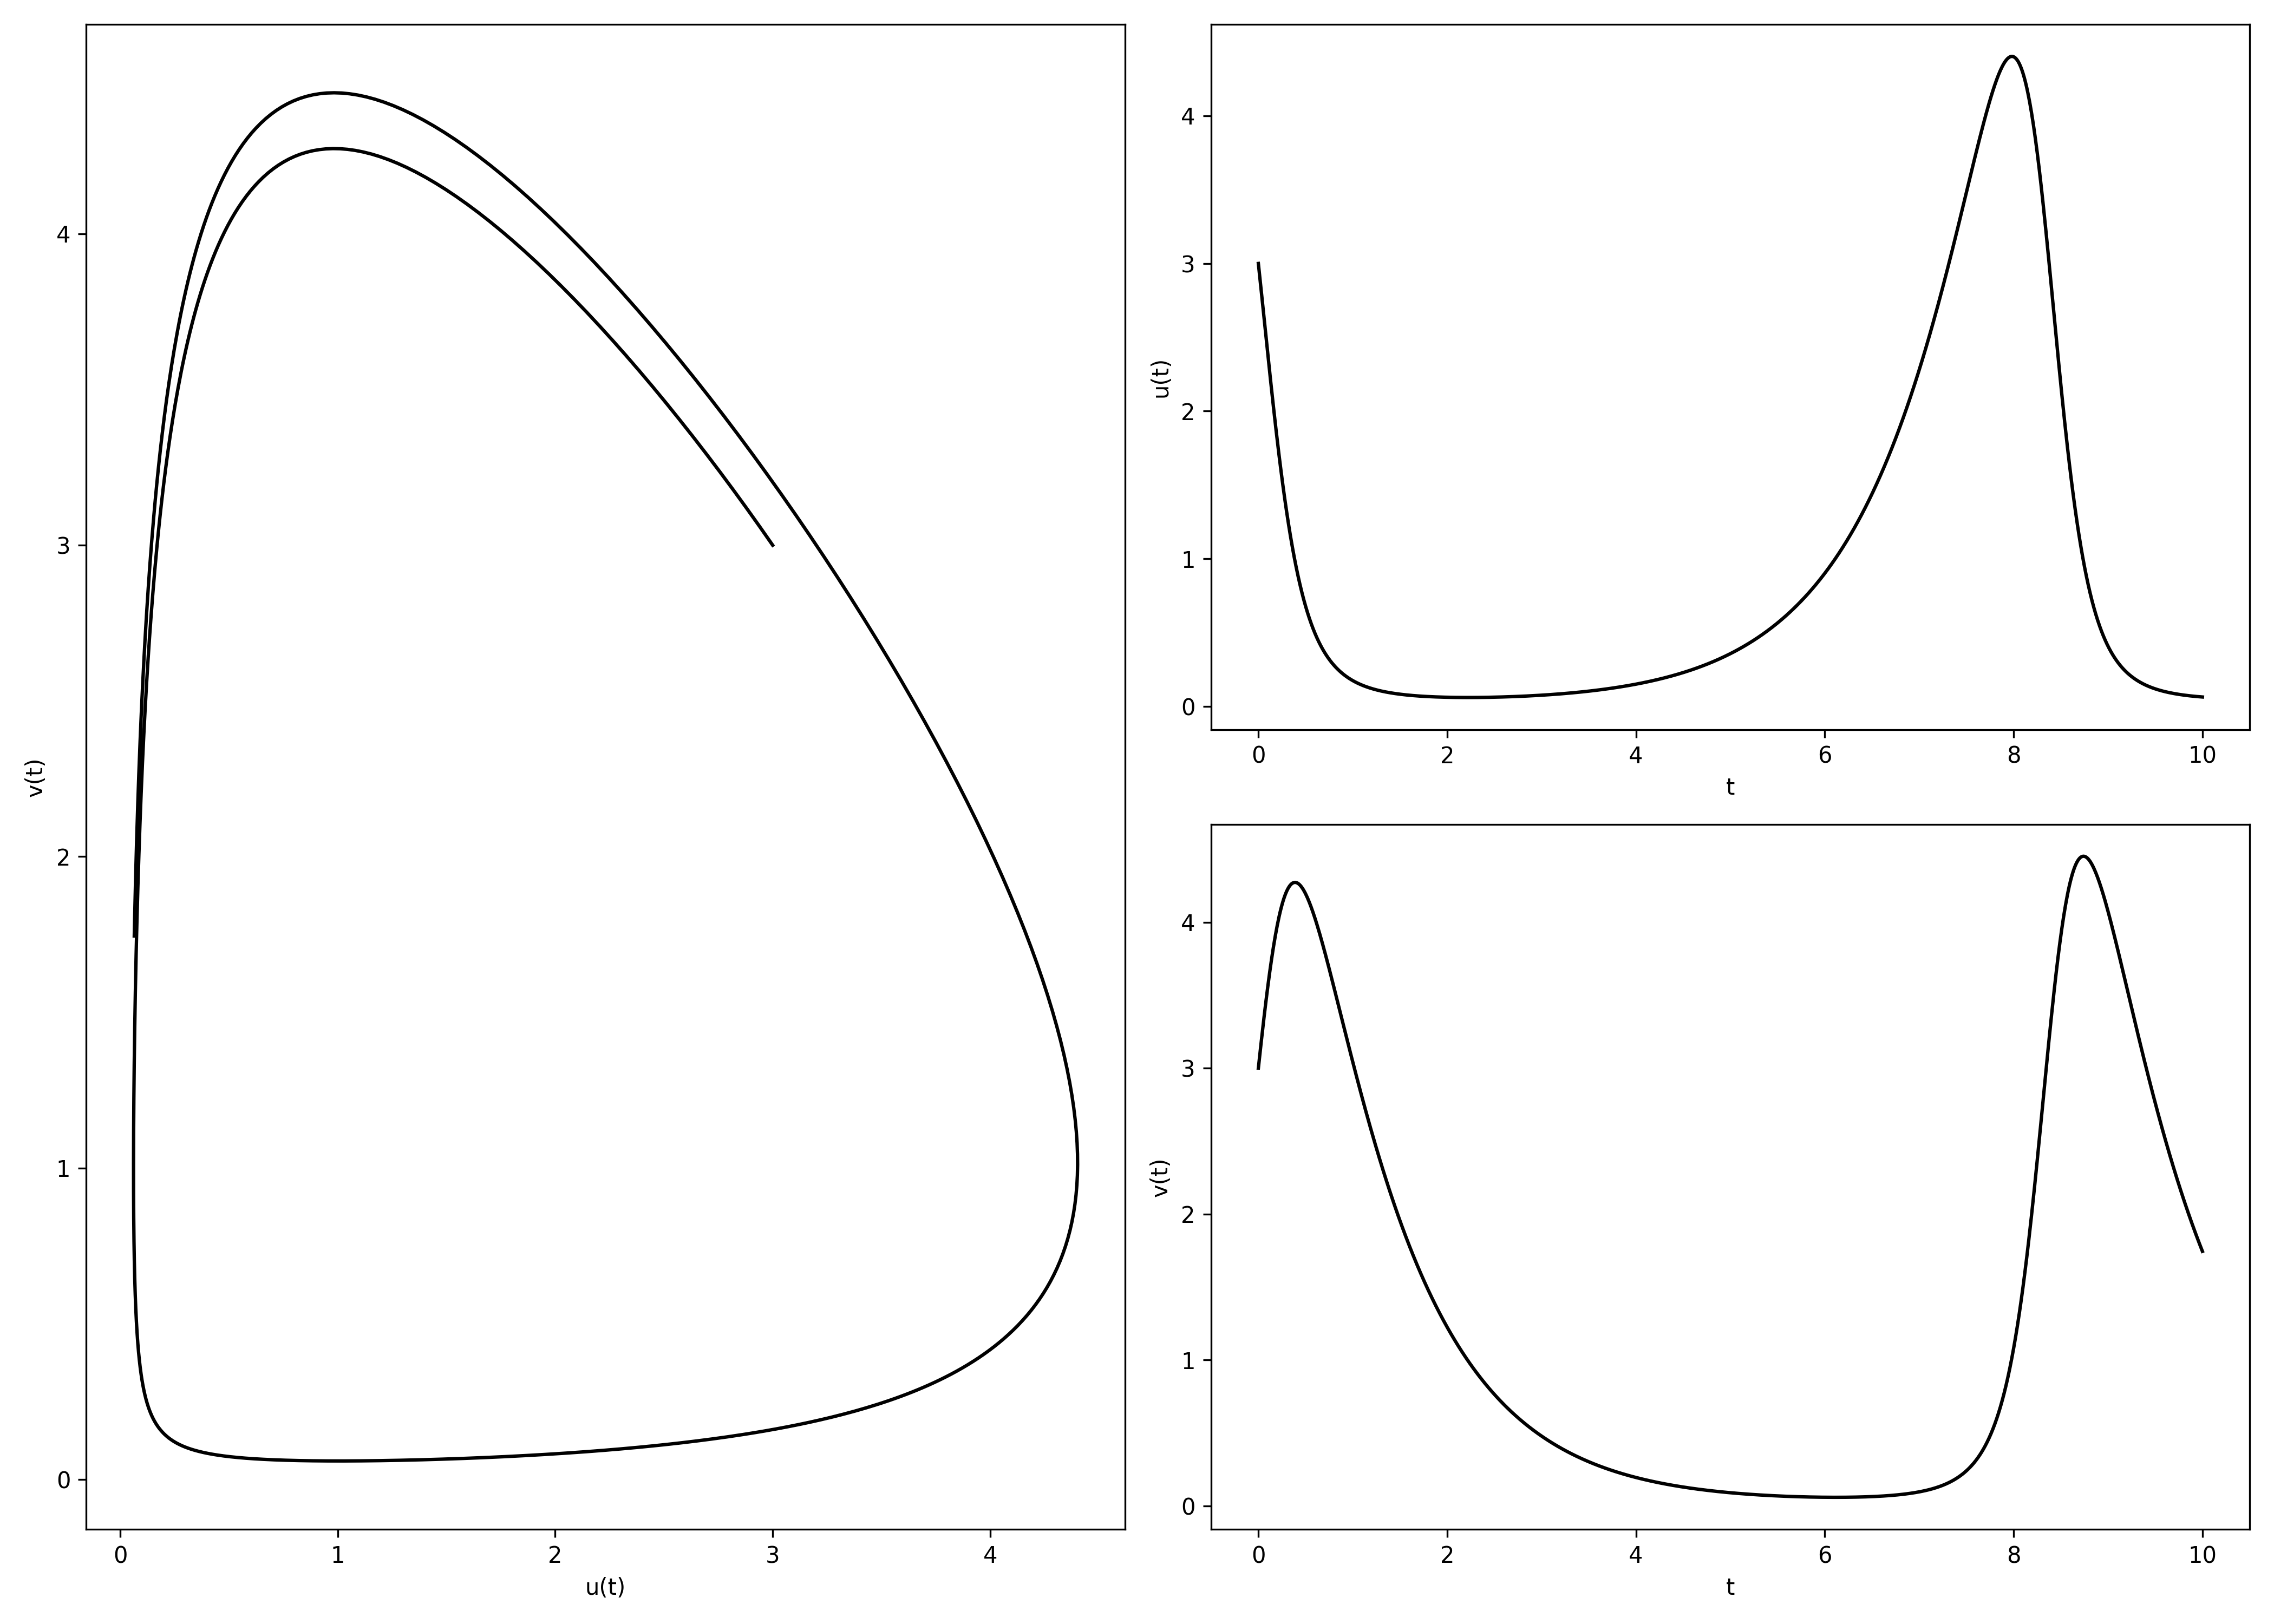
\includegraphics[scale=0.33]{u3,0v3,0a11,0b10,0c1-1,0a2-1,0b21,0c20,0t1,00e+01n1,00e+03.png}
\figcaption{$u_0=3.00, v_0=3.00, a_1=1.00, b_1=0.00, c_1=-1.00, a_2=-1.00, b_2=0.00, c_2=0.00, T = 10, N = 1000$}
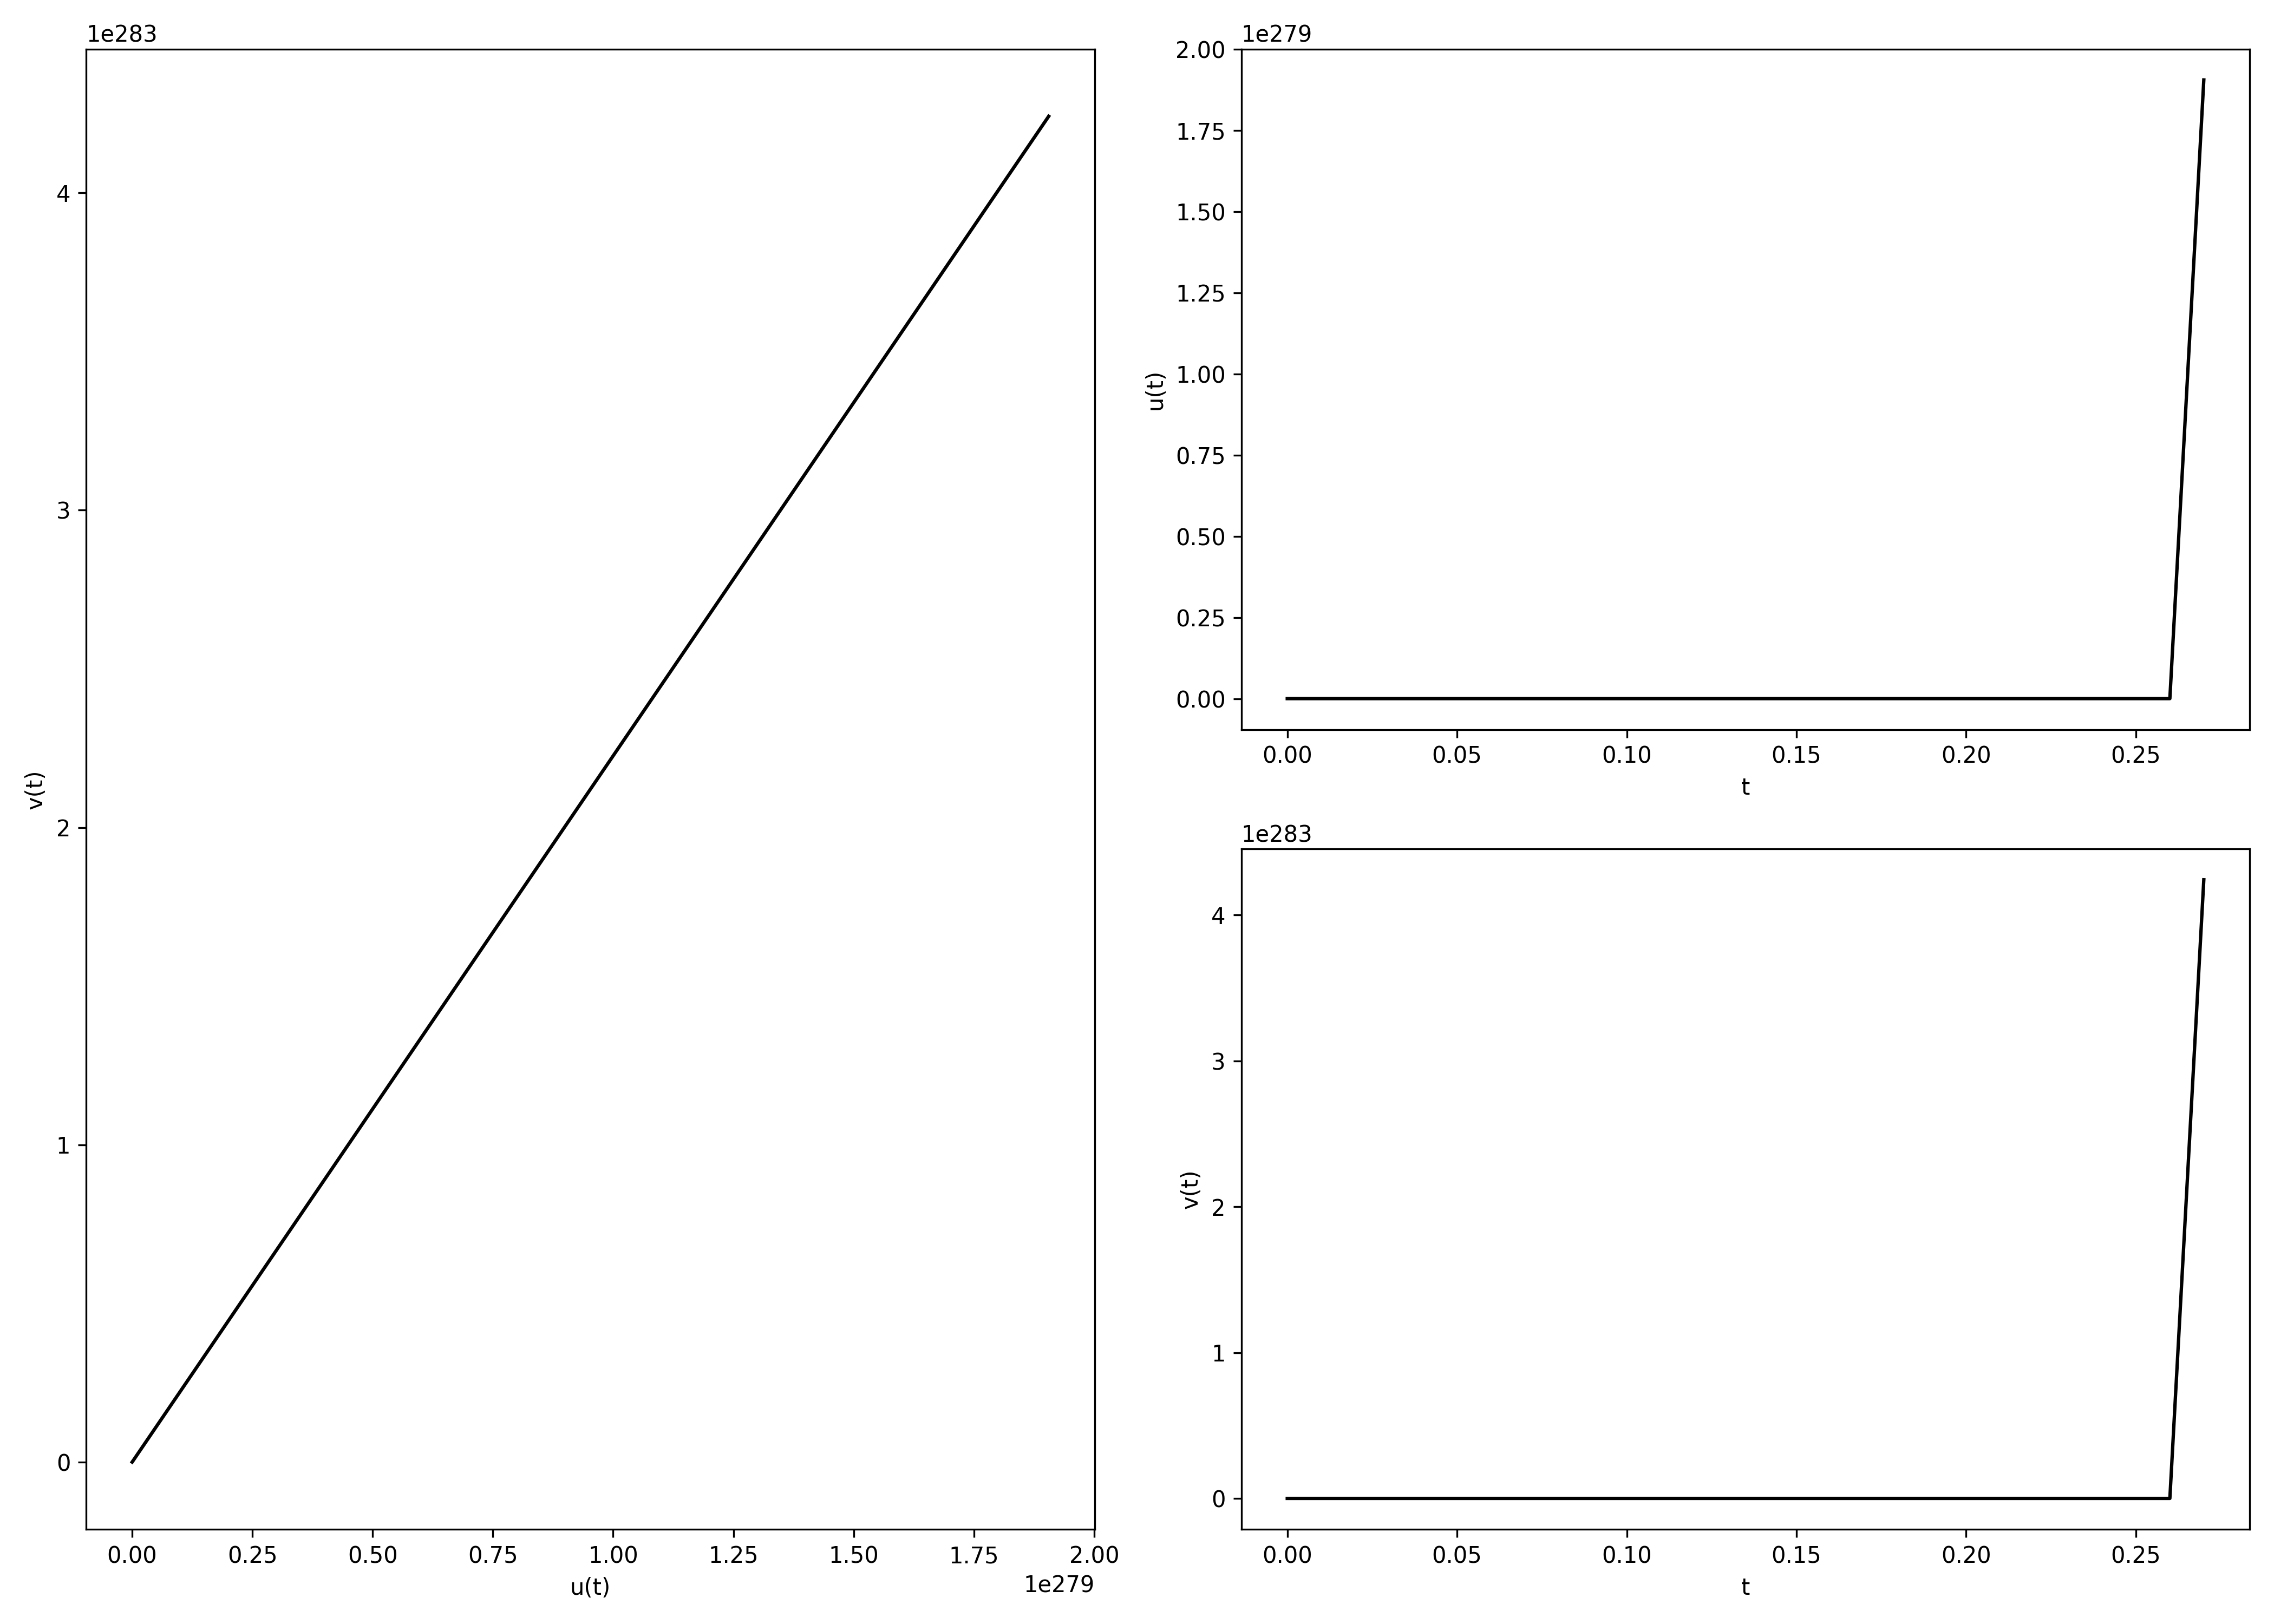
\includegraphics[scale=0.33]{u3,0v3,0a11,9b10,0c1-1,9a21,9b20,0c21,9t1,00e+01n1,00e+03.png}
\figcaption{$u_0=3.00, v_0=3.00, a_1=1.90, b_1=0.00, c_1=-1.90, a_2=1.90, b_2=0.00, c_2=1.90, T = 10, N = 1000$}
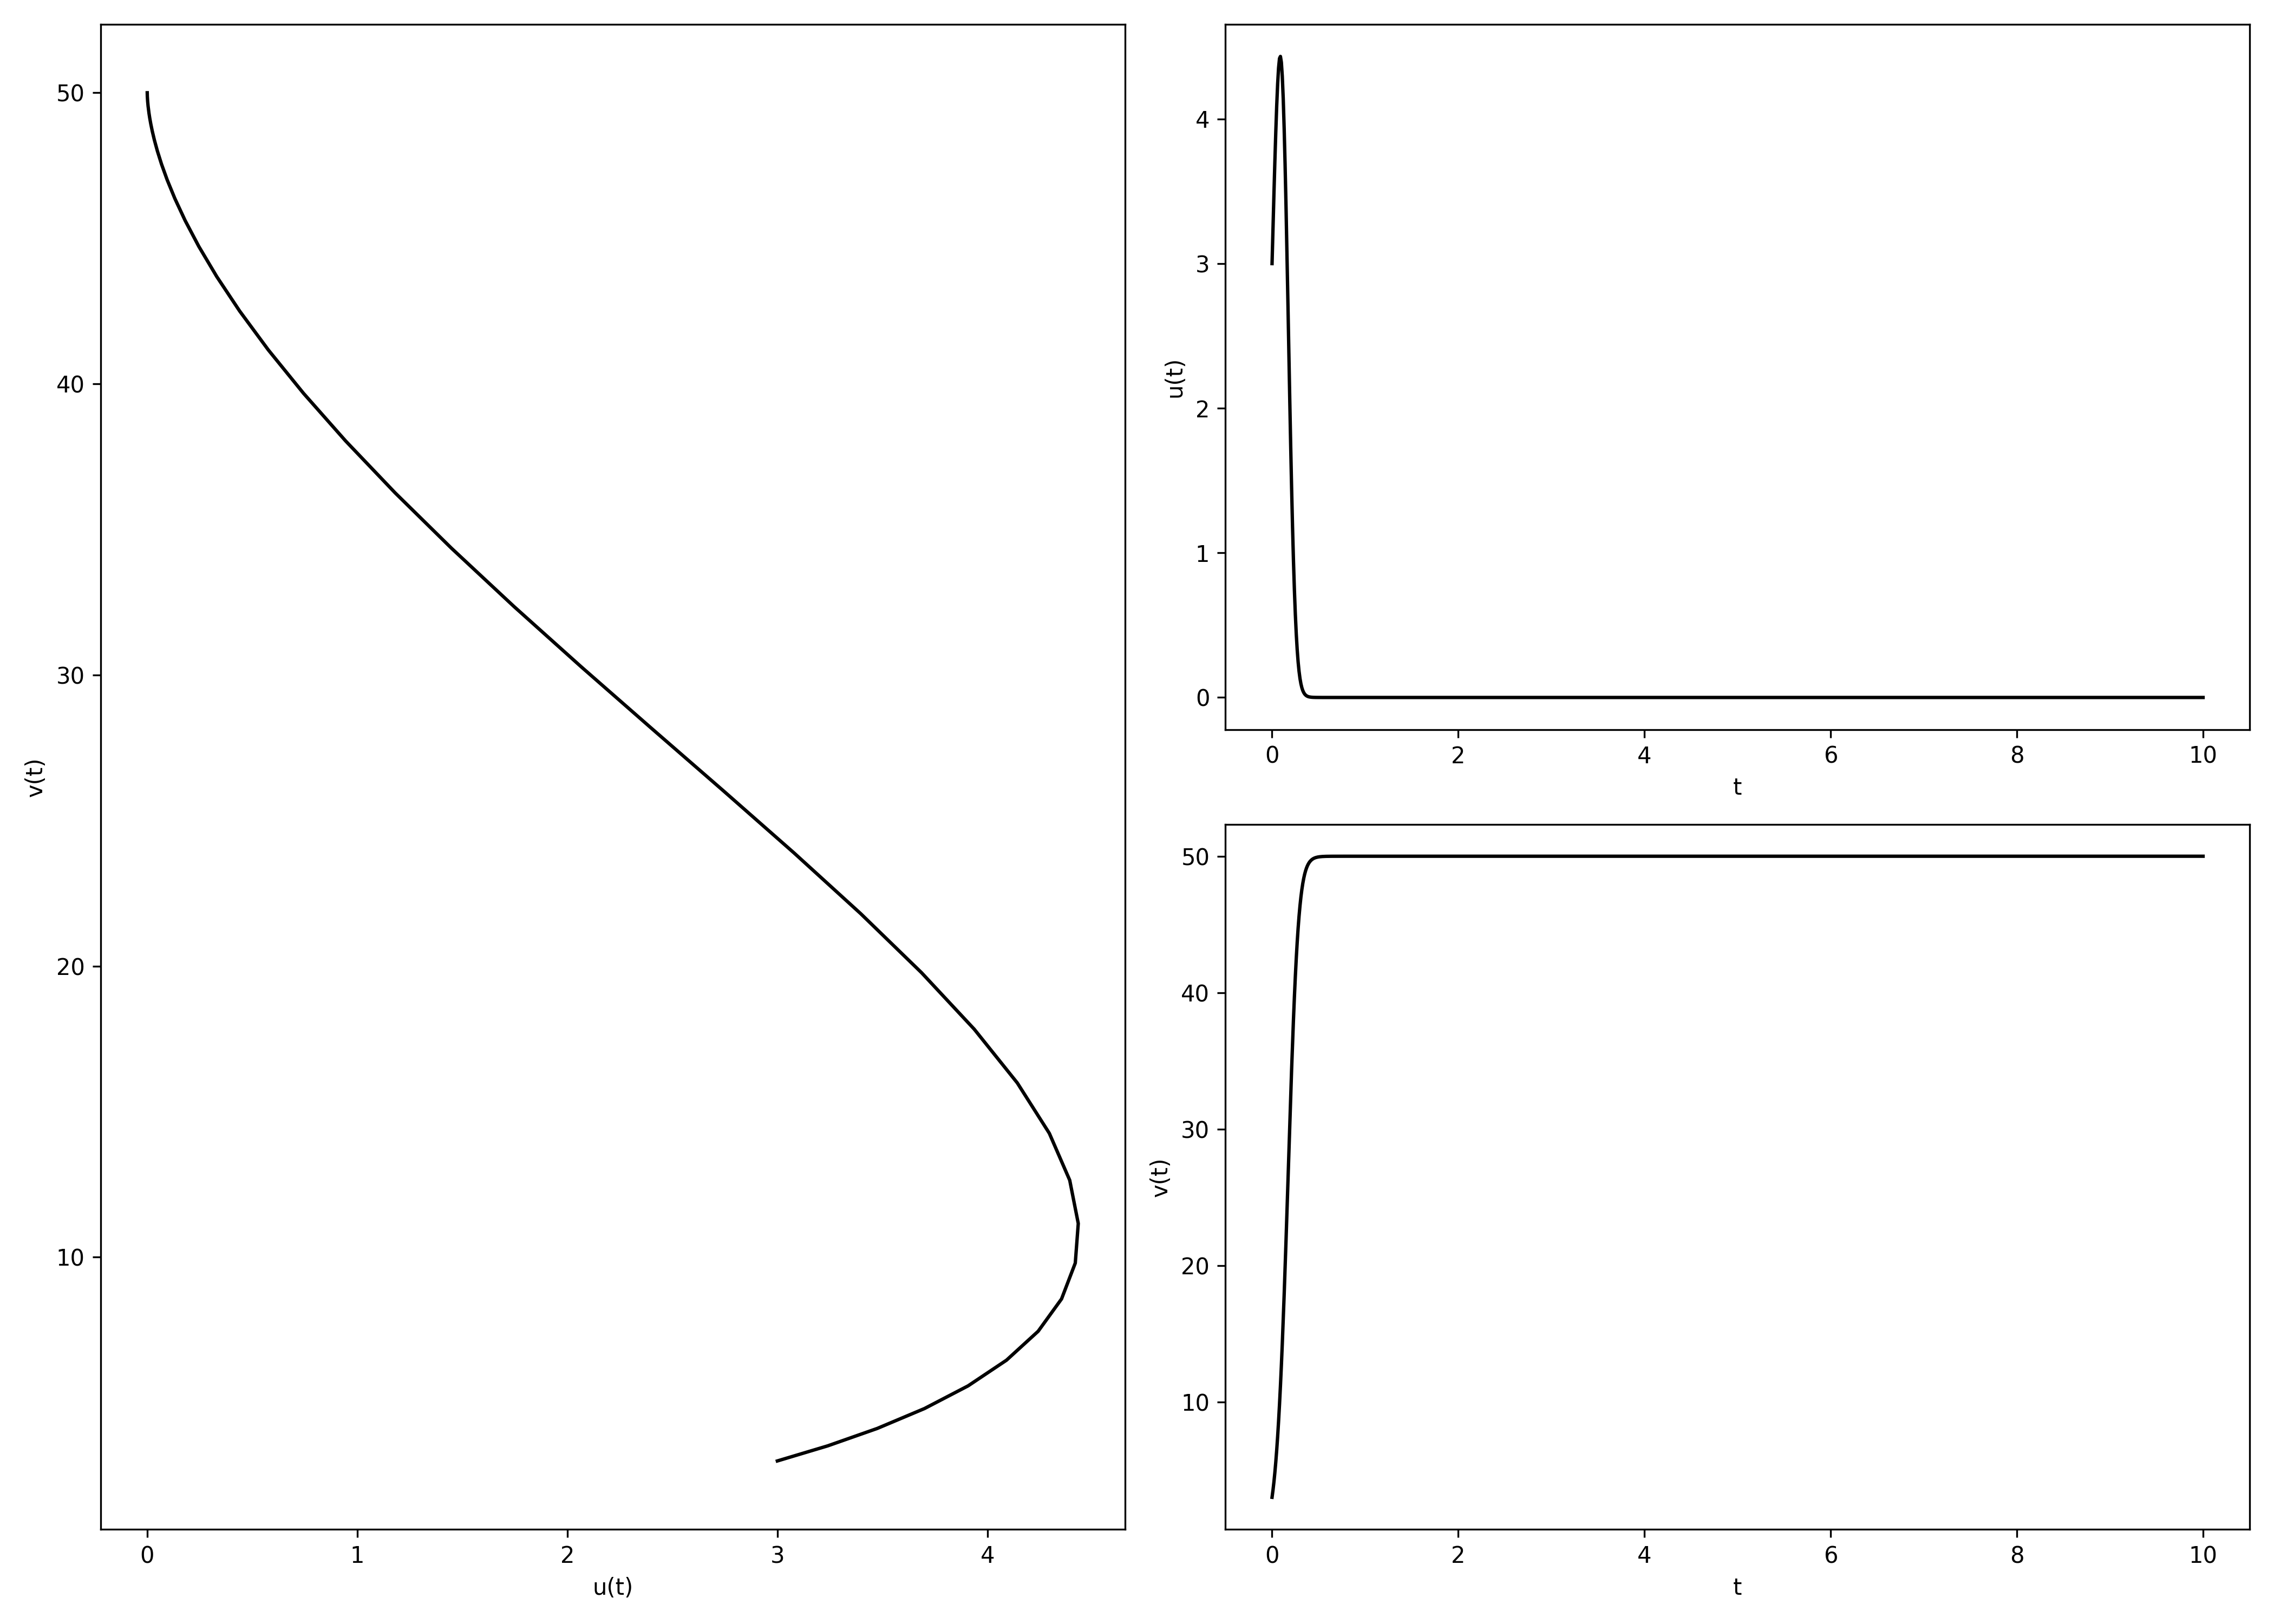
\includegraphics[scale=0.33]{u3,0v3,0a114,0b1-1,1c1-0,9a220,0b2-0,5c2-0,4t1,00e+01n1,00e+03.png}
\figcaption{$u_0=3.00, v_0=3.00, a_1=14.00, b_1=-1.10, c_1=-0.90, a_2=20.00, b_2=-0.50, c_2-=0.40, T = 10, N = 1000$}
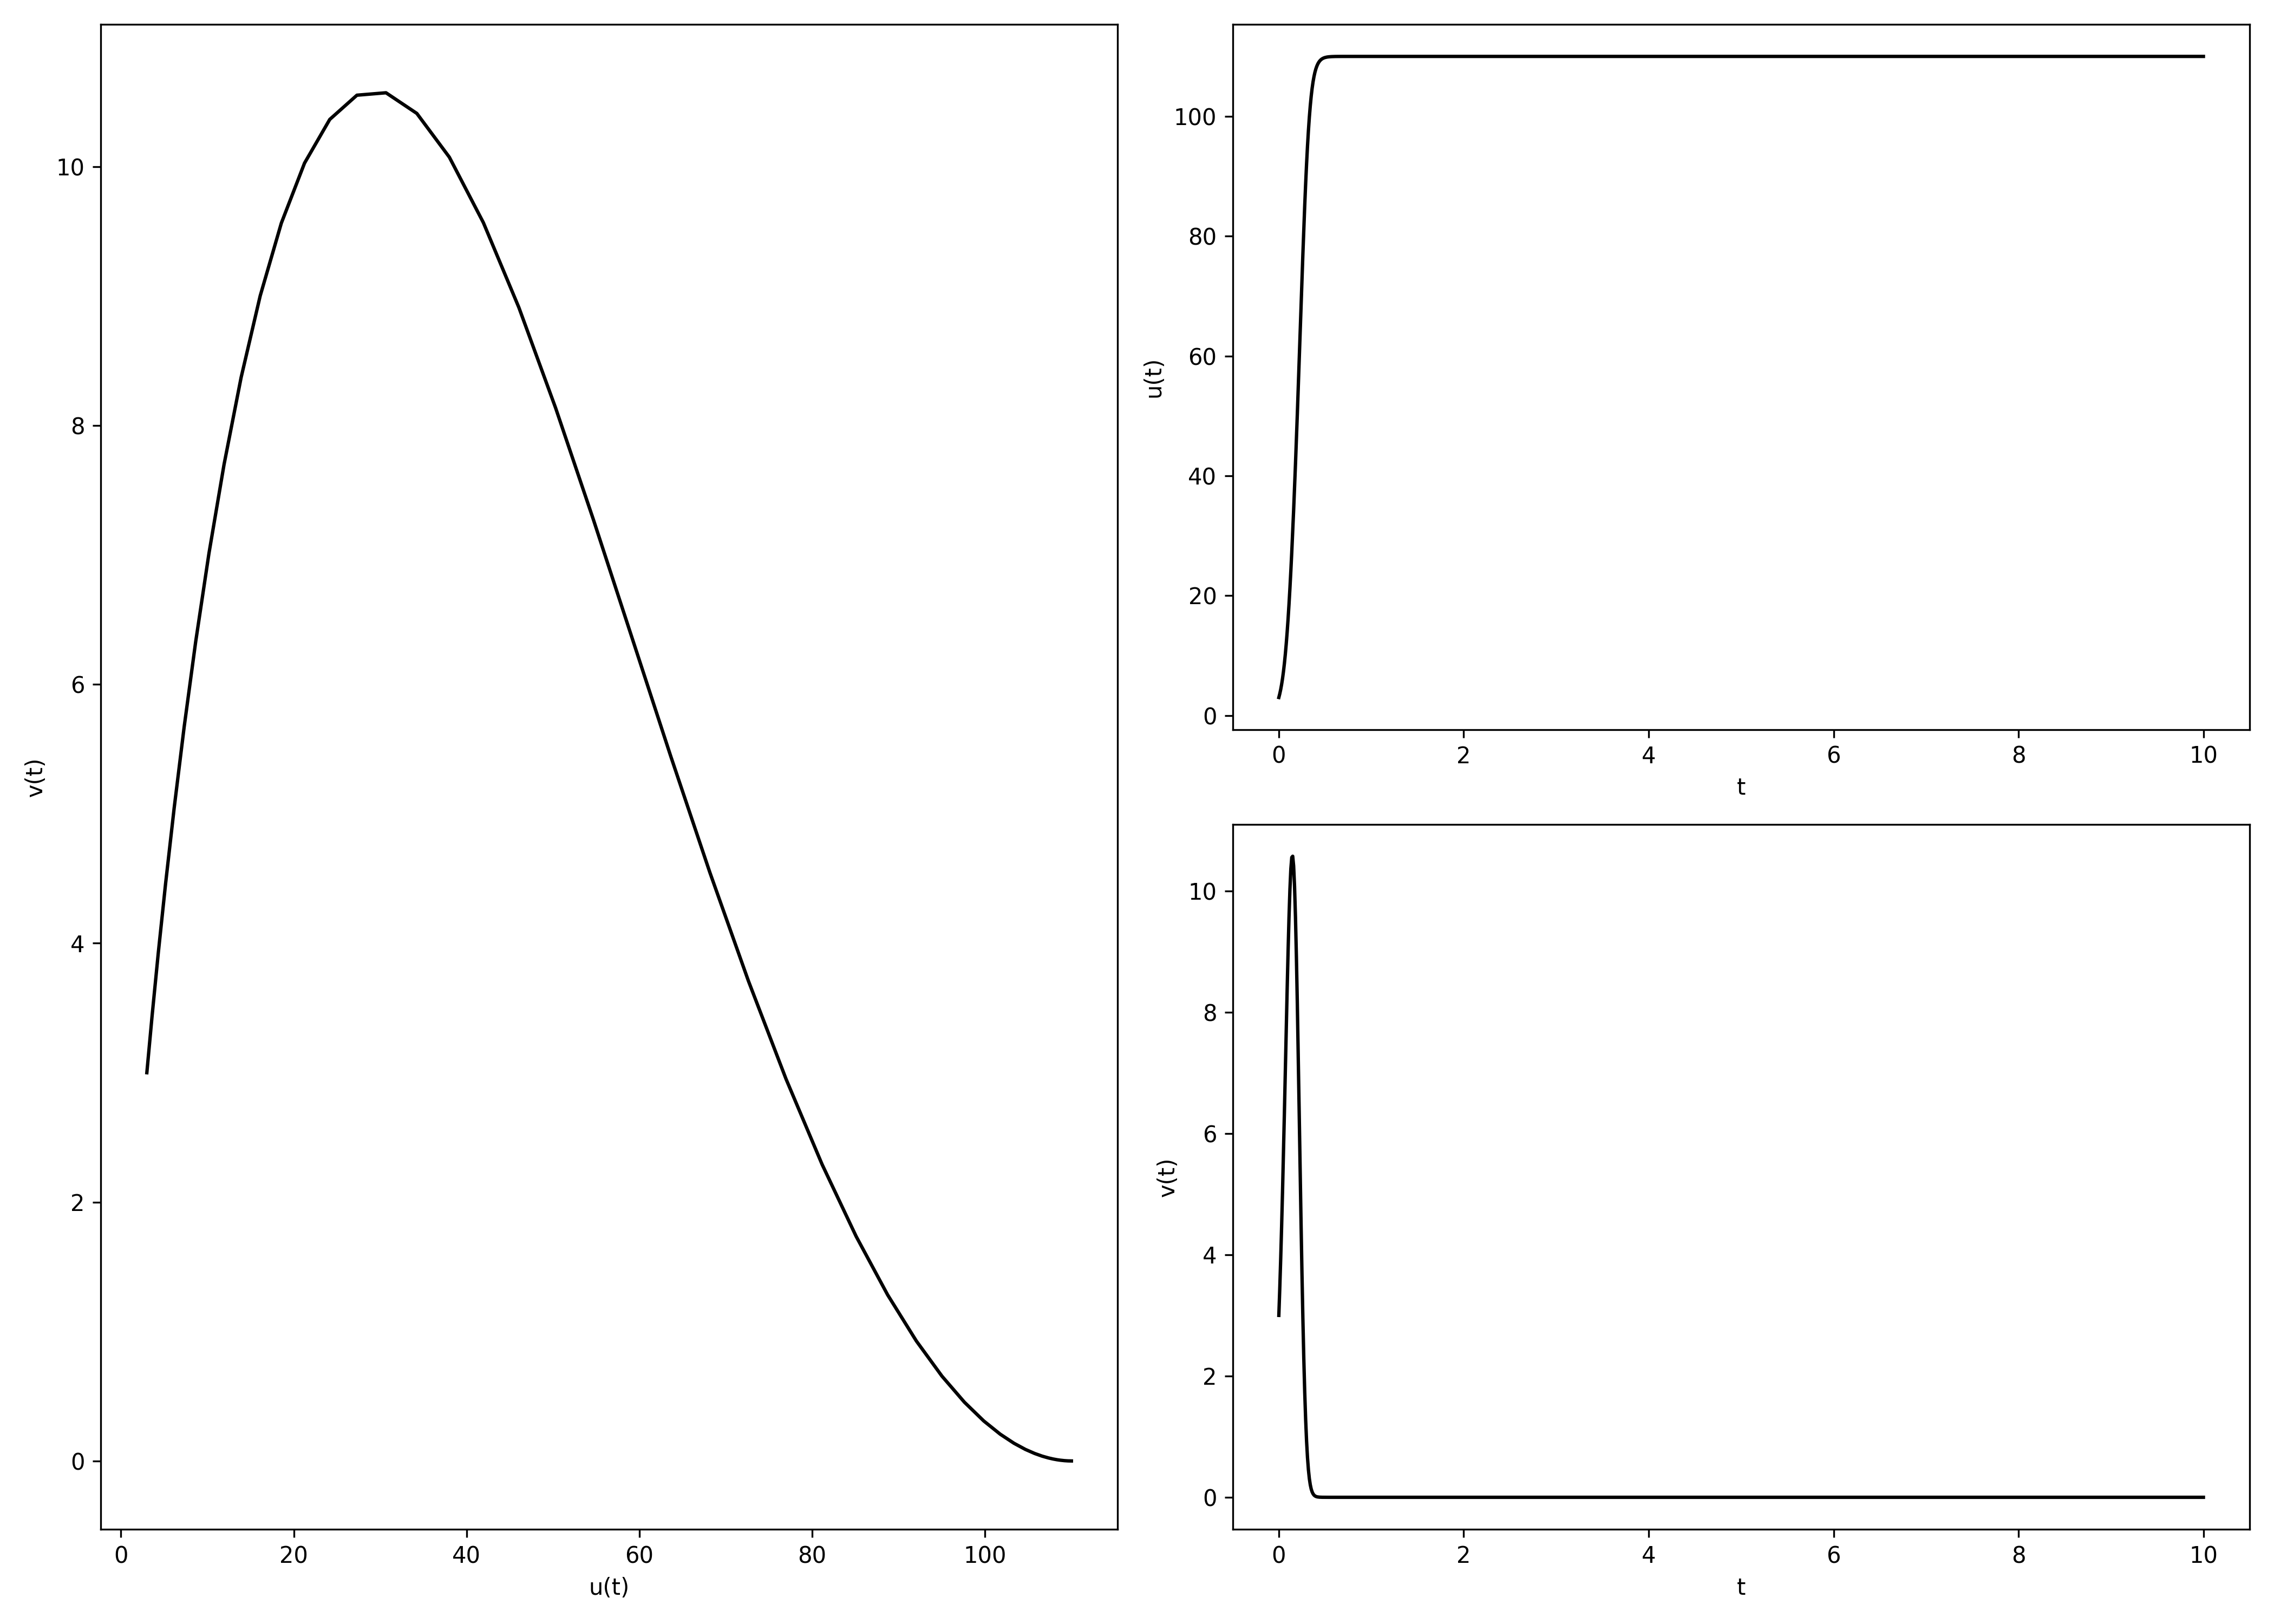
\includegraphics[scale=0.33]{u3,0v3,0a122,0b1-0,2c1-0,4a217,0b2-0,5c2-0,3t1,00e+01n1,00e+03.png}
\figcaption{$u_0=3.00, v_0=3.00, a_1=22.00, b_1=-0.20, c_1=-0.40, a_2=17.00, b_2=-0.50, c_2=-0.30, T = 10, N = 1000$}
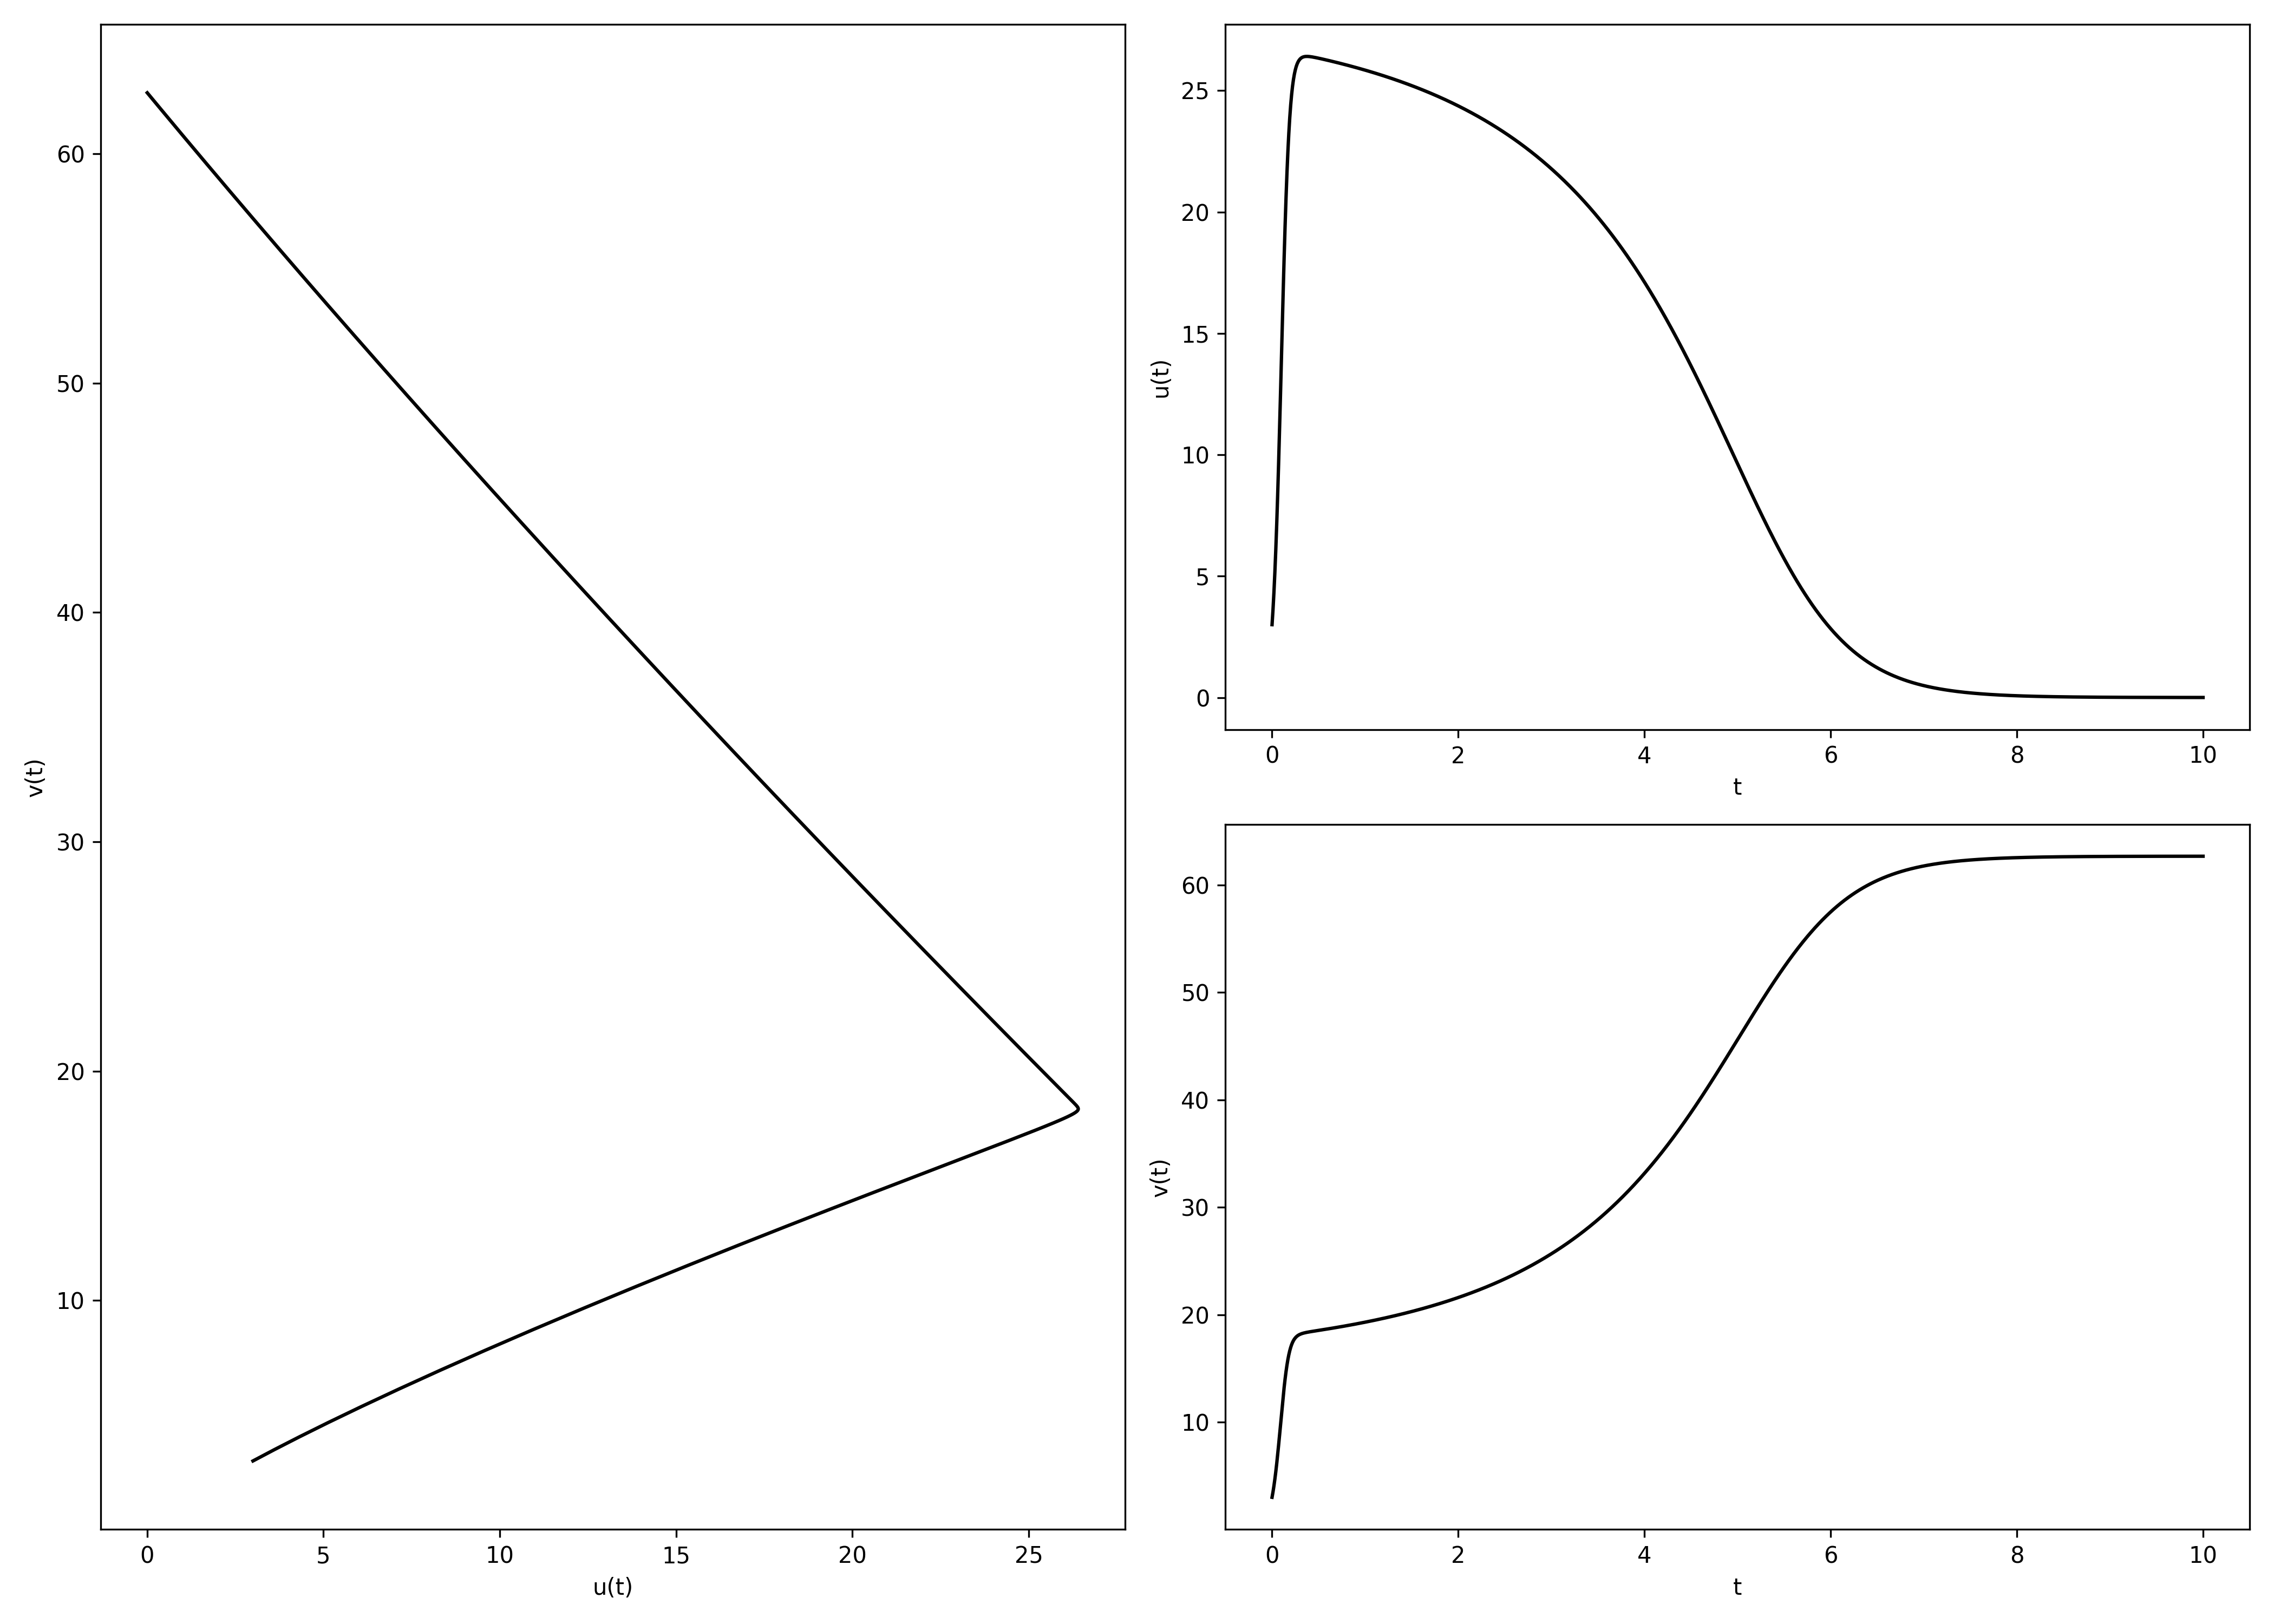
\includegraphics[scale=0.33]{u3,0v3,0a123,2b1-0,6c1-0,4a218,8b2-0,5c2-0,3t1,00e+01n1,00e+03.png}
\figcaption{$u_0=3.00, v_0=3.00, a_1=23.20, b_1=-0.60, c_1=-0.40, a_2=18.80, b_2=-0.50, c_2=-0.30, T = 10, N = 1000$}
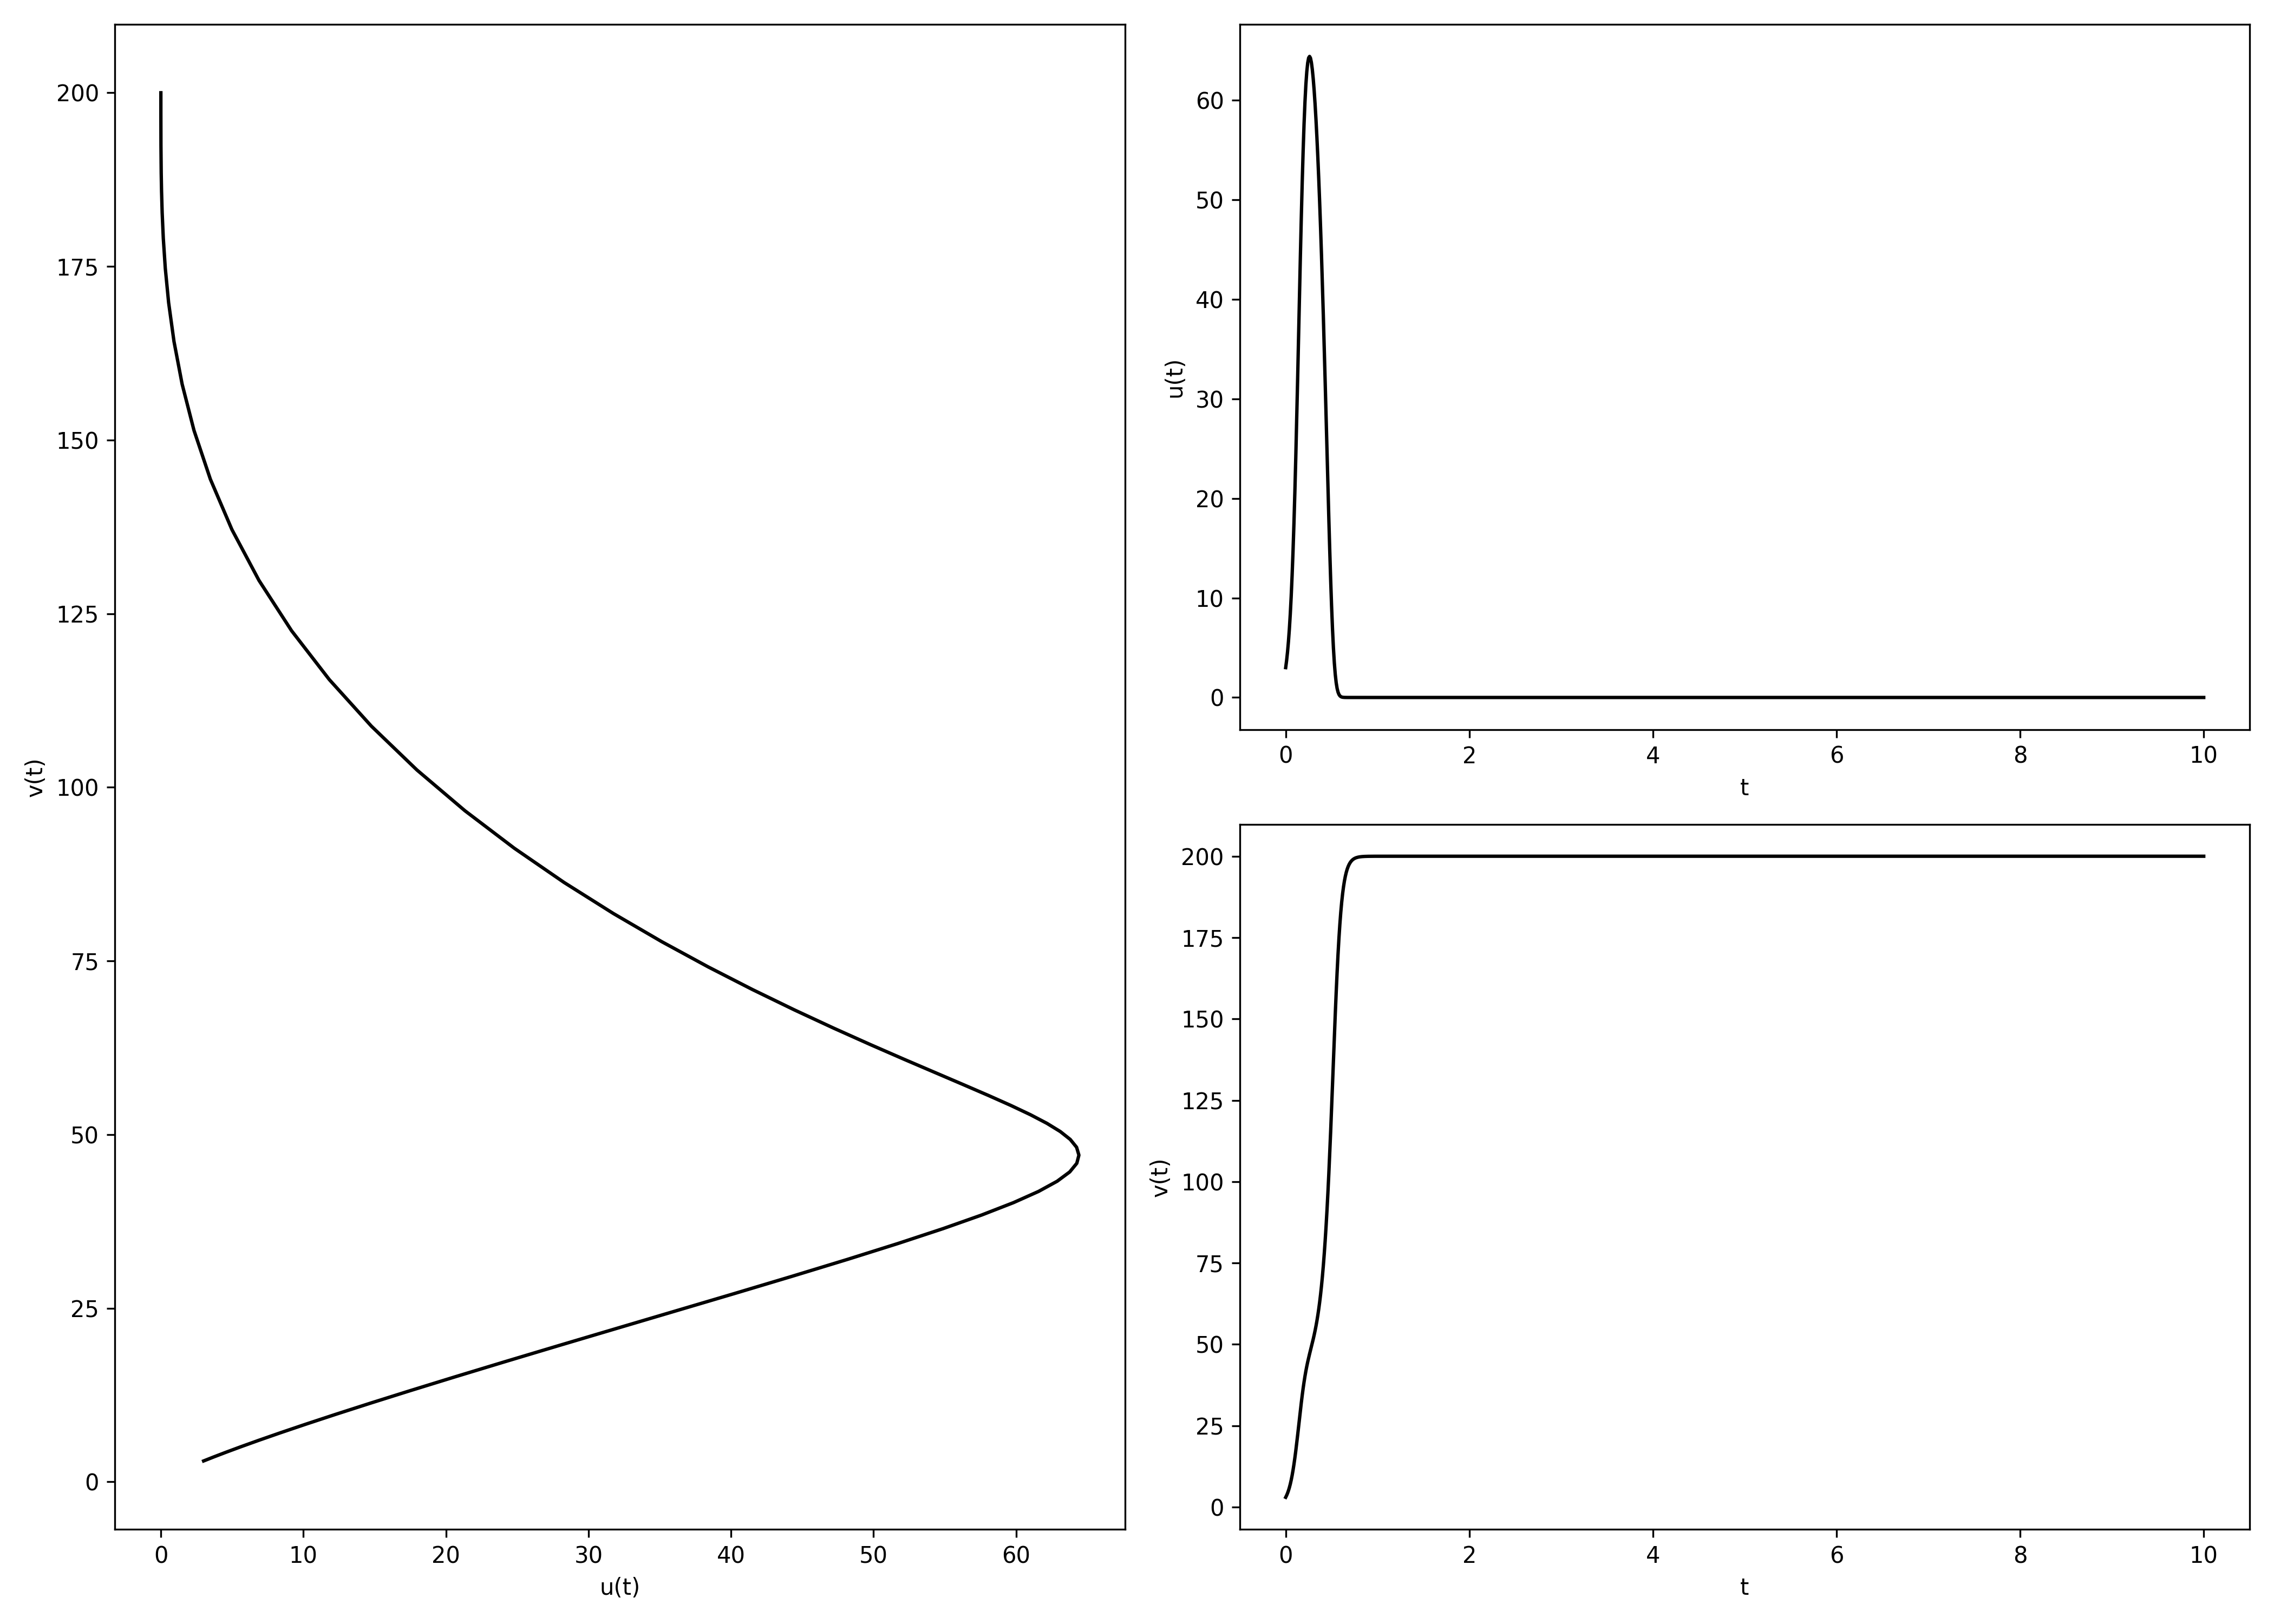
\includegraphics[scale=0.33]{u3,0v3,0a125,0b1-0,1c1-0,4a220,0b2-0,2c2-0,1t1,00e+01n1,00e+03.png}
\figcaption{$u_0=3.00, v_0=3.00, a_1=25.00, b_1=-0.10, c_1=-0.40, a_2=20.00, b_2=-0.20, c_2=-0.10, T = 10, N = 1000$}
%N = 2000
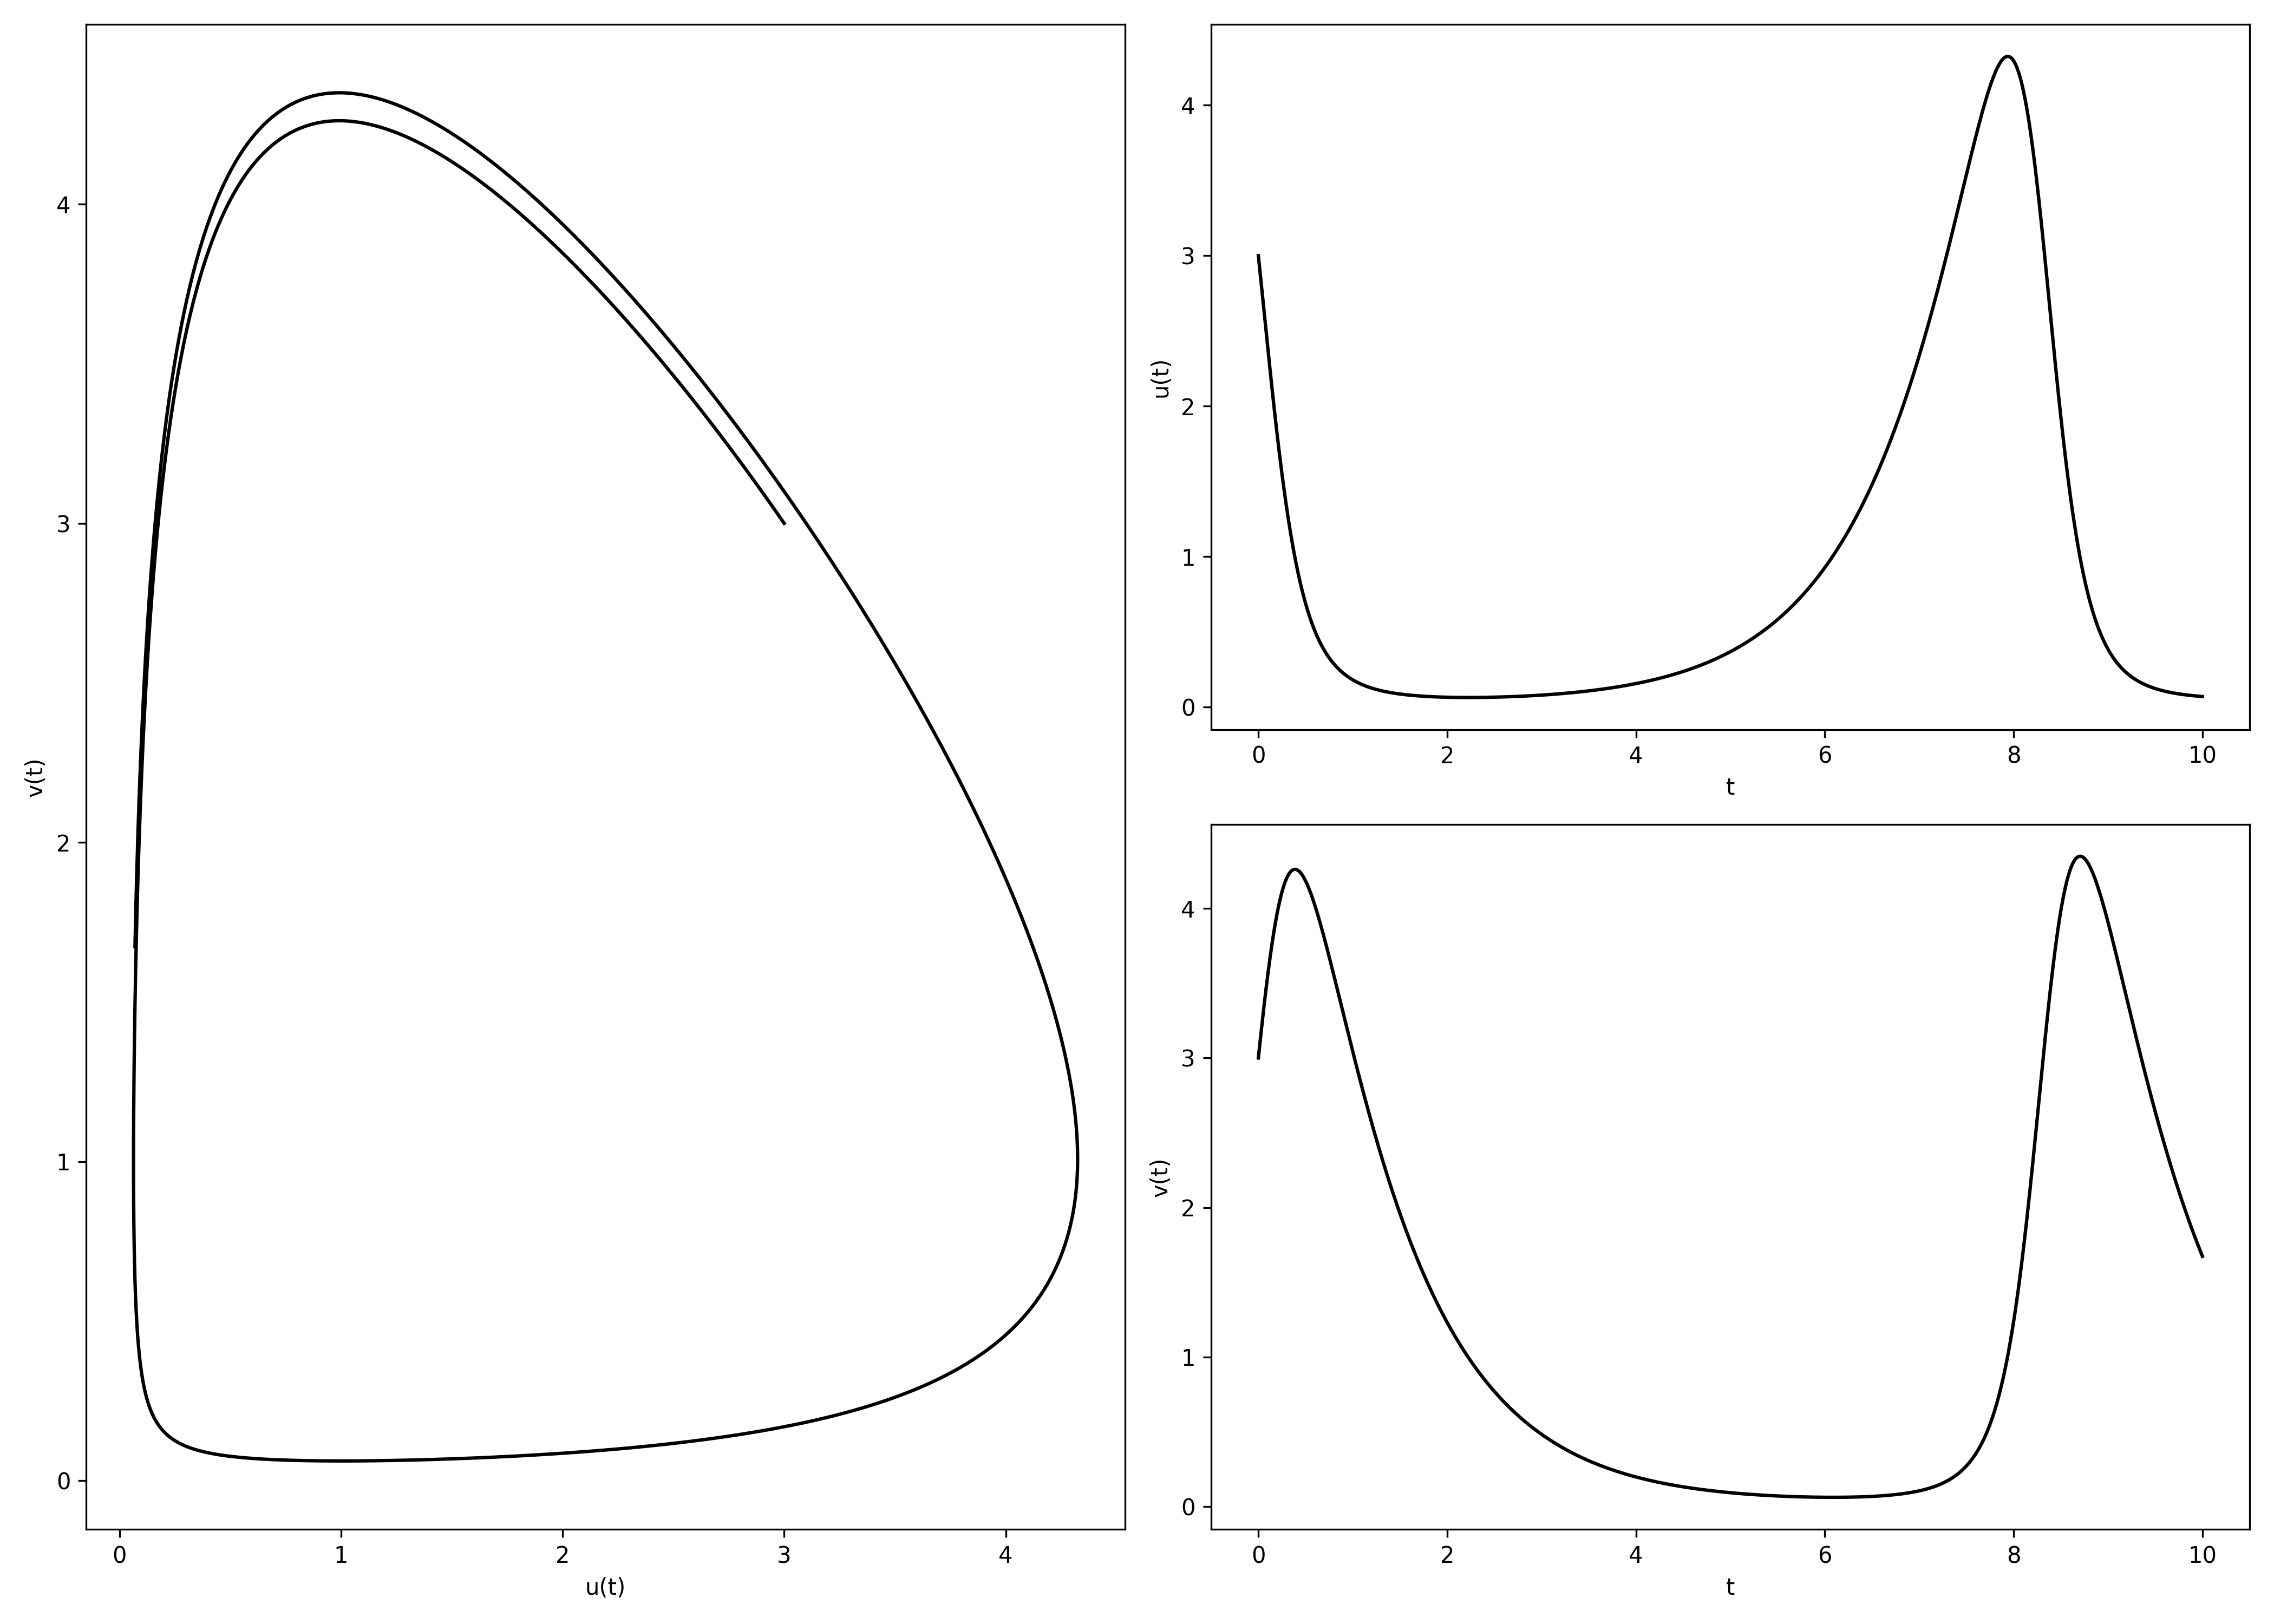
\includegraphics[scale=0.33]{u3,0v3,0a11,0b10,0c1-1,0a2-1,0b21,0c20,0t1,00e+01n2,00e+03.png}
\figcaption{$u_0=3.00, v_0=3.00, a_1=1.00, b_1=0.00, c_1=-1.00, a_2=-1.00, b_2=0.00, c_2=0.00, T = 10, N = 2000$}
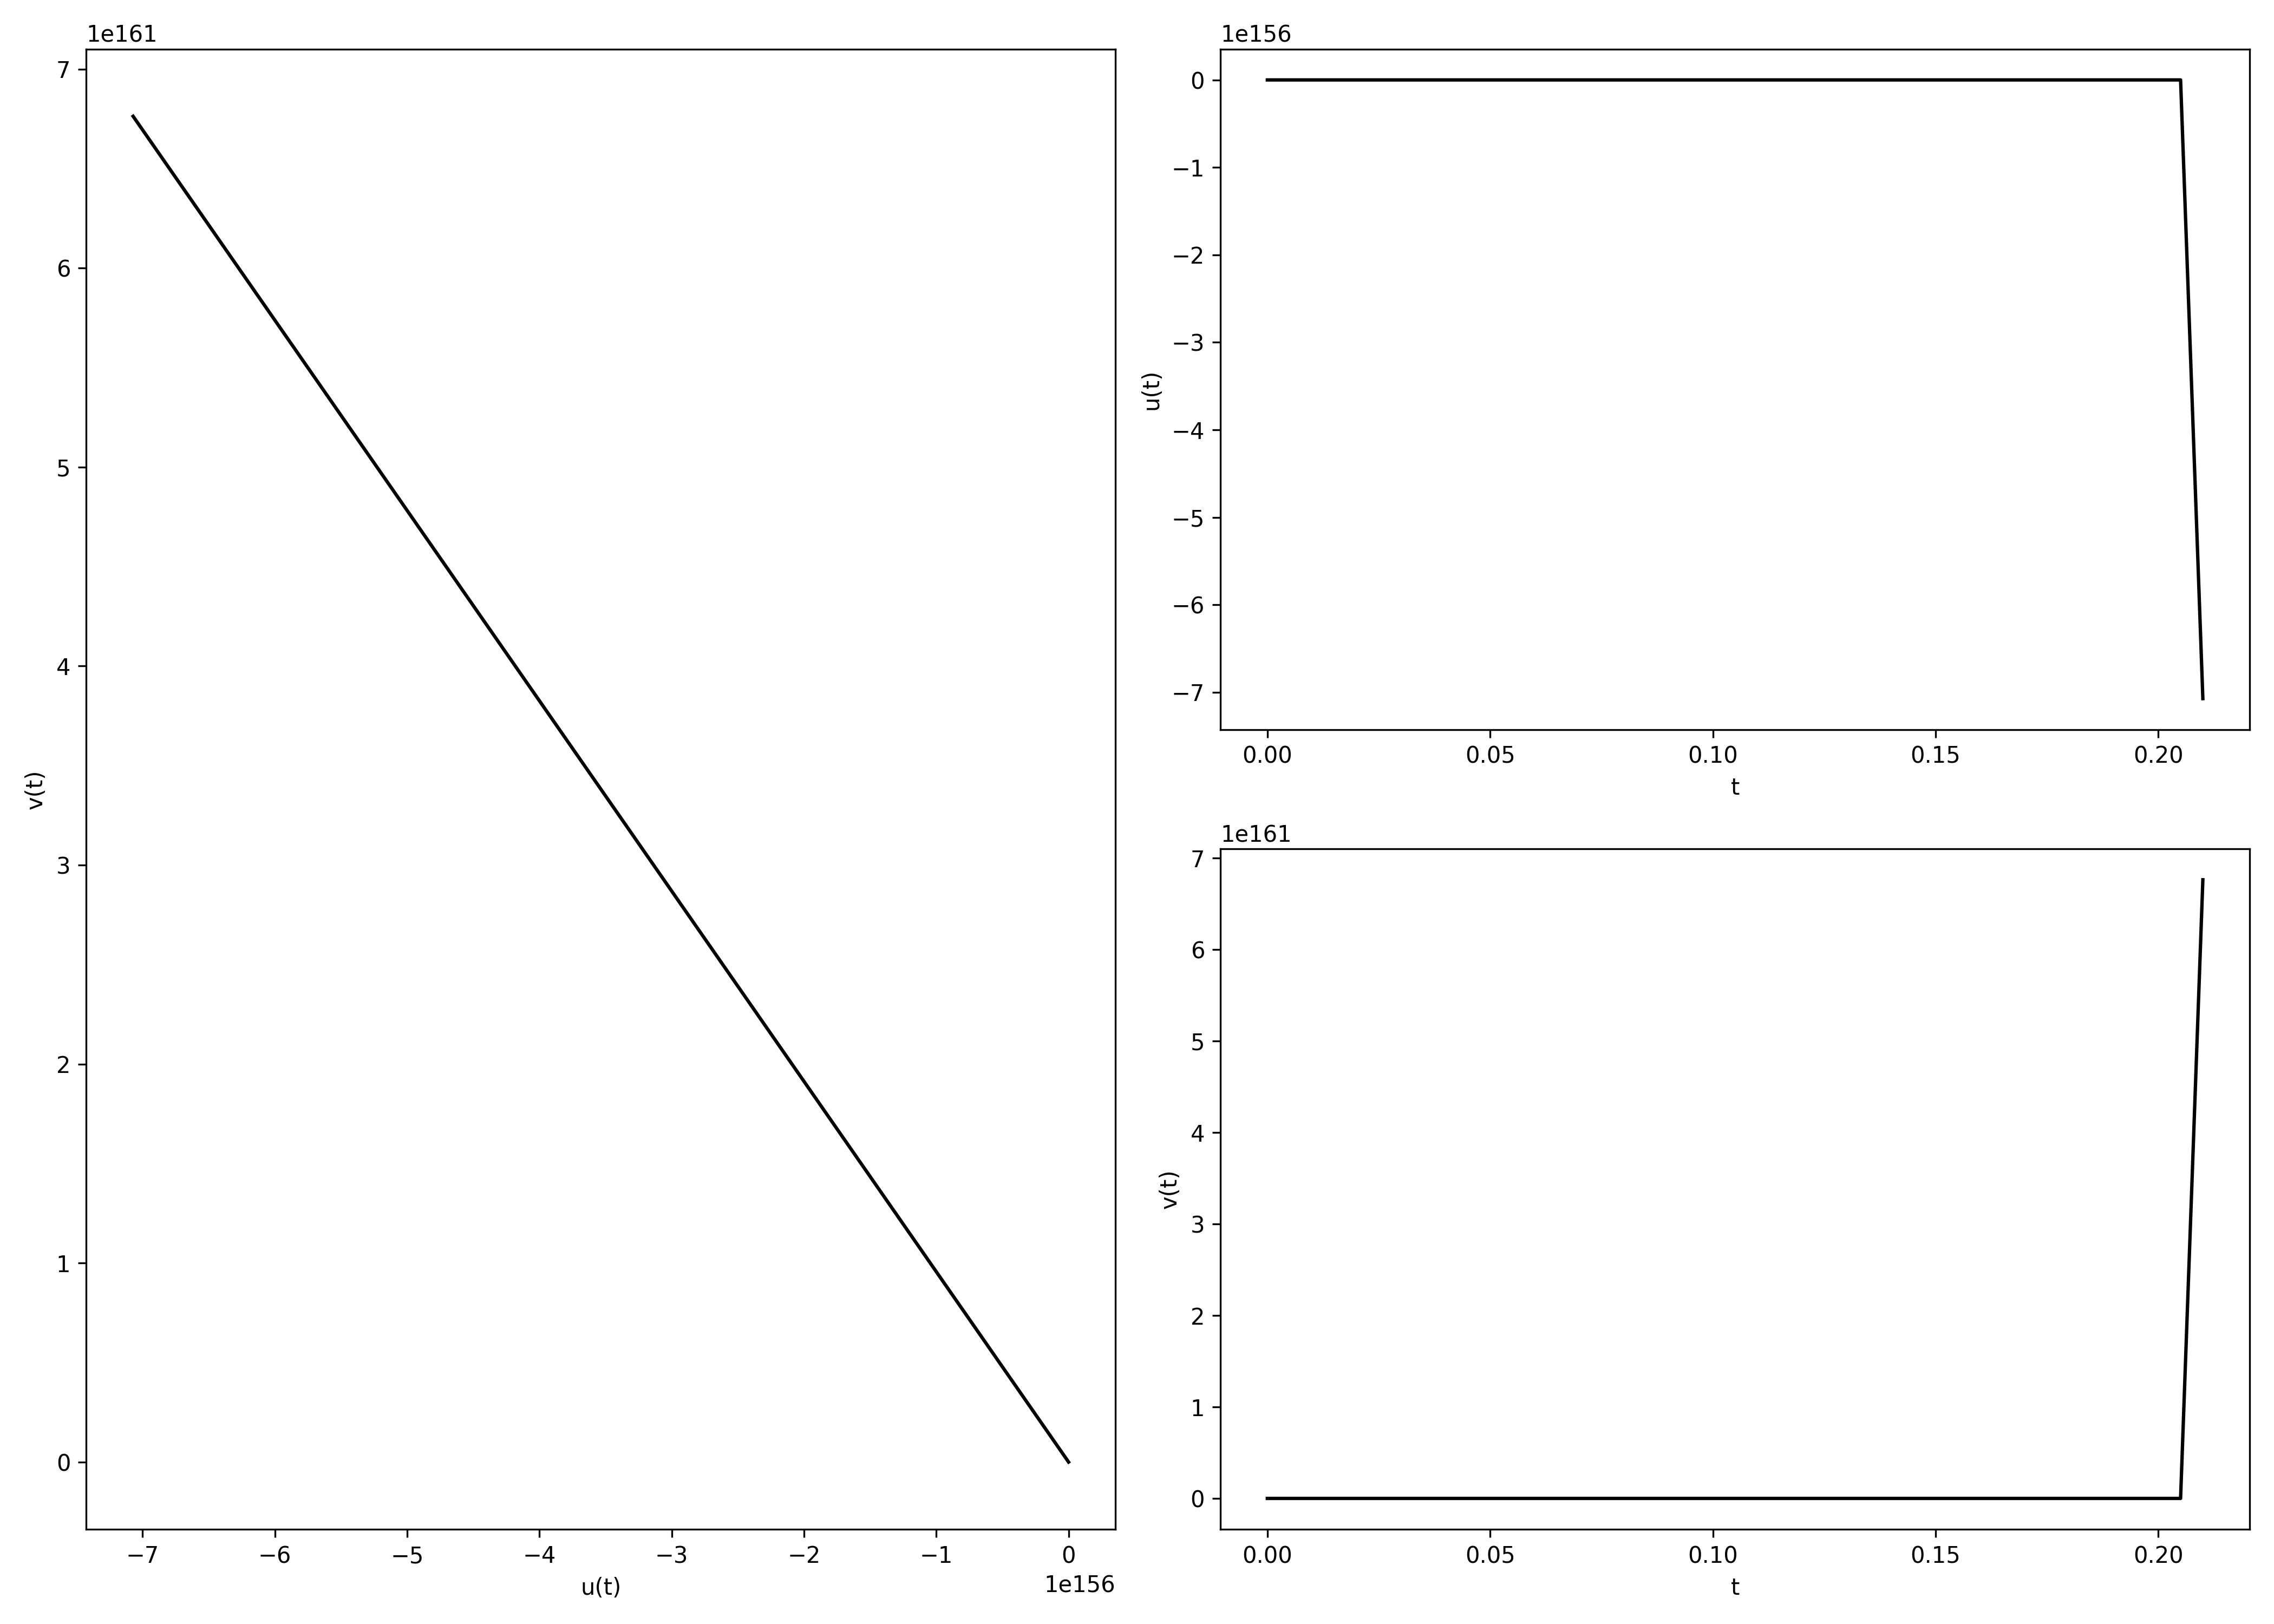
\includegraphics[scale=0.33]{u3,0v3,0a11,9b10,0c1-1,9a21,9b20,0c21,9t1,00e+01n2,00e+03.png}
\figcaption{$u_0=3.00, v_0=3.00, a_1=1.90, b_1=0.00, c_1=-1.90, a_2=1.90, b_2=0.00, c_2=1.90, T = 10, N = 2000$}
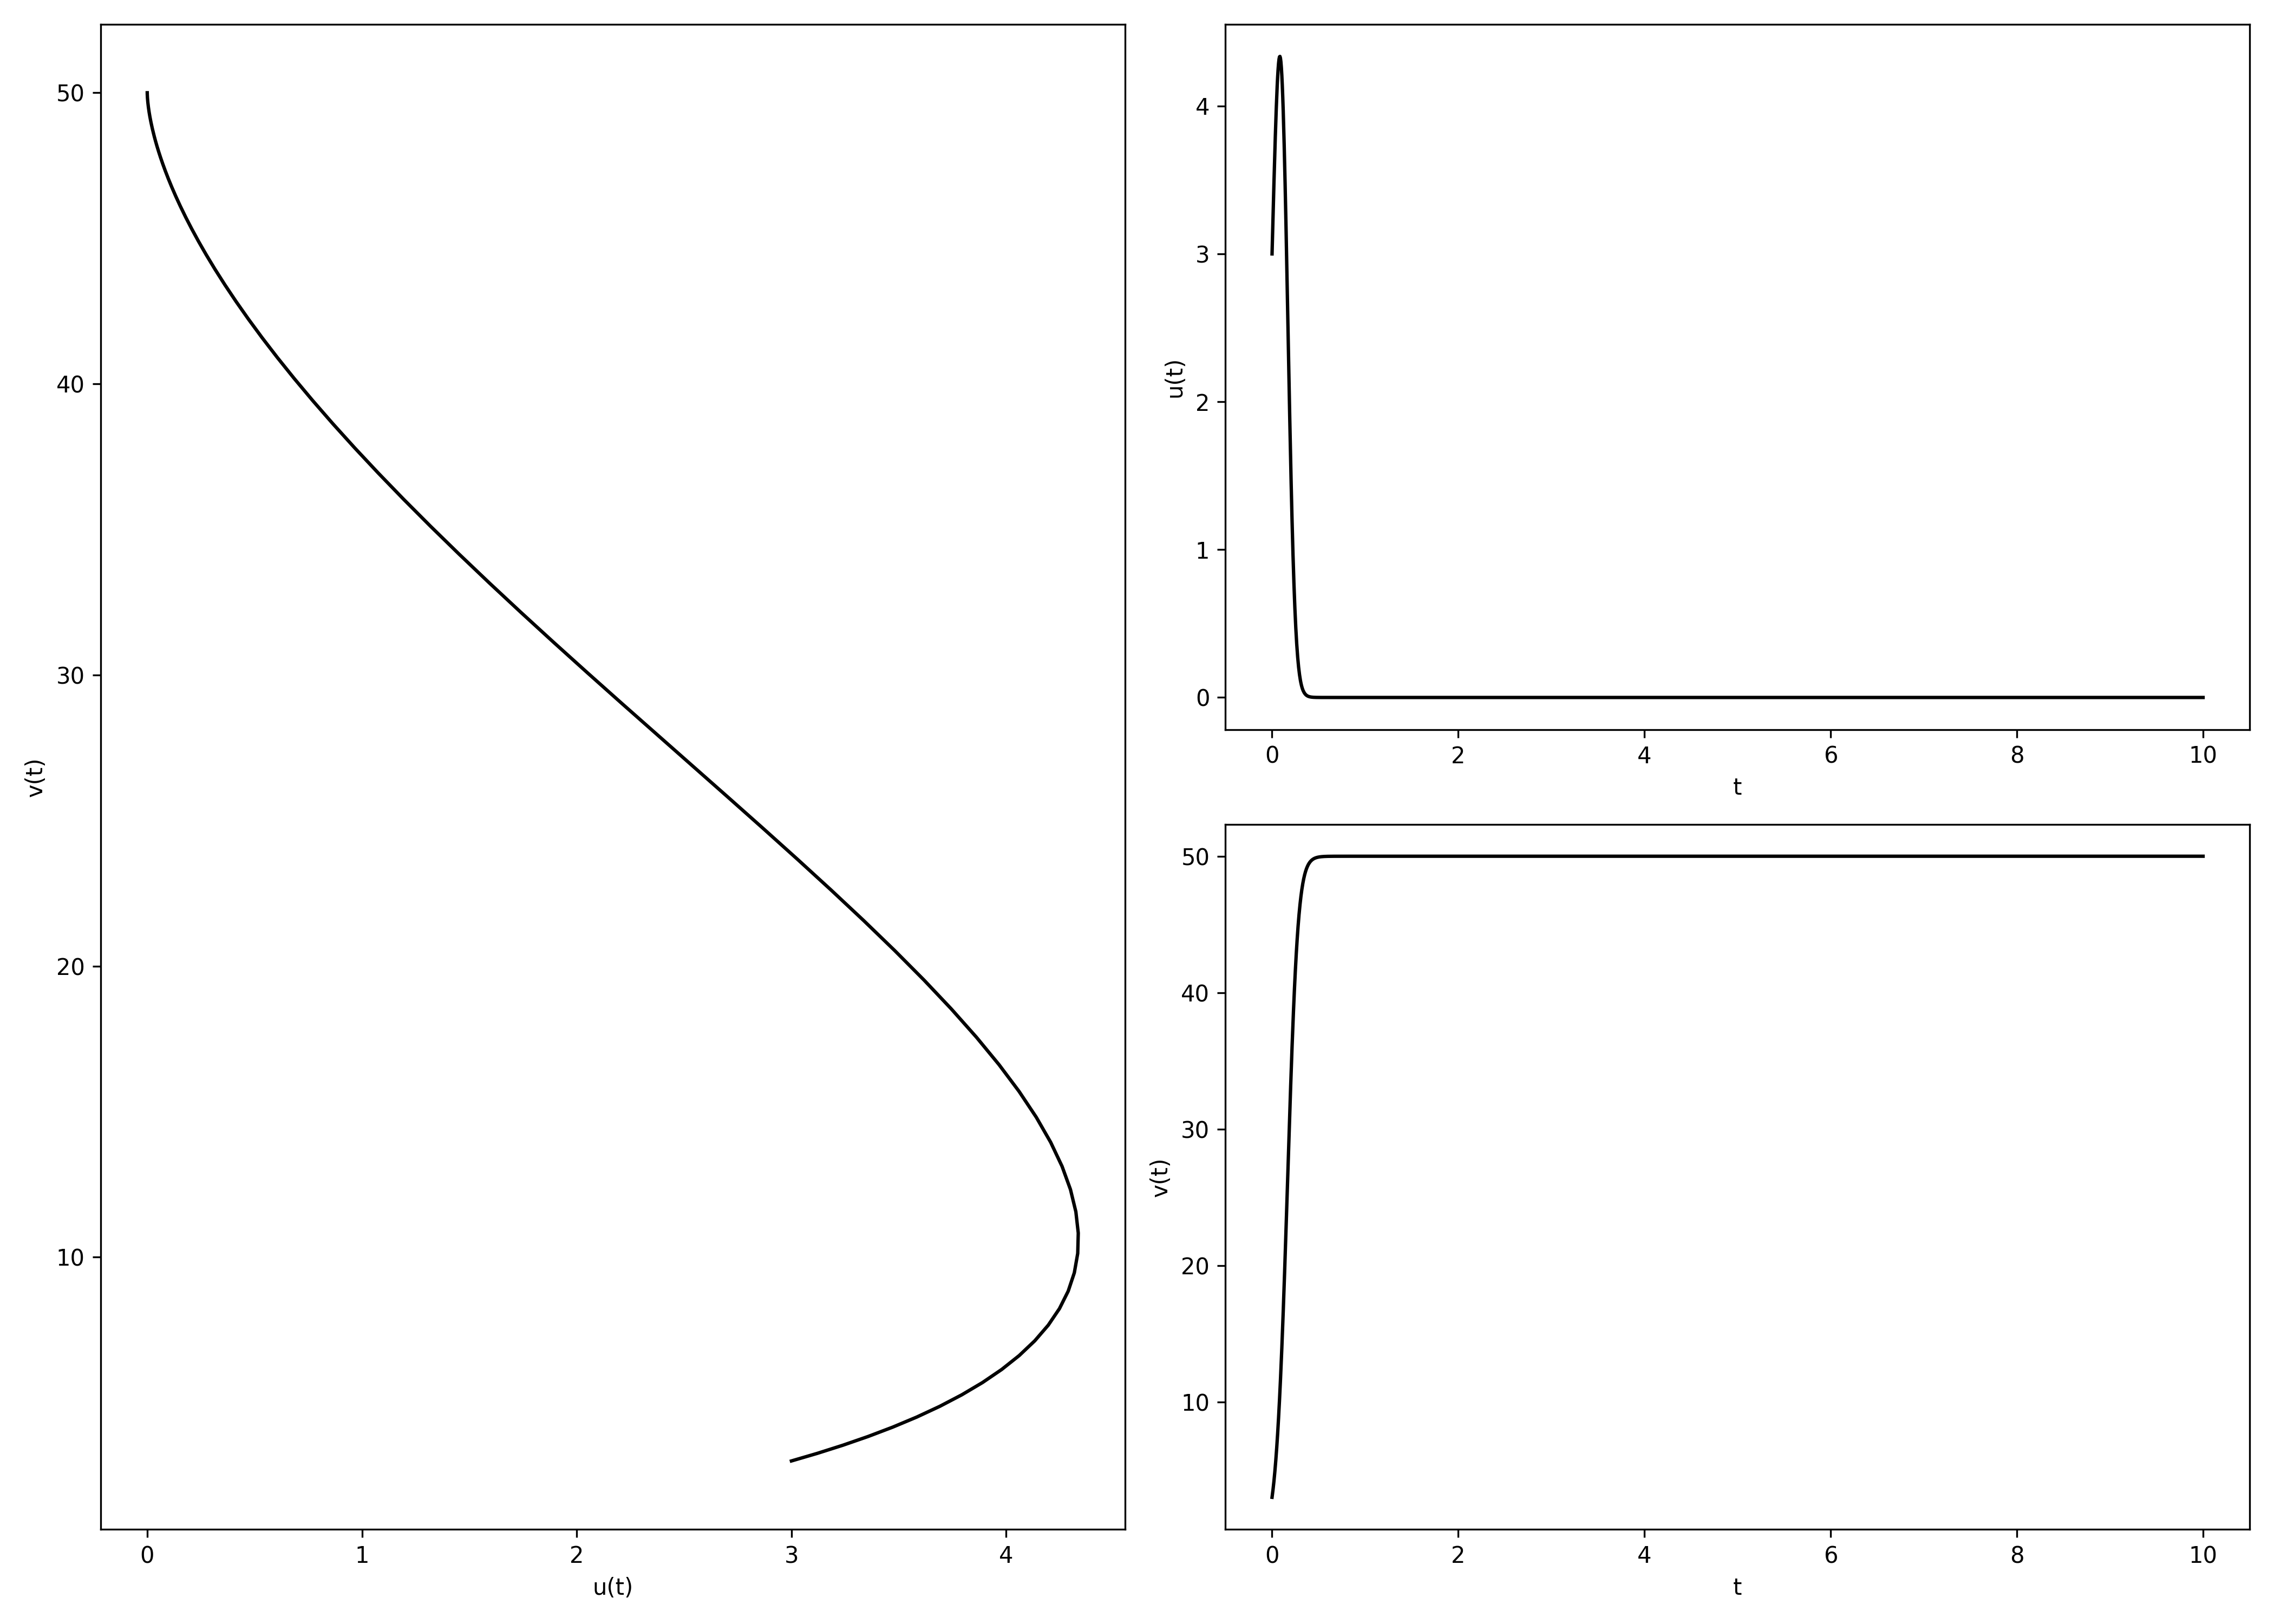
\includegraphics[scale=0.33]{u3,0v3,0a114,0b1-1,1c1-0,9a220,0b2-0,5c2-0,4t1,00e+01n2,00e+03.png}
\figcaption{$u_0=3.00, v_0=3.00, a_1=14.00, b_1=-1.10, c_1=-0.90, a_2=20.00, b_2=-0.50, c_2-=0.40, T = 10, N = 2000$}
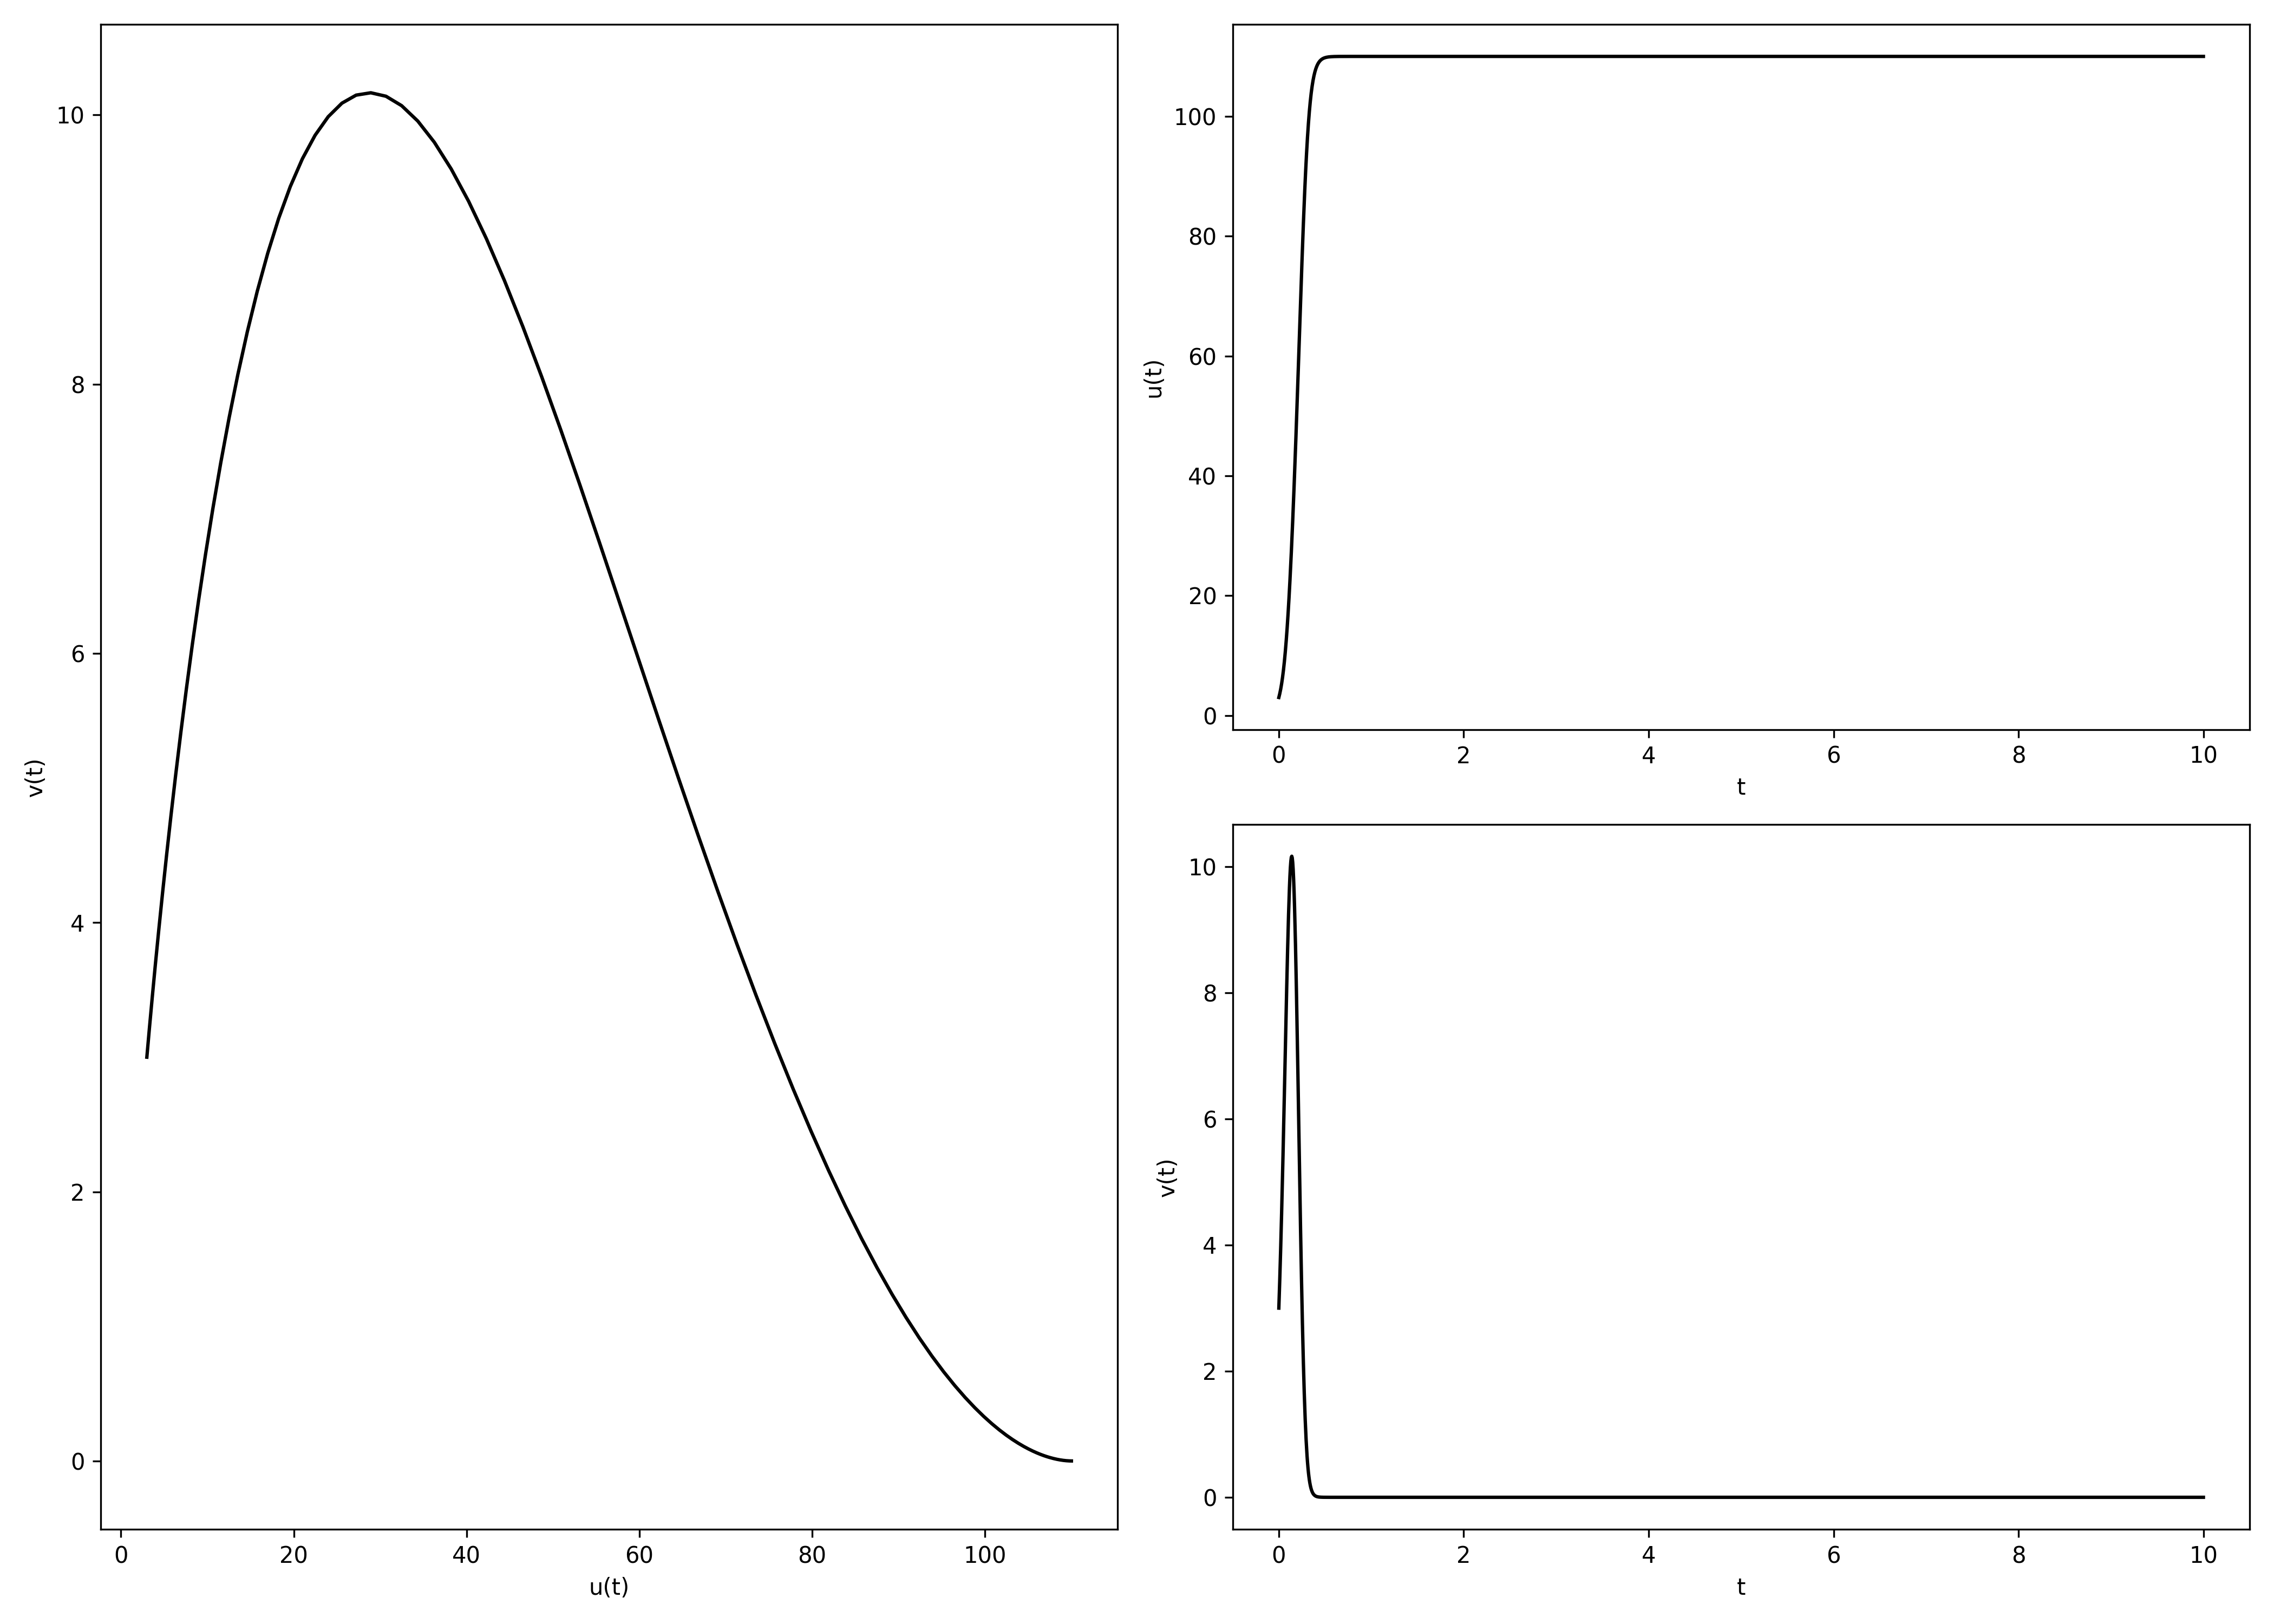
\includegraphics[scale=0.33]{u3,0v3,0a122,0b1-0,2c1-0,4a217,0b2-0,5c2-0,3t1,00e+01n2,00e+03.png}
\figcaption{$u_0=3.00, v_0=3.00, a_1=22.00, b_1=-0.20, c_1=-0.40, a_2=17.00, b_2=-0.50, c_2=-0.30, T = 10, N = 2000$}
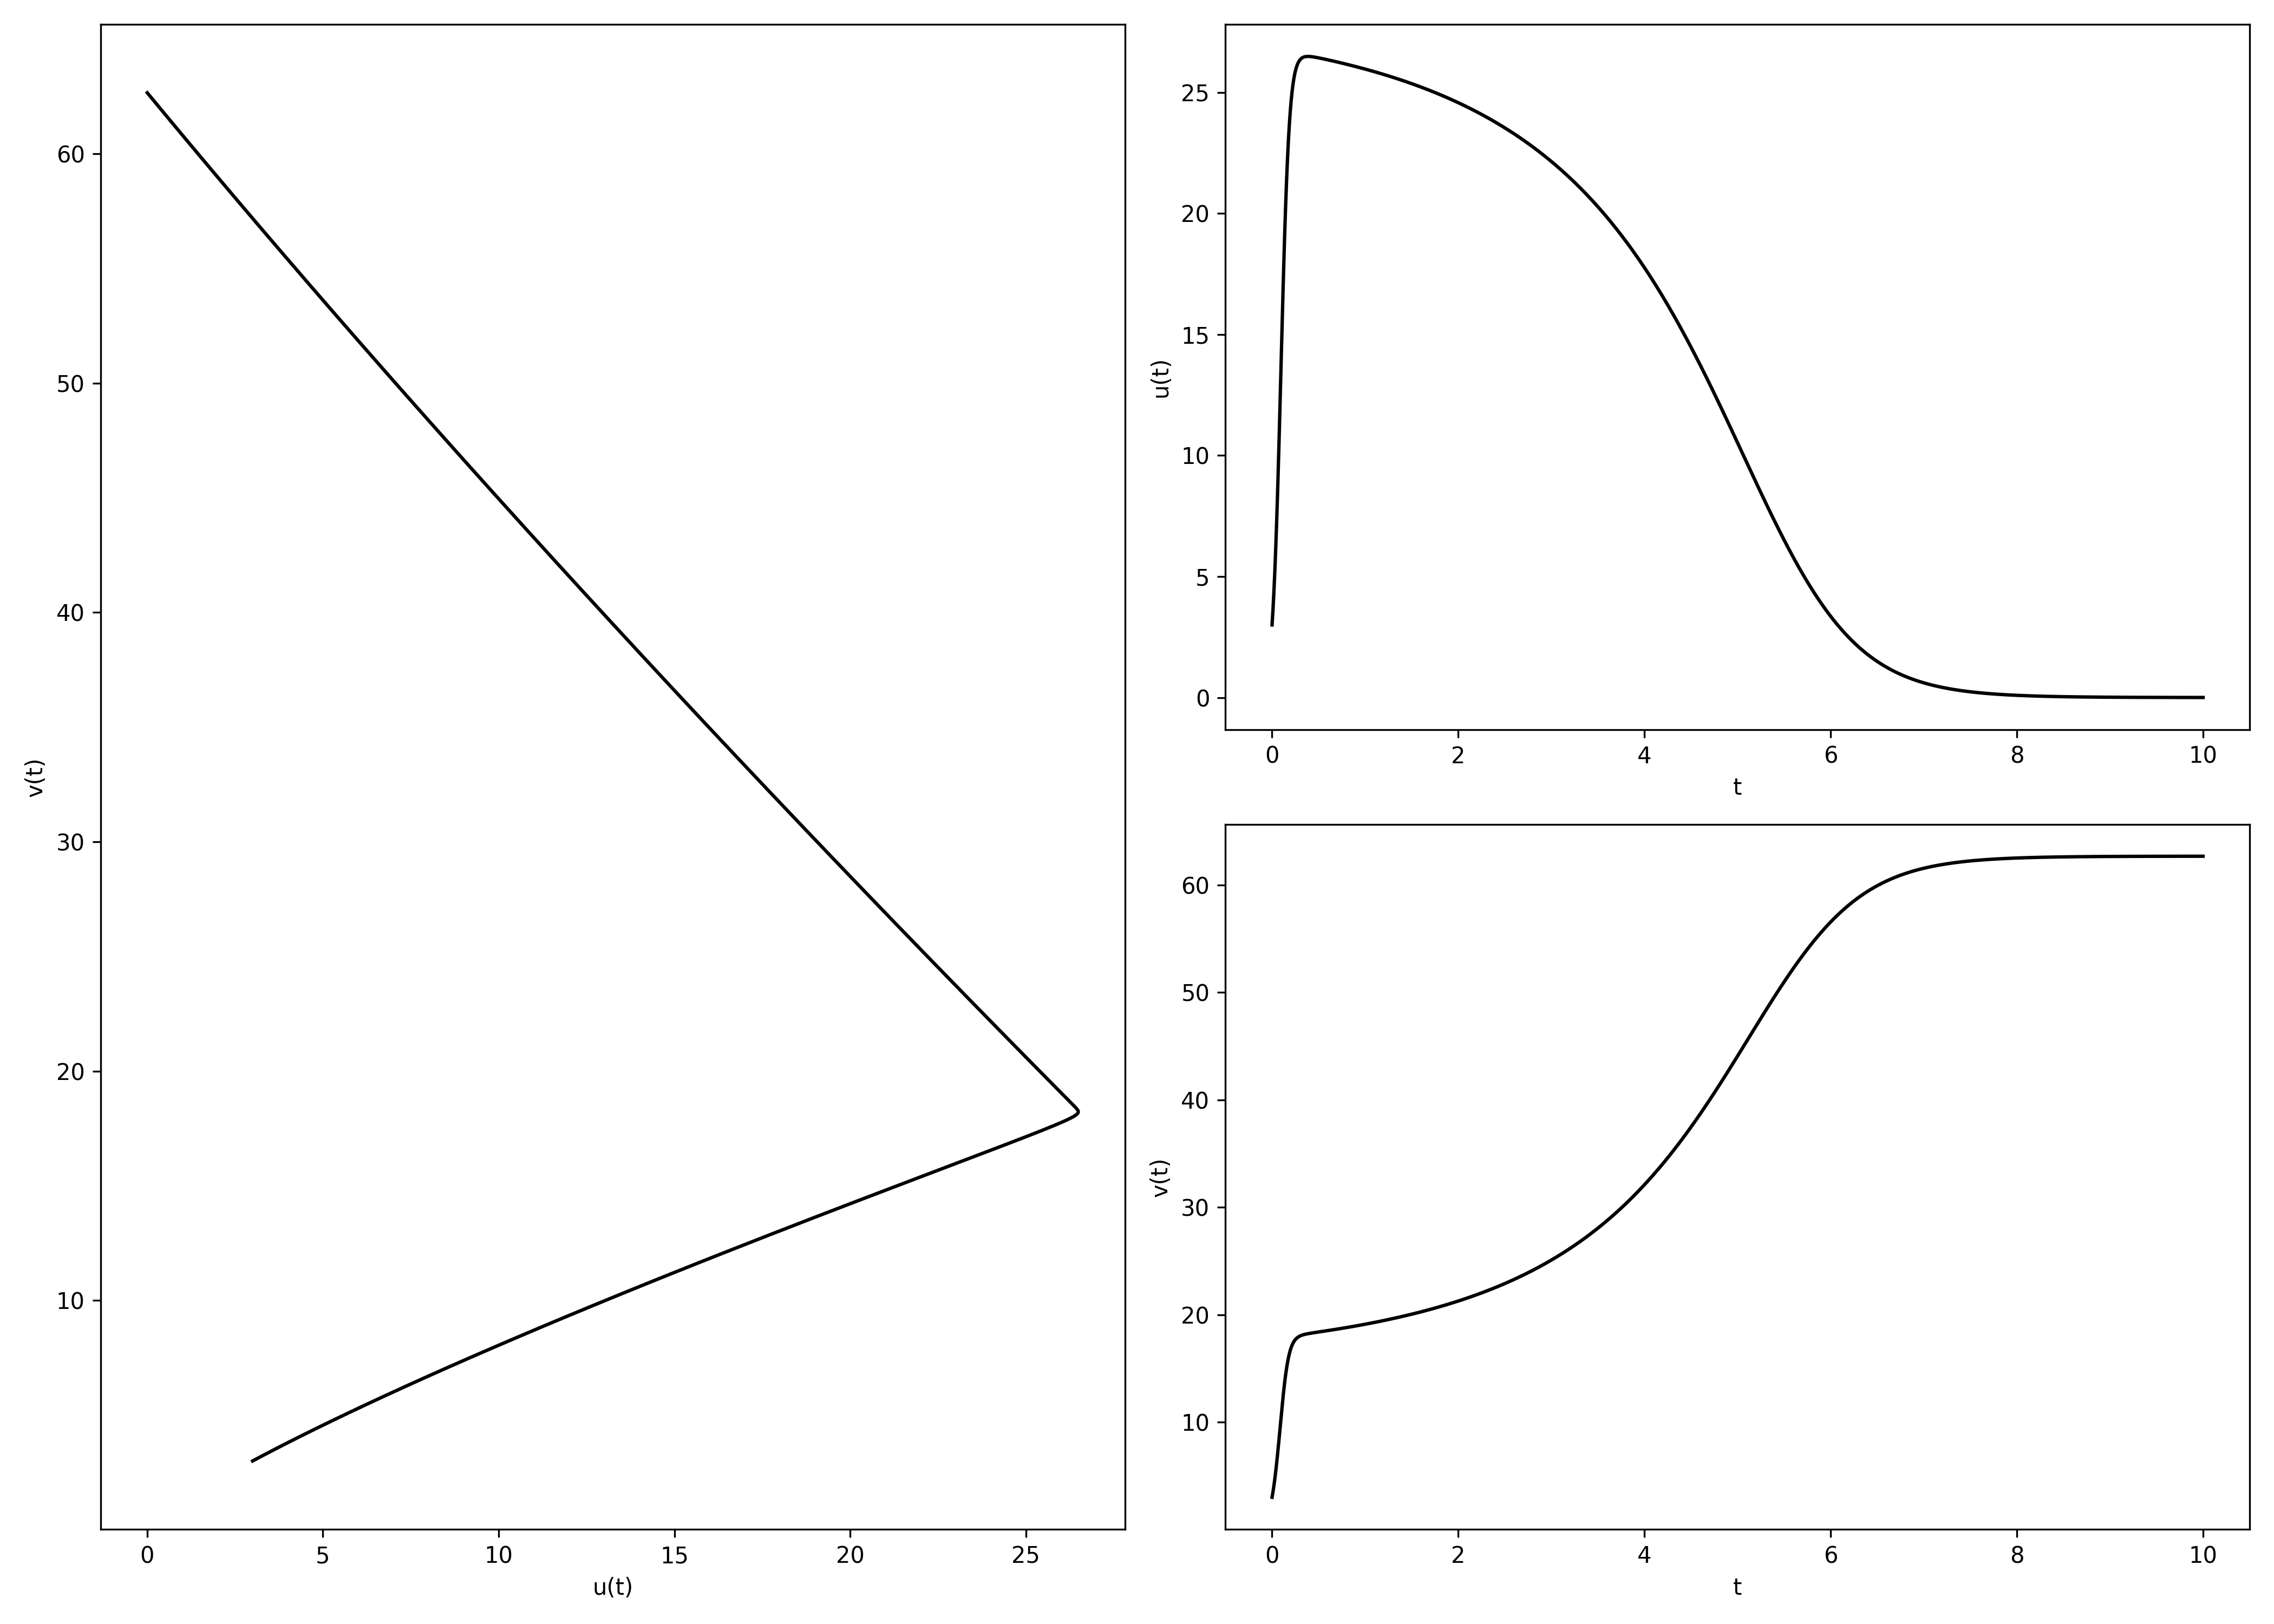
\includegraphics[scale=0.33]{u3,0v3,0a123,2b1-0,6c1-0,4a218,8b2-0,5c2-0,3t1,00e+01n2,00e+03.png}
\figcaption{$u_0=3.00, v_0=3.00, a_1=23.20, b_1=-0.60, c_1=-0.40, a_2=18.80, b_2=-0.50, c_2=-0.30, T = 10, N = 2000$}
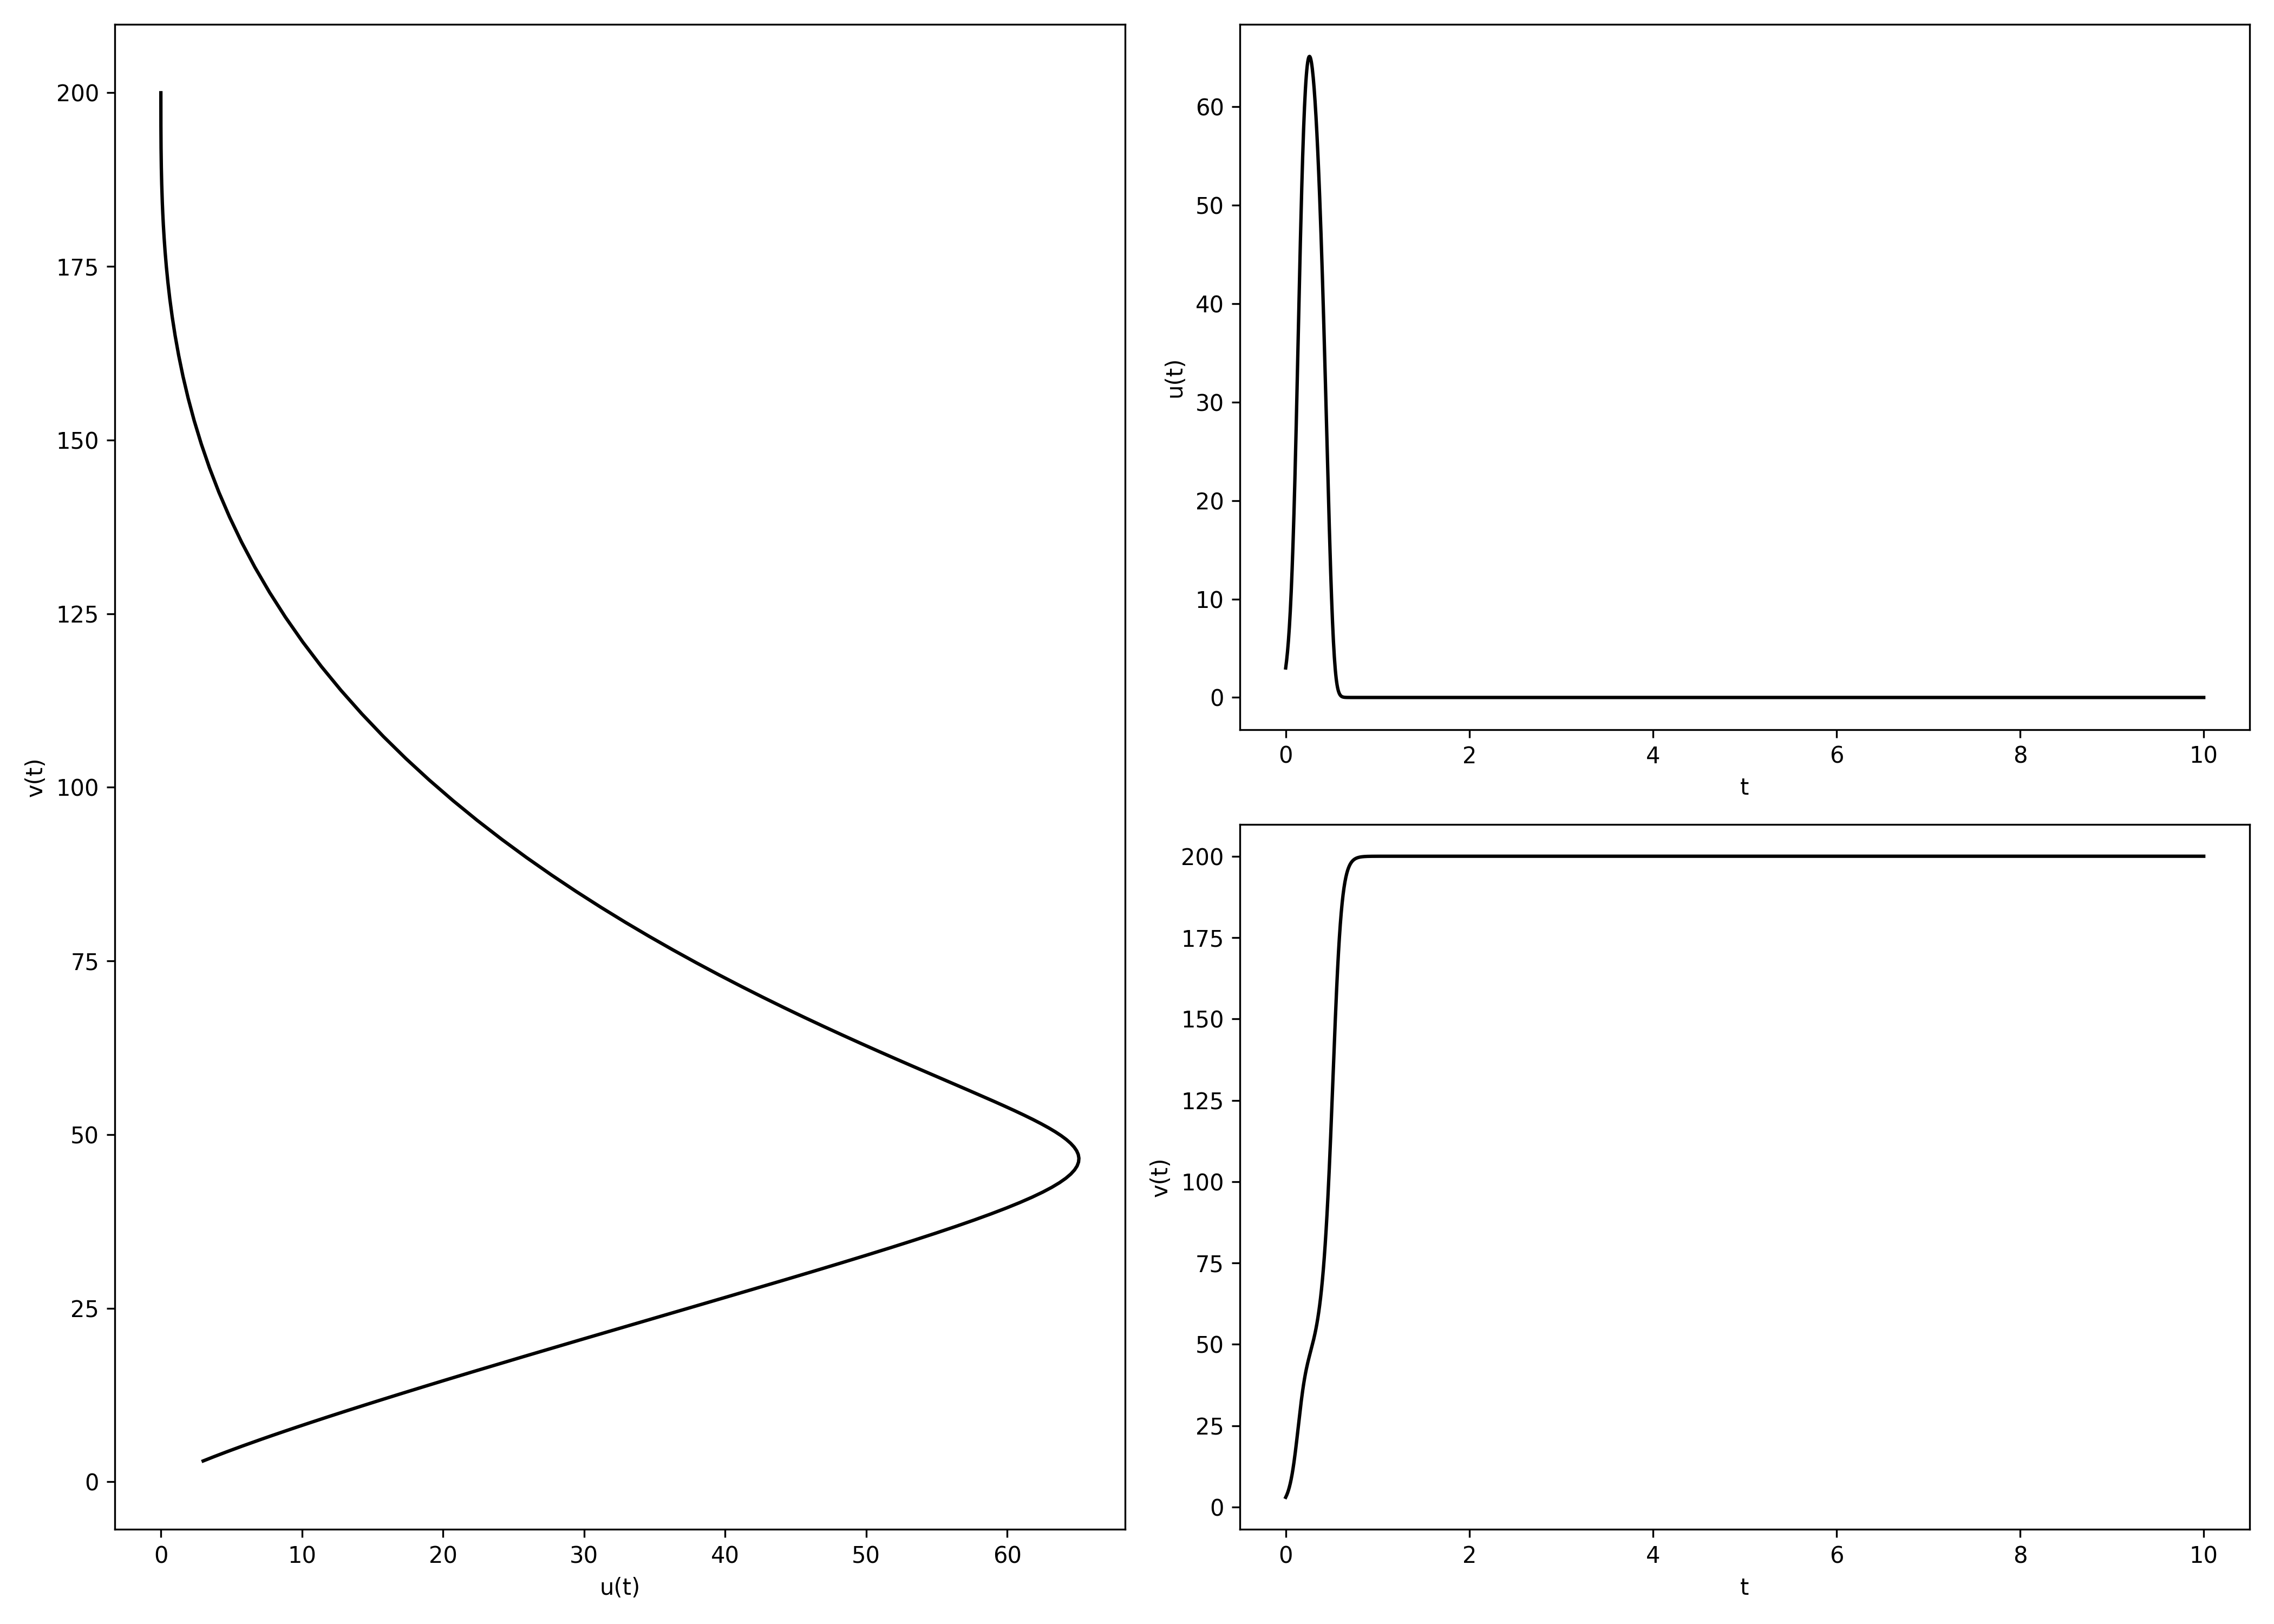
\includegraphics[scale=0.33]{u3,0v3,0a125,0b1-0,1c1-0,4a220,0b2-0,2c2-0,1t1,00e+01n2,00e+03.png}
\figcaption{$u_0=3.00, v_0=3.00, a_1=25.00, b_1=-0.10, c_1=-0.40, a_2=20.00, b_2=-0.20, c_2=-0.10, T = 10, N = 2000$}

%-----------------------考察---------------------
\section{考察}
\subsection{van der Pol 方程式}
初期値$(x_0, y_0)$によっての影響はあまりないと考えられた. しかし$(\mu, \omega)$に対して方程式が変化すると思われる.

$\mu$については, $\mu < 0$のとき, 一点に収束した. また$\mu > 0$のとき, \textbf{Limit cycle}(リミットサイクル)と呼ばれる周期軌道に収束した. $\mu = 0$については, $x, y$がそれぞれ振動し, 円を描くように発散した. よって$\mu$は概形を定めるパラメーターであった. 力学的に$\mu$は, 摩擦係数などの抵抗の係数である.

$\omega$については, $\omega = 0$のとき, 一点に収束した. また他の値において$\omega$を変更しても周期軌道の概形は変化しなかったが, 周期が$T$の値が大きくなるにつれて短くなっていったので周期に関するパラメーターである.

$T$の時間については, van der Pol 方程式は少ない時間で一点に収束か, リミットサイクルになるので$T = 100, N = 1000$で既に真の解に近い値となっていた.

$N$の分割に関しては, $N$の値を大きくするにつれてより分割が細かくなり, 精度が高くなるのだが. 同じパラメータであるにも関わらず値が異なる場合があり, 顕著に現れている例として, 図3と図21が挙げられる. なぜこのような差異が発生してしまったのかを考察すると. この場合両者は振動しながら発散していく方程式であるが, 分割がより細かいと近似解を計算する際により小さい値として計算されてしまうためであると考えられる. 今回の場合両者は$10^2$ほどオーダーが事なり数値計算の際, $\frac{1}{100}$程値が小さくなってしまうからである.

\subsection{Lotka Volterra 方程式}
初期値$(u_0, v_0)$によって解が定常解になってしまいつまらないシュミレーションになってしまう. ここで定常状態になるための必要条件は$$u_0 = \frac{a_2}{b_2}, v_0 = \frac{a_1}{c_1}$$である. 

またパラメータはそれぞれ意味を持っていて. $a_1$は$u$の出生率, $c_1$は$u, v$が出くわした時に食べられる率であり負の値を取る, $b_2$は$u, v$が出くわした際に捕食することによって子孫を増やした率, $a_2$は$v$の死亡率である.

$T$の時間についてはLotka Volterra 方程式はすぐ発散したり収束してしまうため初期値やパラメータをうまく調整して, 時間を増やさないといけないため比較実験をすることが難しかった.

$N$の分割に関しては, Lotka Volterra 方程式はすぐ発散したり一定の軌道になったりすることが多く, あまり分割を増やして細かい近似をしてもvan der Pol 方程式のように差異が現れることは少なかった.

%----------------------結論--------------------------
\section{結論}
オイラー法は収束するような解に対しては適しているが発散や振動するような解に対しては発散の速度などが変わってしまい適さない場合があるので改良する必要がある.

%---------------------参考文献----------------------
\section{参考文献}
\begin{itemize}
\item 結合van der Pol 方程式の安定性解析
\item Lotka Volterra モデルの4パラメータ固定
\item 振動する生態系 - Lotka Volterra モデル
\item 数理生態学
\end{itemize}

%---------------------感想-------------------------
\section{感想}
パラメーターや初期値を見つけるのが大変でLotka Volterra 方程式に関しては調べていく際に出てくる, 円のような動きをする気配がなくそれぞれのパラメータを乱数で回し何回も試行していく中で, 円のような動きに近いものを見つけてはそのパラメータの付近で新たに乱数を回して今回の実験のようなグラフに行くつくことができとても大変であった.

また, 一個前の数値解のみを参照して計算を続けてしまっているからオイラー法は差異が出てしまうのだと思われる. ここでRunge-Kutta 法のように全ての数値解を使うような計算をするとより真の解との差異が減っていきより良い近似解へとなるのではないかと思い, Runge-Kutta 法でも同じような近似解を出したいと思った.
\end{document}
